%%% Hlavní soubor. Zde se definují základní parametry a odkazuje se na ostatní části. %%%

%% Verze pro jednostranný tisk:
% Okraje: levý 40mm, pravý 25mm, horní a dolní 25mm
% (ale pozor, LaTeX si sám přidává 1in)
\documentclass[12pt,a4paper]{report}
\setlength\textwidth{145mm}
\setlength\textheight{247mm}
\setlength\oddsidemargin{15mm}
\setlength\evensidemargin{15mm}
\setlength\topmargin{0mm}
\setlength\headsep{0mm}
\setlength\headheight{0mm}
% \openright zařídí, aby následující text začínal na pravé straně knihy
\let\openright=\clearpage

%% Pokud tiskneme oboustranně:
% \documentclass[12pt,a4paper,twoside,openright]{report}
% \setlength\textwidth{145mm}
% \setlength\textheight{247mm}
% \setlength\oddsidemargin{14.2mm}
% \setlength\evensidemargin{0mm}
% \setlength\topmargin{0mm}
% \setlength\headsep{0mm}
% \setlength\headheight{0mm}
% \let\openright=\cleardoublepage

%% Vytváříme PDF/A-2u
\usepackage[a-2u]{pdfx}

%% Přepneme na českou sazbu a fonty Latin Modern
\usepackage[czech]{babel}
\usepackage{lmodern}
\usepackage[T1]{fontenc}
\usepackage{textcomp}

%% Použité kódování znaků: obvykle latin2, cp1250 nebo utf8:
\usepackage[utf8]{inputenc}

%%% Další užitečné balíčky (jsou součástí běžných distribucí LaTeXu)
\usepackage{amsmath}        % rozšíření pro sazbu matematiky
\usepackage{amsfonts}       % matematické fonty
\usepackage{amsthm}         % sazba vět, definic apod.
\usepackage{bbding}         % balíček s nejrůznějšími symboly
			    % (čtverečky, hvězdičky, tužtičky, nůžtičky, ...)
\usepackage{bm}             % tučné symboly (příkaz \bm)
\usepackage{graphicx}       % vkládání obrázků
\usepackage{fancyvrb}       % vylepšené prostředí pro strojové písmo
\usepackage{indentfirst}    % zavede odsazení 1. odstavce kapitoly
\usepackage{natbib}         % zajištuje možnost odkazovat na literaturu
			    % stylem AUTOR (ROK), resp. AUTOR [ČÍSLO]
\usepackage[nottoc]{tocbibind} % zajistí přidání seznamu literatury,
                            % obrázků a tabulek do obsahu
\usepackage{icomma}         % inteligetní čárka v matematickém módu
\usepackage{dcolumn}        % lepší zarovnání sloupců v tabulkách
\usepackage{booktabs}       % lepší vodorovné linky v tabulkách
\usepackage{paralist}       % lepší enumerate a itemize
\usepackage{xcolor}         % barevná sazba
\usepackage{dirtree}
\usepackage{listings}

%%% Údaje o práci

% Název práce v jazyce práce (přesně podle zadání)
\def\NazevPrace{Vylepšení agregace dotazovacího enginu pro grafové databáze}

% Název práce v angličtině
\def\NazevPraceEN{Improvement of data aggregation in query engine for graph databases}

% Jméno autora
\def\AutorPrace{Martin Gora}

% Rok odevzdání
\def\RokOdevzdani{2021}

% Název katedry nebo ústavu, kde byla práce oficiálně zadána
% (dle Organizační struktury MFF UK, případně plný název pracoviště mimo MFF)
\def\Katedra{Katedra softwarového inženýrství}
\def\KatedraEN{Department of Software Engineering}

% Jedná se o katedru (department) nebo o ústav (institute)?
\def\TypPracoviste{Katedra}
\def\TypPracovisteEN{Department}

% Vedoucí práce: Jméno a příjmení s~tituly
\def\Vedouci{Mgr. Tomáš Faltín}

% Pracoviště vedoucího (opět dle Organizační struktury MFF)
\def\KatedraVedouciho{Katedra softwarového inženýrství}
\def\KatedraVedoucihoEN{Department of Software Engineering}

% Studijní program a obor
\def\StudijniProgram{Informatika}
\def\StudijniObor{Softwarové a datové inženýrství}

% Nepovinné poděkování (vedoucímu práce, konzultantovi, tomu, kdo
% zapůjčil software, literaturu apod.)
\def\Podekovani{%
Chtěl bych poděkovat mému vedoucímu Mgr. Tomáši Faltínovi za jeho pomoc, ochotu a nadšení při zpracovávání daného tématu.
Dále bych chtěl poděkovat rodině, která mi poskytla zázemí pro práci a plnou podporu.
}

% Abstrakt (doporučený rozsah cca 80-200 slov; nejedná se o zadání práce)
\def\Abstrakt{%
Proudové systémy mají vůči dotazovacím enginům pro grafové databáze výhodu při agregaci dat (části Group by a Order by), protože jim stačí uchovávat pouze agregované prvky, ale zase nedokáží provádět vyhledávání vzoru.

V této práci jsme vytvořili statickou grafovou databázi s Labeled-property datovým modelem a pro ni dotazovací engine, který agreguje data klasickým přístupem až po dokončení vyhledávání vzoru.
Dotazovací engine jsme následně upravili po vzoru proudových systémů tak, aby prováděl agregace již v průběhu vyhledávání vzoru.
Cílem této práce bylo zjistit, zda danou úpravou dokážeme urychlit zpracování dotazů.

Pro upravený i klasický přístup jsme navrhli a implementovali několik jednovláknových i paralelních řešení.
Řešení jsme porovnali v rychlosti zpracování dotazů na reálných grafech s uměle vygenerovanými hodnotami vlastností.
Zjistili jsme, že existují situace, kdy zmíněnou úpravou došlo k urychlení zpracování dotazů.
Konkrétně se tak stalo pro paralelní řešení části Order by při třídění pomocí hodnot vlastností, jednovláknové řešení části Group by a posledně pro jednovláknové i paralelní řešení Single group Group by (dotaz obsahuje agregační funkce a nemá část Group by).
}
\def\AbstraktEN{%
Abstract.
}

% 3 až 5 klíčových slov (doporučeno), každé uzavřeno ve složených závorkách
\def\KlicovaSlova{%
{grafové databáze} {agregace dat} {proudové systémy}
}
\def\KlicovaSlovaEN{%
{graph databases} {data aggregation} {streaming systems}
}

%% Balíček hyperref, kterým jdou vyrábět klikací odkazy v PDF,
%% ale hlavně ho používáme k uložení metadat do PDF (včetně obsahu).
%% Většinu nastavítek přednastaví balíček pdfx.
\hypersetup{unicode}
\hypersetup{breaklinks=true}

%% Definice různých užitečných maker (viz popis uvnitř souboru)
%%% Tento soubor obsahuje definice různých užitečných maker a prostředí %%%
%%% Další makra připisujte sem, ať nepřekáží v ostatních souborech.     %%%

%%% Drobné úpravy stylu

% Tato makra přesvědčují mírně ošklivým trikem LaTeX, aby hlavičky kapitol
% sázel příčetněji a nevynechával nad nimi spoustu místa. Směle ignorujte.
\makeatletter
\def\@makechapterhead#1{
  {\parindent \z@ \raggedright \normalfont
   \Huge\bfseries \thechapter. #1
   \par\nobreak
   \vskip 20\p@
}}
\def\@makeschapterhead#1{
  {\parindent \z@ \raggedright \normalfont
   \Huge\bfseries #1
   \par\nobreak
   \vskip 20\p@
}}
\makeatother

% Toto makro definuje kapitolu, která není očíslovaná, ale je uvedena v obsahu.
\def\chapwithtoc#1{
\chapter*{#1}
\addcontentsline{toc}{chapter}{#1}
}

% Trochu volnější nastavení dělení slov, než je default.
\lefthyphenmin=2
\righthyphenmin=2

% Zapne černé "slimáky" na koncích řádků, které přetekly, abychom si
% jich lépe všimli.
\overfullrule=1mm

%%% Makra pro definice, věty, tvrzení, příklady, ... (vyžaduje baliček amsthm)

\theoremstyle{plain}
\newtheorem{veta}{Věta}
\newtheorem{lemma}[veta]{Lemma}
\newtheorem{tvrz}[veta]{Tvrzení}

\theoremstyle{plain}
\newtheorem{definice}{Definice}

\theoremstyle{remark}
\newtheorem*{dusl}{Důsledek}
\newtheorem*{pozn}{Poznámka}
\newtheorem*{prikl}{Příklad}

%%% Prostředí pro důkazy

\newenvironment{dukaz}{
  \par\medskip\noindent
  \textit{Důkaz}.
}{
\newline
\rightline{$\qedsymbol$}
}

%%% Prostředí pro sazbu kódu, případně vstupu/výstupu počítačových
%%% programů. (Vyžaduje balíček fancyvrb -- fancy verbatim.)

\DefineVerbatimEnvironment{code}{Verbatim}{fontsize=\small, frame=single}

%%% Prostor reálných, resp. přirozených čísel
\newcommand{\R}{\mathbb{R}}
\newcommand{\N}{\mathbb{N}}

%%% Užitečné operátory pro statistiku a pravděpodobnost
\DeclareMathOperator{\pr}{\textsf{P}}
\DeclareMathOperator{\E}{\textsf{E}\,}
\DeclareMathOperator{\var}{\textrm{var}}
\DeclareMathOperator{\sd}{\textrm{sd}}

%%% Příkaz pro transpozici vektoru/matice
\newcommand{\T}[1]{#1^\top}

%%% Vychytávky pro matematiku
\newcommand{\goto}{\rightarrow}
\newcommand{\gotop}{\stackrel{P}{\longrightarrow}}
\newcommand{\maon}[1]{o(n^{#1})}
\newcommand{\abs}[1]{\left|{#1}\right|}
\newcommand{\dint}{\int_0^\tau\!\!\int_0^\tau}
\newcommand{\isqr}[1]{\frac{1}{\sqrt{#1}}}

%%% Vychytávky pro tabulky
\newcommand{\pulrad}[1]{\raisebox{1.5ex}[0pt]{#1}}
\newcommand{\mc}[1]{\multicolumn{1}{c}{#1}}


%% Titulní strana a různé povinné informační strany
\begin{document}
%%% Titulní strana práce a další povinné informační strany

%%% Titulní strana práce

\pagestyle{empty}
\hypersetup{pageanchor=false}

\begin{center}

\centerline{\mbox{
\includegraphics[width=166mm]{../img/logo-cs.pdf}}}

\vspace{-8mm}
\vfill

{\bf\Large BAKALÁŘSKÁ PRÁCE}

\vfill

{\LARGE\AutorPrace}

\vspace{15mm}

{\LARGE\bfseries\NazevPrace}

\vfill

\Katedra

\vfill

{
\centerline{\vbox{\halign{\hbox to 0.45\hsize{\hfil #}&\hskip 0.5em\parbox[t]{0.45\hsize}{\raggedright #}\cr
Vedoucí bakalářské práce:&\Vedouci \cr
\noalign{\vspace{2mm}}
Studijní program:&\StudijniProgram \cr
\noalign{\vspace{2mm}}
Studijní obor:&\StudijniObor \cr
}}}}

\vfill

% Zde doplňte rok
Praha \RokOdevzdani

\end{center}

\newpage

%%% Následuje vevázaný list -- kopie podepsaného "Zadání bakalářské práce".
%%% Toto zadání NENÍ součástí elektronické verze práce, nescanovat.

%%% Strana s čestným prohlášením k bakalářské práci

\openright
\hypersetup{pageanchor=true}
\pagestyle{plain}
\pagenumbering{roman}
\vglue 0pt plus 1fill

\noindent
Prohlašuji, že jsem tuto bakalářskou práci vypracoval(a) samostatně a výhradně
s~použitím citovaných pramenů, literatury a dalších odborných zdrojů.
Tato práce nebyla využita k získání jiného nebo stejného titulu.

\medskip\noindent
Beru na~vědomí, že se na moji práci vztahují práva a povinnosti vyplývající
ze zákona č. 121/2000 Sb., autorského zákona v~platném znění, zejména skutečnost,
že Univerzita Karlova má právo na~uzavření licenční smlouvy o~užití této
práce jako školního díla podle §60 odst. 1 autorského zákona.

\vspace{10mm}

\hbox{\hbox to 0.5\hsize{%
V \hbox to 6em{\dotfill} dne \hbox to 6em{\dotfill}
\hss}\hbox to 0.5\hsize{\dotfill\quad}}
\smallskip
\hbox{\hbox to 0.5\hsize{}\hbox to 0.5\hsize{\hfil Podpis autora\hfil}}

\vspace{20mm}
\newpage

%%% Poděkování

\openright

\noindent
\Podekovani

\newpage

%%% Povinná informační strana bakalářské práce

\openright

\vbox to 0.5\vsize{
\setlength\parindent{0mm}
\setlength\parskip{5mm}

Název práce:
\NazevPrace

Autor:
\AutorPrace

\TypPracoviste:
\Katedra

Vedoucí bakalářské práce:
\Vedouci, \KatedraVedouciho

Abstrakt:
\Abstrakt

Klíčová slova:
\KlicovaSlova

\vss}
\clearpage
\nobreak\vbox to 0.49\vsize{
\setlength\parindent{0mm}
\setlength\parskip{5mm}

Title:
\NazevPraceEN

Author:
\AutorPrace

\TypPracovisteEN:
\KatedraEN

Supervisor:
\Vedouci, \KatedraVedoucihoEN

Abstract:
\AbstraktEN

Keywords:
\KlicovaSlovaEN

\vss}

\newpage

\openright
\pagestyle{plain}
\pagenumbering{arabic}
\setcounter{page}{1}


%%% Strana s automaticky generovaným obsahem bakalářské práce

\tableofcontents

%%% Jednotlivé kapitoly práce jsou pro přehlednost uloženy v samostatných souborech
\chapter*{Úvod}
\addcontentsline{toc}{chapter}{Úvod}

\section*{Grafové databáze}

Grafové databáze zažívají v dnešní době rozkvět, například kvůli nutnosti analyzovat data na sociálních sítích.
Pro grafové databáze existují dva hlavní modely dat: RDF \citep{rdf} a Labeled-property (sekce \ref{req.propGraph}).
RDF je převážně používán k popisu informací na internetu. 
Labeled-property model se používá k obecnému popisu grafových dat.
Grafové databáze poskytují dvě základní možnosti analýzy dat:
\begin{itemize}
\item
První možnost je \textbf{spouštění algoritmů} nad uloženými grafovými daty.
Samotná skupina používaných algoritmů obsahuje od jednoduchých algoritmů jako hledání nejkratší cesty až po komplexní algoritmy jako Community detection \citep[str. 115]{graphAlg}.
Program, který poskytuje tuto možnost analýzy dat, budeme označovat jako \textbf{analytický engine}.
\item
Druhá možnost je \textbf{vykonávání dotazů} pomocí dotazovacího jazyka.
Dotazy jsou zde podobné SQL dotazům.
Pro RDF model to je například jazyk SPARQL \citep{sparql}.
Pro Labeled-property to je PGQL \citep{pgql} nebo openCypher \citep{openCypher}.
Dotazy obsahují základní části se stejnou logikou z SQL jako \textit{Select}, \textit{Order by}, \textit{Group by}, \textit{Having} a podobně.
Hlavní rozdíl těchto dotazovacích jazyků od SQL je ten, že specifikují výběr dat pomocí sekvence vrcholů a hran.
Pro PGQL a openCypher to je část dotazu \textit{Match} a pro SPARQL to je část dotazu \textit{Where}.
Tyto sekvence tvoří podgraf (vzor), který bude vyhledáván v grafu.
V moment nalezení všech podgrafů jsou na výsledcích aplikovány další části jako \textit{Group by}, \textit{Order by}, a podobně.
Tomuto se říká vyhledávání vzoru, nebo-li pattern matching.
Program, který poskytuje tuto možnost analýzy dat, budeme označovat jako \textbf{dotazovací engine}.
\end{itemize}

\section*{Proudové systémy}

Na druhé straně množství dat ke zpracování poslední dobou značně roste a nastává problém při jejich zpracování, protože se všechny nevejdou do paměti nebo dochází k jejich velmi častým změnám.  
Z tohoto důvodu začaly vznikat takzvané \textbf{proudové systémy} \citep{streaming}.
Proudové systémy obecně pracují s daty, která jsou potencionálně nekonečná a nevlezou se do paměti.
V takovém případě jsou data reprezentovány formou tekoucího „\textbf{proudu}“ (stream).
Obecně uvnitř proudu mohou být jakákoliv data, například prováděné akce, události změn nebo transakce.
Programy pracující s proudem dat sledují jen jeho určitý bod a zpracovávají data v moment kdy protékají daným bodem.
Výsledně program vidí jen útržky všech dat.
Zpracování takových dat pak probíhá po částech.

Existují dva hlavní modely zpracování \citep{graphstreaming}.
První model udržuje kondenzovaný stav při zpracování dat a nazývá se \textbf{synopsis}.
Dobrým příkladem může být počítání sumy hodnot prvků v proudu.
V takovém případě si program udržuje pouze sumu výsledků.
Data v proudu pak nepotřebuje uchovávát.
Druhý model si udržuje okno určitého počtu posledních prvků z proudu a nazývá se \textbf{windowing}.
Prvky v okně tvoří skupinu, která se v určitý moment zpracuje najednou.
Proudové systémy se uchytili v distribuovaných systémech, například Apache Flink \citep{apacheflink}.

\section*{Proudové systémy s grafovými daty}

Nově se objevují proudové systémy pracující s grafovými daty.
V proudu jsou pak obsaženy hrany nebo vrcholy. 
Nad daným proudem vzniká nutnost analýzy grafových dat jako u grafových databází\footnote{Přehledovou práci základních algoritmů a principů zpracování je možno nalézt v článku „Graph Stream Algorithms: A Survey“ \citep{graphstreamalgorithms}.}.
Mezi proudové systémy s grafovými daty patří například rozšíření pro Apache Flink Gelly \citep{apacheflinkgelly}.

Proudové systémy s grafovými daty mají výhodu při agregaci prvků vůči grafovým databázím, protože při použití modelu synopsis jim stačí uchovávat pouze agregované prvky. 
Agregací zde rozumíme akt seskupování prvků podle určitých klíčů (obecně část \textit{Group by} v SQL, PGQL nebo SPARQL).
Součástí agregace je i výpočet statických funkcí pro vzniklé skupiny.
Tyto funkce označujeme jako agregační funkce.
Mezi nejčastější agregační funkce patří funkce:
\begin{itemize} 
\item \texttt{min(...)}, která vrací minimum z hodnot ve skupině..
\item \texttt{max(...)}, která vrací maximum z hodnot ve skupině..
\item \texttt{count(...)}, která vrací počet prvků ve skupině.
\item \texttt{avg(...)}, která vrací aritmetický průměr z hodnot ve skupině..
\item \texttt{sum(...)}, která vrací sumu z hodnot ve skupině.
\end{itemize}
Problémem je, že proudové systémy nedovolují vykonávat dotazy obsahující vyhledávání vzoru (část \textit{Match} pro PGQL nebo \textit{Where} pro SPARQL), protože grafová data čteme po částech a tak je vyhledávání vzoru prakticky nemožné.
Jediným možným způsobem je vytvořit přehledovou strukturu grafu \citep{graphsummary}, na které vyhledávání proběhne.
Avšak, tím se ztratí všechny výhody proudových systémů.

\section*{Spojení dotazovacího enginu s proudovým systémem}

Na základě poznatků z předchozí sekce v této práci provedeme úpravu dotazovacího enginu po vzoru proudových systémů.
Konkrétně upravíme části zabývající se agregací dat, tj. části \textit{Group by} a \textit{Order by}.
%\textit{Order by} ma za úkol setřídit výsledky prohledávání dle zadaných klíčů.
Ačkoliv \textit{Order by} nespadá konkrétně pod definici agregace, tak z našeho pohledu provádí „primitivní seskupení“.
V takovém případě výsledky se stejnými hodnotami klíčů třídění ve výstupu tvoří souvislou posloupnost (tj. leží u sebe), protože taková posloupnost nemůže obsahovat prvek, který má rozdílné hodnoty klíčů od hodnot klíčů prvků v dané posloupnosti.
Kdyby takový prvek existoval, pak by se nejednalo o setříděnou posloupnost.   
Z tohoto důvodu v naší práci budeme upravovat i část \textit{Order by}.
Výsledně rozdíl mezi \textit{Group by} a \textit{Order by} je ten, že v \textit{Group by} jsou výše zmíněné posloupnosti sloučeny do jednoho prvku (tj. skupiny) a lze pro ně vypočítat agregační funkce. 
Avšak, zaměříme se pouze na jejich separátní použití a nebudeme uvažovat situaci, ve které jsou obě části zadány společně.
Dále také budeme uvažovat, že dotaz vždy bude obsahovat pouze části \textit{Select}, \textit{Match} (PGQL a openCypher)/\textit{Where} (RDF) a následně \textit{Group/Order by}.

Při úpravě dotazovacího enginu využijeme principů zpracování dat proudových systémů.
Místo abychom výsledky prohledávání grafu agregovali až v moment získání všech výsledků, tak nalezené výsledky budeme agregovat již v moment jejich nalezení.
V takovém případě se na část \textit{Match} můžeme dívat jako na proud dat, který obsahuje nalezené výsledky prohledávání grafu.
Prvek je vložen do proudu v moment jeho nalezení.
Následně části \textit{Order by} a \textit{Group by} zpracovávají data v proudu.
Cílem a motivací této práce je zjistit, zda danou úpravou docílíme zrychlení vykonávání dotazů provádějící agregaci dat (tj. dotazy obsahující část \textit{Group/Order by}).

\section*{Výběr dotazovacího enginu}

K provedení této práce potřebujeme upravit dotazovací engine nad grafovou databází.
Při našem průzkumu jsme zjistili, že využití již existujících dotazovacích enginů v naší práci by bylo netriviálně náročné.
Děje se tak ze dvou hlavních důvodů.
Komerční dotazovací enginy, například Neo4j \citep{neopropertygraph} nebo Neptune \citep{neptune}, jsou nepřístupné veřejnosti.
Nalezené dotazovací enginy s otevřeným zdrojovým kódem, například dgraph \citep{dgraph}, jsou značně komplexní a pouze pochopení všech důležitých aspektů k vykonání zmíněných úprav by zabralo netriviální časové období.
Protože cílem této práce je pouze otestovat obecný koncept propojení dotazovacího enginu s proudovými systémy, rozhodli jsme se vytvořit vlastní dotazovací engine s jednoduchou grafovou databází.

Námi vytvořená grafová databáze bude využívat Labeled-property (sekce \ref{req.propGraph}) datový model, protože nám umožní pracovat s obecnými grafovými daty.
Samotně bude pouze statická a bude celá obsažena v hlavní paměti, jelikož návrhnout komplexní databázi by opět zabralo netriviální časové období.
Statickou databází zde rozumíme databázi, ve které nedochází za běhu k úpravě uložených dat (např. nelze přidat nebo odebrat nový vrchol).
Dotazovací engine bude zpracovávat dotazy nad danou grafovou databází.
K dotazování využijeme podmnožinu jazyka PGQL \citep{pgql}, jelikož obsahuje jednodužší skladbu jazyka z hlediska načítání dotazu narozdíl od jazyka openCypher \citep{openCypher}.
Daný jazyk má navíc spoustu funkcí, které v naši práci nepovažujeme za vitální, proto jsme vybrali jen jeho určitou podmnožinu (podmnožina je blíže popsána v sekci \ref{req.pgql}).
Samotný vývoj dotazovacího enginu bude probíhat ve dvou krocích.
V prvním kroku musíme vyvinou řešení, která vykonávají agregace po dokončení prohledávání grafu.
V tomto bodě se budeme snažit využít již existujících a hojně využívaných algoritmů (např. pro třídění algoritmus Merge sort). 
V druhém kroku dojde k úpravě vykonávání dotazů dle zadání práce.
Při vývoji budeme klást důraz na jednovláknové i paralelní zpracování.
Nakonec provedeme experiment, který otestuje vytvořená řešení v prvním kroku vůči nově navrhnutým řešením v druhém kroku.

\section*{Cíl práce}

Hlavním cílem práce je určit zda úprava částí \textit{Group by} a \textit{Order by} dotazovacího enginu po vzoru proudových systémů dociluje rychlejšího zpracování dotazů než zpracování, které by dané části vykonávalo po získání všech výsledků prohledávání grafu.
Kroky k dosažení cíle jsou následovné:
\begin{enumerate}
\item
Navrhnout dotazovací engine, který bude sloužit jako výchozí prostředí pro naši práci.
Obsahuje dvě části:
\begin{enumerate}
\item První část obsahuje jednu \textbf{statickou grafovou databázi}, která pracuje s \textbf{Labeled-property} modelem (sekce \ref{req.propGraph}) grafových dat.
Celá grafová databáze bude obsažena v hlavní paměti.

\item Druhá část obsahuje algoritmy a struktury pro zpracování dotazu \textbf{podmnožiny jazyka PGQL} (sekce \ref{req.pgql}) nad danou grafovou databází:
    \begin{enumerate}
    \item Podmnožina jazyka PGQL bude obsahovat pouze hlavní částí dotazu: \textit{Select}, \textit{Match}, \textit{Group by} a \textit{Order by}.
    \textbf{Nebude možno} zadat \textit{Group by} a \textit{Order by} společně.
    \item Všechna data v průběhu zpracování dotazu budou obsažena v hlavní paměti.
    \item Zpracování částí \textit{Group by} a \textit{Order by} bude provedeno \textbf{po dokončení prohledávání grafu} v části \textit{Match}.
    To znamená, že nejdříve dojde k nalezení všech výsledků prohledávání a teprve pak dojde k seskupení nebo setřídění daných výsledků.
    \item Obecně engine bude schopen vykonat dotaz jednovláknově.
    Části \textit{Match}, \textit{Group by} a \textit{Order by} bude schopen vykonat i paralelně.
    \end{enumerate}
\end{enumerate}

\item
Upravit druhou část výše definovaného dotazovacího enginu po vzoru proudových sýstémů tak, aby vykonávání částí \textit{Group by} a \textit{Order by} probíhalo v průběhu prohledávání grafu časti \textit{Match}:
\begin{enumerate}

\item
V moment nalezení jednoho výsledku prohledávání grafu v části \textit{Match} bude daný výsledek zpracován.
Zpracováním zde rozumíme zatřídění do již setříděné posloupnosti výsledků nebo přiřazením výsledku do patřičné skupiny.

\item 
Engine po úpravě musí být schopen zpracovávat dotazy původním řešením i upraveným řešením.

\item
Upravená část bude pracovat se stejnou podmnožinou jazyka PGQL jako původní neupravená část.

\item
Všechna data v průběhu zpracování budou obsažena v hlavní paměti.

\item
Obecně upravená část bude schopna vykonat dotaz jednovláknově.
Části \textit{Match}, \textit{Group by} a \textit{Order by} bude schopna vykonat i paralelně.
\end{enumerate}

\item
Vykonat experiment, který testuje původní zpracování (odrážka 1.b) vůči upravené části (odrážka 2.) v rychlosti vykonání dotazů.
Cílem experimentu je určit, zda úprava dotazovacího enginu po vzoru proudových systémů způsobí zrychlení vykonávání dotazu:
\begin{enumerate}
\item Experiment bude proveden na několika reálných grafech s reálnými nebo uměle vygenerovanými vlastnostmi.
\item V experimentu otestujeme všechna navrhnutá řešení.
\item Každé řešení bude otestováno na několika vybraných dotazech.
\item Experiment bude zakončen prezentací výsledků a diskuzí.
\end{enumerate}
\end{enumerate}
\chapter{Předpoklady}
\label{requirements}

V úvodu jsme uvedli, že budeme pracovat s Labeled-property grafovým modelem a dotazy nad daným modelem budou provedeny v jazyku PGQL.
V této kapitole popíšeme konkrétněji daný model a jazyk.

\section{Labeled-property datový model}
\label{req.propGraph}

Při zpracování této práce uvažujeme grafovou databázi, která pracuje s grafovým modelem Labeled-property\footnote{\url{https://en.wikipedia.org/wiki/Graph_database} [dostupnost ověřena k datu 8.5.2021]}.
V této sekci popíšeme daný model a jeho vlastnosti z pohledu grafové databáze.
Překvapivě neexistuje standardní definice daného modelu, ačkoliv je značně využíván v moderních systémech.
Proto budeme vycházet z definice modelu systému Neo4j \citep{neopropertygraph} a jazyka PGQL \citep{pgql}.
Na základě těchto definic určíme klíčové vlastnosti modelu, které budeme uvažovat v naší práci.

\subsubsection{Obecný popis Labeled-property modelu}

Obecně grafová databáze pracující s daným modelem organizuje grafová data do tří částí:

\begin{itemize}
\item První část obsahuje množinu \textbf{vrcholů} (vertices).
Vrcholy zde představují entity nebo doménové komponenty grafu.
Vrchol tedy reprezentuje objekt, osobu, myšlenku, dílo a podobně.

\item Druhá část obsahuje množinu \textbf{hran} (edges).
Hrany jsou zde vždy orientované a spojují dva vrcholy.
Hrany zde představují vztahy mezi vrcholy.
Hrana tedy může být například vztah kamarádství dvou lidí (Karel \textit{se kamarádí s} Jirkou.) nebo vztah zaměstnání člověka se zaměstnavatelem (Karel \textit{pracuje pro Google.}).
Vrcholy a hrany zde označíme za \textbf{elementy} grafu.
\item Poslední třetí část představuje \textbf{vlastnosti} (properties) a \textbf{štítky} (labels), které jsou uloženy v elementech grafu.

\begin{itemize}
\item
Štítek představuje označení určité skupiny nebo chování.
Každému elementu může být přiděleno několik štítků.
Na elementy, kterým byl přidělen stejný štítek, se můžeme dívat jako na skupinu.

\item
Vlastnosti definují dvojice (\texttt{název, hodnota}).
První z dvojice \texttt{název} udává název vlastnosti a \texttt{hodnota} udává hodnotu dané vlastnosti.
Hodnota vlastnosti má také vždy definován svůj skalární \textbf{typ} (například číselná hodnota nebo řetězec).
Každému elementu může přináležet několik vlastností.
Avšak, jeden element nemůže mít dvě dvojice sdílející název.
Navíc, pokud dva různé elementy sdílejí vlastnost (tj. mají stejný název), pak typy hodnoty vlastnosti musí být rovněž totožné.
\end{itemize}
\end{itemize}

\subsubsection{Omezení Labeled-property modelu}
Popsali jsme obecně Labeled-property model.
Daný popis modelu je značně abstraktní, proto si určíme další zpřísňující vlastnosti, které budeme využívat v~naší práci.

\begin{enumerate}

\item
Každý element bude mít unikátní identifikátor (\texttt{ID}), abychom dokázali rozlišovat dané elementy.
\texttt{ID} zde nechápeme jako vlastnost elementů, ale jako interní značení uvnitř grafu.

\item
Každý element (vrchol/hrana) bude mít právě jeden štítek.
Myslíme, že~počet štítků jednoho elementu není určující pro naši práci, protože štítky primárně ovlivňují prohledávání grafu a ne části \textit{Order by} nebo \textit{Group by}.

\item
Budeme uvažovat, že štítky vrcholů jsou vždy rozdílné od štítků hran.

\item
Každému štítku přiřadíme výčet vlastností.
To znamená, že štítek nemusí mít žádnou vlastnost nebo jich má určitý počet.

\item
Štítky mohou sdílet vlastnosti, ale vlastnosti musí mít stejný typ hodnoty.
To znamená, že i štítek hrany se štítkem vrcholu může mít stejnou vlastnost, pokud mají stejný typ hodnoty.

\end{enumerate}

Samotná grafová data nebudeme nijak omezovat.
V grafu tedy mohou být cykly, dva vrcholy mohou být propojeny několika hranami, nemusí existovat žádná hrana ani vrchol, mohou existovat nepropojené vrcholy, hrana může mít totožný počáteční vrchol s koncovým vrcholem a podobně.

\subsubsection{Příklad grafu splňující Labelel-property model}
Nyní uvedeme příklad jednoduchého grafu splňující náš model:

\begin{figure}[!htp]
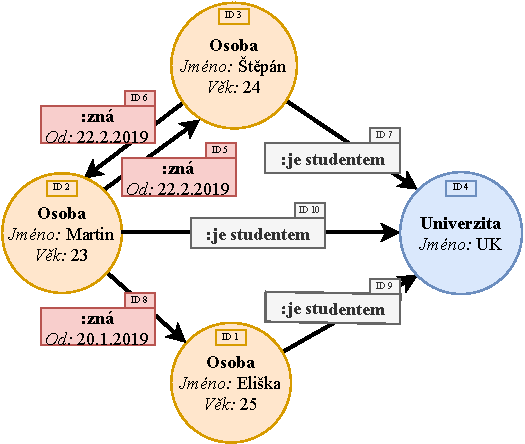
\includegraphics[width=100mm]{../img/propertyexample.pdf}\centering
\caption{Příklad Property grafu.}
\label{figure.propertygraphexample}
\end{figure}

Na obrázku \ref{figure.propertygraphexample} vidíme tři vrcholy se štítkem \textbf{Osoba}, které reprezentující fyzické osoby, a jeden vrchol se štítkem \textbf{Univerzita} reprezentující vysokou školu.
Štítku \textbf{Osoba} byly přiděleny dvě vlastnosti: \textit{Jméno} (řetězec) a \textbf{Věk} (číselná hodnota).
Štítku \textbf{Univerzita} byla přidělena jedna vlastnost: \textit{Jméno}, která odpovídá stejné vlastnosti štítku \textbf{Osoba} a mají stejný typ hodnoty (řetězec).
Mezi vrcholy fyzických osob existuje vztah \textbf{zná}, který určuje, zda jedna osoba (počáteční vrchol) zná druhou osobu (koncový vrchol).
Vlastnost \textit{Od} definuje datum, kdy došlo k poznání osoby.
Mezi vrcholy fyzických osob a vysokou školou existuje vztah \textbf{je studentem}, který říká, zda osoba studuje na dané vysoké škole.
Tento vztah nemá žádnou vlastnost.
Samotně pak každý element má přiřazeno \texttt{ID}.
Příklad vznikl na základě prvního grafu z dokumentace níže popisovaného PGQL.

V průběhu práce budeme graf splňující daný model označovat jako \textbf{Property graf}.

\section{Jazyk PGQL}
\label{req.pgql}

V naší práci budeme používat dotazovací jazyk PGQL \citep{pgql} verze 1.2 k dotazování nad Property grafem.
Jazyk je značné obsáhlý a k realizaci naší práce nepotřebujeme všechny jeho vlastnosti, proto jsme se rozhodli využít jeho podmnožinu.
V naší práci budeme pracovat jen s částmi \textit{Select}, \textit{Match}, \textit{Group by} a \textit{Order by}.
Ostatní části nebudeme používat.
V každém dotazu musí být vždy přítomná část \textit{Select} a \textit{Match}.
S částí \textit{Match} se pojí část \textit{From} specifikující název grafu, nad kterým se má vykonat dotaz.
Nicméně, v naší práci vždy budeme pracovat s jedním grafem, proto jsme část vyřadili. 
Zároveň v naší práci uvažujeme, že \textit{Order by} a \textit{Group by} nejsou zadány nikdy společně.

\begin{itemize}
\item \textit{Match:} definuje podgraf, který bude vyhledán v grafu.
Součástí definice podgrafu jsou proměnné, které jsou přístupné v ostatních částech dotazu.
Proměnná zde reprezentuje jeden element podgrafu.
Obecně existují dvě základní sémantiky vyhledávání \citep{graphmatch}: grafový izomorfismus a grafový homomorfismus (pro upřesnění odkazujeme na citovaný zdroj).
V naší práci budeme pracovat se sémantikou grafového homomorfismu, protože se jedná o obecnější pohled na vyhledávání.

\item \textit{Select:} určuje vrácená data ve formě tabulky jako u tabulkových databází.
K jednomu výsledku tak můžeme vrátit výčet informací.
Každá položka výčtu pak definuje jeden sloupeček tabulky.

\item \textit{Group by:} dovoluje seskupit výsledky dle zadaných klíčů a vypočítat agregační funkce pro výsledné skupiny.

\item \textit{Order by:} vykoná setřídění výsledků dle zadaných klíčů.
\end{itemize}

Nyní krátce popíšeme omezení a klíčové vlastnosti, s kterými budeme pracovat.
Pro komplexní popis odkazujeme na citovanou dokumentaci.

\subsubsection{Match}

Část \textit{Match} se skládá z posloupností elementů definující hledaný podgraf.
Posloupnosti jsou odděleny čárkou.
Položky v posloupnosti jsou vrcholy a hrany.
Položky vrcholů značíme pomocí \texttt{()} a položky hran pomocí šipek \texttt{->} (dopředná hrana), \texttt{<-} (zpětná hrana) a \texttt{-} (libovolná hrana).

Každé položce je možno přidělit jméno (definice proměnné) a predikát štítku.
Vrcholu přidělíme proměnnou vložením jména do kulatých závorek: \texttt{(jméno)}.
Hraně přidělíme proměnnou vložením jména do hranatých závorek: \texttt{-[jméno]->}, \texttt{<-[jméno]-} a \texttt{-[jméno]-}.
V části \textit{Match} musí být vždy přítomna alespoň jedna proměnná.
Pokud se v posloupnostech opakují proměnné znamená to, že v průběhu hledání musí dané položky obsahovat elementy se shodným \texttt{ID}.
Nicméně, proměnné hran se nesmí opakovat.
Pokud dvě posloupnosti nemají společnou proměnnou, tak výsledek je skalární součin daných posloupností. 

Predikát je vložen do závorek za jméno, pokud jméno chybí tak jen do závorek: \texttt{(jméno:štítek)}, \texttt{(:štítek)}, \texttt{-[jméno:štítek]->} a \texttt{-[:štítek]->}.
Predikát určuje výběr elementů pouze s daným štítkem.
Pokud se v posloupnostech opakuje proměnná se štítkem, pak štítek musejí mít i opakované definice proměnných.
Protože v našem modelu elementy mají pouze jeden štítek, tak element posloupnosti může mít pouze jeden predikát.
Navíc jsme vyřadili možnost aplikovat v predikátu operátor \texttt{|} (logická operace nebo), tj. nelze použít \texttt{(jméno:štítek|štítekDva)}.
Následují příklady \textit{Match} části na grafu z obrázku \ref{figure.propertygraphexample} (bez \textit{Select}) a uvedené výsledky hledání rovněž odpovídají danému obrázku:

\begin{enumerate}
\item
\begin{code}
match (x:Osoba) -> (y:Osoba)
\end{code}
Jsou zde dva vrcholy s názvy proměnných \texttt{x} a \texttt{y}.
Oba mají predikát štítku \texttt{:Osoba}.
To znamená, že do položek posloupnosti budou vybrány pouze elementy s daným štítkem.
Část \textit{Match} v průběhu hledání využívá pouze hrany vedoucí z proměnné \texttt{x}.
Výsledky hledání jsou dvojice vrcholů \texttt{x}-\texttt{y}: 2-1, 2-3, 3-2.
Hodnoty jsou zde \texttt{ID} elementů.

\item
\begin{code}
match (x:Osoba) <- (y:Osoba)
\end{code}
Část \textit{Match} v průběhu hledání využívá pouze hrany vedoucí do proměnné \texttt{x}.
Výsledky hledání jsou dvojice vrcholů \texttt{x}-\texttt{y}: 1-2, 2-3, 3-2.
Hodnoty jsou zde \texttt{ID} elementů.

\item
\begin{code}
match (x:Osoba), (x:Osoba) 
\end{code}
Zde vidíme dvě posloupnosti sdílející proměnnou \texttt{x}.
Protože první měla predikát, tak i druhé opakování musí mít stejný predikát.
Výsledky hledání jsou dvojice vrcholů \texttt{x}-\texttt{x}: 1-1, 2-2, 3-3.
Hodnoty jsou zde \texttt{ID} elementů.

\item
\begin{code}
match (x:Osoba), (y:Osoba) 
\end{code}
Zde vidíme dvě separátní posloupnosti bez sdílené proměnné, proto dojde ke vzniku skalárního součinu výsledků posloupností.
Výsledky hledání jsou dvojice vrcholů \texttt{x}-\texttt{y}: 1-1, 1-2, 1-3, 2-1, 2-2, 2-3, 3-1, 3-2, 3-3.
Hodnoty jsou zde \texttt{ID} elementů.

\end{enumerate}

\subsubsection{Výrazy}

Zbylé části se skládají převážně z výrazů (např. \texttt{select x, y ...}, kde \texttt{x} a \texttt{y} jsou funkce vracející \texttt{ID} elementů).
Samotné výrazy v jazyku PGQL mohou být značně komplikované, proto jsme vybrali tři základní výrazy, které budeme využívat.
\begin{itemize}

\item Funkce vracející \texttt{ID} elementu. 
V dotazu se reprezentuje použitím názvu proměnné.
Lze zadat v jakékoliv části kromě \textit{Match}.
Například:
\begin{code}
select x, y match (x) -> (y)
\end{code}
Dotaz obsahuje dva výrazy \texttt{x} a \texttt{y} v části \textit{Select}.
\textit{Select} část vytváří tabulku se dvěma sloupečky \texttt{x} a \texttt{y}, které obsahují \texttt{ID} elementů v daných proměnných.

\item 
Přístup k hodnotě vlastnosti elementu.
Lze zadat v jakékoliv části kromě \textit{Match}.
V dotazu se reprezentuje použitím názvu proměnné s názvem vlastnosti sloučených pomocí tečky.
Například: 
\begin{code}
select x.VlastnostJedna, y.VlastnostDva match (x) -> (y)
\end{code}
Dotaz obsahuje dva výrazy \texttt{x.VlastnostJedna} a \texttt{y.VlastnostDva} v části \textit{Select}.
\textit{Select} část vytváří tabulku se dvěma sloupečky \texttt{x.VlastnostJedna} a \texttt{y.VlastnostDva}, které obsahují hodnoty vlastností elementů v daných proměnných.
Tento výraz se například nemusí povést vyhodnotit, protože vlastnost nemusí existovat na daném elementu.
V takovém případě budeme předpokládat, že výraz vrací nějakou konstantu definující selhání výpočtu.

\item 
Agregační funkce, které vypočítají výslednou hodnotu pro skupiny vytvořených při seskupování (\textit{Group by}).
Pokud nebylo zadáno \textit{Group by} a je použita agregační funkce, pak ve zbylých částech kromě \textit{Match} mohou být pouze agregační funkce.
V takovém případě všechny výsledky patří do jedné skupiny.
Agregační funkce povolíme pouze v části \textit{Select}, protože \textit{Order by} a \textit{Group by} nemůžou být nikdy zadány společně.
Nedovolíme rekurzivní používání daných funkcí, tj. agregační funkce nemůže mít na vstupu další agregační funkci.
Funkce na vstupu mají hodnotu vypočteného výrazu (tj.~\texttt{ID} nebo přístup k vlastnosti).
Musíme brát v potaz, že při výpočtu výrazu může dojít k selhání a tedy funkce musí umět pracovat s konstantou definující selhání výpočtu.
PGQL definuje pět funkcí:
\begin{enumerate}
\item Funkce minima vracející minimum z hodnot na vstupu. 
\\*Značená \texttt{min(...)}.
Pracuje s číselnými typy i řetězci.
\item Funkce maxima vracející maximum z hodnot na vstupu. 
\\*Značená \texttt{max(...)}.
Pracuje s číselnými typy i řetězci.
\item Funkce aritmetického průměru vracející aritmetický průměr hodnot na vstupu.
Značená \texttt{avg(...)}.
Pracuje pouze s číselnými typy.
\item Funkce součtu vracející součet hodnot na vstupu. Značená \texttt{sum(...)}.
Pracuje pouze s číselnými typy.
\item Funkce počtu vracející počet prvků na vstupu, značená \texttt{count(...)}.
Pracuje s číselnými typy i řetězci.
Funkce má dva módy.
První mód je použití zápisu \texttt{count(výraz)}, kde \texttt{výraz} je přístup k \texttt{ID} nebo vlastnosti elementu.
Druhý mód je použití zápisu \texttt{count(*)}.
Tento zápis nepotřebuje vyhodnotit výrazy.
Pokud byl například zadán dotaz:
\texttt{select count(*) match (x)}, pak v tomto dotaze nepotřebujeme znát elementy z části \textit{Match}, ale stačí nám jejich počet.
\end{enumerate}
\end{itemize}

\subsubsection{Select}

\textit{Select} část může obsahovat pouze výše zmíněné výrazy oddělené čárkami.
V~této části lze přistoupit k proměnným, které jsou definované v \textit{Match} části, nebo zadat výrazy agregačních funkcí.
Výsledkem části \textit{Select} je tabulka.
Sloupečky v~tabulce představují výrazy zadané v dané části.
Řádky tabulky jsou pak hodnoty výrazů pro výsledky z části \textit{Match} nebo \textit{Group/Order by}.
Existuje ještě speciální operátor \texttt{*}, který lze zadat pouze v případě, pokud je v~dotazu jen část \textit{Select} a \textit{Match}.
V takovém případě se \texttt{*} nahradí všemi proměnnými z části \textit{Match}.
Následují příklady použití \textit{Select} části:
\begin{itemize}
\item
Použití obyčejných výrazů:
\begin{code}
select x, y, x.Vlastnost match (x) -> (y)
\end{code}
Dojde k návratu tabulky se třemi sloupečky.
Sloupečky obsahují hodnoty daných výrazů.

\item
Použití operátoru \texttt{*}:
\begin{code}
select * match (x) -> (y)
select x, y match (x) -> (y) 
// dotazy jsou ekvivalentní
\end{code} 

\item
Použití agregačních funkcí v \textit{Select} bez části \textit{Group by}:
\begin{code}
select min(x.Vlastnost), avg(x.Vlastnost) match (x) -> (y)
\end{code}
V takovém případě je výsledkem dotazu pouze jedna dvojice výsledných hodnot dvou funkcí, protože všechny výsledky jsou seskupeny do jedné skupiny.
Část \textit{Select} zde tedy může zadávat pouze agregační funkce.

\item
Použití části \textit{Select} zároveň s částí \textit{Group by}:
\begin{code}
select avg(x.Vlastnost), x match (x) -> (y) group by x
\end{code}
Část \textit{Select} může obsahovat pouze výrazy agregačních funkcí nebo výrazy zadaných v části \textit{Group by}.
Výše zmíněný dotaz bez výrazu \texttt{x} v \textit{Select} části a ponecháním pouze agregační funkce je správně.
Rovněž odstraněním agregační funkce z \textit{Select} části a zanecháním pouze druhého výrazu je správně.
Výsledná tabulka má počet řádků rovný počtu vytvořených skupin.
\end{itemize}

\subsubsection{Order by}

\textit{Order by} definuje klíče (výrazy), podle kterých budou výsledky z části \textit{Match} setříděny.
\textit{Order by} může přistupovat pouze k proměnným z \textit{Match} části.
\textit{Order by} a \textit{Select} části nemusí mít shodné výrazy.
Výrazy v této části jsou opět odděleny čárkami.
Operátor \texttt{asc}/\texttt{desc} za výrazem definuje, zda jsou hodnoty tříděny vzestupně/sestupně.
Pokud operátor chybí, tak je jako výchozí operátor použit \texttt{asc}.
Následují příklady použití \textit{Order by} části:
\begin{itemize}
\item
Použití jednoho klíče:
\begin{code}
select x, y match (x) -> (y) order by x
\end{code}
Výsledky z \textit{Match} jsou setříděny podle hodnot \texttt{x} vzestupně.

\item
Použití dvou klíčů:
\begin{code}
select x, y match (x) -> (y) order by x, y
\end{code}
Výsledky z části \textit{Match} jsou setříděny podle hodnot \texttt{x} vzestupně.
Pokud se dva výsledky shodují v dané hodnotě, pak je použito porovnání hodnotou \texttt{y}.
Obecně se aplikuje stejný postup, pokud je tříděno podle více než dvou klíčů.

\item
Použití operátoru \texttt{desc}:
\begin{code}
select x, y match (x) -> (y) order by x desc
\end{code}
Výsledky z části \textit{Match} jsou setříděny podle hodnot \texttt{x} sestupně.
\end{itemize}

\subsubsection{Group by}

\textit{Group by} definuje klíče seskupení (výrazy).
Výsledkem \textit{Group by} je množina skupin.
Skupiny obsahují výsledky prohledávání z části \textit{Match}.
Všechny výsledky v jedné skupině mají stejné hodnoty klíčů seskupení. 
Výrazy jsou odděleny čárkami.
\textit{Select} část může obsahovat výrazy agregačních funkcí a výrazy klíčů seskupení.
Agregační funkce se vypočítají pro každou skupinu zvlášť.
Pokud není zadána část \textit{Group by} a dotaz obsahuje výrazy agregačních funkcí, pak se jedná o seskupení všech výsledků do jedné skupiny.
Následují příklady použití \textit{Group by} části:
\begin{itemize}
\item
Použití jednoho klíče:
\begin{code}
select x match (x) -> (y) group by x
\end{code}
Výsledky z části \textit{Match} jsou seskupeny podle hodnot \texttt{x}.

\item
Použití dvou klíčů:
\begin{code}
select x, y match (x) -> (y) group by x, y
\end{code}
Výsledky z části \textit{Match} jsou seskupeny dle uspořádané dvojice (\texttt{x}, \texttt{y}).
Pokud obecně existuje více klíčů, pak jsou seskupeny dle uspořádané \textit{n}-tice.
\end{itemize}


\chapter{Analýza}

V této kapitole se pokusíme analyzovat problémy výstavby a úpravy dotazovacího enginu dle zadání práce.
Zároveň poskytneme možná řešení daných problémů.
Budeme zde postupovat v několika krocích. 
Začneme obecným návrhem dotazovacího enginu a projdeme hlavní koncepty pro implementaci.
V druhém kroku zvážíme kroky vykonávání dotazů a postup výběru řešení částí Order by a Group by, které se budou vykonávat po dokončení vyhledávání dotazu.
V třetím kroku provedeme analýzu úprav pro agregaci v průběhu vyhledávání. 
Součástí této části bude analýza algoritmů Order by a Group by pro dané úpravy. 

\section{Obecný pohled na engine}

V naší představě je dotazovací engine určen pro práci nad grafem, který je celý obsažen v paměti, včetně vlastností elementů grafu.
Graf bude načten v definovém formátu a následně na něm budou vykonávány dotazy.
V momentě načtění graf bude pouze statický, tedy nebude docházet k žádným změnám.
Nad grafem se pak vykoná uživatelsky definovaný dotaz.
Dané omezení jsme zvolili, protože hlavním cílem je testovat pouze části Group by a Order by.
Vytvořit reálnou grafovou databázi by zabralo netriviální časové období.

Při obecném pohledu na engine jsme lokalizovali hlavní bloky výstavby, které musíme uvážit.
Jsou to: reprezentace grafu, parsování uživatelského dotazu, výrazy (expressions) a dotaz/vykonání dotazu.
Graf nám bude simulovat grafovou databázi. 
Samotně pak určuje formát objektů, nad kterými je vykonán uživatelský dotaz.
Při parsování se načítá uživatelký dotaz do interní reprezentace.
Expressions slouží k výpočtu hodnot z uživatelsky zadaných výrazů.
Například v části order by x.PropOne, musíme vědět, jak reprezentovat výraz x.PropOne a získat jeho hodnotu. 
Na základě interní reprezentace se musí vytvořit struktury dotazu a definovat exekuční plán. 
Z obecných úkonů částí vidíme, že se nejedná o stand-alone části.
Vytváří se nám závislosti, které budeme muset uvážit.

\section{Reprezentace grafu} \label{anal.grafrep}

Musíme uvážit, jak reprezentovat graf.
Graf bude simulovat grafovou databázi.
Z části \ref{requirements} jsou hlavními faktory námi zvolená podmnožina jazyku PGQL a že se jedná o Property graf.
Pro případy nejednoznačnosti označíme \verb+elType+ jako typ elementu v Property grafu a \verb+propType+ jako typ vlastnosti.

\subsection{Elementy grafu a jejich typ}

Musíme zvažovat reprezentaci elementů grafu a jejich \verb+elType+.
V našem případě jsou elementy pouze vrcholy a orientované hrany.
\verb+elType+ definuje seznam vlastností na elementu. 
Vlastnosti jsou také typované.
Vrchol a hrana musí mít rozdílný \verb+elType+, ale samotné vlastnosti se mohou opakovat pro oba druhy elementů.
Každá hodnota vlastnosti musí být přístupná skrze daný element:

\begin{itemize}

\item Pokud držíme element grafu, musíme být schopni jej rozlišit od ostatních elementů.

\item Pokud držíme element grafu, musíme být schopni přistoupit k hodnotám jeho vlastností.

\end{itemize}

V naší představě je řešení následovné.
Elementy budou třídy.
Každý element grafu bude potomkem jednoho abstraktního předka a potomci si budou definovat svá specifika.
Potomek bude vrchol a hrana.
Předek si bude pamatovat unikátní \verb+ID+, abychom elementy dokázali rozlišit. 
Předek navíc bude znát svůj \verb+elType+. 
Bude se jednat o ukazatel na třídu.
Daná třída by reprezentovala pouze jeden \verb+elType+ a bude společná všem elementům majících daný \verb+elType+.
V třídě by byl obsažen seznam \verb+IDs+ elementů daného typu, jejich pořadí (např: dle vkládání do seznamu) a vlastností v podobě polí s hodnotami.
Vlastnost musí být přístupná skrze mapu/slovník, protože může nastat situace, kdy daná vlastnost na elementu neexistuje. 
Pro náš případ nebudeme uvažovat situaci, kdy vlastnost pro nějaký element nemá definovanou hodnotu.
Vlastnosti tedy budou přístupné pomocí unikátního identifikátoru pro celý graf.
Hodnoty vlastností každého elementu by ležely na pozicích dle pořadí \verb+IDs+.
Nyní, pokud držíme element grafu, můžeme přistoupit k hodnotě vlastnosti skrze tabulku pomocí jeho \verb+ID+.    
Samotný přistup pak může být realizován například generickou funkcí. 

\subsection{Struktury obsahující elementy}

Nyní musíme analyzovat jaké struktury by byly idální pro uchovávání elementů grafu.
Musíme brát v potaz, že propojení mezi vrcholy pomocí hran přímo ovlivňuje vyhledávání v části Match.
V průběhu vyhledávání v určitý moment vždy držíme odkaz na nějaký element grafu.
Na základě daného elementu musíme provést akci:

\begin{itemize}

\item Pokud držíme vrchol, musíme být schopni přistoupit k jeho hranám. Hranám z/do něj. Daný přístup by měl být co nejrychlejší a neměl by obsahovat žádné iterace. V průběhu hledání se z vrcholu musí projít skrze všechny jeho hrany. Ideálně by měly být hrany přístupné skrze index.

\item Pokud držíme hranu, musíme být schopni přistoupit ke koncovému vrcholu. V průběhu hledání vždy vlastníme vrchol než přistoupíme k jeho hraně a následně k jejímu koncovému vrcholu. Tímto můžeme vyloučit nutnost, aby hrana znala informaci o svém původu.

\item Pokud držíme element grafu, chceme být schopni přistoupit k jeho sousedním elementů v obsajující struktuře za předpokladu, že víme, jestli se jedná o hranu nebo vrchol. 

\end{itemize}

K vyřešení daných problému v naší představě bychom použili tři pole.
Pole vrcholů, pole out hran a in hran. 
Zde by bylo vhodné vytvořit nové potomky obecné hrany: out hrana a in hrana.
Hrany by si pamatovali svůj koncový vrchol.
Pro in hranu by to byl vrchol odkud vychází, aby bylo možné v moment držení vrcholu projít skrze ni na vrchol další.
Každé pole tedy bude mít unikátní typ, který nám pomůže rozlišit k jaké situaci má dojít v průběhu prohledávání.
Abstraktní předek všech elementů by si měl nově pamatovat i svou pozici v daných polích pro rychlý přístup k jeho sousedům.

Zbývá vyřešit vztah hran a vrcholů.
Řešení, které bychom chtěli zvolit, je mít hrany v polích seskupeny podle: vrcholů odkud vycházejí (pole out hran), vrcholů kam směřují (pole in hran).
Vrchol by si pak pamatoval rozsah svých hran v příslušných polích. 
Chceme-li procházet hrany vrcholu, stačí procházet pole out/in hran pomocí rozsahů uložených v daném vrcholu.
Tedy čtyř indexů.
Skrze indexy můžeme pak pole libovolně iterovat.

Uvažovali jsme nad různými alternativami. 
Mít jeden typ hrany obsahující všechny nutné informace.
Řešení je paměťově přijatelnější, ale nastává problém s přístupem k in hranám vrcholu.
Řešením by mohlo být vytvořit pole in/out hran pro každý vrchol. 
Daný přístup nám případá výrazně náročnější z hlediska paměti, protože musíme vytvářet pole pro každý vrchol zvlášť. 

\subsection{Návrh vstupních grafových dat} \label{anal.vstup}

Vstupní soubory musí obsahovat informace nutné pro Property graf.
Budeme očekávat dva druhy souborů.
Soubory schémat typů elementů a jejich vlastností.
Datové soubory pak budou obsahovat konkrétní data elementů.
(Jedná se o návrh a finální specifikaci uvedeme v rámci implementace.)

Protože každý element grafu má svůj \verb+elType+, budeme mít na vstupu dva soubory schémat pro hrany a vrcholy.
Schéma bude obsahovat informace o všech \verb+elType+ a \verb+propType+ vyskytujících se v grafu.
Pro \verb+elType+ je důležitý název a výčet vlastností.
Vlastnosti pak musí nést svůj název a \verb+propType+.
Vidíme, že se jedná jen o výčet \verb+(name/value)+ dvojic (např. \verb+(PropertyOne, integer)+).
V tomto případě se nám jeví nejvhodnější zvolit pro reprezentaci schémat formát JSON.
\verb+elType+ bude reprezentován JSON objektem. 
Bude obsahovat položku \verb+Kind+, jejíž hodnota udává jméno \verb+elType+.
Za ní bude následovat výčet vlastností.
Vlastnosti budou reprezentovány dvojicí \verb+(propName/propType)+.
Záznamy pak budou obsaženy v JSON poli:
\begin{code}
Soubor schéma vrcholů:
[    { "Kind": "BasicNode" }, 
     { "Kind": "BasicNodeTwo", "PropertyOne": "integer" } ]
Soubor schéma hran:"
[    { "Kind": "BasicEdge" }, 
     { "Kind": "BasicEdgeTwo", "PropertyOne": "integer" } ]
\end{code}
Jako určující \verb+propTypes+ pro náš případ enginu bychom chtěli zvolit dva druhy.
První by byla číselná hodnota značená integer (32-bit integer).
Další by představoval řetězec značený string.
Práce s řetězci je obecný problém a existuje mnoho znakových sad, proto bychom chtěli zvolit vstupní řetězce pouze se znaky ASCII.  
Dané dva druhy představují základní typy použitých v komerčních sférách.

Samotná data budou obsažena opět ve dvou separatních souborech pro hrany a vrcholy.
Chtěli bychom reprezentovat konkrétní data pomocí jednoduchého .csv souboru.
Každý řádek reprezentuje jednu hranu/vrchol.
V první řadě řádek musí obsahovat unikatní \verb+ID+ elementu a jeho \verb+elType+. 
Za \verb+elType+ následuje seznam hodnot vlastností v pořadí určených schématem.
Pro hrany existuje na řádku navíc záznam \verb+ID+ vrcholů, které spojuje.
Oddělovače mezi daty jsou implementační detail.
Pro naše účely se jedná o dostačující formát a poskytuje nám jednoduché možnosti parsování.
Pokud by docházelo v budoucnu k rozšířením, například více slovné vlastnosti nebo XML vlastnosti, musí dojít k úpravě daných formátů.

Pro výše zmíněné schéma by datové soubory mohly vypadat následovně:
\begin{code}
Soubor hran:
ID elType fromID toID Properties // bez této hlavičky
50 BasicEdge 0 0 
51 BasicEdgeTwo 0 1 44
...
Soubor vrcholů:
ID elType Properties // bez této hlavičky
0 BasicNode
1 BasicNodeTwo 42
...
\end{code}

\bigskip
\textit{Analyzovali a navrhli jsme způsob reprezentace grafu společně s formátem datových souborů.
Samotné načítání je už implementační detail.
Nyní musíme analyzovat způsob získání informací z uživatelem zadaného dotazu. }

\section{Parsování uživatelského dotazu}

Uživatelský dotaz se pohybuje v rozsahu definovaném v sekci PGQL \ref{req.pgql}.
Nicméně, je zde nutné přemýšlet i nad možnými rozšířeními.
Například může dojít k přidaní částí Where a Having spolu s nutností porovnávání (Where x.PropOne $\leq 10$).
Proto se budeme snažit držet základních principů object oriented programming a volit vhodné návrhové vzory.

K načtení uživatelského dotazu se nám jeví jako nejvhodnější způsob použít techniky známé z překladačů programovacích jazyků.
Budeme vycházet ze základních principů knihy o překladačích \citep{dragoonBook}.
V prvním kroku dojde k lexikální analýze uživatelsky zadaného řetězce.
Dojde k vytvoření tokenů.
V druhém kroku dojde k syntaktické a semantické analýze tokenů.
Metodou top-down parsing \citep[str. 217]{dragoonBook} se vytvoří stromová struktura reprezentující daný dotaz.
Poslední krok provede vytvoření tříd reprezentující dotaz pomocí iterace stromové struktury.
Iterace a sběr dat ze stromové struktury budou implementovány návrhovým vzorem Visitor \citep[str. 331]{patterns}.
V naši představě bychom chtěli vygenerovat stromovou strukturu pro každou hlavní část dotazu (Match, Select, Order by a Group by).
Nyní bychom mohli sestavit Visitor pro každou část separatně a vyřadit tak nutnost jednoho globálnáho Visitoru.
Dané postupy nám pak umožní jednoduše pracovat s naší podmnožinou jazyka PGQL (sekce \ref{req.pgql}).


\subsection{Match a proměnné} \label{anal.mathcandvar}

Každá hlavní část dotazu po sesbírání informací pomocí Visitoru vygeneruje určité struktury.
Pro Match se přímočaře naskytuje reprezentovat posloupnosti vrcholů a hran pomocí polí.
Každá posloupnost oddělená čárkou bude obsažena v samostatném poli.
Pole bude obsahovat třídy.
Třída si musí pamatovat jakou proměnou reprezentuje, \verb+elType+ pokud je definován a jde-li o hranu (in/out/any) nebo vrchol.
Jedná se o všechny nutné informace, které můžeme následně využít k vytvoření vzoru prohledávání grafu.
Všimout si musíme faktu, že Match část definuje proměnné ve zbytku dotazu.
Během parsování musíme určit zda se jedná o validní proměnnou a při vypočtech hodnot výrazů je nutné vědět přesně k jaké proměnné musíme přistoupit.
Problém se dá řešit vytvořením mapy/slovníku přistupných proměnných pro zbytek dotazu.
Proměnným pak můžeme přiřadit \verb+ID+.

\subsection{Select, Order/Group by}

Ostatní části Group by, Order by a Select obsahují výrazy proměnných (např: order by x), přístup k vlastnostem proměnných (např: select x.PropOne) nebo volání agregačních funkcí (\verb+min+, \verb+max+, \verb+avg+, \verb+sum+ a \verb+count+).
Proměnné zde představují elementy grafu.
Várazy se však musí evaluovat za běhu programu.
Dalším problémem je, že výrazy mají různorodé návratové hodnoty.
Výraz x (\verb+ID+ vrcholu) lze chápat jako integer.
Váraz x.PropOne má návratovou hodnotu dle \verb+propType+, který je definovám ve vstupním schématu.
Agregační funkce \verb+min+, \verb+max+ mají návratovou hodnotu definovanou na základě jejich vstupních argumentů.
Funkce \verb+sum+ a \verb+count+ by měli ideálně pracovat s typem, který by předešel přetečení.
U \verb+avg+ se očekává hodnota s desetinnou čárkou.  
V budoucnu však může dojít k rozšířením a vyvstanou složitější výrazy, například infixová notace x.PropOne + y.PropOne nebo zmiňované porovnání z Where/Having části.
Problém nám usnadňuje fakt, že vlastnosti nesoucí stejné jméno mají stejný \verb+propType+.
Pokud ne, je nutné určit vhodnou návratovou hodnotu.
Navíc musíme brát v potaz, že daný výraz se nemusí vyhodnotit, například absence vlastnost na vrcholu.
Proto jsme byli nuceni vymyslet systém výrazů (expressions).

\subsection{Expressions} \label{anal.expressions}

Systém vytváření a vyhodnocování výrazů efektivně za běhu je obecně složitý problém.
Omezíme se pouze na případy: přístup k proměnné, přístup k hodnotě vlastnosti proměnné a agregační funkce (\verb+min+, \verb+max+, \verb+avg+, \verb+sum+ a \verb+count+).

Základní myšlenka je reprezentovat výraz pomocí stromové struktury. 
Každý vrchol stromové struktury bude reprezentovat určitou akci.
Vrcholy budou výše vypsané výrazy. 
Na struktuře bude existovat metoda pro vyhodnocení.
Její návratová hodnota bude dvojice úspěch vyhodnocení + vypočtená hodnota. 
Dané struktury musí být read-only, protože se budou využívat v paralelním prostřední.
Metody by se mohli libovolně dodávat při nutnosti použití nových struktur. 

Následuje ukázka možného kódu v jazyce C\#:
\begin{code}
// Základní rodičovské třídy
abstract class Expression { }
abstract class ExpressionReturnValue<T>: Expression {
  public abstract bool TryEvaluate(Element[] elms, out T retVal); 
}
abstract class VariableAccess<T>: ExpressionReturnValue<T> {
     readonly int accessedVariableID; }
\end{code}
Třída reprezentující přístup k \verb+ID+ proměnné:
\begin{code}
class VariableIDAccess: VariableAccess<int> {
  public override bool TryEvaluate(Element[] elms, out int retVal) {
     returnValue = elms[accessedVariableID].ID;
     return true; 
  }
}
\end{code}
Třída \verb+VariableAccess+ nám poskytuje abstrakci pro přístup k proměnné.
Položka \verb+accessedVariableID+ určuje k jaké proměnné se má přistoupit.
Zde předpokládáme, že pole \verb+Element[]+ obsahuje proměnné přesně v pořadí, jak se vyskytly v části Match.
Tedy pokud je roven Match (x) -> (y), tak jeden výsledek hledání by bylo pole obsahující dva elementy x a y.
Jedná se pouze o ilustrační příklad. 

Případ přístupu k vlasnosti by mohl vypadat následovně:
\begin{code}
class VariablePropertyAccess<T>: VariableAccess<T> {
  reaonly int accessedPropertyID; 
  public override bool TryEvaluate(Element[] elms, out T retVal) {
    return elms[accessedVariableID].
               GetPropertyValue<T>(accessedPropertyID, out retVal);
  }
}
\end{code}
Zde dojde k volání metody na elementu grafu, který přistoupí k třidě reprezentující jeho \verb+elType+.
Třída pak na základě existence vlastnosti vrátí hodnotu nebo neuspěje.
Timto dokážeme vyřešit základní definované problémy.

Zbává uvažovat, jakým způsobem reprezentovat agregační funkce.
Agregační funkce představují několik problémů.
Funkce je vypočtená pouze pro skupiny. 
Skupiny jsou vytvářeny v části Group by.
Jejich návratové hodnoty jsou finální pouze po dokončení Group by. 
Vstupem funkcí je výstupní hodnota uživatelem zadané expression.
Argument, dle kterého se aktualizuje agregovaná hodnota, je nutný znát pouze v době vykonání Group by.
Dle naši představy je ideální vytvořit dva separátní koncepty.
První koncept bude zahrnovat výpočet hodnot argumentu společně s logikou agregační funkce.
Koncept bude reprezentován třídou, která vlastní stromovou strukturu dle předchozího příkladu.
Zároveň bude obsahovat logiku počítané funkce.
Například logika funkce \verb+min+ je porovnat dvě hodnoty a vybrat menší.
Na vstupu dané funkce pak bude úložiště hodnoty dané skupiny.
Všechny počítané agregační funkce zadané uživatelem označíme pomocí \verb+ID+.
Druhý koncept představuje nový potomek třídy expression.
Daný potomek si pamatuje \verb+ID+ přistupované agregační funkce a na vstupu očekává strukturu reprezentující skupinu.
K hodnotě počítané agregace přistoupíme pomocí její \verb+ID+.

Následuje ukázka druhého konceptu:
\begin{code}
class GroupAggValueAccess<T>: ExpressionReturnValue<T> {
  reaonly int accessedAggregationFuncID; 
  public override bool TryEvaluate(Group group, out T retVal) {
    retVal = group.GetAggValue<T>(accessedAggregationFuncID);
    return true; }}
\end{code}
\verb+Group+ reprezentuje výsledky jedné skupiny.
\verb+accessedAggregationFuncID+ je \verb+ID+ vypočítané agregační funkce.
Hodnota funkce se vrací pomocí \verb+GetAggValue<T>+.

Následuje ukázka prvního konceptu:
\begin{code}
abstract class Aggregation { }
abstract class Aggregation<T>: Aggregation {
  public ExpressionReturnValue<T> expr; // Argument of the agg. func.
  public abstract void Apply(ValueStorage storage, Element[] elms);
}

public class Sum<T>: Aggregation<T>{
  public override void Apply(ValueStorage storage, Element[] elms) {
    if (expr.TryEvaluate(elms, out T retVal)) {
      storage.value += retVal;
    }
  }
}
\end{code}
Zde vidíme položku \verb+expr+, která reprezentuje vstupní expression agregační funkce.
Funkce \verb+Apply+ je logikou funkce. 
Vidíme funkci \verb+Sum+. 
Logikou je přičtení vypočítané hodnoty do poskytnutého úložište, pokud dojde k úspěšné evaluaci výrazu.
Pomocí našeho návrhu pak můžeme vyřešit i budoucí rozšířešení, jako třeba aritmetické operátory nebo porovnání.

Třídy pro binární sčítání mohou vypadat takto:
\begin{code}
class ExpressionBinOperation<T>: ExpressionReturnValue<T> {
  public ExpressionReturnValue<T> expr1;
  public ExpressionReturnValue<T> expr2;
}

class ExpressionIntegerAdd: ExpressionBinOperation<int>{
  public override bool TryEvaluate(Element[] elms, out int retVal) {
    if (expr1.TryEvaluate(elms, out int expr1Val) &&
        expr2.TryEvaluate(elms, out int expr2Val)) {
      retVal = expr1Val + expr2Val;
      return true;
    } else {
      retVal = default;
      return false;
    }
  }
}
\end{code}
Zde \texttt{ExpressionIntegerAdd} rozšiřuje obecný binární operátor a určuje návratovou hodnotu výrazu.
V těle funkce \texttt{TryEvaluate} dojde k pokusu o vyhodnocení dvou podvýrazů.
Při úspěchu dojde k vypočtení finální hodnoty a v opačném případě dojde k selhání vyhodnocení. 

\bigskip
\textit{Tímto jsme vyřešeli problémy parsování a reprezentace expressions pro náš engine.
Kód je pouze ilustrační a není finální.
Použili jsme jej, protože poskytoval lepší možnosti vysvětlení konceptu než obrázek.
Nyní přistoupíme k problémům vykonávání dotazu.}

\clearpage

\section{Vykonání dotazu} \label{anal.vykonanidotazu}

Máme připravené obecné podklady.
Víme jak reprezentovat graf a jak budeme získávat informace z uživatelem zadaného dotazu.
Dotaz bude vykonán nad naší reprezentací grafu.
Abychom splnili zadání, tak Group/Order by musí být vykonány po dokončení vyhledávání vzoru.
Vylepšená řešení budou dané části vykonávat v průběhu vyhledávání.
V ideálním případě chceme dosáhnout toho, aby dotazovací engine poskytoval dva módy.
Mód zde reprezentuje způsob vykonání dotazu.
Uživatel enginu si při spuštění vybere chtěný mód.
Tudíž, módy musí v programu koexistovat.
V této části analyzujeme obecný model vykonání, který posléze v sekci \ref{anal.improvement} upravíme, aby vykonával Group/Order by v průběhu hledání.

Při zkoumání vlastností hlavních částí PGQL (sekce \ref{req.pgql}) jsme si uvědomili jejich separaci logiky z hlediska vykonávání dotazu.
Match prohledává graf a produkuje výsledky. 
Select výsledky vypisuje. 
Order/Group by třídí/seskupuje vyprodukované výsledky.
Filtrace výsledků je prováděna v části Where a Having.
Tedy dané části se mohou vyvíjet nezávisle na sobě a následně propojit dle priorit.

Priority (zleva největší):
\begin{code}
      Match > Where > Group by > Having > Order by > Select 
\end{code}
Match vyprodukuje výsledky, Where je profiltruje, Group by je seskupí, Having opět profiltruje, následně jsou setříděny a jako poslední krok se provede výpis uživateli.
Propojení pak tvoří primitivní exekuční plán.
Při podrobnějším zkoumání jsme zjistili, že dané schéma značně připomíná návrhový vzor Pipes and Filters \citep[str. 53]{patterns2}.
Ačkoliv v naší práci použitá podmnožina PGQL (sekce \ref{req.pgql}) neobsahuje Having a Where, jsme si vědomi provázanosti částí Match/Where a Group by/Having.
Pokud by byli v budoucnu doimplementovány, tak mohou být propojeny pro docílení lepší výkonnosti. 

Poznatky jsme se rozhodli aplikovat v našem návrhu.
Každá část dotazu bude reprezentována objektem (obrázek \ref{figure.diaQueryObjects}).
Metoda \verb+Compute+ implementuje logiku objektu.
Propojení se realizuje pomocí položky \verb+next+.
Dle uživatelského dotazu se vytvoří objekty a propojí dle priorit výše (obrázek \ref{figure.diaQueryObjectsCon}).
Propojejí bude realizováno od nejmenší po největší, protože práce s nejvyšší prioritou je vykonána první a po dokončení její práce ji už nepotřebujeme.
Tedy můžeme uvólnit její zdroje.
Při vykonání se provede rekurzivní voláni pro vyhodnocení objektů v položce \verb+next+ (obrázek \ref{figure.diaQueryObjectsCall}). 

\begin{figure}[!htp]
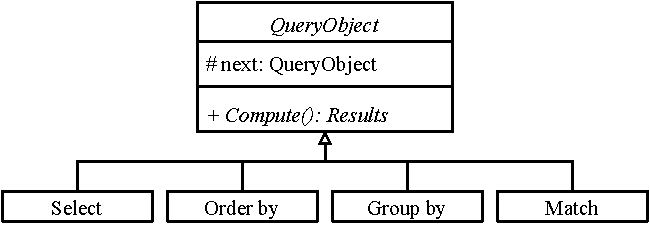
\includegraphics{../img/diaQueryObjects.pdf}\centering
\caption{UML class diagram objektů představující části dotazu.}
\label{figure.diaQueryObjects}
\end{figure}

\clearpage

\begin{figure}[!htp]
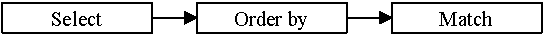
\includegraphics{../img/diaQueryObjectsCon.pdf}\centering
\caption{Propojení objektů pomocí položky \texttt{next} pro dotaz select x match (x) order by x.}
\label{figure.diaQueryObjectsCon}
\end{figure}

\begin{figure}[!htp]
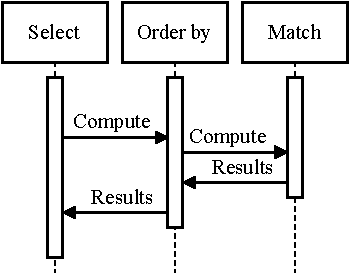
\includegraphics{../img/diaQueryObjectsCall.pdf}\centering
\caption{UML activity diagram rekurzivního volání metody \texttt{Compute} pro dotaz select x match (x) order by x.}
\label{figure.diaQueryObjectsCall}
\end{figure}

\subsection{Paralelizace vykonání dotazu}

Poslední věc nutnou ošetřit je způsob paralelizace dotazu.
Existuje několik možností.
Paralelizace bude provedena pouze interně pro každy objekt nebo dojde k vypracování složitějšího modelu.
V naší představě bychom volili první variantu.
Pomocí ní zaručíme nezávislost objektů a nebudeme nutni vytvářet závislosti mezi objekty.
Při analýze jednotlivých částí budeme vycházet z předpokladu, že existuje \texttt{ThreadPool} vláken.
Do \texttt{ThreadPool} budeme zařazovat úkony k vykonání (\texttt{Tasks}).

\subsection{Formát výsledků} \label{anal.tables}

Mezi částmi dochází k předávání výsledků.
Výsledky musí mít definovaný formát, aby každá část dokázala správně provádět svou logiku.
V části Match dochází ke generování obecných výsledků.
V části Group by dojde k vytvoření skupin a výpočtů agregačních funkcí.
Pokud je v uživatelském dotazu zahrnuto Group by, tak zbylé části musí očekávat jiný formát výsledků.
Daný formát musí obsahovat skupiny a výsledné hodnoty agregačních funkcí.

Obecné výsledky hledání budeme ukládat do tabulky.
Jeden řádek tabulky bude reprezentovat jeden výsledek hledání.
Nyní musíme rozhodnout, jaké informace do tabulky uložíme.
V části Match se pracuje s elementy grafu.
Jeden výsledek hledání obsahuje seznam elementů, které odpovídají vzoru.
Máme dvě možnosti, jak daný výsledek zpracovat.
První varianta v části Match při jeho nalezení vypočte hodnoty všech výrazů obsažených ve zbytku dotazu.
Sloupeček představuje hodnoty jednoho výrazu.
Tato varianta nám nepřišla vhodná, protože by objekt Match musel znát informace o výrazech v celém dotazu.
Navíc výrazy v částech mohou být rozdílné.
Tedy se vytváří nutnost vytvářet sloupečky hodnot v moment, kdy se nepotřebují a tím se navyšuje spotřeba paměti.

\clearpage

Příkladem může být dotaz: 
\begin{code}
select x.P1, ..., x.Pn match (x) -> (y) order by y.P1, ..., y.Pm  
n, m belongs to N and n, m > 1
\end{code}

Zde vidíme množství výrazů.
Pokud bychom aplikovali první variantu, tak v Match části musíme vygenerovat $m + n$ sloupců hodnot.
Z tohoto důvodu chceme zvolit jinou variantu.
Do tabulky budeme ukládat elementy grafu.
Sloupeček tabulky bude reprezentovat jednu proměnnou z dotazu Match.
Tedy tabulka má počet sloupečku rovný počtu unikátních proměnných. 
Pro stejný dotaz vytvoříme pouze dva sloupečky.
Abychom zamezili stejnému problému i z opačné strany (tj. mnoho proměnných a málo výrazů), tak budeme ukládat pouze proměnné, ke kterým se přistupuje v ostatních částech.
Tímto jsme vyřešili paměťový problém, ale nastal problém výkonnosti.
Vyvstává totiž nutnost vypočítávat hodnoty výrazů znova, přestože jsme je už v minulosti počítali (např. při třídění se několikrát porovnává stejný výsledek s jinými).
Problém se dá částečně řešit cachováním výsledků, ale ten ponecháme na analůzu zbylých částí.
V tento moment jsme se rozhodli jít cestou menší paměťové náročnosti na úkor výkonnosti.
Pro výsledky Group by můžeme opět v představě volit tabulku.
Jediný rozdíl bude, že řádek zde bude reprezentovat jednu skupinu (opět uložené elementy grafu) společně s vypočtenými hodnotami agregačních funkcí.

\subsection{Proxy třída jako řádek tabulky}

Musíme být schopni pracovat s řádky tabulek.
Pomocí řádků v tabulce se musí vyhodnotit výrazy v částech Group/Order by a Select.
Vstupním argumentem expression by měl být pouze jeden řádek.
Přesouvání řádku o více sloupcích je drahé.
Pro docílení efektivní práce s řádky budeme řádek reprezentovat proxy třídou.
Proxy třída bude návratová hodnota funkce indexeru tabulky (\texttt{ResultTable[i]}, kde \texttt{i} je index řádku).
Třída poskytne metody pro přístup k elementům nebo výsledkům agr. funkcí ve sloupečcích pro daný řádek tabulky.
V ideálním případě si bude pamatovat pouze index reprezentujícího řádku a odkaz na tabulku.
Nyní pokud budeme chtít vyhodnotit výraz pro $i$-tý řádek tabulky, tak zavoláním indexeru dostaneme proxy třídu a tu použijeme k vyhodnocení výrazu.

\bigskip
\textit{Analyzovali a navrhli jsme obecně způsob vykonání dotazu společně s formátem předávaných výsledků mezi částmi. 
Nyní přejdeme k analýze jednotlivých částí dotazu. 
V analýze jsme se rozhodli vychenat část Select, protože není podstatná pro naši práci.}

\section{Match a prohledávání grafu} \label{anal.match}

Match část má za úkol najít všechny podgrafy v grafu odpovídající zadanému vzoru.
Vlastnosti hledání jsou definované jazykem PGQL (sekce \ref{req.pgql}).
Vzor se vždy skládá z posloupnosti vrcholů a hran.
Na každý prvek posloupnosti se můžeme dívat jako na placeholder nějakého elementu grafu.

Vlastnosti hledání:
\begin{itemize}

\item Výsledky hledání jsou podgrafy homomorfní se zadaným vzorem.
\item Hrana se může opakovat několikrát v rámci jednoho vzoru.
\item Proměnná hrany ve vzoru se může použít pouze jednou.
\item Dvě rozdílné proměnné mohou obsahovat stejný element.
\item Shodnost elementů se ověřuje pouze na opakující se proměnné.

\end{itemize}

\subsection{BFS vs DFS}

Hledání podgrafu v grafu je obecně složitý problém. 
Cílem této práce není navrhnout algoritmus pro vyhledávání vzoru, proto jsme se rozhodli inspirovat a použít obecný postup k řešení daného problému.
Mezi základní postupy vyhledávání vzoru patří prohledávání do šířky (BFS) a prohledávání do hloubky (DFS) \citep[kap. 4]{graphAlg}. 
Na základě 1. a 2. kapitoly článku \citet{asyncPGX} jsme vybrali algoritmus DFS, jelikož v průběhu prohledávání generuje menší množství mezivýsledů.
To je dáno chováním BFS. 
BFS v každém kroku musí prozkoumat všechny sousedy políček z předešlého kroku.
Toho se docílí vložením nových sousedů do fronty (obecná struktura \texttt{queue} FIFO).
Fronta se tak rychle zvětšuje.
DFS naopak potřebuje znát sousedy pouze aktuálně prohledávaných vrcholů.

\subsection{Hledaný vzor a finální výsledek} \label{anal.match.res}

K aplikaci algoritmu musíme vytvořit strukturu (vzor) představující hledaný podgraf.
Strukturu budeme chápat jako propojené posloupnosti tříd.
Třída obsahuje informace specifikující vhodný element grafu, který ji má náležet.
Cílem DFS je nalézt elementy grafu, které budou odpovídat hledaným posloupnostem.
V průběhu DFS hledání si vzor pamatuje aktuální třídu, pro kterou DFS hledá vhodný element.
V moment průchodu DFS přes nějaký element se ověří zda se jedná o vhodný element pro aktuální třídu.
Pokud ano, třída nyní reprezentuje daný element, DFS z něj pokračuje v hledání a dojde k přestupu na další třídu v posloupnosti.
Pokud ne, DFS se vrací na předchozí element v hledání, ze kterého vybere následující element procházení.

\subsubsection{Tvorba vzoru}

Nyní musíme strukturu vytvořit.
V sekci \ref{anal.mathcandvar} jsme uvedli, že posloupnosti oddělené čárkou v Match části budou reprezentovány jako pole tříd obsahující informace o proměnných.
Tedy jedno pole je ekvivalentní jedné posloupnosti.
Pro zřetelnost budeme hovořit o jednom poli jako o řetězci.

Příklad dotazu se dvěma řetězci:
\begin{code}
match (x) -> (y), (x) -> (q)
\end{code}

Řetězce nám nyní budou sloužit k vytvoření vzoru.
Abychom mohli efektivně hledat daný vzor, potřebujeme z řetězců vytvořit souvislou komponentu.
Vytvoříme ji propojením řetězců pomocí opakujících se proměnných.
Tedy dva řetězce jsou propojeny právě tehdy, obsahují-li stejnou proměnnou. 
Propojením všech takových řetězců vytvoříme souvislou komponentu.
Souvislá komponenta představuje hledaný vzor.
Strukturu tedy chápeme jako abstrakci procházení DFS.
Problém vyvstane, pokud nám vzniknou dvě separátní komponenty z jednoho dotazu.
Tento případ nastene právě tehdy, když pro dvě komponenty neexistuje proměnná, která by je propojila.
V takovém případě se můžeme dívat na dotaz, jako na skalární součin výsledků hledání dvou komponent.
Stejný princip aplikujeme, pokud existuje vícero separátních komponent.

Příklad dotazu separátních komponent:
\begin{code}
select x, y match (x), (y)
\end{code}

\subsubsection{Finální výsledek}

Součástí struktury musí být také aktuální pole elementů představující proměnné dotazu (např. z výše uvedeného dotazu proměnné x a y).
Jedna položka v poli odpovídá jedné proměnné.
Bude existovat pouze jedno pole pro jeden vzor. 
Nebudou se vytvářet další, pouze se budou měnit obsahující elementy, protože chceme omezit režii za tvorbu polí.
Pole bude sloužit k ověření zda držíme totožné elementy v moment opakující se proměnné v průběhu hledání.
V moment nalezení celého podgrafu bude pole proměnných zaplněné a bude chápáno jako finální výsledek hledání, protože pouze proměnné jsou přístupné v jiných částech dotazu.

\subsection{Průběh hledání}

K nalezení všech podgrafů v grafu pořebujeme z každého vrcholu spustit DFS.
Při DFS se bude kontrolovat, jestli průchod odpovídá hledanému vzoru.
Procházení vždy začíná vrcholem, následně přístupem k hranám daného vrcholu a pak koncovému vrcholu hrany. 
K procházení grafu máme navrhnutou strukturu z sekce reprezentace grafu \ref{anal.grafrep}.
Pokud dojde k nalezení podgrafu, tak výsledek bude uložen způsobem z sekce \ref{anal.tables}.
V našem případě tedy překopírování elementů z pole proměnných náležící vzoru.

Vyhledávání separátních komponent vyřešíme následovně.
V momentě, kdy nalezneme podgraf odpovídající jedné komponentě, tak se spustí DFS vyhledávání pro komponentu další.
Teprve až projdeme všechny komponenty, výsledek se uloží do tabulky.
V tuto chvíli budeme vlastnit finální výsledek hledání, který můžeme uložit do tabulky.
Zbavíme se tak nutnosti uchovávat mezivýsledky a následnému tvoření skalárního součinu.

\subsection{Paralelizace hledání} \label{anal.matchPar}

Nyní přistoupíme k analýze paralelizace hledání.
V paralelním řešení chceme použít co nejmenší počet synchronizačních primitiv.
Ukládání výsledků do společné struktury by způsobilo značnou režii za synchronizaci.
V ideálním případě bude probíhat hledání lokálně, následně pak dojde k efektivnímu slévání výsledků.

Jako řešení jsme zvolili jeden ze základních způsobů.
Budeme paralelizovat prohledávání ze startovních vrcholů.
Vyhledávání bude reprezentováno objektem (\texttt{Matcher}).
\texttt{Matcher} vlastní strukturu reprezentující hledaný vzor (\texttt{Pattern}).
Každé vlákno bude vlastnit lokálně svůj \texttt{Matcher}, \texttt{Pattern} a svou tabulku výsledků.
Všechna vlákna budou sdílet thread-safe objekt, který přiděluje části vrcholů grafu (\texttt{VertexDistributor}).
Vlákno vždy zažádá \texttt{VertexDistributor} o určitý počet vrcholů, ze kterých spustí lokálně prohledávání a výsledky uloží do své tabulky.
Nikdy nenastave situace, kdy dva vlákna mají stejný startovní vrchol.
Po vyčerpání všech vrcholů grafu prohledávání končí.
V jednovláknovém řešení jsou přiděleny všechny vrcholy najednou danému vláknu. 
Rozložení objektů mezi vlákny je zobrazeno na obrázku \ref{figure.diaQueryObjectsMatchPar}. 

\texttt{VertexDistributor} je zde velice důležitý.
Musí rozdělovat malé části vrcholů.
Kdyby rozděloval velké části vrcholů může se stát, že některá vlákna budou mít mnohem více práce.
Je to protože reálné grafy nemají obecně rovnoměrné rozložení hran.
Jedno vlákno by mohlo dostat vrholy nacházející se v oblasti s množstvím hran, zatímco jiné vlákno by procházelo řídkou oblastí.
Jelikož se rychle vyčerpaly startovní vrcholy, tak vlákno z řídké oblasti ukončí svou práci mnohem dříve něž vlákno první.
Nyní se musí čekat na dokončení práce prvního vlákna.

\subsection{Slévání výsledků hledání}

Po dokončení hledání je nutno vyřešit slévání výsledků jednotlivých vláken.
Kdybychom ponechali výsledky bez úpravy, tak nedokážeme rovnoměrně rozdělit práci mezi vlákna v paralelních řešeních Order/Group by.
Cílem je vytvořit jednu tabulku obsahující všechny výsledky.
K vyhnutí překopírovávání všech výsledků vláken využijeme následující princip.
Sloupeček tabulky bude tvořen polem polí fixní délky.
V jazyce C\# \texttt{List<Element[FixedArraySize]>}.
V kroku slévání nyní pouze překopírujeme odkazy na pole místo samotných výsledků.
Avšak, pořád nám zůstává nutnost překopírovat výsledky posledních polí sloupečků, která jsou nezaplněná.
Volbou vhodné hodnoty \texttt{FixedArraySize} se bude překopírovávat pouze malé množství výsledků.
Konkrétní volba hodnoty je heuristická a vyplývá z vlastností grafu a počtu nalezených výsledků.
Pro naše učely během implementace zkusíme zvolit prvně $n/\log_2 n$ ($n = $ \#výsledků hledání) pro jednovláknové a pro paralelní zpracování $(n/\log_2 n)/\#threads$.
$log_2 n$ odpovídá počtu přealokování při plnění dynamického pole $n$ položkami.
Slévání bude probíhat opět paralelně.
Nabízí se dva způsoby.
Vlákno slévá pouze jeden sloupeček nebo dojde k dvoucestnému slévání výsledků vláken.
Nyní je obtížné odhadnou správné řešení a proto jej ponecháme na dobu implementace.    

\clearpage

\begin{figure}[!htp]
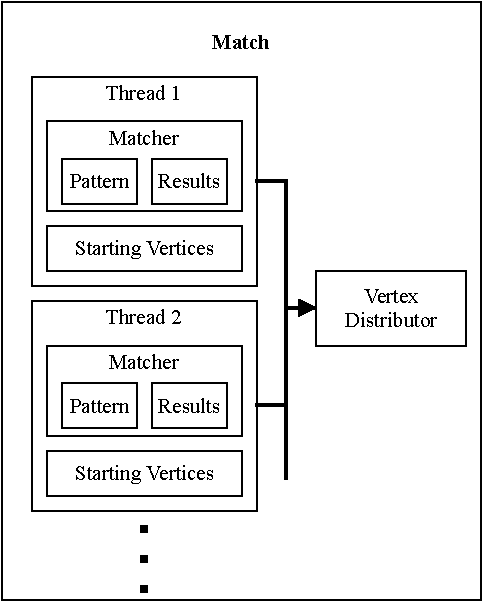
\includegraphics{../img/diaQueryObjectsMatchPar.pdf}\centering
\caption{Diagram paralelizace prohledávání grafu.}
\label{figure.diaQueryObjectsMatchPar}
\end{figure}

\bigskip
\textit{Zbývá nám analyzovat a navrhnout Group by a Order by.
Je nutné si uvědomit potřebu analýzy daných částí.
Analýza nám pomůže pochopit jejich fungování, což nám umožní je lépe porovnat s vylepšenými řešeními. 
Zároveň také tvoří odrazový můstek pro návrh vylepšených řešení.}


\section{Order by}

Order by si klade za cíl setřídit vyhledané výsledky z části Match pomocí zadaných klíčů.
Pořadí klíčů určuje pořadí porovnání.
Výsledky se porovnávají zleva doprava.
To znamená, pokud jsou dva klíče stejné, postoupí se k porovnání s klíčem dalším.
Rovnost dvou výsledků nastává právě tehdy, když mají stejné hodnoty pro všechny klíče. 
Pro klíč se také definuje, jestli má třídění probíhat v rostoucím nebo klesajícím pořadí.
Defaultní pořadí je chápáno jako rostoucí. 
Potřebujeme určit, jakým způsobem budou výsledky hledání setříděny.
Musíme vybrat algoritmus a následně navrhnout způsob efektivního třídění tabulky výsledků.

\subsection{Výběr algoritmů a paralelizace}

Existuje mnoho algoritmů pro třídění.
Chtěli bychom zvolit již prozkoumané a zároveň běžně používané třídící algoritmy.
Mezi náš výběr padli Merge sort nebo Quick sort.
Jsou ideální volba, protože pro ně již existuje paralelní verze.
Při implementaci chceme ideálně použít již existující knihovny nebo implementace. 

\subsection{Quick sort vs Merge sort}

Uvedeme krátké porovnání na základě 3. kapitoly průvodce algoritmů \citep{labyrint}. 
Merge sort má časovou složitost $ \Theta(n\log n) $ i v nejhorším případě, zatímco Quick sort stejné složitosti dociluje pouze v průměrném případě.
V nejhorším případě má $\Theta(n^2)$.
Merge sort potřebuje $\Theta(n)$ pomocné paměti a je to stabilní třídící algoritmus.
Quick sort pouze $\Theta(\log n)$, ale nejedná se stabilní třídění.
K implementaci stabilního Quick sortu je potřeba $\Theta(n)$ pomocné paměti.
Quick sort značně závisí na výběru pivota.
V našem případě bude obtížné ho volit správně, protože nedokážeme říci nic o rozložení tříděných dat.
Z tohoto důvodu bychom volili raději Merge sort.  

\subsection{Třídění pomocí indexů}

Hlavním problémem Order by je třídění tabulky výsledků.
V sekci \ref{anal.tables} jsme definovali formát výsledků a navrhli proxy třídy pro výpočet výrazů.
Setřídit tabulku v našem smyslu znamená setřídit řádky pomocí klíčů zadaných uživatelem.
Pro zjištění shodnosti dvou řádků musíme vypočítat hodnoty jejich klíčů pomocí výrazů a následně je porovnat.
Přesouvání řádků v tabulce, která má více než jeden sloupec, by představovalo značné zpomalení.
Uvedli jsme, že výrazy pro řádky dostanou na vstupu proxy třídu řádků.
Proxy třída se v naší představě získá voláním funkce indexeru na tabulce výsledků.
Daný princip nám umožní vytvořit pole indexů v rozsahu počtu řádek tabulky.
Indexy budou setříděny namísto pravých řádků vybraným algoritmem a při porovnání dojde k získání proxy tříd a výpočtu výrazů.
Přistup nám umožní vyřadit přesouvání řádků, ale zase potřebujeme lineární pamět na pole indexů.
Po dokončení třídění se pole použije jako indexační struktura.

\subsection{Optimalizace porovnání vlastností hodnot} \label{anal.order.opt1}

Třídění obvykle představuje opakované porovnání jednoho prvku s ostatními v řadě za sebou.
Pro pokaždé takové porovnání v řadě počítáme stejnou hodnotu výrazu opakovaně.
Porovnání pomocí \texttt{ID} pouze přistupuje k položce elementu grafu.
Problém nastane, když budeme porovnávat pomocí vlasnosti.
V takovém případě musíme přistoupit k tabulce \texttt{elType} (sekce \ref{anal.grafrep}), zjistit existenci přistupované vlastnosti a následně přistoupit k její hodnotě.
Danou situaci můžeme vyřešit částečně cachování výsledků výrazů.
Budeme si pamatovat poslední porovnané řádky a jejich hodnoty.
Pokud dojde k porovnání řádků pro který byl výraz již vypočítán, tak použijeme zachovanou hodnotu.

\subsection{Optimalizace porovnání stejných elementů}

Dalši možná optimalizace porovnání může nastat v případě, pokud pro použitý graf platí \#Vrcholů $<<$ \#Hran.
Daná vlastnost může mít za následek, že porovnávané řádky budou často obsahovat stejné elementy pro dotazy typu:
\begin{code}
select x.PropOne match (x) -> (y) order by x.PropOne;
\end{code}
V takovém dotazu by hledání mělo vygenerovat několik výsledků se stejným elementem v proměnné x.
Počet takových výsledků zde odpovídá počtu hran vrcholů x.
Abychom předešli opakovanému porovnávání hodnot vlastností stejných elementů, tak než přistoupíme k výpočtu výrazů porovnáme \texttt{ID} přistupovaných elementů.
Tedy využijeme dvou optimalizací.
Budeme si cachovat poslední výsledky výrazů a navíc omezíme porovnání výsledků se stejnými elementy.

\subsection{Optimalizace v paralelním prostření}

Vymysleli jsme optimalizace porovnání.
Doteď jsme však předpokládali, že porovnání probíhá v jednom vlákně.
Druhá optimalizace funguje i v paralelním prostřední, protože se jedná pouze o čtení statických hodnot.
Avšak první optimalizace vytváří problém.
V prvním případě dochází k uchovávání výsledků lokálních pro vlákno a existence sdíleného úložiště by vytvořilo souběh.
Vlákna by se snažila číst a ukládat výsledky ze sdíleného úložiště a docházelo by k nedefinovanému chování.
Problém se dá vyřešit například tak, že každé vlákno bude vlastnit svoje objekty s cachí výsledků.
V průběhu implementace budeme muset najít vhodnou techniku ukládání, aby došlo ke zrychlení třídění.

\section{Group by}

Group by seskupuje výsledky hledání podle uživatelem zadaných klíčů.
Dva výslekdy patří do stejné skupiny právě tehdy, když se shodují ve všech hodnotách klíčů.
Musíme být schopni vypočítat agregační funkce pro skupiny.
K tomu již máme navržené způsoby z sekce Expressions (\ref{anal.expressions}).
Zbývá nám vymyslet způsob ukládání mezivýsledku a algoritmy k vykonání.

\subsection{Módy Group by}

Group by představuje dle našeho pohledu dva módy vykonání.
První mód obsahuje v dotazu část Group by a libovolné množství agregačních funkcí.
Dojde k vytvoření skupin a výpočtu výsledků funkcí pro každou skupinu.
Tento mód budeme označovat \textbf{Group by}.
Druhý mód nemá v dotazu část Group by, ale pouze agregační funkce v ostatních částech.
Zde automaticky dochází k předpokladu, že všechny výsledky patří do stejné skupiny.
Tedy je vytvořena pouze jedna skupina a pro ni se vypočtou hodnoty agregačních funkcí.
Mód nazveme \textbf{Single group Group by}.


\subsection{Úložiště mezivýsledků agregačních funkcí} \label{anal.groupby.uloziste}

V sekci Expressions (\ref{anal.expressions}) jsme navrhli objekt, který obsahuje logiku výpočtu funkce a na vstupu dostává úložiště výsledku.
Očekává se, že pro každou skupinu bude existovat úložiště.
Úložiště musí obsahovat prostor pro výsledky všech počítaných funkcí.
Vymysleli jsme dva způsoby:

\begin{itemize}

\item \textbf{Bucket} - každá skupina bude vlastnit pole objektů. 
Pole bude mít délku rovnou počtu počítaných agregačních funkcí.
Objekty představují úložiště výsledků funkcí.

\item \textbf{List} - výsledky všech skupin jsou uchovávány v dvoudimenzionálním poli, tj. primitivní tabulce.
Sloupeček představuje výsledky jedné agregační funkce.
Jedné skupině pak přináleží řádek.
Každé skipině bude přidělen index řádku.
Nyní pokud budeme chtít výsledky funkcí skupiny, stačí přistoupit skrze přidělený index ke chtěnému výsledku.
\end{itemize}

Následuje ukázka možné implementace dle popisu výše v jazyce C\#:
\begin{code}
Bucket:
\\ Pole výsledků ag. funkcí.
BucketResult[] groupAggFuncResults; 
\\ Objekt úložiště. 
class BucketResult {} 
\\ Objekt definující typ ukládané hodnoty.
class BucketResult<T>: BucketResult { T value; }

List:
ListResults groupsAggFuncResults;
\\ Objekt primitivní tabulky výsledků ag. funkcí.
class ListResults { ListHolder[] holders; }
\\ Objekt jednoho sloupečku tabulky.
class ListHolder {}
\\ Objekt definující typ sloupečku.
class ListHolder<T> : ListHolder { List<T> values }
\end{code}

První způsob je náročnější na paměť oproti druhému způsobu, neboť je zde nutnost vytvářet objekty a pole pro každou skipinu.
Avšak, v druhém způsobu jsme nuceni přistupovat k výsledkům pomocí indirekce.
Výhoda Bucket spočívá v jeho jednoduchém přemisťování (chápeme-li pole jako referenci) a izolaci od ostatních výsledků skupin.
V takovém případě jsme schopni přesouvat výsledky skupiny aniž bychom museli kopírovat jejich hodnoty.
Předpokládáme, že bucket bude výhodnější pro paralelní zpracování díky izolaci od ostatních výsledků, jelikož počet skupin není dopředu znám.
V List budeme muset dynamicky rozšiřovat pole.
Při rozšíření nastane souběh, který budeme muset ošetřit.

\subsection{Logika agregačních funkcí}

Ještě než přistoupíme k výběru zpracování musíme analyzovat logiku agregačních funkcí.
Logika pak ovlivňuje co a jak se bude ukládat v úložišti výsledků.

\begin{itemize}
\item \texttt{Min/Max:} výsledek funkce je minimum/maximum pro skupinu. Při výpočtu dojde k porovnání a následnému uložení hodnoty.
V objektu výsledku musíme znát aktuální minimum/maximum.
Dále, byla-li hodnota již nastavena, protože musíme být schopni rozeznat prázdné úložiště po jeho vytvoření.


\item \texttt{Count/Sum:} výsledek je počet výsledků/suma hodnot výsledků. Při výpočtu musíme přičítat hodnotu k hodnotě v úložišti.
\item \texttt{Avg:} výsledek je aritmetický průměr. Chtěli bychom volit inkrementální metodu. Budeme si ukládat počet výsledků a sumu hodnot výsledků. Pro získání finální hodnoty dojde k vypočtení podílu sumy a počtu výsledků.
\end{itemize}

\subsection{Jednovláknové zpracování}

Po celou dobude budeme pracovat s tabulkou výsledků Match části.
Pro vykonání Group by se nám nabízí několik možností.
První možnost je řádky tabulky setřídit a následně při iteraci výtvářet skupiny a počítat agregační funkce.
Myslíme, že možnost přináší zbytečnou režii za porovnání při třídění, protože pro každé porovnání musíme vypočítat hodnotu výrazu.
Z tohoto důvodu chceme využít strukturu, která bude interně použivát hašovací tabulku (C++ \texttt{std::map<Key, Value>} nebo C\#  \texttt{Dictionary<Key, Value>}).
Záznam v tabulce bude dvojice \texttt{key/value}. 
\texttt{key} je zde index do tabulky výsledků z Match části (nikoliv proxy třída).
Chceme ukládat pouze index abychom ušetřili paměť za pointr na tabulku.
Porovnání vyvolá získání proxy třídy a následné evaluaci hodnot výrazů.
\texttt{value} obsahuje strukturu pro výsledky agregačních funkcí.
Pro Bucket to bude pole objektů a pro List to bude index do tabulky výsledků agregačních funkcí.
Pro výsledek bude vypočítáná haš na základě hodnot klíču a vložena do hašovací tabulky.
Pokud už je obsažen v tabulce, tak se pouze pro získanou \texttt{value} (pole nebo index) aktualizují hodnoty výsledků agregačních funkcí.
V opačném případě bude vložen nový záznam s novou \texttt{value}.
Pro Single group Group by stačí pouze iterovat skrze tabulku a počítat agregační funkce.

\subsection{Optimalizace při výpočtu haš hodnoty}

Minulý přístup nám nabízí jednu optimalizaci k ušetření opakovaného výpočtu hodnoty výrazu klíčů.
Hašovací tabulka při vložení dvojice v prvním kroku vypočte hodnoty klíčů a vypočte jejich haš.
Výsledek se vloží do patřičné přihrádky.
Pokud nastala kolize, tak se prvky musí porovnat.
Při tomto porovnání se opět musí vypočíst hodnoty výrazů vkládané dvojice.
Zde mužeme využít chvíle výpočtu haš hodnoty.
Budeme cachovat hodnoty výrazů a následně je znovu použít při porovnání.
Nicméně, pravděpodobně budeme nutni vytvořit závislost mezi objektem počítajícím haš hodnotu a objektem provádějícím porovnání.
Stejný princip jsme použili při optimalizaci porovnání v sekci \ref{anal.order.opt1}.
Nastávají pro něj také stejné problémy v paralelním prostředí.

\subsection{Paralelní zpracování}

Chceme zvolit několik řešení s rozdílnou úrovní synchronizace, protože nevíme, které bude dosahovat nejrychlejších výsledků.
Navíc nám větší počet řešení umožní lépe porovnat vylepšená řešení.
Pro paralelní zpracování jsme vymysleli tři přístupy: \textbf{Global}, \textbf{Two-step} a \textbf{Local + dvoucestné slévání} (všechny budou schopny pracovat s úložišti Bucket i List).
Každý z nich začíná rozdělením tabulky výsledků Match na ekvivalentní části.
To si můžeme dovolit, neboť máme tabulku obsahující všechny výsledky hledání.
Každé vlákno dostane danou část ke zpracování.
Tím zaručíme rovnoměrnost práce mezi vlákny.
Samotná práce vláken pak zavisí na zvoleném přístupu.
Specifika vykonání jsou popsána v následujících sekcích.

\subsection{Thread-safe agregační funkce}

Ještě než přistoupíme k popisu jednotlivých řešení, je důležité si uvědomit nutnost vytvořit thread-safe verzi objektů implementující logiku agregačních funkcí.
Pro každou funkci bude existovat ekvivalent thread-safe \texttt{Apply} metody.
Samotně pak vyvstává nutnost implementovat thread-safe metody pro slévání výsledků agregačních funkcí.
Problém vyřešeníme přidáním metod do objektů zpravující logiku agregačních funkcí, protože při slévání stále musíme vědět, jak s výsledky správně zacházet.
Pro úpravu logiky agr. funkcí na thread-safe verze volíme tyto varianty:

\begin{itemize}

\item \texttt{Min/Max:} princip Compare and Exchange. V moment porovnání mohlo dojít ke změně hodnoty v úložišti.
Musíme znovu provést porovnání.  

\item \texttt{Sum/Count:} tyto metody implementují pouze přičítání. 
V ideálním případě chceme použít atomické operace přičtění.
 
\item \texttt{Avg:} tuto funkci lze implementovat iterativně. 
Budeme si ukládat součet zpracovaných výsledků a jejich počet.
Finální hodnota pak bude podíl součtu a počtu hodnot.
Tímto můžeme implementovat thread-safe funkci pomocí atomických operací, jako u funkcí \texttt{Sum/Count}.
\end{itemize}

\subsection{Global Group by} \label{anal.groupby.global}

Všechna vlákna budou provádět ekvivalent jednovláknového zpracování pomocí thread-safe paralelní mapy/slovníku (C\# \texttt{ConcurrentDictionary, Java \texttt{ConcurrentHashMap}}).
Skupiny se vytváření globálně.
Všimněme si nutnosti dvojité synchronizace.
Prvě musí dojít k synchronizaci vytváření záznamů v mapě.
Druhý krok synchronizace je nutný při zpracování agregačních funkcí.
Paralelní mapa nám vyřadí souběh při vytváření nových záznamů skupin.
V moment zpracování agregačních funkcí musí dojít k volání thread-safe verzí.
Výhoda této metody je, že nedochází ke slévání, tj. po dokončení práce vlákny jsou výsledky finální.

Bucket reprezentace úložiště má zde značnou výhodu vůči List.
List musí dynamicky rozšiřovat tabulku svých výsledků.
Místo abychom použili dvojí synchronizace jako u Bucket, tak zde bude nutné představit ještě třetí krok synchronizace.
Při přístupu do tabulky je nutné kontrolovat, jestli se nemusí rozšířit.
V ten moment se musí zabránit přístupu ostatních vláken a teprve pak rozšířit tabulku.
To se dá implementovat například semaforem omezující pohyb vláken v kritické sekci.
Vlákno v moment nutnosti rozšíření zablokuje vstup přes semafor.
Vlákno se na přístup pokusí projít skrze semafor, pokud je mu vstup zabráněn tak dochází k rozšiřování tabulky.
V opačném případě aktualizuje výslednou hodnotu agregační funkce.
Postup s List může být však značně pomalý a proto budeme uvažovat, jestli přístup raději implementovat pouze pro Bucket.
Global Group by je znázorněn na obrázku \ref{figure.diaGlobalGr}.

\subsection{Two-step Group by} \label{anal.groupby.twostep}

Tento přístup probíhá ve dvou krocích.
Lokální část nasledovaná globální částí. 
V lokální části pro každé vlákno běží kompletně identický ekvivalent jednovláknového zpracování.
Globální část nastane v moment dokončení této práce.
Místo aby vlákno ukončilo běh, tak rovnou provede slévání svých výsledků do thread-safe paralelní mapy.
To znamená, že vlákno nečeká na dokončení práce ostatních vláken, ale rovnou slévá své výsledky do paralelní mapy.
Tento přístup kombinuje jednovláknové řešení společně s přístupem Global.
Mínus je, že zde musí docházet ke slévání, ale v prvním kroku se využívají metody, které nemusí řešit synchoronizaci. 
Problematická část je zde slévání výsledků s List úložištěm výsledků agregačních funkcí.
První fáze nepředstavuje problém. 
Druhá představuje problém jako u Global řešení, tedy platí vše, co jsme pro něj zmínili.
Můžeme zkusit implementovat stejné řešení jako u Global pomocí semaforu.
Two-step Group by je znázorněn na obrázku \ref{figure.diaTwoGr}.

\subsection{Local + dvoucestné slévání Group by} \label{anal.groupby.local}

Přístup nepoužívá thread-safe metody ani paralelní mapu.
Opět rozdělíme přístup na dvě části.
V prvník kroku pro každé vlákno běží identický ekvivalent jednovláknového zpracování.
Po dokončení se spustí dvoucestný slévání na výsledky vláken.
Slévání bude připomínat binární strom.
Listy představují lokální seskupování vláken.
Vnitřní vrcholy stromu představují slévání výsledků.
Finální výsledek je vytvořen v kořeni.
U slévání využijeme paralelního zpracování.
Při slévání vždy jedno vlákno ukončí běh, druhé z dvojice provede slévání a postoupí ke kořeni. 
Hlavní výhody byly už zmíněny.
Používají se metody bez synchronizace.
Nevýhoda řešení je, že vlákna musejí čekat při slévání na dokončení práce druhého vlákna a teprve až pak může dojít ke slévání.
Přístup je znázorněn na obrázku \ref{figure.diaLocalGr}.

\subsection{Paralelizace Single group Group by}

K paralelizaci Single group Group by se nám poskytuje využít jíž zmíněných principů.
Konkrétně zde mají využítí všechny tři.
Slévání všech výsledků do jednoho úložiště výsledků agregačních funkcí z principu Global.
Problémem tohoto přístupu je synchronizace mnoha vláken na jednom místě.
Ideálnější je využít lokálního zpracování zbylých dvou metod.
Opět řešení rozdělíme na dva kroky. 
V prvním kroku každé vlákno provádí ekvivalent jednovláknového zpracování bez vytváření skupin, tj. počítá pouze agregační funkce pro jednu skupinu.
Výsledky se následně musí slévat.
K rozhodnutí, které řešení finálně použít použijeme fakt, že počet výsledků k slévání je roven počtu vláken.
V takovém případě nebudeme implementovat paralelní slévání, ale pouze jedno vybrané vlákno provede sjednocení všech výsledků.


\begin{figure}[!htp]
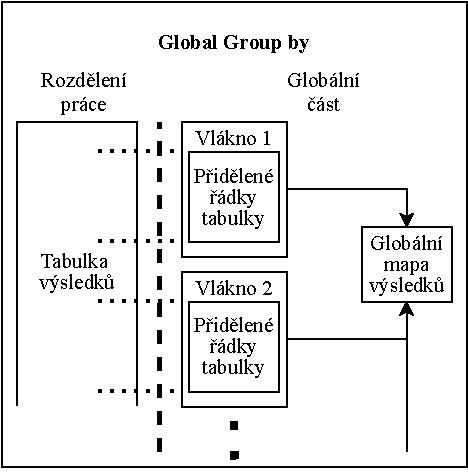
\includegraphics{../img/diaGlobalGr.pdf}\centering
\caption{Diagram paralelizace Global Group by.}
\label{figure.diaGlobalGr}
\end{figure}

\begin{figure}[!htp]
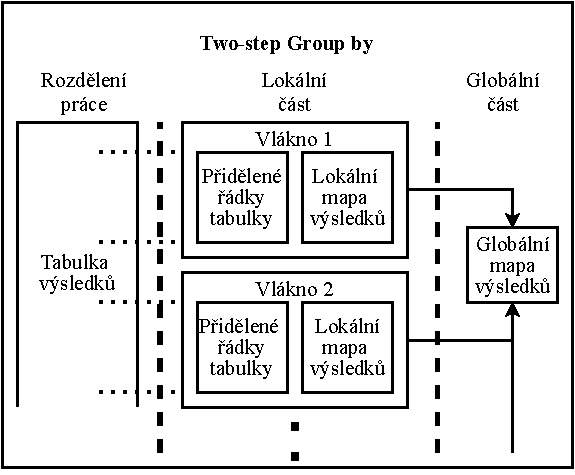
\includegraphics{../img/diaTwoGr.pdf}\centering
\caption{Diagram paralelizace Two-step Group by.}
\label{figure.diaTwoGr}
\end{figure}

\clearpage

\begin{figure}[!htp]
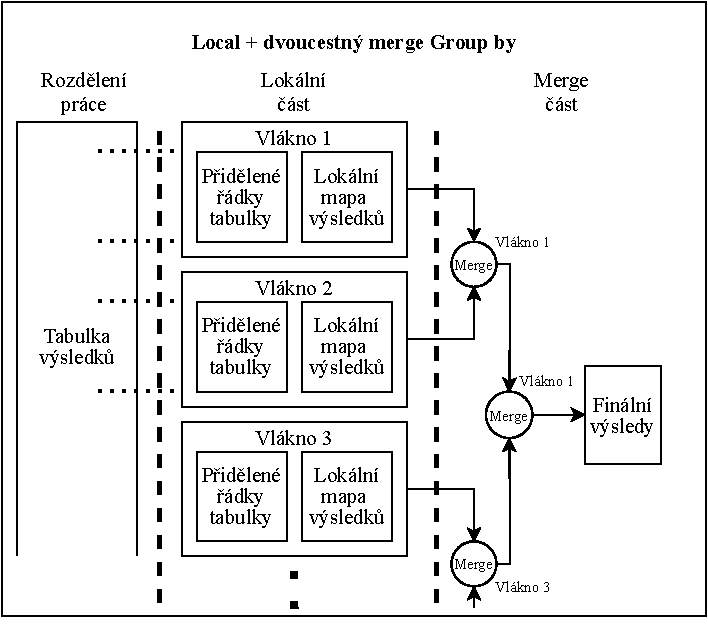
\includegraphics{../img/diaLocalGr.pdf}\centering
\caption{Diagram paralelizace Local + dvoucestné slévání Group by pro 4 vlákna.}
\label{figure.diaLocalGr}
\end{figure}

\bigskip
\textit{Analyzovali jsme a navrhli řešení vykonání částí Match, Group by a Order by.
Tímto jsme dokončili analýzu a návrh dotazovacího enginu.
Daná analýza a návrh nám poskytnou odrazový můstek při analýze úprav pro vykonání částí Group by a Order by v průběhu hledání.
}
%%%%%%%%%%%%%%%%%%%%%%%%%%%%%%%%%%%%%%%%%%%%%%%%%%%%%%%%%%%%%%

\section{Úprava enginu} \label{anal.improvement}

Cílem úprav je poskytnout enginu schopnost provádět části Group by a Order by v průběhu prohledávání grafu části Match.
Obecně to znamená, že v moment nalezení jednoho výsledku jej musíme okamžitě zpracovat.
Pro Order by to znamená výsledek správně zatřídit do již setříděné posloupnosti výsledků.
Pro Group by to znamená výsledek přidat do správné skupiny nebo pro něj skupinu vytvořit, navíc musíme pro něj zpracovat agregační funkce. 
Čili, výsledky v průběhu hledání Match části nebudeme ukládat do tabulky, která se po nalezení všech výsledků předá k dalšímu zpracování.
Namísto toho navrhneme postup, kterým docílíme zpracování výsledků v moment jeho nalezení.
Postupy ověříme vůči stávajícím řešením v kapitole Experiment \ref{expr} z hlediska doby vykonání.
V ideálním případě docílíme zrychlení nebo pouze vyrovnání vůči řešením vykonávající Order by a Group by po dokončení hledání.
Z hlediska implementace to také znamená naprogramovat vylepšení tak, abychom byli schopni jednoduše přepínat mezi způsobem vykonání dotazu.
Řešení tedy musí fungovat nezávisle na sobě. 
V prvním kroku úprav musíme získat obecný pohled na pozměněný způsob vykonání dotazu.
Následně v dalších krocích budeme navrhovat části dotazu konkrétněji.

\subsection{Pohled na pozměněný způsob vykonání dotazu}

V následujicích sekcích popíše náš obecný pohled na zpracování dotazu.
Budeme vycházet z sekce \ref{anal.vykonanidotazu}.
V dané sekci jsme si definovali prioritu částí dotazu.
Priorita určovala pořadí vykonání:
\begin{code}
Match > Where > Group by > Having > Order by > Select
\end{code}
Match se provedl jako první.
Následně se nalezené výsledky předávali dalším částem ve směru klesající priority.
Nejvyšší priorita se nachází nalevo a nejnižší napravo.
Pro naše potřeby úprav budeme nyní uvažovat pouze části Match, Group by, Order by a Select.
Opět budeme o částech uvažovat jako o separátních objektech.
Potřebujeme, aby Match část v moment nalezení výsledku jej předala k zatřídění části Order by nebo k seskupení části Group by.
Po zatřídění/seskupení se opět pokračuje v prohledávání grafu, dokud se nenajde další výsledek a ten se zase předá k dalšímu zpracování.
Můžeme si všimnout značné podobnosti s předchozím návrhem. 
Jediný rozdíl je ten, že místo předání všech výsledku najednou další části se předá výsledek pouze jeden.
Na Match část se můžeme dívat jako na kontinuální generátor výsledků. 
V momentě nalezení se výsledek pošle dálším částem.
Zbylé části pak pouze čekají na moment příchozího výsledku.
Finální výsledky budou uchovány v objektech částí Group by nebo Order by. 

Otázkou je, co je zde předávaný výsledek.
Budeme předpokládat, že předávaný výsledek ke zpracování je pole promenných definové v sekci hledaného vzoru \ref{anal.match.res}.
To znamená, že předané pole se nesmí měnit, protože pole náleží struktuře vzoru.
Tedy pokud s ním chceme pracovat přímo, musíme vytvořit kopii.
\textbf{Když budeme hovořit o výsledku hledání, tak máme na mysli dané pole proměnných.}

\subsection{Order/Group by část jako bariéra}

Problematická sekce návrhu je část Select.
Pokud dotaz neobsahuje další části, pak v době nalezení výsledku jej stačí pouze vypsat.
Nicméně, pokud je v dotazu obsažen Group by nebo Order by, pak se výsledky mohou vypsat až po dokončení třídění nebo seskupování.
Tedy dané dvě části nám tvoří bariéru, skrze kterou nemůže posílat výsledky dále.
Jelikož máme navrhnout pouze vykonání částí Order by a Group by, tak budeme uvažovat pro Match a Select stejný návrh, jako v minulých sekcích.
Tedy dotaz bude tvořen původní částí Select propojenou s části Match.
Část Match pak propojíme s částmi Order/Group by a upravíme tak, aby jim byla schopna předávat jeden výsledek v moment jeho nalezení.  

\subsection{Změna objektů reprezentující části Order/Group by}

Řekli jsme, že budeme opět považovat části dotazu za separátní objekty.
Vytvoříme nové objekty částí Group/Order by reprezentující nový způsob zpracování.
Abychom byli schopni pracovat souběžně i s původními objekty, tak potřebujeme upravit objekt Match, protože musí chápat nový způsob zpracování. 
Reprezentanty částí Order by a Group by budou nyní nové objekty (obrázek \ref{figure.diaStreamedResultProcessor}).
Budou si implementovat logiku zpracování jednoho výsledku v metodě \texttt{ProcessResult}.
Objekt zároveň obsahuje finální výsledky dotazu, proto potřebujeme metodu \texttt{RetrieveResults} na jejich získání.

Dotaz bude reprezentován opět řetězcem jako před úpravou zpracování.
Select a Match budou tvořit propojení objetků na základě UML diagramů \ref{figure.diaQueryObjects} a \ref{figure.diaQueryObjectsCon}.
Propojení objektu Match s novými objekty Group by a Order by navrhneme v dalších částech.

\begin{figure}[!htp]
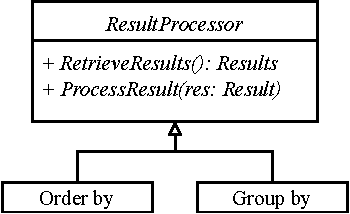
\includegraphics{../img/diaStreamedResultProcessor.pdf}\centering
\caption{UML class diagram nových objektů reprezentující části Group by a Order by.}
\label{figure.diaStreamedResultProcessor}
\end{figure}

\subsection{Propojení nových objektů s objektem Match}

Vytvořili jsme nové objekty a nyní je musíme propojit s objektem Match.
Objekty budou propojeny na dvou úrovních.
První úroveň bude přímé spojení nových objektů s objektem Match a druhá úroveň bude propojení vyhledávání a zpracování výsledku.

\subsubsection{Přímé spojení objektů}

Popíšeme realizaci první úrovně propojení, tj. objekt Match drží odkaz na objekt Group/Order by.
Abychom realizovali tuto úroveň, tak musíme upravit objekt Match.
Objekt Match rozšíříme o chápání logiky nových objektů (obrázek \ref{figure.diaStreamedQueryObjects}).
Stávající objekt Match jsme v naši představě pouze rozšířili a nevytvářeli kompletně nový objekt, protože propojení s Select objektem je realizováno stále původním způsobem.
Finální propojení objektů je pak znázorněno na obrázku \ref{figure.diaStreamedQueryObjectsCon}.

\begin{figure}[!htp]
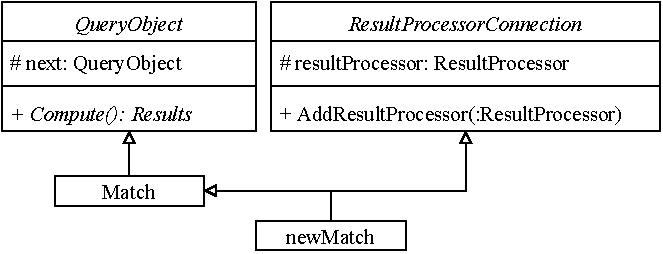
\includegraphics{../img/diaStreamedQueryObjects.pdf}\centering
\caption{UML class diagram rozšířeného objektu Match. Objekt nyní drží přímý odkaz na \texttt{ResultProcessor} a zároveň implementuje původní logiku objektu.}
\label{figure.diaStreamedQueryObjects}
\end{figure}

\begin{figure}[!htp]
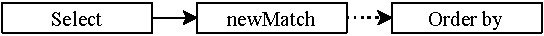
\includegraphics{../img/diaStreamedQueryObjectsCon.pdf}\centering
\caption{Diagram objektů upraveného vykonání představující části dotazu select x match (x) order by x. Plná šipka znázorňuje původní propojení a tečkovaná šipka představuje nové nové propojení.}
\label{figure.diaStreamedQueryObjectsCon}
\end{figure}


\subsubsection{Propojení vyhledávání a zpracování výsledku}

Musíme ještě navrhnout způsob předávání výsledků částem Order/Group by v průběhu hledání.
Způsob musí být použitelný pro paralelní zpracování, proto budeme rovnou přemýšlet nad paralelním řešením.
V naši představě budeme vycházet přímo z původního návrhu z sekce \ref{anal.match}.
Definovali jsme si, že každé vlákno vlastní lokálně strukturu vzoru \texttt{Pattern}, objekt vyhledávání \texttt{Matcher} a tabulku výsledků.
Finální výsledky ukládá do tabulky a po dokončení hledání dojde k slévání tabulek.
Zde upravíme část, kdy dochází k ukládání výsledků do tabulky.
Vlákno bude držet odkaz na objekt Group/Order by a v moment nalezení výsledek předá pomocí volání metody \texttt{ProcessResult}.
Metoda výsledek zpracuje a po návratu z metody se pokračuje ve vyhledávání.
To se opakuje dokud prohledávání neskončí.

Zpracování dotazu bude finálně vypadat následovně.
Na řetězci objektů se zavolá metoda \texttt{Compute}.
První objekt v řetězci je Select.
Select rekurzivně zavolá metodu na části Match a ta spustí vyhledávání.
Část Match prohledává graf a výsledky předává části Order/Group by pomocí metody \texttt{ProcessResult}.
Po dokončení prohledávání volaná metoda \texttt{Compute} na objektu Match získá zpracované výsledky z další části pomocí volání metody \texttt{RetrieveResults}.
Výsledky se tímto předají části Select k vypsání uživateli. 

\subsection{Alternativní řešení}

Při výberu tohoto řešení jsme uvažovali ještě nad možností, ve které by vlákna vyhledávání pouze předávali pouze do fronty.
Další část by pouze zpracovávala výsledky z fronty.
Myslíme, že tohle řešení by bylo neefektivní v našem případě, protože by muselo docházet k synchronizaci fronty, tj. problém producent a spotřebitel.
V našem řešení jsme synchronizaci při předávání výsledků zcela vynechali.

\bigskip
\textit{
Vytvořili jsme nové objekty částí Order by a Group by.
Propojili jsme původní objekty s novými a nyní přejdeme k analýze a návrhu samotných způsobů vykonání Order by a Group by.}

\subsection{Obecný model vykonání Order/Group by}

Pokud bychom realizovali pouze jednovláknové vykonávání, tak bychom z předchozích sekcí měli již kompletní návrh.
Pomocí volání metody \texttt{ProcessResult} dojde k předání výsledků a následnému zpracování.
Problematická část je paralelizace vykonání.
Musíme být schopni zpracovávat výsledky z množství vláken v jeden okamžik.
Je nutné aby docházelo k synchronizaci.
Ještě než přistoupíme k konkrétním návrhům algoritmům zpracování.
Navrhneme obecný model paralelního zpracování.
Vymysleli jsme dva modely, které využijeme při našem zpracování výsledků v průběhu hledání.
Modely \textbf{Streamed} a \textbf{Half-Streamed}.
Modely jsme vybrali na základě množství využívané synchronizace a množství slévání výsledků.
Chceme vytvořit větší množství řešení, abychom mohli lépe porovnat výsledky v kapitole Experiment \ref{expr}.

\subsubsection{Návrh Streamed}

Prvním modelem vykonání je model \textbf{Streamed}.
Myšlenkou tohoto návrhu je příchozí výsledky zpracovat globálně.
Vycházíme z Global zpracování Group by z sekce \ref{anal.groupby.global}.
Vytvoříme strukturu, která nám poskytne metody se synchronizací.
Všechna vlákna v moment nalezení výsledku volají metodu \texttt{ProcessResult}, uvnitř které dojde k volání synchronních metod na struktuře.
Výhoda tohoto přístupuje je odstranění nutnosti slévání výsledků vláken.
Nevýhoda je, že zde dochází k volání metod se synchronizací.
Tyto metody můžou způsobit značné zpomalení při vykonávání kvůli režii za danou synchronizaci.

\subsubsection{Návrh Half-Streamed}

Druhým modelem vykonání je model \textbf{Half-Streamed}.
Myšlenkou tohoto návrhu je příchozí výsledky zpracovat ve dvou krocích.
V prvním kroku každé vlákno výsledky zpracovává lokálně.
Po dokončení vyhledávání dojde ke slévání výsledků vláken.
Vycházíme z řešení \textbf{Two-step} a \textbf{Local + dvoucestné slévání} Group by z sekcí \ref{anal.groupby.twostep} a \label{anal.groupby.local}.
Výhodou tohoto přístupu je využití zpracování bez nutnosti synchronizace vláken v prvním kroku.
Nevýhoda je, že zde dochází ke slévání výsledků po dokončení zpracování.

Nyní jsme si uvědomili problém vznikající voláním metody \texttt{ProcessResult}.
Logika zpracování náleží objektům Group by a Order by.
Objekty zde musí vědět, že dochází nejdříve k lokálnímu zpracování.
Proto jsme rozšířili metodu o další formální parametr \texttt{MatcherID}.
Parametr symbolizuje \texttt{ID} vyhledávače (\texttt{Matcher}) vlákna.
Objekty Group by a Order by pak budou vlastnit lokální výsledky vláken, které budou přístupné skrze \texttt{MatcherID}.
Při volání metody \texttt{ProcessResult} dojde ke zpracování výsledku nad danými lokálními výsledky.
Po dokončení dojde ke slévání výsledků vláken.


\section{Úprava Single group Group by}

Single group Group by je mód, ve kterém uživatel zadal v dotazu výpočet agregačních funkcí, ale nezadal část Group by.
V tomto případě všechny výsledky hledání náleží pouze do jedné skupiny, pro kterou se počítají dané agregační funkce.
V původním řešení se mód vykonával následovně.
Prohledávání grafu nalezlo všechny výsledky a uložilo je do tabulky výsledků.
Po dokončení hledání dochází ke zpracování výsledků.
V jednovláknovém vykonání dojde k iteraci všech výsledků a průběžné aktualizaci hodnot agregačních funkcí.
V paralelním zpracování dojde k rovnoměrnému rozdělení výsledků mezi vlákny a vlákna počítají agregační funkce lokálně.
Po dokončení jedno vybrané vlákno provede slévání výsledků agregačních funkcí.

Stačí nám tedy navrhnout způsob vykonání pro naše dva módy \textbf{Streamed} a \textbf{Half-Streamed}.
Budeme uvažovat pouze paralelní řešení, protože jednovláknové bude pouze určitý případ paralelního.
Obecně si můžeme si všimnout, že výsledky se nemusí ukládat do tabulky.
Po nalezení výsledku dojde k aktualizaci hodnot agregačních funkcí a výsledek není dále potřeba, proto jej můžeme zahodit.
Ušetříme tedy spoustu paměti za tabulku výsledků.
Samotný výpočet hodnot funkcí a úložiště hodnot budou totožné s původním řešením.

\subsubsection{Half-Streamed}

V tomto módu každé vlákno počítá hodnoty agregačních funkcí lokálně.
Po nalezení výsledku dojde k aktualizování lokálních hodnot agregačních funkcí.
V moment dokončení hledání všech vláken dojde ke slévání výsledků vláken.
Samotné slévání můžeme implementovat totožným způsobem jako původní řešení.
To znamená, že jedno vybrané vlákno bude slévat všechny lokální výsledky vláken, když dojde k ukončení hledání všemi vlákny.
Výhoda tohoto řešení je vyřazení nutnosti používat thread-safe logiku agregačních funkcí.

\subsubsection{Streamed}

V tomto módu existuje pouze jedno sdílené úložiště hodnot agregačních funkcí.
Vlákna v moment nalezení výsledku aplikují thread-safe agregační funkce.
Výhoda tohoto řešení je, že zde nedochází ke slévání výsledků.
Problém zde může nastat ve chvíli, kdy existuje velké množství přistupujících vláken.
Všechna vlákna se synchronizují v jednom místě.
Tato synchronizace může mít za následek značné zpomalení zpracovávání

\smallskip
Všimněme si také, že v jednovláknovém zpracování jsou módy totožné.
V obou případech se nemusí použít thread-safe logika agregačních funkcí a existuje pouze jedno úložiště hodnot.
Módy se tedy liší jen způsobem paralelního zpracování.


\section{Úprava Group by}

Group by má za úkol seskupit výsledky dle zadaných klíčů a vypočíst hodnoty zadaných agregačních funkcí.
Při úpravě budeme využívat původní úložiště (List a Bucket) a logiku agregačních funkcí.
Opět budeme při zpracování chtít použít hašovací tabulku jako původní řešení.
Přejdeme rovnou k návrhu zpracování módů \textbf{Streamed} a \textbf{Half-Streamed}.
Budeme uvažovat paralelní řešení, protože jednovláknové zpracování je určitý případ paralelního.

\subsection{Half-Streamed}

V tomto módě chceme pouze upravit původní řešení Two-step z sekce \ref{anal.groupby.twostep}.
Má totiž stejný průběh vykonání jako samotný model \textbf{Half-Streamed}.
Oba pracují s myšlenkou práce ve dvou krocích.
V prvním kroku dochází k lokálnímu vytváření skupin a po dokončení hledání dojde ke slévání výsledků vláken.
Vlákno po dokončení hledání nečeká na dokončení práce ostatních vláken, ale rovnou výsledky slévá do sdíleného úložiště.
Zmiňovali jsme, že se jedná o paralelní mapu/slovník (C\# \texttt{ConcurrentDictionary}, Java \texttt{ConcurrentHashMap}).
Nepoužijeme zde řešení Local + dvoucestné slévání, protože samotné slévání vytváří nutnost vláken čekat na dokončení práce jiného vlákna.
Pomocí řešení Two-step se problému kompletně vyhneme.

\subsubsection{Ukládaní pouze reprezentantů skupin}

K upravení původního řešení musíme pouze vyřešit problém chybějící tabulky výsledků, protože v moment nalezení výsledku je výsledek předán části Group by a není tak uložen do tabulky.
Mohli bychom výsledky opět ukládat do tabulky.
V moment nalezení je výsledek překopírován do tabulky na nový řádek a proxy třídu řádku využijeme k jeho zpracování.
Daný způsob nám příjde neefektivní, protože cílem Group by je vytvořit skupiny. 
K vytvoření skupin nám stačí znát pouze reprezentant skupiny, tj. klíč v hašovací tabulce (proxy třída řádku v tabulce výsledků hledání).
Nepotřebujeme znát všechny výsledky hledání, tedy nemusíme všechny výsledky kopírovat do tabulky.
Abychom mohli pouze minimálně upravit vykonávání řešení Two-step, tak upravíme původní tabulku výsledků na základě tohoto poznatku.
Tabulka bude nyní kromě samotných hodnot obsahovat položku držící odkaz na výsledek hledání.
V moment nalezení výsledku se odkaz aktualizuje na daný výsledek a tabulka bude tento akt chápat jako přidání nového imaginárního řádku.
Při přístupu k novému řádku se vytvoří obvyklá proxy třída řádku.
Následný přístup k hodnotám řádku skrze proxy třídu vyvolá čtení hodnot z odkazu a nikoliv hodnot z tabulky.
Proxy třída se použije ke zpracování výsledku hledání.
Pokud byla proxy třída použita k vytvoření nové skupiny, tj. je vytvořen nový záznam v hašovací tabulce, tak je celý výsledek držený v odkazu překopírovan do tabulky.
Tímto si zachováme pouze reprezentanty skupin a díky používání odkazu nemusíme každý výsledek hledání kopírovat do tabulky.

\smallskip
Zbytek zpracování bude totožný s původním řešením Two-step.
Úložiště hodnot agregačních funkcí bude implementováno rovněž totožně.
Platí pro něj obdobné problémy, které jsme již zmínili v sekci popisu daného zpracování \ref{anal.groupby.twostep}. 


\subsection{Streamed}

Při tomto řešení budeme vycházet z přístupu Global Group by z sekce \ref{anal.groupby.global}, protože zpracovává výsledky stejným způsobem jako model \textbf{Streamed}.
Existuje zde jedna sdílená thread-safe struktura, ke které přistupují všechna vlákna.
Jedná se opět o paralelní mapu/slovník.
Předpokládejme nyní, že budeme chtít stále používat tabulky výsledků a stejná úložiště agregačních funkcí.

\subsubsection{Problém synchronizace tabulky výsledků}

Vyvstává zde opět problém neexistující tabulky výsledků.
Opět chceme ukládat pouze reprezentanty skupin.
Nicméně, problém je zde komplikovanější, protože v minulé sekci jsme tabulky vytvářeli lokálně.
Tedy v moment slévání byly tabulky již finální. 
Aplikujeme-li nyní přístup lokálních tabulek, tak vyvstává další problém.
Vlákna v průběhu vyvolávají porovnaní klíčů v hašovací tabulce.
Klíč je zde proxy třída řádku v tabulce.
Skrze proxy třídu vlákno přistoupí k elementům na řádku tabulky.
V tuto chvíli však můžou přistupovat k hodnotám v tabulce i jiná vlákna a zároveň může docházet k rozšíření tabulky.
Pokud by docházelo k rozšiřování tabulky, tak zde dojde k souběhu a přistoupení k nevalidní tabulce.
Problém se dá řešit například použitím zámku.
Při každém přistupu k tabulce by došlo k získání zámku, následnému vyvolání porovnání nebo rozšíření a nakonec uvólnění zámku.
Řešení však přínáší nutnou režii za synchronizaci tabulky, proto jsme se od řešení pomocí tabulky rozhodli kompletně upustit.

\subsubsection{Nový přístup ukládání výsledků}

Úložiště hodnot agregačních funkcí budou pořád totožná.
Místo ukládaní výsledků do tabulky vypočteme konkrétní hodnoty klíčů Group by.
Hodnoty uložíme do pole, které následně použijeme jako klíč paralelní mapy.  
Samotné pole elementů použijeme pouze k výpočtu hodnot klíčů a k aktualizaci hodnot agregačních funkcí.
Následně jej zahodíme.
Paralelní mapa bude ve výsledku obsahovat pole hodnot klíčů a pole hodnot agregačních funkcí.
Samotné hodnoty klíčů jsou v moment vytvoření statické, tedy nikdy nedojde ke změně hodnot klíče.
Vlákna mohou jednoduše vyvolat porovnání klíčů bez nutnosti synchronizace.

Ačkoliv se může zdát, že vytvářením mnoha malých polí povede k značné paměťové zátěži.
Musíme si uvědomit, že budeme uchovávat pouze ta pole, která byla vložena do paralelní mapy.
Obecně předpokládáme, že počet finálních skupin je mnohonásobně menší než počet výsledků hledání.
Tedy bude zde existovat pouze malá množina polí.
Otázka může být, proč jsme nezvolili daný postup i u ostatních řešení.
V původním řešení jsme drželi všechny výsledky v paměti a vytváření dalších polí spolu s překopírovávání výsledků by ještě víc vytížil paměťovou spotřebu.
V \textbf{Half-Streamed} řešení jsme způsob nepoužili, protože výsledky vláken se vytvářeli lokálně.
Kdyby každé vlákno našlo kompletně stejné skupiny, pak by existovala totožná pole pro všechna vlákna.

Další otázka je proč jsme se rozhodli uchovávat hodnoty výrazů a ne elementy grafu.
Hlavní příčina ukládání elementů jsme popsali v sekci návrhu tabulky výsledků hledání \ref{anal.tables}.
Tento problém zde odpadá, protože ukládáme malé množství výsledků.
Navíc, v ostatních částech dotazu se mohou vyskytnout pouze výrazy klíčů Group by a agregační funkce.
Tedy v moment výpočtu daných výrazů a agregačních funkcí jsme získali všechny možné hodnoty, ke kterým se může přístoupit v jiných částech dotazu. 

\subsubsection{Sloučení pole klíčů a pole úložiště agregačních funkcí}

Nabízí se zde malá optimalizace za předpokladu, že budeme používat Bucket úložiště agregačních funkcí.
Bucket úložiště je pole hodnot.
Můžeme zde propojit pole hodnot klíčů a pole hodnot úložiště, protože oba pole pouze obsahují konkrétní hodnoty a logika zpracování agrgačních funkcí je obsažena v objektu mimo úložiště.
Finálně bude existovat pouze jedno pole, ve kterém prvních $n$ hodnot představuje hodnoty klíčů a zbytek hodnot je považován za výsledky agregačních funkcí.
Tímto dokážeme zmenšit počet vytvářených polí.
Protože vycházíme z principu Global Group by \ref{anal.groupby.global}, tak je zde problémem úložiště List.
Rozhodli jsme dané řešení neimplementovat.

\bigskip
\textit{Analyzovali jsme a navrhli úpravu řešení Group by a Single group Group by. 
Nyní přejdeme k úpravě Order by.}

\section{Úprava Order by}

Cílem Order by je setřídit výsledky hledání.
V původním řešení jsme měli značnou výhodu, protože v moment začátku třídění jsme vlastnili všechny výsledky hledání (tj. kompletní tabulka výsledků).
Místo třídění samotných řádků tabulky jsme třídili pole indexů.
Na pole indexů pak stačilo aplikovat zákládní třídíci algoritmus.
Nyní nevlastníme všechny výsledky.
Výsledky jsou generovány a zpracovávány postupně.
V následujících sekcích navrhneme způsob zpracování Order by v průběhu hledání.

\subsection{Obecný princip zpracování}

V naši představě zpracování budeme udržovat setříděnou posloupnost výsledků hledání.
Při nalezení výsledku výsledek zatřídíme do již setříděné posloupnosti.
Obecně jsme se rozhodli použít následující princip.
Bude existovat totožná tabulka výsledků hledání jako v původním řešení společně s indexační strukturou tabulky, protože nechceme přesouvat řádky tabulky.
Indexační struktura bude opět obsahovat indexy řádků v tabulce.
Výsledek Order by pak bude tabulka výsledku s indexační strukturou.

Výsledek hledání v moment nalezejí je vložen na nový řádek tabulky výsledků.
Následně je index nového řádku tabulky zatříděn do indexační struktury.
Z tohoto principu budeme vycházet v našem návrhu.
Nejdříve budeme analyzovat způsob jednovlákonvého zpracování a následně jednotlivé módy paralelního zpracování.

\subsection{Jednovláknové zpracování} \label{anal.ordeby.single}

Určili jsme, že tabulka výsledků je totožná s původní.
Výsledek je vložen na nový řádek tabulky a index je zatříděn do indexační struktury.
Potřebujeme jen navrhnout způsob zatřídění indexu do indexační struktury.
Uvažovali jsme nad dvěma základními přístupy.
První kombinuje pole indexů s binárním vyhledáváním.
Druhý přistup využívá vyhledávací stromy.
Přistupy popíšeme a následně provedeme malý experiment.

\subsubsection{Pole indexů + binární vyhledávání}

Myšlenka přístupu je udržovat setříděné pole indexů. 
V moment nalezení výsledku je využito binární vyhledávání \citep[str. 26]{labyrint} k nalezení vhodného místa vložení do pole.
Prvek je vložen do pole.
Pokud se na místě nacházel již nějaký prvek, prvek je posunut doprava.
Pokud v poli není dostatek místa, tak je rozšířeno.
Jedná se vlastně o algoritmus Insert sort (třídění vkládáním).
Jediným rozdílem je, že k nalezení místa vložení se používá binární vyhledávání.

Problém zde představuje posouvání prvků v poli.
Předpokládáme-li, že prvky posouváme napravo, tak v nejhorším případě vložením na začátek pole posuneme všechny prvky.
V naši představě bychom chtěli problém řešit rozmístěním mezer mezi prvky v poli.
Mezerou zde rozumíme prázdný záznam, tj. neobsahuje žádný index tabulky výsledků.
Mezi každými dvěma sousedními prvky by existoval stejný počet prázných záznamů.
Vložení by bylo opět realizováno binárním vyhledáváním.
V sitauci posouvání prvků nyní stačí posouvat prvky do první mezery.
Řešení však naskýtá spoustu otázek.
Například neznáme ideální počet mezer mezi prvky a nevíme jak optimálně navrhnout binární vyhledávání na takovém poli.
Navíc, zvyšováním počtu mezer se pole značně zvětšuje, tj. roste paměťová složitost.

\subsubsection{Vyhledávací stromy}

Druhý přístup využívá vyhledávací stromy \citep[str. 177]{labyrint}.
Chtěli bychom využít základní druhy vyhledávacích stromů jako binární vyhledávací stromy nebo $(a, b)$-stromy.
Výhoda $(a, b)$-stromů je ta, že každý vrchol stromu obsahuje až $b-1$ klíčů, zatímco binární vyhledávací stromy drží pouze jeden klíč ve vrcholu.
Pokud bychom implementovali řešení s vyhledávacími stromy, tak budeme ideálně chtít využít již stávajících knihoven.

\subsubsection{Experiment pole vůči vyhledávácím stromům}

K porovnání dvou přístupů jsme se rozhodli provést jednoduchý experiment.
Cílem testu je otestovat rychlost vkládání prvků do vybraných datových struktur.
Test bude částečně simulovat reálnou činnost zatřiďování prvků do struktury.
Experiment jsme naprogramovali v jazyce C\#.
Kód je součástí příloh \ref{prilohy.benchtreevsarray}.
Kód jsme přeložili pro platformu Windows 10 x64 cílící na .Net Framework 4.8.
Samotný hardware testovacího stroje je rozepsán v sekci metodiky \ref{expr.hw}.
K otestování jsme vybrali dvě nativní struktury C\#:

\begin{enumerate}
\item \texttt{List}: reprezentuje případ zatřiďování do pole binárním vyhledáváním.
\item \texttt{SortedSet}: reprezentuje případ binárního vyhledávacího stromu.
\end{enumerate}
Struktury jsme zaplnili $n$ náhodně generovanými prvky.
Prvky byly generovány nativní třídou \texttt{Random} s inicializační hodnotou 100100 v rozsahu hodnot $[10$ $000; Int32.MaxInt - 10$ $000]$.
Struktury byly setříděny.
Následně jsme do struktur vkládali $m$ náhodně generovaných prvků (totožnou třídou \texttt{Random}) z dvou různých rozsahů:

\begin{enumerate}
\item Rozsah $[0; 10$ $000]$ a je označen $front$. 
Umožní nám vkládat prvky na začátek setříděné posloupnosti. 
Sledujeme nejhorší případ pro pole, kdy dochází k posouvání všech prvků doprava.
\item Rozsah $[10$ $000; Int32.MaxInt - 10$ $000]$ a je označen $random$.
Umožní nám sledovat vkládání prvků do náhodných pozic struktury.
\end{enumerate}
Měřili jsme pouze část vkládání $m$ prvků do struktur pomocí třídy \texttt{Stopwatch}.
Měření jsme opakovali desetkrát pro každý rozsah a vybrali průměr hodnot.
Při každém opakování byly struktury znovu sestaveny.
Parametry $n$ a $m$ jsme volili tak, abychom byli schopni sledovat chování při zvyšování počtu vložených a vkládaných prvků. 

\subsubsection{Výsledky}

Výsledky se nacházejí v tabulce \ref{tab.orderbyexpr1}.
Z tabulky vidíme, že vkládání prvků do pole pomocí binárního vyhledávání značně zaostává, proto jsme se rozhodli upustit od myšlenky pole s mezerami.

\begin{table}[!htb]
\centering
\begin{tabular}{lD{.}{,}{1.4}D{.}{,}{1.4}D{.}{,}{2.4}D{.}{,}{1.4}D{.}{,}{3.4}D{.}{,}{1.4}}
\toprule
\mc{} & \multicolumn{2}{c}{$n=10^6$} & \multicolumn{2}{c}{$n=10^7$} & \multicolumn{2}{c}{$n=10^8$} \\
\mc{} & \mc{\texttt{List}} & \mc{\texttt{SSet}} & \mc{\texttt{List}} & \mc{\texttt{SSet}} & \mc{\texttt{List}} & \mc{\texttt{SSet}} \\
\midrule
\textit{random} $10^2$   & 0.0335  & 0.0001  &  0.464  & 0.0001   &   4.327   &  0.0001        \\
\textit{random} $10^3$   & 0.3312  & 0.002   &  4.470  & 0.0011   &  44.148  &  0.0016    \\
\textit{random} $10^4$   & 3.1092  & 0.006   & 43.999 &   0.0117   & 440.254  &  0.0155    \\
\textit{front} $10^2$    & 0.883   & 0.0001  &  0.879  & 0.0001   &   8.673  &   0.0001     \\
\textit{front} $10^3$    & 0.8729  & 0.0001  &  8.793  & 0.001    &  87.396  &  0.001    \\
\textit{front} $10^4$    & 9.6823  & 0.0049  & 87.856 &   0.0119   & 885.589  &  0.0117   \\
\bottomrule
\multicolumn{4}{l}{\footnotesize \textit{Pozn:}
\texttt{SSet} = \texttt{SortedSet}}
\end{tabular}
\caption{Výsledky testu vkládání v sekundách \texttt{List} vůči \texttt{SortedSet}.
Hodnota za názvem testu představuje parametr \textit{m}.}
\label{tab.orderbyexpr1}
\end{table}

\subsubsection{Experiment (a, 2a)-strom vůči SortedSet}

Na základě výsledků jsme se rozhodli naimplementovat $(a, 2a)$-strom dle přednášky Datových struktur I \citep{dataLecture}.
Pro experiment jsme určili parametr $a=128$, protože jsme díky němu dosahovali nejrychlejších výsledků.
Strom jsme porovnali vůči struktuře \texttt{SortedSet} při stejných testech, ale pouze pro nejvýšší řády počtu prvků stavby a vkládání.

\subsubsection{Výsledky}

Výsledky jsou zobrazeny v tabulce \ref{tab.orderbyexpr2}.
Z tabulky vidíme, že při vkládání prvků je rychlejší $(a, 2a)$-strom.
Pro finální rozhodnutí, kterou strukturu zvolíme k zatřiďování, jsme rozhodli provést poslední experiment.
Tentokrát budeme měřit první část vkládání $n$ prvků do prázdné struktury (test je označen \textit{build}).
Výsledky jsou v tabulce \ref{tab.orderbyexpr3}.
Vidíme, že v experimentu je rychlejší \texttt{SortedSet}.
Sitauci si vysvětlujeme režií za operaci vložení do $(a, 2a)$-stromu, kdy dochází k častému překopírovávání prvků v moment vytváření nového vrcholu.
Nicméně, v průběhu experimentu jsme sledovali paměťové vytížení procesu pomocí nativního programu Windows 10 \texttt{Task Manager}.
Ukázalo se, že v průběhu testu \texttt{SortedSet} dosahovalo využití paměti $6,8$GB, zatímco $(a, 2a)$-strom pouze $2,1$GB.
Daný jev je způsoben vytvářením nové třídy pro každý vložený prvek do struktury \texttt{SortedSet}.
\textbf{Finálně jsme se rozhodli zatřiďování realizovat pomocí (a, 2a)-stromu.}

\begin{table}[!htb]
\centering
\begin{tabular}{lD{.}{,}{1.4}D{.}{,}{1.4}}
\toprule
\mc{} & \multicolumn{2}{c}{$n=10^8$} \\
\mc{} & \mc{\texttt{SortedSet}} & \mc{\texttt{$(128, 256)$-strom}} \\
\midrule
\textit{random} $10^4$   &  0.0155  & 0.014   \\
\textit{random} $10^5$   &  3.992  & 1.338   \\
\textit{front} $10^4$    & 0.0117  & 0.002  \\
\textit{front} $10^5$    & 1.483  & 0.483  \\
\bottomrule
\end{tabular}
\caption{Výsledky testu vkládání v sekundách \texttt{SortedSet} vůči $(128, 256)$-strom.
Hodnota za názvem testu představuje parametr \textit{m}.}
\label{tab.orderbyexpr2}
\end{table}

\begin{table}[!htb]
\centering
\begin{tabular}{lrr}
\toprule
\mc{} & \mc{\texttt{SortedSet}} & \mc{\texttt{$(128, 256)$-strom}} \\
\midrule
\textit{build} $n=10^8$   &  59,890  & 101,421   \\
\bottomrule
\end{tabular}
\caption{Výsledky testu stavby struktur v sekundách \texttt{SortedSet} vůči $(128, 256)$-strom.}
\label{tab.orderbyexpr3}
\end{table}

\subsection{Ukládání prvků v (a, 2a)-stromu}

V minulé sekci jsme rozhodli, že zatřiďování nalezených prvků hledání provedeme pomocí $(a, 2a)$-stromu.
Musíme definovat chování, kdy nějaké dva prvky sdílí stejnou hodnotu třídění.
Předpokládejme, že ve stromě existuje index s určitou hodnotou klíče.
Prohledávání nalezne výsledek a uloží jej do tabulky a následně index řádku vloží k zatřídění do stromu.
V takovém případě dva indexy se budou jevit jako shodné.
Avšak, stále potřebuje mít indexy setříděné, čili v moment shodnosti klíčů třídění budeme třídit prvky pomocí samotných hodnot indexů.
To můžeme, protože každý index řádku je pouze jeden v tabulce.
Čili nedojde k porušení setříděnosti.

Nyní jsme si uvědomili jednu možnou optimalizaci.
Optimalizace bude fungovat v případech, kdy se hodnoty třídění často opakují.
Každý záznam ve stromě bude obsahovat dvojici \texttt{(index, pole)}.
\texttt{index} je index řádku tabulky.
\texttt{pole} je datová struktura pole.
Pokud vkládáme prvek, který ještě není ve stromě, tak se pro prvek vytvoří daná dvojice.
Pole bude prázdné a položka \texttt{index} je index právě vkládaného řádku.
Pokud vkládáme prvek, který už se nachází ve stromě, tak prvek pouze vložíme do příslušného pole.
Tímto způsobem omezíme počet prvků ve stromě a tím i počet porovnání.

Pro shrnutí jsme ustanovili, že v průběhu implementace vytvoříme dva řešení jednovláknového zpracování.
První bude využívat prostý $(128, 256)$-stromu (značení \textbf{ABTree}).
Druhé bude využívat optimalizovaný strom (značení \textbf{ABTreeAcccumulator}).

\textit{Nyní navrhneme způsob paralelizace tříděn pro naše módy zpracování.
V průběhu návrhu se budeme snažit využít jíž získané informace z předchozí sekce.}

\subsection{Half-Streamed}

Samotný model zpracování \textbf{Half-Streamed} nám nabízí využít zatřiďování pomocí zmíněných stromů.
V prvním kroku každé vlákno bude lokálně vytvářet svou tabulku výsledků a indexační strom.
Problematická část je zde slévání výsledků.
Informace zde jsou uloženy ve stromech.
Všechny struktury bychom mohli průběžně iterovat a udržovat si minimum z aktuálních výsledků.
Budeme vlastnit separátní pole, do kterého na jeho konec ukládáme minima v každém kroku iterace.
Po dokončení iterace pole bude obsahovat výsledek slévání.
Bohužel jsme nepřišli na způsob paralelizace tohoto řešení, proto jsme se rozhodli od něj upustit.

Místo toho využijeme již několikrát zmiňované dvoucestné slévání (použili jsme jej při paralelizaci Group by v sekci Local + dvoucestné slévání \ref{anal.groupby.local}).
V moment dokočení hledání všemi vlákny se vytvoří jedno pole a každé vlákno do něj překopíruje své výsledky.
Zde budeme muset překopírovat proxy třídy řádků a nikoliv pouze jejich indexy, protože existuje zde mnoho tabulek a sléváním pouhých indexů nedokážeme rozeznat, jaké tabulce přináleží.
To znamená, že pole obsahuje posloupnosti výsledků vláken.
Následně se posloupnosti slévají po dvojicích, jako v zmiňovaném řešení Group by. 
Nevýhoda tohoto řešení je nutnost čekat na dokončení práce prohledávaní grafu všech vláken.
 
\subsection{Streamed}

Zatřiďování do globální struktury je mnohem komplikovanější problém.
Avšak, stále zde využijeme již navrhnuté principy tabulek a stromů.
Připravíme určité množství přihrádek.
Každá přihrádka bude obsahovat tabulku výsledků hledání a indexační strom.
Přihrádka bude přístupná pouze skrze zámek.

Třídění probíhá na základě klíčů zadaných uživatelem.
Klíče jsou vlastnosti elementů grafu.
Vlastnosti mají svůj typ (např: číselná hodnota integer nebo řetězec string).
V moment implementace enginu typ vlastnosti je definovám konkrétním typem programovícho jazyka.
Pro jazyk C\# číselná hodnota může být typ \texttt{Int32} a řetězec typ \texttt{string}.
Dané typy mají své rozsahy hodnot.
Například pro \texttt{Int32} je rozsah hodnot $[$\texttt{Int32.MinValue}; \texttt{Int32.MaxValue}$]$.
Rozsah typu \textbf{prvního} klíče rozsekáme na části obsahující stejný počet prvků. 
Nyní každé přihrádce přiřadíme jednu část rozsahu. 
Přihrádky tedy budou tvořit ostré uspořádání.
Dále bude existovat objekt sdílený všemi vlákny, který pro každý zatřiďováný výsledek určí přihrádku na základě jeho hodnoty prvního klíče.
Tedy vlákno při zatřiďování přistoupí k sdílenému objektu.
Ten na základě hodnoty prvního klíče výsledku určí jeho přihrádku.
Vlákno uzamkne zámek dané přihrádky, následně vloží výsledek hledání do tabulky a index nového řádku uloží do indexačního stomu.
Zámek se po zatřídění odemkne a vlákno pokračuje v prohledávání grafu.

Jsme si vědomi, že rozdělování celého rozsahu typu programovacího jazyka není ideální, protože nám nic neříká o konkrétních hodnotách vlasností v grafu.
Nicméně, daný postup chceme vyzkoušet, protože se dané hodnoty dají jednoduše pro graf vygenerovat.
Pokud bychom zjistili, že daný přístup je dostatečně rychlý, tak bylo vhodné v budoucích rozšířeních zvážit vytvoření statistik rozsahu konkrétních hodnot vlastností.

Nyní musíme zodpovědět několik otázek.
Musíme určit, kolik přihrádek budeme vytvářet.
Jak budeme rozdělovat rozsahy klíčů a jak určíme správnou přihrádku pro výsledek hledání.
Pro jednoduchost nebudeme uvažovat případ, kdy existuje pouze jedna příhrádka nebo práci vykonává pouze jedno vlákno.
Nejdříve si definuje formálně základní zmíněná označení:

\begin{itemize}

\item $P$ je množina všech přihrádek.

\item $|P|$ je počet příhrádek, kde $|P|\geq2$.

\item $p_i$ je přihrádka $i$, kde $i=0, 1, 2 ..., |P|-1$.

\item $t$ je počet vláken prohledávající graf, kde $t\geq2$, $t\leq64$ a $t$ je sudé.

\item $R=\{n\in N_0 \wedge n\geq1| 0, 1, 2, ..., n\}$ je množina rozsahu hodnot typu klíče třídění.

\item $R_i\subset R $, kde $i=0, 1, 2, ..., |P|-1$ jsou části rozsahu hodnot klíče třídění.

\item $|R_i|$ je počet hodnot v části rozsahu. Platí $|R_i|=|R_j|$ pro všechna $i, j=0, 1, 2, ..., |P|-1$. 
Dále $\forall x \in R_i$ a $\forall y \in R_j$ platí $x<y$ pro všechna $i, j=0, 1, 2 ..., |P|-1$, kde $i<j$.

\end{itemize}

\subsubsection{Počet přihrádek}

Ideální počet přihrádek je těžké odhadnout.
Obecně platí, že čím více přihrádek, tím je menší šance, že se dva vlákna setkají u jednoho zámku, tak aby jedno vlákno čekalo na odemknutí zámku druhým vláknem.
Proto počáteční odhad přihrádek určíme jako $|P|=t^2$.
Abychom nemuseli pracovat s obecným počtem přihrádek, omezili jsme počet vláken na 64.

\subsubsection{Rozdělování rozsahu}

Rozhodli jsme se, že rozdělení přihrádek budeme provádět pouze podle prvního klíče třídění.
Cílem je rozdělit rozsah typu programovacího jazyka na části stejné velikosti tak, aby tvořili ostré uspořádání dle poznámek výše.
Pro jednoduchost budeme přetvářet konkrétní rozsahy na rozsah $R$, s kterým dále budeme pracovat.
Dále přihrádce $p_i$ přináleží po rozdělení část rozsahu $R_i$.
Jako základní typy vlastností jsme v sekci vstupních dat \ref{anal.vstup} zvolili integer a string. 
Nyní se pokusíme demostrovat způsob rozdělení rozsahu typů v jazyce C\# pro .NET Framework 4.8.
Typ integer jsme zvolili jako typ \texttt{Int32}.
Typ string jsme zvolili jako typ \texttt{string}.
Musíme zmínit, že jsme v sekci vstupních dat omezili znaky vstupních řetězců pouze na hodnoty ASCII [0; 127]. 
V jiných jazycích lze aplikovat podobný přístup.

\subsubsection{Rozdělování typu Int32}

Nejdíve vytvoříme rozsah $R=[$0; $n$].
Následně dle něj vytvoříme rozdělení přihrádek.
Finálně pak sestavíme konkrétní rozsah náležící přihrádce.
\texttt{Int32} je 32-bitový typ s rozsahem $I=[$\texttt{Int32.MinValue}; \texttt{Int32.MaxValue}$]$, což zde znamená $I=[$-2 147 483 648; 2 147 483 647].
Označme \texttt{Int32.MinValue} jako $I_{min}$ a \texttt{Int32.MaxValue} jako $I_{max}$.
Abychom vytvořili námi chtěný rozsah $R=[$0; $n$], tak přičteme ke každé hodnotě rozsahu $I$ kladnou hodnotu \texttt{Int32.MinValue}.
Hodnotu označme $I_{+min}$.
Tímto vytvoříme rozsah $R=[0$; 4 294 967 295] a maximální hodnotu tohoto intervalu označme $R_{max}$.
Z tohoto rozsahu nyní jednoduše určíme velikosti částí k rozdělení původního rozsahu $I$.
Velikost částí je $d=R_{max}/t^2$, za předpokladu, že máme $t$ vláken. 
Tedy každá přihrádka, až na jednu, bude obsahovat právě $d$ hodnot.
Jedna zbylá přihrádka bude mít $d+1$, protože dělíme liché číslo sudým.
Nyní zbývá určit jak budou vypadat samotné rozsahy přihrádek.
Pro každou přihrádku $p_i$ je rozsah $R_i=[i \cdot d; d+(i \cdot d)-1]$, což odpovídá $I_i=[I_{min}+(i \cdot d); I_{min}+d+(i \cdot d)-1]$
Poslední přihrádka pak bude mít horní mez +1.

K nalezení indexu $i$ správné přihrádky nyní stačí použít dělení.
Předpokládejme, že nalezený výsledek má hodnotu prvního klíče třídění $k$.
Pomyslná nula je zde hodnota $I_{+min}$.
Pokud je $k \leq 0$, pak index přihrádky je $i=(I_{+min}-(-k))/d$.
V opačném případě je $i=(I_{+min}+k)/d$.
Pokud $i=t^2$, pak volíme přihrádku $p_{|P|-1}$

\subsubsection{Rozdělování typu string}

Nyní musíme rozdělit rozsah typu \texttt{string}.
Pracujeme pouze se znaky ASCII [0; 127].
Abychom byli schopni definovat nějaký vhodný rozsah, rozhodli jsme se provádět porovnání ordinální.
Při porovnávání znaků budeme tedy uvažovat pouze jejich ordinální hodnoty a ne abecední pořadí.
ASCII v hotnotách [0; 31] a [127] obsahuje znaky, které se nevykreslují.
Proto budeme považovat za adekvátní práci pouze s $128-33=95$ znaky, čili rozsah hodnot typu je $K=[$32; 126].
K získání rozsahu $R=[$0; $n$] odečteme hodnotu 32 od každé hodnoty rozsahu $K$.
Výsledný rozsah je  $R=[$0; 94]
Znak s hodnotou 32 budeme tedy chápat jako pomyslnou nulu, označme ji $Space$.
Kdybychom vytvářeli přihrádky na základě prvního znaku, tak bychom měli problém rozdělit rozsah pro větší počty vláken.
Proto jsme se rozhodli vytvořit rozsah na základě ordinálních hodnot dvou prvních znaků.
Což vlastně vytváří skalární součin $R \times R$.
Od každého zpracovaného znaku odečteme hodnotu $Space$.
Pokud znak chybí, přiřadíme jim hodnotu 0.
Uvažujeme tedy rozsah $R=[$0; $95^2-1]$, protože máme 95 znaků a děláme skalární součin.
Hodnoty jsou ale stále číslovány od 0, tedy $-1$.

Nyní můžeme postupovat stejným způsobem jako v minulé sekci.
Velikost částí je $d=R_{max}/t^2$.
Přihrádka $p_i$ má rozsah $R_i=[d \cdot i; d+(d \cdot i)-1]$.
Označme ordinální hodnoty prvních dvou znaků řetězce jako $x$ a $y$.
Pro získání indexu $i$ náležité přihrádky stačí od obou znaků odečíst hodnotu $Space$.
Hodnoty po odečtení označme $x'$a $y'$ a označme $((x' \cdot 95)+y')$ jako $strValue$.
Následně $i=strValue/d$.

Nastává tady problém pro velký počet vláken.
Uvažujme $t=64$, pak $d=R_{max}/4096=2$.
Jenže v moment výpočtu $i$ bychom pro hodnoty $strValue>2 \cdot 4096$ přiřadili všechny do poslední přihrádky. 
Řešením daného problému je hodnoty rozprostříd to prvních $n$ přihrádek počínaje nultou.
Všimněme si, že omezením vláken na 64 si můžeme dovolit vložit do každé z $n$ přihrádek právě jednu hodnotu.
Tyto přihrádky budou mít $d'=d+1$ a zbytek původní $d$.
Označme hodnotu horní meze rozsahu poslední přihrádky mající $d'$ jako $D_{max}$.
Výpočet $i$ nyní bude vypadat následovně.
Pokud $strValue \leq D_{max}$, pak $i=strValue/d'$.
V opačném případě $i=n+((strValue-D_{max})/d)$.
Přičítáme $n$, protože přihrádky jsou číslované od nuly.





\chapter{Implementace}
\label{impl}
   
Dokončili jsme analýzu, návrh a návrh úprav dotazovacího enginu.
V této kapitole popíšeme implementaci.
Začneme výběrem jazyka, obecným rozložením aplikace, popisu hlavních bloků a skončíme konkrétnějším pohledem na vybrané části aplikace.

\section{Výběr jazyka}

Aplikaci jsme se rozhodli implementovat v jazyce C\# pro .NET Framework 4.8.
K výběru jazyka jsme měli několik důvodů.
Framework nabízí množství knihoven, modulů a základních datových struktur.
Dále také poskytuje nástroje pro práci ve vícevláknovém prostředí.
Uvažovali jsme ještě o jazyku C++, který nabízí množství technik a možností optimalizace k získání rychlosti při vykonávání aplikace. 
Nyní zmíníme, že hlavním cílem práce není vyvinou co nejrychlejší dotazovací engine, ale otestovat obecný koncept vykonávání \textit{Group by} a \textit{Order by} v průběhu prohledávání grafu.
Myslíme, že tento koncept se dá implementovat v každém jazyce.
Navíc, v průběhu analýzy jsme si zkoušeli již implementovat určité koncepty v daném jazyce C\#, abychom měli lepší přehled o způsobech vykonání.
Z tohoto důvodu jsme měli určité části již implementovány.
Výsledně jsme se rozhodli z výše zmíněných důvodu použít C\# pro .NET Framework 4.8.

\section{Značení módů} \label{impl.engine.modes}

Určili jsme, že engine bude pracovat v několika módech, které uživatel bude moct měnit.
Jsou to módy:

\begin{itemize}

\item \textbf{Normal:} reprezentuje původní způsob vykonávání.
V prvním kroku dojde k prohledání grafu a uložení výsledků do tabulky.
Teprve po dokončení dojde vykonání \textit{Group by} a \textit{Order by}.

\item \textbf{Half-Streamed:} reprezentuje upravené vykonávání. 
Tento mód v paralelním vykonání ukládá výsledky nejdříve lokálně a po dokončení dojde ke slévání.

\item \textbf{Streamed:} reprezentuje upravené vykonávání. 
Tento mód v paralelním vykonání zpracovává výsledky globálně.
\end{itemize}

Jednovláknová řešení části \textit{Order by} módů \textbf{Half-Streamed} a \textbf{Streamed} se shodují.
Rozdíl je tedy jen v paralelních řešeních.
Jednovláknová řešení části \textit{Group by} módů \textbf{Half-Streamed} a \textbf{Streamed} se neshodují.
Rozdíl je tedy v paralelních i jednovláknových řešeních.

\section{Rozložení aplikace}

Při implementaci aplikace jsme vycházeli z analýzy a návrhu předchozí kapitoly.
Aplikaci jsme vyvíjeli jako projekt konzolové aplikace pro .NET Framework 4.8 v prostředí Visual Studia 2019.
Samotný projekt je rozdělený na tři hlavní řešení:

\begin{itemize}

\item Řešení \texttt{QueryEngine} představující implementaci dotazovacího enginu.
\item Řešení \texttt{HPCsharp} \citep{hpcsharp} je doprovodná knihovna, která poskytuje sadu mnoha výkonných jednovláknových i paralelních algoritmů.
Z knihovny jsme využili pouze určité algoritmy při implementaci části \textit{Order by}.
Knihovna spadá pod licenci Apache License 2.0.
\item Řešení \texttt{Benchmark}, které jsme implementovali pro porovnání upraveného a původního způsobu zpracování dotazu. 

\end{itemize}

V průběhu celé kapitoly se budeme věnovat pouze řešení \texttt{QueryEngine}, protože obsahuje hlavní část práce.
Řešení \texttt{Benchmark} je popsáno podrobněji v kapitole Experiment \ref{expr}., ve které se věnujeme porovnání implementovaných řešení.
Samotná implementace algoritmů lze nalézt v odkazu citovaného zdroje. 
Nyní popíšeme podrobněji rozložení řešení \texttt{QueryEngine}.

\subsection{Rozložení řešení QueryEngine}

Řešení \texttt{QueryEngine} neobsahuje další podřešení, ale pouze adresáře.
Níže popsané adresáře rozdělují engine na hlavní části výstavby z kapitoly analýzy.
Hlavní adresáře jsou:

\begin{itemize}

\item \textit{DB}: obsahuje objekty grafových elementů, struktury reprezentace grafu, objekty vlastností elementů a objekty k načítání grafových dat. 

\item \textit{DataFiles}: obsahuje datové soubory, které se při překladu projektu ve Visual Studiu překopírují k binárním souborům.

\item \textit{Parser}: obsahuje metody načítání uživatelského dotazu, definované tokeny, objekty syntaktického stromu a objekty k procházení daného stromu.

\item \textit{Query}: obsahuje objekty zpracování dotazu. 
Obecně představuje část, která vykonává \textit{Group by} a \textit{Order by} po dokončení prohledávání grafu. 

\item \textit{QueryStreamed}: obsahuje objekty upraveného zpracování dotazu. 
Obecně představuje část, která vykonává \textit{Group by} a \textit{Order by} v průběhu prohledávání grafu.
Adresář částečně kopíruje strukturu adresáře \textit{Query}.
Pokud jsou názvy složek stejné znamená to, že objekty ve složce rozšiřují právě objekty ze stejnojmenné složky uvnitř \textit{Query}. 
Obsahuje řešení pro \textbf{Streamed} i \textbf{Half-Streamed} módy.

\end{itemize}

%%Podrobnější popis adresářové struktury:
%%
%%\clearpage
%%\dirtree{%
%%.1 /.
%%.2 DB.
%%.3 Creator \DTcomment{Definuje api čtení vstupních souborů.}. 
%%.3 GraphElement \DTcomment{Definuje objekty elementů grafu.}.
%%.3 Processor \DTcomment{Definuje tvorbu objektů grafu.}.
%%.3 Table \DTcomment{Definuje typ v Property grafu.}.
%%.4 Property \DTcomment{Definuje vlastnosti typu v Property grafu.}.
%%.2 DataFiles. 
%%.2 Parser.
%%.3 ParsedPattern \DTcomment{Definuje objekty syntaktického stromu posloupností části \textit{Match}.}.
%%.3 Parser.
%%.4 ParseTree \DTcomment{Definuje objekty použité k tvorbě syntaktického stromu.}.
%%.5 Visitor \DTcomment{Definuje objekty procházení syntaktického stromu.}.
%%.4 ParserComponent \DTcomment{Definuje metody syntaktické analýzy tokenů dotazu.}.
%%.3 Tokenizer \DTcomment{Definuje tokeny a způsob tokenizace vstupu.}.
%%.2 Query.
%%.3 Expression \DTcomment{Obsahuje logiku výrazů.}.
%%.4 ExpressionComparer \DTcomment{Definuje porovnávání hodnot dvou výrazů.}.
%%.4 Reference \DTcomment{Definuje výrazy odkazů na proměnné, jejich vlastnosti a agregační funkce.}.
%%.3 GroupBy \DTcomment{Definuje objekty důležité k vykonání Group by.}.
%%.4 Aggregate.
%%.5 AggregateFunction \DTcomment{Definuje logiku agregačních funkcí.}.
%%.4 AggregateInternalResults \DTcomment{Definuje úložiště hodnot agregačních funkcí.}.
%%.4 MultiGroupGroupBy \DTcomment{Definuje řešení, pokud je zadano Group by.}.
%%.5 EqualityComparer \DTcomment{Definuje porovnání záznamů v hašovací tabulce.}.
%%.5 Hasher \DTcomment{Definuje hašování výrazů.}.
%%.5 ParallelSolutions \DTcomment{Definuje paralelní vykonání Group by.}.
%%.6 GlobalGroupBy.
%%.6 LocalGroupByLocalTwoWayMerge.
%%.6 TwoStepGroupBy.
%%.5 ReferenceSingleThreadSolutions \DTcomment{Definuje jednovláknové vykonání Group by.}.
%%.4 SingleGroupGroupBy \DTcomment{Definuje řešení, pokud není zadáno Group by.}.
%%.3 Match \DTcomment{Definuje objekty důležité k vykonání \textit{Match}.}.
%%.4 DFSMatch \DTcomment{Definuje obejekty DFS prohledávání grafu.}.
%%.5 BaseMatch \DTcomment{Definuje objekty vzoru.}.
%%.5 Matcher \DTcomment{Definuje objekty algoritmu prohledávání grafu .}.
%%.6 DFSParallelPatternMatcher \DTcomment{Definuje paralelní prohledávání grafu.}.
%%.6 DFSPatternMatcher \DTcomment{Definuje jednovláknové prohledávání grafu.}.
%%.5 Pattern \DTcomment{Definuje api vzoru.}.
%%.4 MatchInternalResults \DTcomment{Definuje interní struktury \textit{Match} pro ukládání výsledků prohledávání grafu.}.
%%.3 OrderBy \DTcomment{Definuje objekty důležité k vykonání Order by.}.
%%.4 Comparer \DTcomment{Definuje porovnání řádků tabulky pomocí proxy třídy.}.
%%.5 Wrappers \DTcomment{Definuje porovnání řádků tabulky pomocí indexu.}.
%%.4 Sorter \DTcomment{Definuje algoritmy třídění.}.
%%.6 TableSorter \DTcomment{Definuje algoritmy třídění tabulky.}.
%%.3 Results \DTcomment{Definuje tabulky výsledků.}.
%%.4 GroupByResults \DTcomment{Definuje formát tabulky výsledků Group by.}.
%%.4 TableResults \DTcomment{Definuje formát tabulky pouze pro elementy grafu.}.
%%.3 Select \DTcomment{Definuje objekty důležité k vykonání \textit{Select}.}.
%%.4 ExpressionToStringWrapper  \DTcomment{Definuje objekt převodu hodnoty výrazu na řetězec.}.
%%.4 Formater  \DTcomment{Definuje formát výstupu.}.
%%.4 Printer  \DTcomment{Definuje kam se má výstup vypsat.}.
%%.2 QueryStreamed.
%%.3 GroupBy  \DTcomment{Definuje objekty důležité pro upravené vykonání Group by.}.
%%.4 AggregateInternalResults  \DTcomment{Definuje upravené úložište agregačních funkcí pro Streamed mód.}.
%%.4 MultiGroupGroupBy  \DTcomment{Definuje Streamed a Half-Streamed řešení, pokud je zadáno Group by.}.
%%.5 BucketKeyValueFactory  \DTcomment{Definuje výrobu klíče hašovací tabulky pro Streamed mód.}.
%%.5 Comparers  \DTcomment{Definuje porovnání využité Half-Streamed a Streamed módem.}.
%%.4 SingleGroupGroupBy \DTcomment{Definuje Streamed a Half-Streamed vykonání, pokud není zadáno Group by.}.
%%.3 Match  \DTcomment{Definuje objekty důležité pro upravené vykonání Group by.}.
%%.4 DFSMatch  \DTcomment{Definuje pozměněná api pro předávání výsledků částem v průběhu prohledávání grafu.}.
%%.5 Matcher.
%%.6 DFSParallelPatternMatcher.
%%.6 DFSPatternMatcher.
%%.3 OrderBy \DTcomment{Definuje objekty důležité pro upravené vykonání Order by.}.
%%.4 ABTree \DTcomment{Definuje použité vyhledávací stromy.}.
%%.4 Sorter \DTcomment{Definuje Half-Streamed a Streamed vykonání pomocí vyhledávacích stromů.}.
%%.5 ABTreeSorterHalfStreamed.
%%.5 ABTreeSorterStreamed.
%%.6 Comparer.
%%.7 Wrapper \DTcomment{Definuje porovnání akumulovaných skupin pomocí proxy třídy.}.
%%.4 TypeRangeHasher \DTcomment{Obsahuje objekty, které rozdělují rozsah typu na přihrádky.}.
%%.3 Results \DTcomment{Definuje upravené fotmáty tabulek výsledků.}.
%%.4 GroupByResults.
%%.4 TableResults.
%%.5 ABTree \DTcomment{Formát tabulky pro řešení s normálním (a, b)-stromem.}.
%%.5 ABTreeAccum \DTcomment{Formát tabulky pro řešení s (a, b)-stromem, který akumuluje shodné řádky.}.
%%}

\section{Programátorská dokumentace}

V této sekci popíšeme postupně klíčové objekty, položky a způsoby vypracování aplikace.  

\subsection{Reprezentace grafu}

V této sekci popíšeme implementaci hlavních objektů, které jsme použili k reprezentaci grafových dat.
Při implementaci jsme postupovali dle návrhu z sekce analýzy \ref{anal.grafrep}.

\subsubsection{Třída Element}

Všechny druhy elementů v grafu (vrchol a hrana) dědí od abstraktní třídy \texttt{Element}.
Představuje obecný základ všech elementů.
Hlavní vlastnosti jsou:
\begin{itemize}
\item \texttt{int ID} je unikátní identifikátor elementu. Definuje jej uživatel ve vstupním souboru. Není to vlastnost v Property grafu.
\item \texttt{Table Table} odkaz na typ v Property grafu.
\item \texttt{int PositionInList} pozice v \texttt{List<T>}, kde \texttt{T} je potomek třídy \texttt{Element}, protože každý potomek je obsažen ve vlastním poli.
Určili jsme v analýze, kvůli jednoduché možnosti iterace elementů.
Pole jsou pak obsažená v třídě \texttt{Graph}.
\end{itemize}

Potomek abstraktní třídy je třída \texttt{Vertex} (vrchol) a abstraktní třída \texttt{Edge} (hrana).
\texttt{Edge} přidává novou položku \texttt{Vertex EndVertex}, která odkazuje na koncový vrchol hrany.
Z dané třídy vznikají konkrétní potomci \texttt{InEdge} a \texttt{OutEdge}.
Hrany jsou orientované a spojují dva vrcholy.
Mějme hranu z vrcholu x do y.
Položka \texttt{EndVertex} pro \texttt{OutEdge} zde odkazuje na vrchol y.
Pro \texttt{InEdge} to je x.
Tedy pro každou definovanou hranu v grafu existují obě instance tříd. 
Instance sdílejí \texttt{ID}, ale záznam v \texttt{Table} je pouze jeden, tedy sdílejí i hodnoty vlastností. 
\texttt{Vertex} přidává položky dvou dvojic indexů, o kterých jsme mluvili v analýze.
První dvojice je \texttt{int OutEdgesStartPosition} a \texttt{int OutEdgesEndPosition}, které označují rozsah hran v poli \texttt{OutEdge} náležících vrcholu.
Ekvivalentně pro typ \texttt{InEdge}.
Celkově tedy třída \texttt{Graph} bude obsahovat pole \texttt{List<T>} pro každého neabstraktního potomka třídy \texttt{Element}.

\subsubsection{Třída Table}

Třída \texttt{Table} určuje typ štítku.
Hlavní vlastnosti jsou:
\begin{itemize}
\item Položka \texttt{string IRI} je název typu.
\item Položka \texttt{Dictionary<int, int> IDs}, kde klíčem je \texttt{ID} elementu a hodnota je pozice hodnot vlastností ve struktuře, která je obsahuje (tj. třídě \texttt{Property}).
\item Položka \texttt{Dictionary<int, Property> Properties}, kde klíč je \texttt{ID} vlastnosti a hodnota je třída reprezentující vlastnost.
\item \texttt{bool TryGetPropertyValue<T>(int id,int propID, out T retValue)}\\* 
je metoda, která se pokusí získat hodnotu vlastnosti \texttt{propID} pro daný element s daným \texttt{id}.
Hodnota se vrací v \texttt{retValue}. Úspěšně dokončená vrací \texttt{true}, jinak \texttt{false}.
Pro získání hodnoty vlastnosti tedy musíme znát její typ.
\end{itemize}

\subsubsection{Třída Property}

Samotné vlastnosti jsou reprezentovány abstraktní třídou \texttt{Property}, která má svůj název \texttt{string IRI}.
Z třídy vznikají abstraktní generické třídy \texttt{Property<T>}, kde \texttt{T} je typ hodnot vlastnosti.
Třída obsahuje pole hodnot \texttt{List<T> propHolder}.
Z třídy pak vznikají konkrétní třídy:
\begin{itemize}
\item \texttt{StringProperty}, kde \texttt{T} je \texttt{string}. Odpovídá typu \texttt{string} ve vstupním JSON schématu.
\item \texttt{IntProperty}, kde \texttt{T} je \texttt{Int32}. Odpovídá typu \texttt{integer} ve vstupním JSON schématu.
\end{itemize}
V analýze jsme se rozhodli implementovat pouze tyto dva typy. 
Což znamená, že v celém enginu bude možno pracovat \textbf{pouze s těmito dvěma typy}.
Tyto třídy mají metodu \texttt{void ParsePropFromStringToList(string strProp)}, která se používá při načítání hodnot ze vstupních souborů.
Převede hodnotu \texttt{strProp} na svůj typ \texttt{T} a uloží na konec pole \texttt{propHolder}.
Každý element v \texttt{Table} má svou hodnotu vlastnosti v poli na pozici \texttt{IDs[Element.ID]}.
Třídy vlastností se vytvářejí pomocí třídy \texttt{PropertyFactory}, která implementuje Factory metodu \citep[str. 107]{patterns} \texttt{Property CreateProperty(string token, string name)}.
Kde \texttt{token} je typ vlastnosti a \texttt{name} je její název.

\subsubsection{Třída Graph}

Třída \texttt{Graph} pak reprezentuje celý graf.
Můžeme se dívat na ni spíše jako na objekt držící data grafu, a ne objekt se složitou logikou.
Načítá grafová data během inicializace.
Zároveň dělá kontrolu načtených vlastností a jejich typů během načítání.
Obsahuje pole všech typů elementů. Tedy \texttt{List<Vertex>}, \texttt{List<InEdge>} a \texttt{List<OutEdge>}.
Obsahuje dále:
\begin{itemize}
\item \texttt{Dictionary<string, Table> nodeTables} všechny typy vrcholů Property grafu. To samé pro hrany v položce \texttt{edgeTables}.
\item \texttt{Dictionary<string, Tuple<int, Type> > labels} mapa, kde klíč je název vlastnosti a \texttt{int} je její přiřazený unikátní identifikátor, abychom nemuseli v enginu používat řetězce jako \texttt{ID} vlastnosti.
\texttt{Type} je pak typ vlastnosti, slouží pro kontrolu, protože dvě stejnojmenné vlastnosti musí mít stejný typ. 
\end{itemize}


\subsection{Čtení vstupních souborů} \label{impl.vstup}

Máme implementovaný graf a nyní jej potřebujeme načíst.
V této sekci popíšeme implementaci načítaní vstupních grafových dat.
Budeme vycházet z kapitoly analýzy sekce \ref{anal.vstup}.

\subsubsection{Vstupní soubory}

Rozhodli jsme se použít totožný vstupní formát dat jako při analýze.
Při spuštění program očekává čtyři soubory ve složce \textit{DataFiles}.
Dva soubory se zmiňovaným JSON formátem \textit{EdgeTypes.txt} (schéma hran) a \textit{NodeTypes.txt} (schéma vrcholů), které definují typy Property grafu a jejich vlastnosti.
Další dva soubory \textit{Edge.txt} (data hran) a \textit{Nodes.txt} (data vrcholů) obsahují samotná data s mezerami jako oddělovače.
Soubory musí mít přesně stejné názvy.
Jediná úprava formátu je ta, že hrany v datovém souboru musí být seřazeny podle \texttt{ID} počátečního vrcholu hrany tak, jak jsou vrcholy seřazeny v jejich datovém souboru.
To znamená, že pokud máme v souboru vrcholů za sebou vrcholy s \texttt{ID} 1, 2 a 3, tak soubor hran musí nejdříve obsahovat hrany začínající vrcholem s \texttt{ID} 1, pak s \texttt{2} apod.
Důvodem je zjednodušení procesu načítání.

\subsubsection{Načítání vstupních souborů}

Načítání je implementováno následovně.
\texttt{interface Creator<T>} s metodou \texttt{T Create()} je rozhraní pro tvorbu objektů \texttt{T}.
Rozhraní bude implementovat třída \texttt{CreatorFromFile<T>}, která symbolizuje tvorbu objektu \texttt{T} postupným čtením souboru.
Třída očekává při inicializaci rozhraní \texttt{IReader} čtoucí vstupní soubor metodou \texttt{string Read()}, která přečte vždy určitý úsek souboru.
Dále rozhraní \texttt{IProcessor} vytvářející iterativně \texttt{T} na základě poskytnutých částí souboru.
Protože text je čtený po částech, tak \texttt{IProcessor} implementuje návrhový vzor State \citep[str. 305]{patterns}.
V našem případě nejdříve zpracujeme soubory schémat pomocí třídy \texttt{TableDictProcessor}, která vytváří třídy \texttt{Table}.
Následně čtením datového souboru \textit{Nodes.txt} vytvoříme třídou \texttt{VerticesListProcessor} pole vrcholů.
A posledně čtením datového souboru \textit{Edges.txt} vytvoříme dva pole \texttt{InEdge} a \texttt{OutEdge} třídou \texttt{EdgeListsProcessor}. 
Rozhraní \texttt{IProcessor} implementují všechny tyto třídy.
Samotné čtení souborů je vyvoláno při inicializaci třídy \texttt{Graph}.

\subsection{Načítání uživatelského dotazu} \label{impl.parsing}

V této sekci popíšeme implementaci načítání uživatelského dotazu.
Při načítání dotazu jsme vycházeli z sekce analýzy \ref{anal.parsing}.
Nejdříve dojde k tokenizaci a následně vytváření syntaktického stromu.

\subsubsection{Třída Tokenizer}

V prvním kroku dojde k tokenizaci uživatelského dotazu třídou \texttt{Tokenizer}.
Uživatel zadá aplikaci svůj dotaz a třída provede tokenizaci.
Výstupem tokenizace je pole \texttt{List<Token>}, které obsahuje všechny nalezené tokeny.
Tokenem zde myslíme \texttt{struct Token}, který obsahuje dvě položky.
První je \texttt{TokenType type}, což je typ tokenu.
Druhá je \texttt{string strValue}, která obsahuje hodnotu tokenu, pokud se jedná o token \texttt{Identifier}.
Tomu odpovídá například token názvu proměnné.
Pole tokenů se předá statické třídě \texttt{Parser}.

\subsubsection{Třída Parser}

Třída postupně z tokenů vytváří syntaktické stromy každé hlavní části dotazu (\textit{Match}, \textit{Select}, \textit{Order by} a \textit{Group by}).
Syntaktická analýza se vyvolá veřejnou metodou \texttt{Parse(List<Token> tokens)} a probíhá po částech.
Každá hlavní část dotazu má svou separátní metodu.
Například \texttt{ParseMatch(ref int position, List<Token> tokens)} parsuje část \textit{Match}. 
Během syntaktické analýzy tokenů se rekurzivně volají další metody.
Při rekurzi se používá parametr \texttt{position}, který udržuje pozici aktuálně zpracovávaného tokenu.

Syntaktické stromy jsou tvořeny potomky abstraktní třídy \texttt{Node}, která implementuje návrhový vzor Visitor \citep[str. 331]{patterns}, tj. definuje metodu \texttt{Accept<T>(...)}.
Rozhraní \texttt{IVisitor<T>} implementuje druhou část vzoru, tj. metodu \texttt{Visit(...)}, kde vstupem ja každý neabstraktní potomek třídy \texttt{Node}.
Každá část dotazu má svůj objekt implementující \texttt{IVisitor<T>}, například části \textit{Match} přináleží objekt \texttt{MatchVisitor}.
Parametr \texttt{T} je zde návratová hodnota procházení syntaktického stromu.
Výstupem třídy \texttt{Parser} je množina všech vzniklých syntaktických stromů.
Samotná tokenizace a syntaktická analýza se provádí při inicializaci třídy \texttt{Query}.
Procházení syntaktických stromů je rovněž prováděno při inicializaci dané třídy.

\subsection{Reprezentace dotazu}
Celý dotaz jsme reprezentovali třídou \texttt{Query}.
Exekuční plán a samotné zpracování pak bude odpovídat popisu z sekce analýzy \ref{anal.vykonanidotazu}.

\subsubsection{Třída Query}

Třída reprezentuje celý dotaz.
Obsahuje všechny struktury, které se využívají pro vykonání dotazu.
Objekt je používán uživatelem.
Poskytuje statické veřejné metody \texttt{Query Create(...)} a \texttt{void Compute()}.
Metoda \texttt{void Compute()} spustí vykonání dotazu.
Metoda \texttt{Query Create(...)} vytváří dotaz.
Daná metoda dostává množství argumentů, vypíšeme ty hlavní:
\begin{itemize}
\item \texttt{string/TextReader inputQuery}: definuje dotaz uživatele, který se má vykonat. \texttt{string} zde reprezentuje vstup jako řetězec. \texttt{TextReader} představuje vstup z konzole.
\item \texttt{QueryMode mode}: definuje mód vykonávání, který se má provádět (sekce \ref{impl.engine.modes}).
\item \texttt{Graph graph}: definuje graf, nad kterým se má dotaz provést.
\item \texttt{ThreadCount threadCount}: definuje počet vláken, které se mají využít při vykonávání.
\item \texttt{GrouperAlias grouperAlias}: definuje řešení, které se má použít při vykonávání \textit{Group by}.
\item \texttt{SorterAlias sorterAlias}: definuje řešení, které se má použít při vykonávání \textit{Order by}.
\end{itemize}
Při zavolání metody dojde k tokenizaci \texttt{inputQuery} a kontrole všech argumentů metodou \texttt{CheckArgs}.
Zkontrolované argumenty a pole \texttt{List<Token>} se předají privátnímu konstruktoru třídy \texttt{Query}.
Upravené módy sdílí konstruktor. Mód \textbf{Normal} má separátní konstruktor.
Uvnitř obou konstruktorů dochází k syntaktické analýze pole tokenů třídou \texttt{Parser}.
Výstupem jsou stromové struktury hlavních částí dotazu, které jsou dále použity k inicializaci privátních položek a exekučního plánu:
\begin{itemize}
\item \texttt{VariableMap variableMap} je seznam proměnných vyskytujících se v dotazu. Seznam obsahuje jejich přidělený identifikátor a typ, pokud byl definován.
\item \texttt{QueryObject query} je exekuční plán. Obsahuje řetězec objektů, které postupně vykonávají dotaz.
\item \texttt{QueryExecutionHelper qEhelper} obsahuje informace o způsobu vykonání dotazu. 
\item \texttt{QueryExpressionInfo exprInfo} obsahuje všechny výrazy (expressions) v dotazu.
\end{itemize}
V moment volání metody \texttt{Compute()} dojde k vyvolání metody \texttt{Compute(...)} na položce \texttt{query}.
Tímto se spustí vykonávání dotazu.

\subsubsection{Třída QueryObject}

Jedná se o abstraktní třídu.
Každá hlavní část dotazu je reprezentována potomkem dané třídy (\texttt{MatchObject}, \texttt{SelectObject}, ...).
Třída definuje rozhraní exekučního plánu.
Obsahuje:
\begin{itemize}
\item Položku \texttt{QueryObject next}, která propojuje objekt s dalším objektem.
\item Metodu \texttt{void Compute(out ITableResults r,} \texttt{out GroupByResults g)}, která rekurzivné volá stejnou metodu na dalším objektu v \texttt{next}.
Každý potomek třídy si implementuje vlastní logiku zpracování této metody.
Všimněme si, že tato metoda definuje rozhraní pro předávání výsledků zpracování.
\texttt{ITableResults} definuje obecné rozhraní tabulky výsledků prohledávání, pokud není zadáno \textit{Group by}.
\texttt{GroupByResults} definuje formát výsledků \textit{Group by}.
\item Metodu \texttt{void AddToEnd(QueryObject queryObject)}, která připojí \\*poskytnutý objekt na konec řetězce.
\end{itemize}
Konkrétní potomci třídy jsou vytvářeny v konstruktoru třídy \texttt{Query}.
Navíc, každý potomek očekává v konstruktoru syntaktický strom.
Uvnitř konstruktoru dojde k vytvoření adekvátního \texttt{IVisitor<T>} objektu.
Návratová hodnota \texttt{T} se využije ke konstrukci privátních objektů pro vykonání dotazu.

\subsection{Match} \label{impl.match}

V této sekci popíšeme implementaci části \textit{Match}.
Prvně popíšeme konstrukci vzoru a následně objekty algoritmu prohledávání.
Budeme vycházet z sekce analýzy \ref{anal.match}.

\subsubsection{Třída MatchObject}

Třída \texttt{MatchObject} reprezentuje \textit{Match} část dotazu.
Je potomkem abstraktní třídy \texttt{MatchObjectBase}, která dědí z \texttt{QueryObject}.
Obecně třída \texttt{MatchObject} obsahuje odkaz na tabulku výsledků prohledávání \texttt{MatchFixedResults} a odkaz na objekt DFS algoritmu prohledávání \texttt{DFSParallelPatternMatcher}.
V konstruktoru třídy se vytváří vzor a objekt prohledávání.
Objekt prohledávání obdrží vzor a tabulku pro ukládání výsledků.
Třída dědí z \texttt{MatchObjectBase}, protože objekt části \textit{Match} upraveného zpracování používá stejnou metodu ke kontrole vzoru uživatele (metoda \texttt{ParsedPatternCorrectness}).
Metoda kontroluje uživatelem zadaný vzor, jestli splňuje podmínky jazyka PGQL. 
Metoda očekává na vstupu pole tříd, které je výstupem procházení syntaktické stromové struktury objektem \texttt{MatchVisitor}. 

\subsubsection{Třída ParsedPattern}

\texttt{MatchVisitor} vytváří procházením stromu pole tříd \texttt{List<ParsedPattern>}.
Třída \texttt{ParsedPattern} reprezentuje jednu vyhledávací posloupnost \textit{Match} části (např. \texttt{(x) -> (y)}).
V poli je tolik tříd, kolik je v dotazu posloupností oddělených čárkou.
Třída obsahuje:
\begin{itemize}
\item Pole abstraktních tříd \texttt{List<ParsedPatternNode> pattern}.
Abstraktní \\*třída reprezentuje jeden hledaný element v posloupnosti, tj. hrana  (\texttt{-[e]>}) nebo vrchol (\texttt{(x)}).
Obsahuje položky \texttt{string Name}, pokud je element označen proměnnou (např. vrchol \texttt{(x)}), a \texttt{Table Table} pokud je definován typ elementu (např. vrchol \texttt{(:Type)}).
Potomci specifikují konkrétní případy vrcholů a hran. 
Například pro posloupnost výše \texttt{(x) -> (y)} bude pole obsahovat tři třídy.
\texttt{pattern[0]} je třída vrcholu \texttt{x}, \texttt{pattern[1]} je třída \texttt{OutEdge} hrany a \texttt{pattern[2]} je třída vrcholu \texttt{y}.

\item Položku \texttt{string splitBy}, která označuje jméno proměnné, podle které posloupnost budeme dělit na dvě posloupnosti v průběhu vytváření objektu vzoru.
Výsledkem dělení budou tedy dvě třídy \texttt{ParsedPattern}.
Část před proměnnou, podle které dělíme, bude tvořit posloupnost převrácenou.
To znamená, pokud máme posloupnost tříd \texttt{ParsedPatternNode} \texttt{(x) -> (y) -> (z)} a dělíme podle \texttt{(y)}, pak výsledkem dělení jsou posloupnosti 
\texttt{(y) <- (x)} a \texttt{(y) -> (z)}.

\item Metodu\\* \texttt{bool TryFindEqualVariable(ParsedPattern p, out string n)}, která \\*vrátí název první sdílené proměnné s posloupností \texttt{p}, pokud nějaká existuje.
Pokud existuje, metoda vrací \texttt{true} a název v \texttt{n}.

\item Metodu \texttt{void TrySplitParsedPattern()}, která zkusí provést rozdělení posloupnosti.
Rozdělení se nemusí provést, pokud je rozdělováno podle první položky \texttt{List<ParsedPatternNode>}. 
Pokud je rozdělováno podle poslední, posloupnost se pouze převrátí.

\end{itemize}
Z daného formátu se během vytváření struktur \textit{Match} části vytvoří finální hledaný vzor \texttt{DFSPattern} s pomocí zmíněný metod a položek.

\subsubsection{Třída DFSPattern}

Třída reprezentuje hledaný vzor (obrázek \ref{figure.diaQueryObjectsMatchPar} blok \texttt{Pattern}).
Konstruktor dostane pole \texttt{ParsedPattern}.
V analýze jsme řekli, že se z posloupností vytvoří souvislé komponenty.
Aplikováním výše zmíněných metod nalezneme sdílené proměnné.
Pole, která sdílejí proměnnou, seskupíme k sobě a samotné posloupnosti rozdělíme pomocí položky \texttt{splitBy}.
Výsledkem bude pole posloupností a souvislé komponenty v něm budou obsaženy postupně za sebou.
Příklad seskupení a rozdělení:
\begin{code}
Původní List<ParsedPattern> a uvnitř List<ParsedPatternNode>:
[[(x), ->, (z)], [(r), ->, (q)], [(y), ->, (x), ->, (w)]]
Pole po zpracování:
[[(x), ->, (z)], [(x), <-, (y)], [(x), ->, (w)], [(r), ->, (q)]]
\end{code}
Zde vidíme, že první tři posloupnosti po zpracování tvoří souvislou komponentu, protože sdílejí proměnnou \texttt{x}, ale původně nebyli v poli za sebou.
Nulté a druhé pole sdílejí proměnnou \texttt{x}, podle které jsme druhou posloupnost dělili.
V průběhu prohledávání grafu budeme vždy iterovat po daných posloupnostech.
V moment nalezení vhodného elementu se posuneme na další prvek posloupnosti (doprava) nebo na novou posloupnost.
To symbolizuje DFS krok zanoření.
Opačně se posouváme doleva a zkoušíme ještě neprohledané elementy grafu.
Díky rozdělení můžeme při přesouvání na začátek další posloupnosti vždy navázat již nalezenou proměnnou, pokud existuje a jedná o součást aktuální komponenty.
Z pole posloupnosti nyní vytvoříme pole \texttt{DFSBaseMatch[][] patterns}.
\texttt{patterns[i]} znamená přístup k \textit{i}-té posloupnosti a \texttt{patterns[i][j]} přístup k \textit{j}-té položce  \textit{i}-té posloupnosti. 

Vzor kromě \texttt{patterns} obsahuje pole \texttt{Element[] scope}.
Pole obsahuje každou proměnnou prohledávání právě jednou. 
Pokud ve vzoru není žádná proměnná, tak je pole vždy prázdné.
Každá proměnná má svou pozici.
Tyto pozice budeme chápat jako \texttt{ID} proměnných v celém dotazu.
Toto pořadí je uchováváno v třídě \texttt{QueryVariableMap}.
V moment nalezení vhodného elementu proměnné se element uloží do daného pole na pozici proměnné.
V moment vynořování z DFS se element z pozice smaže.
Položka se používá ke kopírování do tabulky nebo k dalšímu zpracování.

Vzor dále implementuje rozhraní \texttt{IDFSPattern} spolu s \texttt{IPattern}, které slouží k posouvání po posloupnosti.
Mají množství metod, ale vypíšeme pouze hlavní:
\begin{itemize}
\item Položka \texttt{int CurrentPatternIndex} je index aktuální posloupnosti procházení.
\texttt{patterns[CurrentPatternIndex]} vrátí aktuální posloupnost.

\item Položka \texttt{int CurrentMatchNode} je aktuální objekt \texttt{DFSBaseMatch} v posloupnosti.
\texttt{patterns[CurrentPatternIndex][CurrentMatchNode]} je aktuální objekt \texttt{DFSBaseMatch}.
\item Metoda \texttt{void PrepareNextSubPattern()} připraví k procházení následující posloupnost.
\item Metoda \texttt{void PreparePreviousSubPattern()} připraví k procházení předchozí posloupnost.
\item Metoda \texttt{void PrepareNextNode()} připraví k procházení následující objekt \texttt{DFSBaseMatch}.
\item Metoda \texttt{void PreparePreviousNode()} připraví k procházení předchozí objekt \texttt{DFSBaseMatch}.
\item Metoda \texttt{Element[] GetMatchedVariables()} vrátí \texttt{scope} vzoru.
\item Metoda \texttt{bool Apply(Element[] e)} slouží ke zjištění, zda držený element je použitelný pro aktuální pozici ve vzoru.
Vyvolá stejnojmennou funkci na třídě \texttt{DFSBaseMatch}.
\end{itemize}
Nyní popíšeme třídu vytvářející pole posloupností.

\subsubsection{Třída DFSBaseMatch}

\texttt{DFSBaseMatch} je abstraktní třída, reprezentující jeden element procházení grafu.
Třída obsahuje:
\begin{itemize}
\item Položku \texttt{bool isAnonnymous} která říká, jestli se jedná o proměnnou.
\item Položku \texttt{bool isFirstAppearance} která říká, pokud se jedná o proměnnou, jestli už je to její první nález.
\item Položku \texttt{int positionOfRepeatedField} která říká, pokud to není první nález proměnné, tak kde v \texttt{scope} se nachází. 
\item Metodu \texttt{bool Apply(Element element, Element[] map)}, která ověřuje jestli element \texttt{element} se dá použit v aktuálním kroku prohledávání.
\texttt{map} je pak \texttt{scope} vzoru, kde se případně ověří rovnost elementů opakující se proměnné. Při úspěchu vrací \texttt{true}.
\end{itemize}
Potomci pak specifikují, jestli se jedná o \texttt{Vertex} (vrchol), \texttt{InEdge} (hrana vedoucí do vrcholu), \texttt{OutEdge} (hrana vedoucí z vrcholu) nebo \texttt{AnyEdge} (jakýkoliv druh hrany).
Ještě než popíšeme struktury algoritmu prohledávání, tak popíšeme struktury pro ukládání výsledků vláken v průběhu prohledávání grafu.

\subsubsection{Třída MatchFixedResultsInternal} \label{impl.match.table}

Máme implementován vzor a metody k procházení vzoru.
Nyní popíšeme implementaci ukládání výsledků prohledávání.
Třída obsahuje lokální tabulku výsledků vlákna při prohledávání grafu (obrázek \ref{figure.diaQueryObjectsMatchPar} blok \texttt{Výsledky}). 
Každé vlákno má odkaz na vlastní třídu v průběhu prohledávání grafu.
Za finální výsledek prohledávání se považují hodnoty v poli \texttt{scope}.
Sloupečky zde tedy odpovídají unikáním proměnným v grafu.
Řádek je pak kopie daného pole.
Ukládáme pouze elementy grafu.
Uvnitř je:
\begin{itemize}
\item Položka \texttt{int ColumnCount}, která udává počet sloupečků tabulky. 
\item Položka \texttt{int FixedArraySize}, která udává velikost bloků uvnitř tabulky.
\item Položka \texttt{List<Element[][]> ResTable} je tabulka výsledků. 
Je složená z bloků \texttt{Element[][FixedArraySize] block} konstantní velikosti.
\texttt{block[i]} přistupuje k \textit{i}-tému sloupečku a \texttt{block[i][j]} přistupuje k \textit{j}-té pozici \textit{i}-tého sloupečku.
\item Položka \texttt{Element[][FixedArraySize] LastBlock} je odkaz na poslední nezaplněný blok.
\item Položka \texttt{int CurrentPosition} je odkaz na první volný index v posledním bloku.
\item Metoda \texttt{void AddRow(Element[] row)} přidá nový výsledek do tabulky.
Pokud je poslední blok zaplněn, vytvoří se nový.
Při vytváření nového bloku nemusí docházet k překopírovávání výsledků prohledávání, protože pole \texttt{ResTable} drží odkazy na zmíněné bloky.
Rozšířením pak překopíruje pouze odkazy na pole.
Očekává se, že \texttt{row} je položka \texttt{scope} vzoru. 

\end{itemize}

\subsubsection{Třída MatchFixedResults}

Třída obsahuje lokální tabulky všech vláken v položce \texttt{matcherResults}.
Takto budeme moct přistoupit k lokálním výsledkům po dokončení prohledávání grafu.
Třída zároveň poskytuje rozhraní pro slévání sloupečků tabulek vláken v metodě \texttt{void MergeColumn(int columnIndex)}, která slévá jeden sloupeček.
Výsledky jsou slévány do položky \texttt{List<Element[]>[] FinalMerged}.

\subsubsection{Třída DFSPatternMatcherBase}

Implementovali jsme vzor a ukládání výsledků.
Nyní popíšeme implementaci algoritmu procházení (obrázek \ref{figure.diaQueryObjectsMatchPar} blok \texttt{Matcher}).
Abstraktní třída reprezentuje základní jednovláknový algoritmus DFS prohledávání grafu.
Prohledání jsme implementovali přesně podle analýzy.
Samotný algoritmus nebudeme popisovat, ale popíšeme jen základní položky.
Třída v konstruktoru očekává vzor \texttt{DFSPattern} a graf \texttt{Graph}.
Obsahuje dva indexy \texttt{int startVerticesIndex} a \texttt{int startVerticesEndIndex}.
Dva indexy určují rozsah vrcholů z pole vrcholů \texttt{List<Vertex>}, ze kterých se bude spouštět prohledávání.
Dané položky jsou inicializovány na celý rozsah pole, což odpovídá jednovláknovému zpracování.
Třída má rozhraní \texttt{void SetStartingVerticesIndeces( int start, int end)} nastavující dané indexy rozsahu.
Daná metoda se používá v paralelním zpracování v momentě, kdy je přidělováno malé množství vrcholů z grafu k prohledání.
Metodou \texttt{void Search()} se spustí prohledávání grafu.
Prohledávání prochází všechny vrcholy v definovaném rozsahu a pak se ukončí.
V tento moment lze nastavit zmíněnou metodou další rozsah a opět spustit prohledávání grafu.
V moment nalezení finálního výsledku se zavolá abstraktní metoda \texttt{void ProcessResult()}, která zpracuje výsledek.
Rozhraní prohledávání neposkytuje návrat nalezených výsledků.
Pokud se výsledky mají ukládat, tak potomek dané třídy musí dostat v konstruktoru objekt úložiště a přepsat metodu \texttt{void ProcessResult()}.
Způsob zpracování výsledku si definují potomci.

\subsubsection{Třída DFSPatternMatcher}

Třída je potomkem třídy výše.
Reprezentuje algoritmus prohledávání grafu, který ukládá výsledky do tabulky v moment jejich nalezení.
V konstruktoru dostane tabulku \texttt{MatcherFixedResultsInternal}, kam ukládá své výsledky prohledávání.
Metoda \texttt{ProcessResult} tedy ukládá výsledky do dané tabulky.
V průběhu volání této metody taky dochází k počítání nalezených výsledků v položce \texttt{NumberOfMatchedElements}.
Pokud uživatel zadal pouze \texttt{count(*)} v části \textit{Select}, tak nedochází k ukládání výsledků do tabulky.

\subsubsection{Třída DFSParallelPatternMatcher} \label{impl.match.parmatch}

Třída představuje paralelní prohledávání grafu, které ukládá výsledky v moment nalezení do tabulky.
Paralelizaci jsme popsali v sekci \ref{anal.matchPar}.
V konstruktoru dostává počet vláken \texttt{ThreadCount}, vzor \texttt{DFSPattern}, graf \texttt{Graph} a instanci úložiště výsledků \texttt{MatchFixedResults}.
K paralelizaci prohledávání grafu využívá instance třídy \texttt{DFSPatternMatcher} a počet instancí odpovídá hodnotě \texttt{ThreadCount}.
Tedy v konstruktoru vytvoří tyto instance a každé přidělí kopii vzoru, graf a její lokální úložiště.
Výsledně obsahuje položky:
\begin{itemize}
\item \texttt{MatchFixedResults results} obsahuje lokální tabulky výsledků vláken.
\item \texttt{DFSPatternMatcher[] matchers} obsahuje instance tříd algoritmů prohledávání grafu.
Každá instance má svou lokální kopii vzoru a odkaz na tabulku výsledků.
\end{itemize}
Paralelní prohledávání je spuštěno metodou \texttt{void Search()}.
Zde využíváme nativní \texttt{ThreadPool}.
Je vytvořeno \texttt{ThreadCount} instancí \texttt{Task} vykonávají práci \texttt{WorkMultiThreadSearch(object o)}, kde \texttt{o} je lokální \texttt{JobMultiThreadSearch}.
Ten obsahuje instanci prohledávání a objekt \texttt{VertexDistributor}.
Objekt jsme definovali v analýze (obrázek \ref{figure.diaQueryObjectsMatchPar} blok \texttt{VertexDistributor}).
Drží odkaz na pole vrcholů grafu a index posledního přiděleného vrcholu.
Množství přidělených vrcholů je definováno v položce \texttt{int verticesPerRound}.
Vlákna jej žádají o rozsah vrcholů metodou \texttt{void DistributeVertices(out int start, out int end)} a následně spustí prohledávání z daných vrcholů.

Po dokončení prohledávání dojde k paralelnímu slévání tabulek.
Rozhodli jsme se použít metodu slévání po sloupečcích tabulek, protože slévání celých tabulek po dvojicích bylo pomalejší.
Paralelizace probíhá podobným způsobem jako paralelizace prohledávání.
Je vytvořeno $n$ instancí \texttt{Task}, kde $n$ je počet sloupečků v tabulce, které vykonávají práci \texttt{ParallelMergeColumnWork(object o)}, kde \texttt{o} je lokální \texttt{ParallelMergeColumnJob}.
Ten obsahuje odkaz na \texttt{MatchInternalResults} a \texttt{ColumnDistributor}.
Vlákna žádají objekt \texttt{ColumnDistributor} o sloupeček ke slévání.
Interně objekt funguje totožně jako \texttt{VertexDistributor} s rozdílem, že si objekt pamatuje index prvního nepřiděleného sloupečku.
Slévání probíhá voláním metody \texttt{MergeColumn} na instanci \texttt{results}.
V moment dokončení slévání jsou finální výsledky v položce \texttt{results.FinalMerged}.
Tato položka je předána konstruktoru \texttt{TableResults}, která implementuje rozhraní \texttt{ITableResults}.
Třída představuje tabulku výsledků, kterou si objekty částí dotazu (\texttt{QueryObjekt}) předávají ke zpracování.
Pokud dotaz obsahoval pouze \texttt{count(*)} v části \textit{Select}, tak se výsledky neukládaly do tabulku a místo slévání výsledků dojde pouze ke slévání položek instancí DFS algoritmů \texttt{NumberOfMatchedElements}.

\subsection{Tabulka výsledků} \label{impl.table}

V této sekci popíšeme implementaci tabulky výsledků, kterou si předávají objekty dotazu.
Tabulku jsme implementovali dle sekce analýzy \ref{anal.tables}.

\subsubsection{Třída TableResults}

Objekty exekučního plánu si předávají tabulku výsledků prohledávání rozhraním \texttt{ITableResults}.
Ačkoliv jsme navrhli rozhraní, tak obecně používáme pouze jednu třídu \texttt{TableResults}, která rozhraní implementuje.
Zároveň jsme ji upravili rovnou k možnosti použití pro ukládání pouze reprezentantů skupin popsaném v sekci \ref{anal.uprava.Groupby.table}.
Hlavní vlastnosti jsou:
\begin{itemize}
\item \texttt{int ColumnCount} je počet sloupečků v tabulce.
Sloupeček zde odpovídá jedné proměnné dotazu, tj. na jeden řádek se díváme jako na hodnoty v poli \texttt{scope} z průběhu prohledávání.
Tedy počet sloupečků je roven počtu unikátních proměnných v dotazu.
Pokud chceme přistoupit k proměnné výsledku prohledávání, musíme znát její pozici v poli \texttt{scope}.

\item \texttt{int RowCount} je počet řádků v tabulce.
\item \texttt{int FixedArraySize} je velikost bloků v tabulce.
Tabulka opět využívá princip ukládání výsledků do bloků fixní délky.
Stejný princip jsme použili při ukládání výsledků v průběhu prohledávání grafu.
To nám umožní v moment dokončení slévání pouze přesunou výsledky do konstruktoru této třídy.
\item \texttt{List<Element[FixedArraySize]>[] resTable} je tabulka výsledků prohledávání.
\texttt{resTable[i]} je \textit{i}-tý sloupeček.
\texttt{resTable[i][j]} je \textit{j}-tý blok ve sloupečku.
\texttt{resTable[i][j][k]} je \textit{k}-tý výsledek v bloku.
\item \texttt{Element[] temporaryRow} představuje odkaz na pole elementů, ke kterému lze přistoupit skrze rozhraní tabulky, aniž by bylo pole elementů v tabulce.
\item Metoda \texttt{void StoreRow(Element[])} překopíruje hodnoty do tabulky. Funguje ekvivalentně jako \texttt{AddRow} ve třídě \texttt{MatcherFixedResultsInternal}.
\item Metoda \texttt{void StoreTemporaryRow()} vyvolá metodu výše pro uložení pole \texttt{temporaryRow} do tabulky, tj. zavolá metodu \texttt{StoreRow(temporaryRow)}.
\item Funkce hranatých závorek \texttt{RowProxy this[int i]}, která vrátí proxy třídu řádku.
\item Položka \texttt{int[] order} umožní definovat vlastní pořadí řádků v tabulce bez nutnosti přesouvat řádky.
\item Položka \texttt{int NumberOfMatchedElements}, která udává počet nalezených výsledků, pokud bylo v části dotazu \textit{Select} zadáno pouze \texttt{count(*)}.
V takovém případě nedocházelo k ukládání výsledků do tabulky, ale jen počítání jejich počtu.

\end{itemize}
V průběhu analýzy jsme navrhli způsob práce s řádky. 
Místo abychom pracovali konkrétně s řádky, tak jsme implementovali proxy třídu řádku pomocí struktury \texttt{struct RowProxy}.
Struktura obsahuje pouze dvě položky. 
První je index řádku \texttt{int index}, který reprezentuje, a druhá je odkaz na tabulku \texttt{TableResults resTable}.
Získá se voláním funkce hranatých závorek na třídě tabulky.
Na získané struktuře se pak voláním metody \texttt{Element this[int c]} přistoupí k proměnné na řádku tabulky (\texttt{c} je zde sloupeček tabulky).
Danou třídu pak budeme používat k vyhodnocení výrazů a výpočtům agregačních funkcí.
Kdykoliv budeme předávat strukturu do funkce, tak ji budeme předávat pomocí parametru \texttt{in}, který vyvolá předání odkazem.
Tím vyloučíme zbytečné kopírování položek struktury.
Na struktuře existuje statická metoda \texttt{AreIdenticalVars}, která porovná dvě proxy třídy řádků, zda obsahují stejné elementy grafu na základě jejich \texttt{ID}.

\subsection{Expressions}

Než přistoupíme k implementaci \textit{Order by} a \textit{Group by} musíme implementovat způsob vyhodnocení výrazů.
K výpočtu výrazů jsme implementovali vlastní jednoduchý systém.
Postupovali jsme přesně podle sekce analýzy \ref{anal.expressions}, proto popíšeme jen tvorbu a základní objekty.

\subsubsection{Tvorba výrazů}

V části načítání dotazu \ref{impl.parsing} jsme uvedli, že výstupem načítání jsou syntaktické stromy každé části dotazu.
Tyto stromy obsahují i podstromy výrazů.
Každá část dotazu má svůj objekt implementující rozhraní \texttt{IVisitor<T>}, kterým se sbírají důležitá data.
Pokud v průběhu procházení dojde k nalezení podstromu výrazu, tak dojde k vytvoření speciálního objektu \texttt{ExpressionVisitor}.
Tento objekt procházením podstromu vytvoří stromovou strukturu výrazu, pomocí které se bude vyhodnocovat daný výraz v průběhu vykonávání dotazu.
Objekt implementuje \texttt{IVisitor<ExpressionBase>}, kde \texttt{ExpressionBase} reprezentuje výsledný výraz.
Všechny výrazy se globálně udržují v třídě \texttt{QueryExpressionInfo}, která jim přiděluje \texttt{ID} na základě jejich pořadí vytvoření.
Třída si také pamatuje výrazy agregačních funkcí a přiděluje jim rovněž \texttt{ID} na základě pořadí vzniku.

\subsubsection{Třídy výrazů}

Implementace tříd výrazů je totožná jako v analýze.
\texttt{ExpressionBase} je abstraktní třída, která definuje základní rozhraní struktur výrazů.
Definuje:
\begin{itemize}
\item Metodu \texttt{Type GetExpressionType()}, která vrací návratový typ výrazu.
\item Metodu \texttt{void CollectUsedVars(ref List<int> v)}, která vrátí \texttt{ID} proměnných potřebných k vyhodnocení stromové struktury výrazu.
\end{itemize}
Z třídy vzniká abstraktní potomek \texttt{ExpressionReturnValue<T>}, který definuje návratovou hodnotu funkce v parametru \texttt{T}.
Třída definuje rozhraní výpočtu výrazu metodami \texttt{bool TryEvaluate( ... x, out T returnValue)}.
Kde \texttt{x} jsou položky nutné k vyhodnocení výrazu, což jsou zde řádky z tabulky výsledků.
Mezi hlavní patří \texttt{Element[]} a \texttt{RowProxy}.
Z třídy následně dědí nová abstraktní třída \texttt{VariableReference<T>}, která představuje přístup k proměnné.
\texttt{ID} přistoupené proměnné je uloženo v položce \texttt{int VariableIndex}.
Z třídy finálně dědí dvě třídy.
Konkrétní třída \texttt{VariableIDReference}, která vrací \texttt{ID} elementu grafu představující proměnnou.
Druhá třída je \texttt{VariablePropertyReference<T>}, která představuje přístup k vlastnosti elementu grafu představující proměnnou a \texttt{T} je zde typ vlastnosti.
\texttt{ID} vlastnosti je uloženo v položce \texttt{int PropertyID}. 

\subsubsection{Výraz agregační funkce}

Při implementaci výrazu agregační funkce jsme postupovali jako v analýze.
Vytvořili jsme dva koncepty.
První koncept představuje logiku agregační funkcí.
Tu představuje abstraktní třída \texttt{Aggregate}, jejíž potomci implementují specifickou logiku výpočtu funkcí. 
Druhý koncept představuje odkaz na vypočtenou hodnotu funkce, ke které se může přistupovat v jiných částech dotazu.
Tento koncept představuje třída \texttt{AggregateReference<T>: ExpressionReturnValue<T>}.
Třída reprezentuje hodnotu již vypočtené agregační funkce a typ hodnoty je parametr \texttt{T}.
\texttt{ID} funkce, kterou reprezentuje, je uloženo v položce \texttt{int AggrPosition}.

Obecně jsme vytvořili třídu \texttt{ExpressionHolder}, která udržuje odkaz na třídu \texttt{ExpressionBase}.
Tato třída je používaná k předávání výrazů do funkcí a konstruktorů.

\subsection{Order by}

Implementovali jsme části nutné ke zpracování \textit{Order by} a \textit{Group by}.
Nyní popíšeme implementaci jejich řešení.
Začneme popisem části \textit{Order by}.
U implementace jsme vycházeli z sekce analýzy \ref{anal.orderby}.

\subsubsection{Třída OrderByObject}

Část \textit{Order by} je reprezentována objektem \texttt{OrderByObject: QueryObject}.
\textit{Order by} musí setřídit tabulku \texttt{TableResults} pomocí výrazů zadaných uživatelem (klíčů třídění).
Klíče jsou vytvořeny v konstruktoru objektu při procházení syntaktického stromu objektem \texttt{OrderByVisitor<List<ExpressionComparer> >}.
Výstup procházení obsahuje pole porovnávačů, které se musí použít k porovnaní řádků tabulky.

\subsubsection{Třída ExpressionComparer}

\texttt{ExpressionComparer} je abstraktní třída definující rozhraní porovnávače jednoho klíče třídění.
Jejím úkolem je vypočíst a porovnat hodnoty jednoho klíče třídění dvou řádků.
Definuje:
\begin{itemize}
\item Abstraktní metodu \texttt{int Compare(in RowProxy x, in RowProxy y)} porovnávající dva řádky tabulky.
\texttt{in} parametr zde představuje předání argumentu odkazem, aby nedocházelo ke zbytečnému kopírování struktur.
\item Položku \texttt{int[] usedVars}, která obsahuje \texttt{ID} proměnných nutných k výpočtu hodnot klíče.
\item Položku \texttt{bool isAscending}, která určuje, jestli se třídí sestupně nebo vzestupně.
\item Položku \texttt{ExpressionHolder expr}, která obsahuje výraz porovnávání.
\item Položku \texttt{bool CacheResults}, která určuje, zda se má použít optimalizace.
\texttt{true} označuje využití optimalizace.

\end{itemize}
Potomky třídy jsou třídy \texttt{ExpressionComparer<T>}, které představují porovnání konkrétních typů návratových hodnot výrazů.
Potomci budou také implementovat zmíněné optimalizace z sekce analýzy \ref{anal.orderby}.

\subsubsection{Třída ExpressionComparer<T>} \label{impl.orderby.opts}

Třída konkretizuje návratovou hodnotu výrazu porovnání v parametru \texttt{T}.
Obsahuje výraz \texttt{ExpressionReturnValue<T>}, který se vyhodnotí porovnávanými řádky.
Implementuje metodu \texttt{Compare( ... x, ... y)} rodiče.
Nyní popíšeme způsob porovnání společně s optimalizacemi:

\begin{enumerate}
\item Dojde k porovnání proxy tříd pomocí statické metody \\*\texttt{RowProxy.AreIdenticalVars(in x, in y, this.usedVars)}, \\*která
porovnává elementy na řádcích tabulky dle jejich \texttt{ID}.
Avšak, porovnáváme zde jen elementy proměnných, které se používají k výpočtu výrazu (položka \texttt{usedVars}).
Pokud jsou totožné, nemusíme vypočítávat hodnotu výrazu.
Tím vyřešíme optimalizaci porovnání stejných elementů z sekce \ref{anal.orderby.opt2}.

\item Následuje vypočtení hodnot výrazů řádků a jejich porovnání.
Pokud byla \texttt{CacheResults == false}, tak nic dalšího se neprovádí.
Opačně, při výpočtu hodnot si uložíme pozici řádku \texttt{x.index} do \texttt{int lastXRow}, zda se výraz vyhodnotil správně do \texttt{bool lastXSuccess} a hodnotu výrazu do \texttt{T lastXValue}.
To samé pro řádek \texttt{y}: \texttt{int lastYRow}, \texttt{bool lastYSuccess} a \texttt{T lastYValue}.
Pokud při příštím porovnání budou \texttt{x} nebo \texttt{y} totožné řádky, tak již máme vypočtené hodnoty výrazů. 
Tím vyřešíme optimalizaci porovnání stejných vlastností z sekce \ref{anal.orderby.opt1}.
\end{enumerate}

Optimalizace v druhém kroku je nefunkční v paralelním prostředí.
Protože by se vlákna snažila ukládat výsledky na sdílené pozice a došlo by k souběhu.
Snažili jsme se problém vyřešit třídou \texttt{ThreadLocal} (lokální úložiště vlákna).
Každá ukládaná položka by byla obsažena v dané třídě a vlákna by tak měla svá úložiště.
Dalším zkoušeným řešením bylo uzavřít celou třídu porovnávače do \texttt{ThreadLocal}.
Avšak, tyto způsoby způsobili zpomalení vykonávání, proto jsme se rozhodli optimalizaci využívat pouze v jednovláknovém prostředí.

\subsubsection{Třída RowComparer a IndexToRowProxyComparer}

Všechny třídy porovnávače využívané k porovnání dvou proxy tříd jsme uzavřeli do třídy \texttt{RowComparer}, která postupně zkouší vykonat porovnání porovnávači, než dojde ke stanovení rovnosti řádků.
Protože jsme v analýze stanovili, že se budou porovnávat pouze indexy řádků, tak jsme vytvořili třídu, která obalí \texttt{RowComparer} a umožní porovnávat řádky pomocí indexů. 
Třída se jmenuje \texttt{IndexToRowProxyComparer}.
Drží odkaz na tabulku \texttt{ResultTable} a zmíněnou \texttt{RowComparer}.
Volání metody \texttt{int Compare(int x, int y)} na třídě dojde k získání proxy tříd řádků \texttt{x} a \texttt{y}.
Následně dojde k jejich porovnání pomocí \texttt{RowComparer}.
Implementaci třídy jsme dále rozšířili dle návrhu porovnávání řádků tabulky při vkládání řádků do vyhledávacího stromu z sekce analýzy \ref{anal.improvement.orderby.storeindex}.
Existuje zde nově položka \texttt{bool allowDuplicities}.
Pokud položka je nastavená na \texttt{false}, tak při určení shodnosti hodnot klíčů dvou řádků se výsledně použije k porovnání jejich index v tabulce (což jsou zde hodnoty \texttt{x} a \texttt{y}).
Čili, položka nastavená na \texttt{true} porovnává pouze podle klíčů třídění.
\texttt{true} je nastaveno tedy vždy, pokud je třída používá s vyhledávacími stromy. 

\subsubsection{Řešení Normal: Merge sort}

Připravili jsme všechny nutné podklady pro vykonání třídění.
Samotné vykonání třídění je implementováno v třídě \texttt{MultiColumnTableSorter} v metodě \texttt{Sort}.
Třída drží odkaz na \texttt{IndexToRowProxyComparer}, který bude sloužit jako porovnávač při třídění.
Metoda vytvoří pole indexů \texttt{int[]} velikosti odpovídající počtu řádků v tabulce.
K třídění indexů v poli používáme knihovnu HPCsharp \citep{hpcsharp}.
Konkrétně využíváme algoritmus Merge sort pro jednovláknové zpracování a pro paralelní používáme paralelní verzi Merge sort.
Výsledně se pole indexu předá tabulce na položku \texttt{ResultTable.order}.
Pole nyní slouží jako indexační struktura tabulky.
Toto řešení budeme označovat v průběhu testování paralelního i jednovláknového zpracování jako \textbf{Normal: Merge sort}.
První slovo určuje mód, kterému řešení přináleží.

\subsection{Group by}

V této sekci popíšeme implementaci \textit{Group by}.
U implementace \textit{Group by} jsme vycházeli z sekce analýzy \ref{anal.groupby}.

\subsubsection{Třída GroupByObject}

Část \textit{Group by} je reprezentována objektem \texttt{GroupByObject: QueryObject}.
\textit{Group by} musí seskupit výsledky v tabulce prohledávání \texttt{TableResults} pomocí výrazů zadaných uživatelem (klíčů seskupení).
Zároveň musí provést výpočet agregačních funkcí.
Klíče jsou vytvořeny v konstruktoru objektu při procházení syntaktického stromu objektem \texttt{GroupByVisitor<List<ExpressionHolder> >}.
Výsledné pole obsahuje výrazy, které se musí použít k seskupování.
V průběhu sestavování dalších částí dotazu dochází k vytváření objektů logiky výpočtu agregačních funkcí.
Logika je obsažena v potomcích objektu \texttt{Aggregate}.
Výsledný objekt části \textit{Match} tedy obsahuje pole výrazů a pole objektů logiky agregačních funkcí.
Nejdříve popíšeme implementaci seskupování a následně implementaci agregačních funkcí.

\subsubsection{Dictionary a ConcurrentDictionary}

Abychom pochopili implementaci seskupování musíme se podívat na způsob práce s hašováním výrazů.
V analýze jsme určili, že výsledky prohledávání budeme seskupovat pomocí hašovací tabulky, ať už v jednovláknovém nebo paralelním zpracování.
Jazyk C\# obsahuje hašovací tabulku \texttt{Dictionary<Key, Value>} pro jednovláknové zpracování a \texttt{ConcurrentDictionary<Key, Value>} pro paralelní zpracování.
\texttt{ConcurrentDictionary} je thread-safe verze \texttt{Dictionary}. 
\texttt{Key} zde chápeme jako řádek tabulky a \texttt{Value} úložiště hodnot agregačních funkcí. 
\texttt{Key} zde nebude proxy třída, ale pouze index řádku.
Porovnání vyvolá získání proxy třídy jako v předchozí sekci u třídění.
Obvyklé vkládání prvků do \texttt{Dictionary} vypadá následovně:
\begin{code}
Dictionary<int, int> dict = new Dictionary<int, int>();
int x = 5;
if (!dict.TryGetValue(x, out int y)) dict.Add(x, 42);
\end{code}
Nejdříve se v podmínce otestuje, jestli vkládaný prvek ve struktuře existuje.
To znamená, že se vypočte haš prvku a nalezne se místo vložení.
Jestli na místě nějaký prvek již leží, tak dojde k porovnání hodnot a jinak funkce vrací \texttt{false}.
Funkce vrátí \texttt{true} při úspěchu porovnání prvků a při neúspěchu vrátí \texttt{false}.
Při vrácení \texttt{false} dojde k vložení funkcí \texttt{Add}, která opět vypočte haš a případně porovná prvky.
Obvyklé vkládání prvku pro \texttt{ConcurrentDictionary} vypadá následovně:
\begin{code}
ConcurrentDictionary<int, int> dict = 
    new ConcurrentDictionary<int, int>();
int x = 5;
var retVal = dict.GetOrAdd(x, 42);
\end{code}
Nyní neuvažujme žádné synchronizační koncepty.
Funkce \texttt{GetOrAdd} vypočte haš, získá místo vložení a pokud na místě jiný prvek není rovnou ho vloží.
Zde tedy dochází k hašování a porovnání pouze jednou.
V prvním případě \texttt{Dictionary} bychom byli nuceni vyhodnotit ten samý výraz 4-krát.
Obecně obě struktury pro dva rozdílné prvky se stejnou haš hodnotou mohou vytvářet spojový seznam daných prvků.
Výsledně bychom museli vypočítávat výrazy při každém porovnání v seznamu.
Navíc, pokud by docházelo ke slévání výsledků dvou hašovacích tabulek do jedné, tak bychom opět museli počítat haš a porovnávat.
Interně obě struktury používají k výpočtu haš hodnoty a porovnání objekt s rozhraním \texttt{IEqualityComparer<T>}.
Kde \texttt{T} je \texttt{Key}. 
Objekt má metodu \texttt{int GetHashCode(T o)} a \texttt{bool Equals(T x, T y)}.
První vypočte haš vkládaného objektu a při porovnání se vyvolá metoda \texttt{Equals}.
Strukturám se dá v konstruktoru poskytnou vlastní implementaci rozhraní.
Díky této implementaci jsme vymysleli dvě optimalizace:
\begin{enumerate}
\item V moment, kdy dochází k použití \texttt{Dictionary} nebo aktu slévání hašovacích tabulek, budeme jako \texttt{Key} používat strukturu \texttt{GroupDictKey}.
Struktura obsahuje dvě položky \texttt{int hash} a \texttt{int position}. 
\texttt{hash} je zde haš řádku a \texttt{position} je index řádku v tabulce výsledků.
Tedy jsme rozšířili \texttt{Key} o haš hodnotu řádku, kterou můžeme znovu použít, pokud to bude nutné.
Budeme implementovat vlastní \texttt{IEqualityComparer<T>}, který jen použije haš hodnotu ze struktury.
Tímto vypočteme haš pouze jednou za celý cyklus vkládání nebo slévání.
Pokud používáme \texttt{ConcurrentDictionary} a nedochází ke slévání, tak stačí jako \texttt{Key} volit index řádku.
\item Při výpočtu haš hodnoty se vypočítávají hodnoty výrazů.
Abychom nepočítali stejné výrazy opětovně při porovnání, tak budeme používat dvě třídy.
V prvním případě vytvoříme \texttt{ExpressionHasher}, který počítá haš hodnotu jednoho výrazu.
Třídu propojíme s již existující \texttt{ExpressionComparer<T>}.
Třída \texttt{ExpressionHasher} při výpočtu výrazu pak jen aktualizuje vnitřní hodnoty položek (\texttt{lastYRow}, \texttt{lastYValue} a \texttt{lastYSuccess}) uvnitř porovnávače a ten je následně využije.
Nastavujeme položky argumentu \texttt{y} (dle metody \texttt{Compare(x, y)}), protože vkládaný prvek při porovnání je vždy uchováván v \texttt{y}.
Toto odpovídá navržené optimalizaci z sekce analýzy \ref{anal.groupby.opt1}.
\end{enumerate}
Problémem u druhé optimalizace je opět sdílení položek v paralelním prostředí.
Jelikož jsme se v předchozí sekci \textit{Order by} rozhodli nevyužívat při paralelním zpracování optimalizaci ukládání výsledků výrazů.
Tak ani zde ji nebudeme implementovat pro paralelní zpracování. 

\subsubsection{Třída ExpressionHasher a třídy ExpressionHasher<T>}

\texttt{ExpressionHasher} je abstraktní třída reprezentující jeden klíč seskupení.
Definuje:
\begin{itemize}
\item Položku \texttt{ExpressionHolder expr}, která obsahuje výraz seskupení.
\item Abstraktní metodu \texttt{int Hash(in RowProxy row)}, která vypočte haš výrazu pro řádek tabulky. 
V průběhu výpočtu dojde k nastavení položek porovnávače.
\item Abstraktní metodu \texttt{SetCache(ExpressionComparer cache)}, ve které si potomci nastaví odkaz na \texttt{ExpressionComparer<T>}.
To umožní následně při výpočtu hodnoty výrazu přiřadit výsledky dané třídě.
\end{itemize}
Potomky třídy jsou třídy \texttt{ExpressionHasher<T>}.
Implementují výpočet výrazu pro konkrétní návratový typ \texttt{T} a výpočet haše výrazu.
Třída obsahuje položku \texttt{ExpressionComparer<T> exprComp}, která obsahuje odkaz na porovnávač nastavený v metodě \texttt{SetCache}. 
Dále obsahuje výraz \texttt{ExpressionReturnValue<T> expr} použitý k výpočtu klíče seskupení.
Všechny klíče seskupení jsou obsaženy v třídě \texttt{RowHasher}, která vypočte finální haš kombinací všech haš hodnot výrazů. 

\subsubsection{Rozhraní IEqualityComparer<T>}

V aplikaci jsme vytvořili dva objekty:
\begin{itemize}
\item \texttt{RowEqualityComparerInt: IEqualityComparer<int>} definuje porovnání a výpočet haš hodnot pomocí indexu řádku tabulky.
Třída drží odkaz na tabulku \texttt{TableResults} pro získání proxy třídy řádku indexem.
Dále má porovnávače \texttt{ExpressionComparer[]} pro zjištění rovnosti dvou prvků v hašovací tabulce a finálně \texttt{RowHasher} pro výpočet haše.
Položka \texttt{bool cacheResults} určuje zda se má použít druhá optimalizace.
\item \texttt{RowEqualityComparerGroupDictKey:} \\*\texttt{IEqualityComparer<GroupDictKey>}, který je totožný s předchozím, ale neobsahuje \texttt{RowHasher}, protože haš je uložen v objektu porovnání.
\end{itemize}

\subsubsection{Logika agregačních funkcí}

Implementovali jsme způsob seskupování.
Nyní budeme implementovat objekty logiky agregačních funkcí.
V sekci implementace výrazů jsme řekli, že logika je reprezentována abstraktní třídou \texttt{Aggregate}.
Tyto třídy jsou tvořeny v průběhu procházení syntaktických podstromů výrazů a jsou uloženy v poli \texttt{List<Aggregate>} uvnitř třídy \texttt{QueryExpressionInfo}.
Indexy funkcí v daném poli slouží jako \texttt{ID} daných funkcí.
Každá funkce potřebuje úložiště hodnot.
Úložiště pak musí být používány pro správnou funkci na základě jejich \texttt{ID}.

Každá uživatelem zadaná funkce je tedy reprezentována třídou \texttt{Aggregate}.
Třída obsahuje položku \texttt{ExpressionHolder expr}, která představuje výraz, jehož hodnota se použije k výpočtu funkce.
Dále třída definuje metody, které slouží k aplikování logiky pro specifické úložiště.
Popíšeme je obecně:
\begin{itemize}
\item Metoda \texttt{void Apply(x, druh\_úložiště y)} vypočte hodnotu výrazu \texttt{expr} pomocí \texttt{x} (\texttt{RowProxy} nebo \texttt{Element[]}), hodnotu zpracuje definovanou logikou a výsledek uloží do úložiště \texttt{y}.
Pro každé úložiště pak existuje daná metoda.
Zároveň pro úložiště existují thread-safe verze metod opatřených příponou \texttt{ThreadSafe}.

\item Metoda \texttt{void Merge(druh\_úložiště\_X x, druh\_úložiště\_Y y)}\\* sloučí výsledky dvou úložišť \texttt{x} a \texttt{y}. 
Výsledek sloučení je uložen v úložišti \texttt{x}.
Pro každé úložiště pak existuje daná metoda a opět i thread-safe verze opatřených příponou \texttt{ThreadSafe}.
\end{itemize}
Konkrétní implementace logiky je přesunuta na potomky.
Z dané třídy dědí abstraktní třída \texttt{Aggregate<T>}, která konkretizuje návratovou hodnotu výrazu parametrem \texttt{T}.
Obsahuje položku \texttt{ExpressionReturnValue<T> expr} pro výpočet hodnoty výrazu.
Zde je nutné si uvědomit, že \texttt{T} není návratová hodnota agregační funkce, ale jen hodnota výrazu.
Návratová hodnota agregační funkce je uložena v separátním úložišti a může být jiného typu. 
Z třídy následně vznikají už konkrétní implementace logiky.
Funkce \texttt{sum} a \texttt{avg} mohou na vstupu obsahovat pouze číselnou hodnotu.
To v našem případě je pouze \texttt{int}, protože jsme omezili typy vlastností ve vstupních souborech.
Funkce \texttt{count}, \texttt{min} a \texttt{max} mohou navíc mít i řetězec \texttt{string}:
\begin{itemize}

\item Třída \texttt{IntSum: Aggregate<int>} reprezentuje funkci \texttt{sum}.
Obecně metoda \texttt{Apply} vypočte hodnotu výrazu a přičte ji k hodnotě v úložišti.
Úložiště musí obsahovat sumu již vypočtených výrazů.
Thread-safe verze používá k přičtení atomickou operaci přičtení \texttt{Interlocked.Add(...)}.
\texttt{Merge} pak pouze přičte hodnotu v \texttt{y} do \texttt{x} stejným způsobem.

\item Třída \texttt{IntAvg: Aggregate<int>} reprezentuje funkci \texttt{avg}.
Úložiště musí obsahovat sumu již vypočtených výrazů společně s jejich počtem.
Zpracování pak pouze přičte hodnotu výrazu k sumě a navýší jejich počet.
Přičítání je implementováno shodně jako v \texttt{IntSum}.

\item Třída \texttt{Count<T>: Aggregate<T>} představuje funkci \texttt{count}.
Přebírá v definici parametr \texttt{T}, protože v případě nepoužití \texttt{count(*)} musí být schopna pracovat se všemi druhy návratových hodnot výrazů.
Úložiště musí obsahovat počet správně vyhodnocených výrazů a v případě \texttt{count(*)} to je pouze počet prvků skupiny.
Tedy hodnota v úložišti je vždy \texttt{int}, ale stále potřebujeme být schopni vypočíst hodnotu vstupního výrazu, který má typ \texttt{T}. 
V případě \texttt{count(*)} se nevyhodnocují žádné výrazy uvnitř metody zpracování, ale pouze navyšuje interní hodnota úložiště.
Implementace metod je stejná jako u \texttt{IntSum}.

\item Třída \texttt{MinMaxBase<T>: Aggregate<T>} představuje logiku funkcí \texttt{min} a \texttt{max}.
Očekává se, že úložiště bude mít \texttt{bool}, který říká zda již byla hodnota inicializována.
Dále má aktuální minimum nebo maximum hodnot výrazu. 
V threa-safe verzích metod je využito \texttt{Interlocked.CompareExchange(..)} jako princip \textit{Compare and Exchange}. 
Potomci dané třídy jsou \texttt{Min<T>} a \texttt{Max<T>}.
Tyto třídy specifikují způsob porovnání hodnot výrazů.
\end{itemize}

\subsubsection{Úložiště hodnot agregačních funkcí}

Objekty \texttt{Aggregate} pracují s úložišti.
V analýze jsme definovali dva druhy úložišť.
První bylo úložiště Bucket a druhé List.
V aplikaci jsme implementovali řešení reprezentující úložiště Bucket a řešení úložiště List přesně podle analýzy.
Samotná logika tříd je společná všem řešením, proto popíšeme pouze podrobněji řešení Bucket.
Zbylá řešení implementují stejnou logiku s tím, že místo jedné hodnoty obsahují pole hodnot.
Samotná úložiště jsou použita jako \texttt{value}, při vkládání do \texttt{Dictionary<key, value>} nebo \texttt{ConcurrentDictionary<key, value>}.
To znamená, že každá skupina má své úložiště.

\subsubsection{Třída AggregateBucketResult}

Představuje abstraktní třídu používající způsob ukládání Bucket.
Potomci definují typ ukládané hodnoty.
Každý potomek je využívaný určitou agregační funkcí.
Třída definuje:
\begin{itemize}
\item Metodu \\*\texttt{AggregateBucketResult Factory(Type type, string funcName)}, \\*která implementuje návrhový vzor Factory metoda \citep[str. 107]{patterns}.
\texttt{type} zde určuje typ ukládané hodnoty v úložišti a \texttt{funcName} představuje druh agregační funkce, která s úložištěm bude pracovat.
\item Metodu \\*\texttt{AggregateBucketResult[] CreateBucketResults(Aggregate[] ags)}, \\*která vytváří výsledné úložiště hodnot na základě počítaných agregačních funkcí.
Pro Bucket jsme úložiště definovali jako pole tříd, ve kterém každá třída obsahuje hodnotu počítané funkce.
Výsledek funkce označme \texttt{x}. 
Přístup \texttt{x[i]} odpovídá úložišti funkce \texttt{ags[i]}.
\end{itemize}
Z třídy dále dědí \texttt{AggregateBucketResult<T>}, která definuje ukládanou hodnotu \texttt{T aggResult}.
Třída se používá při výpočtech funkcí \texttt{count} a \texttt{sum}.
Již jsme řekli, že u funkce \texttt{count} je \texttt{T} rovno \texttt{int}.
Pro funkci \texttt{sum} je \texttt{T} rovno \texttt{long}, aby nedocházelo k přetečení.
Z této třídy dědí dvě třídy:
\begin{itemize}
\item První je \texttt{AggregateBucketResultWithSetFlag<T>}, která přidává položku \texttt{bool isSet}.
Položka určuje zda byla hodnota již inicializována.
Třída se použije při výpočtu funkcí \texttt{min} a \texttt{max}.
U daných funkcí je \texttt{T} rovno návratové hodnotě výrazu uvnitř třídy \texttt{Aggregate<T>}.

\item Druhá je \texttt{AggregateBucketAvgResult<T>}, která se použije při výpočtu funkce \texttt{avg} a přidává definici počtu vypočtených výrazů \texttt{int resultCount}.
\texttt{T} úložiště u dané funkce je \texttt{long}, ze stejného důvodu jako u funkce \texttt{sum}, tj. ukládáme sumu hodnot výrazů. 
Výsledná hodnota je vypočtena podílem \texttt{aggResult/resultCount}.
\end{itemize}

Pro řešení List je návrh totožný.
Názvy místo \texttt{Bucket} obsahují \texttt{List}.
A definované položky jsou pole místo jedné hodnoty (např. \texttt{List<T> aggResults} místo \texttt{T aggResult}).
Výsledně při používání úložiště Bucket vkládáme jako \texttt{value} do hašovací tabulky odkaz na pole vytvořené metodou \texttt{CreateBucketResult(..)}.
Při použití List nemůžeme použít odkazy na pole, protože hlavní myšlenka List je mít úložiště mimo hašovací tabulku, abychom nemuseli vytvářet spoustu tříd jako u Bucket.
V tomto případě budeme vkládat jako \texttt{value} pozici hodnot v úložišti pro danou skupinu.
Každá skupina tedy obdrží unikátní index (typ \texttt{int}).
Výsledky agregačních funkcí pro danou skupinu jsou tedy uloženy na daném indexu v úložišti.

\subsubsection{Group by zpracování}

Implementovali jsme všechny potřebné objekty k vykonání seskupení.
Nyní krátce popíšeme řešení zpracování, protože jsme zde postupovali dle analýzy.
Každému řešení rovněž přiřadíme název, kterým řešení označíme v průběhu testování.
Název bude opět obsahovat název módu, za kterým následuje název řešení.
Zde navíc uvedeme za název řešení do závorky druh úložiště, tj. Bucket nebo List.
Začneme jednovláknovým zpracováním (sekce analýzy \ref{anal.groupby.singlethread}):
\begin{itemize}

\item Řešení \textbf{Normal: SingleThreadSolution (Bucket)} odpovídá jednovláknovému zpracování \textit{Group by} pomocí úložiště Bucket.
Řešení je v třídě \texttt{GroupByWithBuckets}.
K seskupení je použit \texttt{Dictionary<key, value>}, proto je zde využit \texttt{GroupDictKey} jako \texttt{key}.
\texttt{value} je zde odkaz na pole úložiště \texttt{AggregateBucketResult[]}.
Pole úložiště hodnot agregačních funkcí se vytváří pouze v momentě, kdy je vytvářen nový záznam do hašovací tabulky.
\texttt{RowEqualityComparerGroupDictKey} je zde rozhraní pro určení rovnosti skupin.
Využívají se obě optimalizace.

\item  Řešení \textbf{Normal: SingleThreadSolution (List)} odpovídá jednovláknovému zpracování \textit{Group by} pomocí úložiště List.
Řešení je obsaženo v třídě \texttt{GroupByWithList}.
Řešení využívá \texttt{Dictionary<key, value>}, tudíž je zdě opět \texttt{GroupDictKey} jako \texttt{key}.
Úložiště výsledků agregačních funkcí je vytvořeno na začátku v položce \texttt{aggResults}.
\texttt{value} je \texttt{int}, protože úložiště hodnot agregačních funkcí leží mimo hašovací tabulku.
Při přidávání nové skupiny do hašovací tabulky je určena nová pozice pro skupinu v úložišti \texttt{aggResults} pomocí \texttt{Dictionary.Count}.
Tato hodnota se vkládá s klíčem do hašovací tabulky a skrze ni se přistoupí k výsledkům funkcí pro skupinu.
\end{itemize}
Všechna paralelní řešení využívají nativní třídu \texttt{ThreadPool}.
\texttt{Tasks} vykonávají statickou metodu \texttt{SingleThreadGroupByWork(object o)}, kde \texttt{o} je objekt obsahující lokální položky vláken.
Obecně pro všechna řešení daný objekt obsahuje odkaz na pole \texttt{Aggregate}, odkaz na tabulku výsledků prohledávání \texttt{TableResults} a dva indexy určující rozsah výsledků z tabulky ke zpracování.
Každé řešení je reprezentováno třídou, která implementuje vlastní logiku zpracování.

\begin{itemize}
\item Řešení \textbf{Normal: Global (Bucket)} odpovídá paralelnímu zpracování z sekce \ref{anal.groupby.global}.
Řešení je obsaženo v třídě \texttt{GlobalGroupByBucket}.
K seskupení vlákna využívají sdílenou hašovací tabulka \texttt{ConcurrentDictionary<key, value>}.
Není zde druhá optimalizace a \texttt{key} je zde pouze index řádku (\texttt{int}). 
\texttt{value} je zde odkaz na pole úložiště \texttt{AggregateBucketResult[]}.
Metoda \texttt{GetOrAdd(key, value)} je použita k vkládání.
Při úspěšném vložení nového záznamu vrátí odkaz na námi vkládané pole úložišť (\texttt{value}).
Při neúspěchu vrací odkaz na již dříve vložené pole.
Zda k tomu došlo ověříme pomocí rovnosti referencí na vkládané a vrácené pole. 
Samotná logika funkcí vykonává jejich thread-safe verze. 
Rozhraní pro určení rovnosti řádků je zde \texttt{RowEqualityComparerInt}.
Úložiště List jsme se snažili implementovat, ale nepodařilo se nám vytvořit efektivní řešení.
Hlavní problémem byla synchronizace při přístupu k úložišti hodnot agregačních funkcí.
Zde jsme zkoušeli využít nativní třídu \texttt{Semaphor} k omezení vstupu do kritické sekce.
Ta však při přístupu pracuje se zámky a ve výsledku řešení bylo značně pomalé.
Řešení proto nebudeme dále uvádět.

\item Řešení \textbf{Normal: Two-step (Bucket)} odpovídá paralelnímu zpracování z sekce \ref{anal.groupby.twostep} s úložištěm Bucket.
Řešení je v třídě \texttt{TwoStepGroupByBucket}.
První část je implementována stejně jako jednovláknové řešení s Bucket.
Každé vlákno drží odkaz na svou lokální tabulku \texttt{Dictionary}.
Druhá část funguje jako \textbf{Global} řešení výše s rozdílem, že klíčem je zde \texttt{GroupDictKey}.
Zde vlákna sdílejí \texttt{ConcurrentDictionary}.

\item Řešení \textbf{Normal: Two-step (List) }odpovídá paralelnímu zpracování z sekce \ref{anal.groupby.twostep} s úložištěm List.
Řešení je v třídě \texttt{TwoStepGroupByList}.
První část je implementována stejně jako jednovláknové řešení s List.
Druhá část byla problematická, jelikož se jedná o stejný problém s úložištěm List jako u \textbf{Global} řešení.
Proto jsme se rozhodli v druhé části výsledky z List přeložit do Bucket.
To znamená, že pro záznamy v List vytvoříme nová pole \texttt{AggregateBucketResult[]}, které vložíme do \texttt{ConcurrentDictionary}.
Výsledně je druhá část implementována stejně jako \textbf{Global} řešení výše s rozdílem, že klíčem je zde \texttt{GroupDictKey}.

\item \textbf{Normal: LocalGroupByLocalTwoWayMerge (Bucket)}\textbf{/(List)} odpovídají paralelním zpracováním z sekce \ref{anal.groupby.local} s úložištěm Bucket/List.
Řešení jsou v třídách \texttt{LocalGroupByLocalTwoWayMerge} s příponou \texttt{Bucket} nebo \texttt{List}.
V prvním kroku jsou implementovány stejně jako jednovláknová řešení.
Vlákna zde drží odkaz na svou lokální tabulku \texttt{Dictionary}.
Při slévání dvou tabulek dochází k překopírování záznamů z jedné hašovací tabulky do druhé.
První je poté zahozena.
Výsledně existuje pouze jedna tabulka. 
Zde má značnou výhodu Bucket řešení, protože při slévání dochází k přesunutí odkazu na pole.
Zatímco u List dochází překopírovávání prvků mezi poli. 

\item \textbf{Normal: SingleGroup} odpovídájí módu \textit{Single Group Group by} zpracování z sekce \ref{anal.groupby.singlegroup}.
Řešení je v třídě \texttt{SingleGroupGroupBy}.
Třída je využívaná pro jednovláknové i paralelní zpracování.
Každé vlákno drží odkaz na lokální pole \texttt{AggregateBucketResult[]}, do kterého ukládá hodnoty funkcí.
Není zde úložiště List, protože pro každé vlákno existuje jen jedna skupina.

\end{itemize}

\subsection{Úprava propojení}

Implementovali jsme řešení, která zpracovávají výsledky po dokončení prohledávání grafu.
V této sekci popíšeme implementaci úprav dotazovacího enginu dle zadání práce.
K realizaci zpracování v průběhu prohledávání grafu jsme postupovali podle sekce analýzy \ref{anal.improvement}.

\subsubsection{Zahrnutí úprav do třídy Query}

Celé upravené zpracování dotazu je reprezentováno již existující třídou \texttt{Query}.
Samotný způsob vykonání se definuje v metodě \texttt{Create(...)}, kde jeden vstupní argument je mód.
Při vybrání upraveného módu se spustí rozdílný privátní konstruktor.
V konstruktoru dojde k vytvoření exekučního plánu.
V analýze jsme určili, že objekt části \textit{Select} s novým objektem \textit{Match} části \texttt{MatchObjectStreamed} je propojen původním způsobem.
Nyní pouze vytvoříme objekt \texttt{ResultProcessor} a nový objekt části \textit{Match} \texttt{MatchObjectStreamed}. 

\subsubsection{Třída ResultProcessor}

Části dotazu \textit{Order/Group by} budou nyní reprezentovány potomky nové třídy \texttt{ResultProcessor}.
Metody jsou použity ke zpracování výsledků v průběhu prohledávání grafu.
Třída definuje metody dle obrázku z analýzy \ref{figure.diaStreamedResultProcessor}.
Definuje:
\begin{itemize}
\item Abstraktní metodu \texttt{void Process(int matcherID, Element[] result)}, která implementuje logiku zpracování jednoho výsledku prohledávání.
První parametr \texttt{matcherID} je zde \texttt{ID} instance algoritmu prohledávání grafu, které se použije při přístupu k lokálním výsledkům v paralelních řešeních.
Očekává se, že instance algoritmu prohledávání grafu v moment dokončení prohledávání signalizují situaci pomocí této metody s \texttt{result == null}.
Po této signalizaci může dojít k finálním úpravám výsledků.
\item Abstraktní metodu \\*\texttt{RetrieveResults(out ITableResults t, out GroupByResults g)},\\* která získá finální zpracované výsledky v podobě tabulek. 
\end{itemize}
Z dané třídy dědí dvě abstraktní třídy.
První je třída \texttt{OrderByResultProcessor} představující část dotazu \textit{Order by}.
Díváme se na ni jako na ekvivalent třídy \texttt{OrderByObject}. 
Druhá je třída \texttt{GroupByResultProcessor} představující část dotazu \textit{Group by}.
Díváme se na ni jako na ekvivalent třídy \texttt{GroupByObject}.
Samotná konstrukce daných tříd je rovněž totožná s původními.
To znamená, že při konstrukci opět dochází k procházení syntaktických stromů a tvorbě totožných výsledných struktur.
Rozdíl je ten, že potomci tříd specifikují algoritmy zpracování v metodě \texttt{Process}.   

\subsubsection{Třída MatchObjectStreamed}

Třída dědí z třídy \texttt{MatchBaseObject}.
Třídě jsme přidali položku držící odkaz na třídu zpracovávající výsledky v \texttt{ResultsProcessor resultProcessor}.
Dále jsme třídě přidali metodu \texttt{PassResultProcessor}, která uloží odkaz na objekt zpracování do dané položky.
To odpovídá návrhu z obrázku \ref{figure.diaStreamedQueryObjects}.
Abychom mohli vykonávat zpracování v průběhu, tak nyní musíme upravit i samotné objekty prohledávání grafu.
Řekli jsme, že původní třída části \textit{Match} obsahuje odkaz na objekt prohledávání grafu a tabulku výsledků.
Nyní vlastní pouze odkaz na objekt zpracování \texttt{ResultsProcessor} a odkaz na nový objekt algoritmu prohledávání grafu \texttt{DFSParallelPatternMatcherStreamed}.
Objekt algoritmu musíme také upravit a předat mu odkaz na objekt zpracování.

\subsubsection{Třída DFSParallelPatternMatcherStreamed}

Tato třída představuje upravené chování třídy \texttt{DFSParallelPatternMatcher}.
V konstruktoru se nepředává tabulka výsledků \texttt{MatchFixedResults} a nedochází zde ke slévání výsledků.
Při inicializaci objektů jednovláknového prohledávání grafu se vytvářejí nově instance třídy \texttt{DFSParallelPatternMatcherStreamed}. 
Tyto instance obdrží nově \texttt{ID} na základě jejich pořadí vzniku.
Samotná paralelizace zpracování prohledávání funguje totožně jako v původní třídě.
Třídu jsme dále rozšířili o metodu \texttt{PassResultProcessor}, která předá odkaz na objekt zpracování instancím jednovláknového prohledávání.

\subsubsection{Třída DFSPatternMatcherStreamed}

Třída reprezentuje jednovláknový DFS algoritmus prohledávání.
Třída je potomkem třídy \texttt{DFSPatternMatcherBase}.
V konstruktoru očekává nově \texttt{ID} objektu \texttt{int matcherID}.
To znamená, že implementuje stejný algoritmus prohledávání, ale přepisuje metodu zpracování výsledků \texttt{ProcessResult()}.
Nově třída drží odkaz na objekt zpracování \textit{Order by} a \textit{Group by} v položce \texttt{ResultProcessor resultProcessor}.
Třídě jsme opět přidali metodu \texttt{PassResultProcessor}, která uloží odkaz objektu zpracování do zmíněné položky.
Finálně upravená metoda \texttt{ProcessResult()} vyvolá předání nalezeného výsledku (pole \texttt{Element[] scope} vzoru) spolu se svým \texttt{ID} pomocí metody \\*\texttt{ResultProcessor.Process(Element[] result, int matcherID)}.

Toto propojení vyplývá z sekce \ref{anal.improvement.con2}.
Tímto jsme dokončili úpravu objektu části \textit{Match} pro pozměněné zpracování.
Nyní přistoupíme ke konkrétním implementacím zpracování a potomkům třídy \texttt{resultProcessor}.

\subsection{Úprava Order by}

V této sekci popíšeme implementaci úprav části dotazu \textit{Order by}.
Potomci specifikují navržené přístupy zpracování dle sekce analýzy \ref{anal.improvement.orderby}.
Část dotazu \textit{Order by} je reprezentována třídou \texttt{OrderByResultProcessor}.
Nejdříve popíšeme implementaci použitých vyhledávacích stromů a následně konkrétní třídy zpracování.

\subsubsection{Implementace (a, b)-stromu}

Implementovali jsme vlastní $(a, b)$-strom, protože jsme nedokázali nalézt již existující knihovnu.
Obecně při zpracovávání budeme využívat dva druhy stromů.
První je obecný $(a, b)$-strom a druhý je optimalizovaný strom z sekce \ref{anal.improvement.orderby.storeindex}, který seskupuje totožné prvky do pole místo aby je vložil do vrcholu.
Oba stromy implementují rozhraní \texttt{IABTree<T>}, který definuje metodu vložení prvku \texttt{void Insert(T key)} a položku počtu prvků ve stromě \texttt{int Count}.
Toto rozhraní použijeme pro vytvoření obecného algoritmu zpracování, kterému budeme jednoduše moct změnit druh stromu.
Při zpracování očekáváme, že vkládané prvky jsou indexy řádků tabulky.
Potřebujeme setřídit i prvky se shodnými klíči, proto u všech řešení je použit \texttt{IndexToRowProxyComparer} s \texttt{allowDuplicities == false}.
To způsobí porovnání při shodnosti klíčů pomocí indexů řádků a navíc \texttt{cacheResults == true}, protože se stromem vždy bude pracovat jedno vlákno.

\subsubsection{Třída ABTree<T>}

Třída představuje $(a, b)$-strom \citep[str. 190]{labyrint}, u kterého jsem upravili definici na $b=2a$.
\texttt{T} je zde typ vkládaných prvků.
V konstruktoru obdrží parametr $b$.
Struktura definuje:
\begin{itemize}
\item Metodu \texttt{void Insert(T key)}, která vloží prvek \texttt{key} do stromu.
Prvky, které již jsou ve stromě nejsou vloženy.
\item Položku \texttt{int Count}, která určuje počet prvků ve stromě.
\end{itemize}
Strom implementuje pouze metodu vkládání \texttt{Insert}, protože pro naše zpracování funkce mazání \texttt{Delete} není potřebná.
Při vkládání je hledání správného podstromu realizováno binárním vyhledáváním.
Strom je interně složen z tříd \texttt{ABTreeNode<T>}, reprezentující vrcholy stromu.
Vrcholy obsahují odkaz na rodiče, abychom při iterování a procházení stromu nemuseli zaznamenávat cestu z kořene.
Vrchol obsahuje:
\begin{itemize}
\item \texttt{List<ABTreeNode<T> > children} je pole potomků. Každý potomek je zde chápán jako podstrom.
\item \texttt{List<T> keys} je pole vkládaných hodnot.
\item \texttt{ABTreeNode<T> parent} je odkaz na rodiče vrcholu.
\item \texttt{int index} je pozice vrcholu v jeho rodičovském vrcholu.
\end{itemize}
Třída implementuje rozhraní \texttt{IABTree<T>} a \texttt{IEnumerable<T>}.
Rozhraní procházení \texttt{IEnumerable<T>} iteruje prvky stromu od nejmenšího po největší.

\subsubsection{Třída ABTreeAccumulator<T>}

Třída představuje optimalizovaný $(a, b)$-strom z sekce analýzy \ref{anal.improvement.orderby.storeindex}.
Třída interně funguje totožně jako třída \texttt{ABTree<T>} a implementuje \texttt{IABTree<T>}.
Vrchol stromu \texttt{ABTreeNode<T>} nově vlastní položku \texttt{List<List<T> > accumulations}.
Každému prvku v poli \texttt{keys} na indexu \texttt{i} náleží právě jedno pole v \texttt{accumulations} na stejném indexu.
Metoda \texttt{Insert} chybějící prvek vloží do pole \texttt{keys} na index \texttt{i} a vytvoří prázdné pole v \texttt{accumulations} na indexu \texttt{i}.
Pokud se v budoucnu vkládaný prvek rovná již vloženému prvku v poli \texttt{keys} na indexu \texttt{i}, tak je vkládaný prvek vložen do pole na pozici \texttt{i} v poli \texttt{accumulations}.
Třída implementuje rozhraní \texttt{IEnumerable<ValueAccumulation<T> >}.
\texttt{ValueAccumulation<T>} je struktura, která obsahuje prvek z pole \texttt{keys} (\texttt{T value}) a jeho náležité pole v \texttt{accumulations} (\texttt{List<T> accumulation}).

\subsubsection{Řešení Half-Streamed}

Řešení je obsaženo v třídě \texttt{ABTreeSorterHalfStreamed} a odpovídá sekci analýzy \ref{anal.improvement.orderby.halfstreamed}.
Třída je abstraktním potomkem \texttt{OrderByResultProcessor}.
Potomci této třídy jsou řešení specializované na druh vyhledávacího stromu.
Definuje:
\begin{itemize}

\item Položku \texttt{SortJob[] sortJobs}, která obsahuje lokální výsledky vláken. \\*
Každému vláknu v průběhu prohledávání grafu náleží objekt algoritmu DFS \texttt{DFSPatternMatcherStreamed} s identifikátorem v položce \texttt{int matcherID}.
Tyto \texttt{ID} vznikly na základě pořadí vytvoření objektů.
Tedy vlákno vždy při volání metody \texttt{Process} přistupuje k objektu \texttt{sortJobs[matcherID]}. 
Objekt interně obsahuje \texttt{ITableResults resTable} (lokální tabulka výsledků prohledávání) a \texttt{IABTree<int> tree} (lokální indexační struktura).

\item Položku \texttt{int sortJobsFinished}, která určuje kolik vláken již dokončilo prohledávání grafu.
Vlákna při dokončení prohledávání grafu vyvolají atomické navýšení \texttt{Interlocked.Increment} na této položce.
Poslední vlákno zahájí paralelní slévání výsledků.

\item Metodu \texttt{SortJob CreateJob(..)}, kterou implemetují potomci a vytváří v ní specializovaný druh vyhledávacího stromu.

\item Implementaci metody \texttt{Process(Element[] result, int matcherID)}.\\*
V první části vlákno přistoupí k \texttt{sortJobs[matcherID]}. 
Následně překopíruje výsledek \texttt{result} do tabulky (\texttt{resTable.StoreRow(result)}) a zatřídí index nového řádku tabulky (\texttt{tree.Insert(resTable.RowCount-1)}).
V této části fungují obě optimalizace porovnání.
Po dokončení prohledávání všech vláken dochází k paralelnímu dvoucestnému slévání.
Slévání je implementováno v objektu \texttt{MergeObject<T>} v metodě \texttt{T[] Merge()}.
V jednovláknovém zpracování nedochází ke slévání.
\item Objekt \texttt{MergeObject<T>}, který implementuje paralelní dvoucestné slévání.
Interně používá metodu knihovny HPCsharp \citep{hpcsharp}.
Rozhraní metody pracuje s dvěma poli. 
\texttt{T[] source} a \texttt{T[] destination}.
V prvním kroku slévání dochází k překopírování výsledků uvnitř stromů do pole \texttt{source}.
Na pole se tedy díváme jako na několik posloupností výsledků vláken.
Posloupnosti jsou slévány knihovní metodou do pole \texttt{destination}.
V této části nefunguje druhá optimalizace z důvodu paralelizace.
\end{itemize}
Toto je implementace obecné části.
Z třídy \texttt{ABTreeSorterHalfStreamed} dědí dvě třídy, které představují dvě řešení.
Specifikují pouze implementaci \texttt{IABTree} a typ \texttt{T} třídy \texttt{MergeObject<T>}.
Budeme se držet definovaného značení:
\begin{itemize}
\item Řešení \textbf{Half-Streamed: ABTree}: využívá \texttt{ABTree} jako \texttt{IABTree}.
\texttt{T} třídy \texttt{MergeObject} je \texttt{RowProxy}, protože sléváme několik tabulek najednou a tedy použitím pouze \texttt{int} bychom nedokázali rozeznat, které tabulce index patří.
Řešení je obsaženo v třídě \texttt{ABTreeGenSorterHalfStreamed}.

\item Řešení \textbf{Half-Streamed: ABTreeAcccumulator}: využívá interně strom \texttt{ABTreeAccumulator} jako \texttt{IABTree}.
\texttt{T} třídy \texttt{MergeObject} je \texttt{RowProxyAccum}.
Jedná se o strukturu shodnou s \texttt{ValueAccumulation<int>}. 
Jediný rozdíl je ten, že místo indexu řádku tabulky (\texttt{int value}) obsahuje proxy třídu daného řádku (\texttt{RowProxy row}).
Takto sléváme pouze akumulované hodnoty a při porovnání dvou struktur porovnáváme pouze jejich položky \texttt{row}, protože indexy v poli struktury mají stejnou hodnotu klíčů porovnání.
Řešení je obsaženo v třídě \texttt{ABTreeAccumSorterHalfStreamed}.

\end{itemize}
Třídy řešení se využívají i k jednovláknovému zpracování.
V takovém případě existuje pouze jedna tabulka a jedna stromová struktura.

\subsubsection{Řešení Streamed}

Řešení je obsaženo v třídě \texttt{ABTreeStreamedSorter<T>} a odpovídá řešení z sekce analýzy \ref{anal.improvement.orderby.streamed}.
\texttt{T} je zde typ prvního klíče třídění, podle kterého budeme rozdělovat rozsahy přihrádkám.
Potomci této třídy jsou řešení specializované na druh vyhledávacího stromu.
Definuje:
\begin{itemize}
\item Položku \texttt{RangeBucket[] rangeBuckets}, která odpovídá definovaným přihrádkám.
\texttt{RangeBucket} interně obsahuje \texttt{ITableResults resTable}\\* (lokální tabulka výsledků prohledávání) a \texttt{IABTree<int> tree} (lokální indexační struktura).

\item Položku \texttt{ExpressionReturnValue<T> firstKeyExpression} představující výraz prvního klíče třídění.
Výraz se vypočte a následně se jeho hodnota použije k zjištění správné přihrádky.
\item Položku \texttt{ExpressionComparer<T>[] firstKeyComparers}, která obsahuje odkaz na porovnávače prvních klíčů použitých ve stromech uvnitř přihrádek.
V moment výpočtu prvního klíče nastavíme výslednou hodnotu výrazu položkám porovnávače, aby nedocházelo k opětovnému výpočtu výrazu.
\item Metodu \texttt{RangeBucket CreateBucket()}, kterou implementují potomci a vytváří v ní specializovaný druh vyhledávacího stromu.
\item Položku \texttt{TypeRangeHasher<T> firstKeyHasher}, která na základě hodnoty prvního klíče třídění určí správnou přihrádku výsledku (volání metody \texttt{int Hash(T value)}).
\item Implementaci metody \texttt{Process(Element[] result, int matcherID)}.
V moment nalezení výsledku vlákno vypočte hodnotu \texttt{firstKeyExpression} pomocí \texttt{result} a určí přihrádku voláním metody \texttt{Hash} s vypočtenou hodnotou výrazu.
Uzamkne přihrádku a vloží výsledek do tabulky v přihrádce.
Nastaví položky porovnávače uvnitř stromu a následně vloží index řádku do stromu. 
\end{itemize}
Výpočet indexu přihrádky je zpracován potomky třídy \texttt{TypeRangeHasher}.
Třída pouze definuje Factory metodu \citep[str. 107]{patterns} \texttt{Factory(int threadCount, Type type)}.
\texttt{threadCount} říká kolik vláken bude přistupovat k přihrádkám a je omezen dle analýzy na 64.
\texttt{type} určuje jaký typ hodnoty třída zpracovává.
Z třídy dědí abstraktní třída \texttt{TypeRangeHasher<T>}, která definuje abstraktní metodu \texttt{int Hash(T value)}.
\texttt{T} je zde \texttt{type} z metody \texttt{Factory}.
Dále definuje položku \texttt{int BucketCount}, který určuje počet existujících přihrádek.
Potomek dané třídy je \texttt{IntRangeHasher}, která představuje rozdělení typu \texttt{Int32} dle analýzy.
Dále třídě je potomkem třída \texttt{AsciiStringRangeHasher}, která představuje rozdělení typu \texttt{string} dle analýzy.

Výsledně potomci \texttt{ABTreeSorterStreamed<T>} specializují použitý strom.
\begin{itemize}
\item Řešení \textbf{Streamed: ABTree}: využívá \texttt{ABTree} jako \texttt{IABTree}.
Řešení je obsaženo v třídě \texttt{ABTreeGenSorterStreamed<T>}.
\item Řešení \textbf{Streamed: ABTreeAcccumulator}: využívá interně strom\\* \texttt{ABTreeAccumulator} jako \texttt{IABTree}.
Řešení je obsaženo v třídě\\* \texttt{ABTreeAccumSorterStreamed<T>}.
\end{itemize}

Třídy řešení se využívají i k jednovláknovému zpracování.
V takovém případě existuje pouze jedna tabulka a jedna stromová struktura.
Zároveň, v jednovláknovém zpracování se řešení shodují i s řešeními \textbf{Half-Streamed}.
Při prezentaci výsledků v kapitole \ref{expr} je na to důležité brát zřetel.

\subsection{Úprava Group by}

V této sekci popíšeme implementaci úprav části dotazu \textit{Group by}.
Část dotazu \textit{Group by} je reprezentována třídou \texttt{GroupByResultProcessor}.
Potomci specifikují navržené přístupy zpracování dle sekce analýzy \ref{anal.improvement.groupby}.

\subsubsection{Řešení Half-Streamed}

V analýze jsme se rozhodli využít seskupování způsobem \textbf{Two-step} \textit{Group by}.
Vytvořili jsme dva ekvivalenty daného řešení, které se liší využitým úložištěm: 
\begin{itemize}
\item Řešení \textbf{Half-Streamed: Two-step (Bucket)}, které využívá Bucket jako úložiště a je obsaženo v třídě \texttt{TwoStepHalfStreamedBucket}.
Je ekvivalentem řešení \textbf{Normal: Two-step (Bucket)}.
\item Řešení \textbf{Half-Streamed: Two-step (List)}, které využívá List jako úložiště a je obsaženo v třídě \texttt{TwoStepHalfStreamedListBucket}.
Je ekvivalentem řešení \textbf{Normal: Two-step (List)}.
\end{itemize}
Obě řešení ve výsledcích pro jednovláknové zpracování mají v názvu \textbf{SingleThreadSolution} místo \textbf{Two-step}.
Řešení obecně fungují totožně jako jejich ekvivalenty a rovněž používají stejná úložiště agregačních funkcí, proto popíšeme krátce rozložení třídy a hlavní rozdíly.
Obě třídy definují:

\begin{itemize}

\item Položku \texttt{GroupJob[] groupJobs}, která představuje lokální výsledky vláken.
Každému vláknu v průběhu prohledávání grafu náleží objekt algoritmu DFS \texttt{DFSParallelPatternMatcherStreamed} s identifikátorem v položce \texttt{int matcherID}.
Tyto \texttt{ID} vznikly na základě pořadí vytvoření objektů. 
Tedy vlákno vždy při volání metody \texttt{Process} přistupuje k objektu \texttt{groupJobs[matcherID]}.
Objekt obsahuje \texttt{ITableResults resTable} (lokální tabulka výsledků prohledávání) a \texttt{Dictionary<GroupDictKey, ...> groups} s úložištěm agregačních funkcí (lokální výsledky seskupování).

\item Položku \\*\texttt{ConcurrentDictionary<GroupDictKeyFull, ...> globalGroups},\\* do které se slévají výsledky, když vlákno dokončí prohledávání grafu.
Zde je první rozdíl s řešeními módu \textbf{Normal}.
V původním řešení jsme použili při slévání výsledků do paralelní hašovací tabulky strukturu \texttt{GroupDictKey} jako klíč seskupení.
Nyní využíváme \texttt{GroupDictKeyFull}.
Struktura rozšiřuje \texttt{GroupDictKey} tak, že místo indexu řádku obsahuje proxy třídu řádku.
Využíváme danou strukturu, protože při slévání výsledků je sléváno několik tabulek \texttt{ITableResults}.
Kdybychom použili původní strukturu, tak bychom nedokázali rozeznat, které tabulce řádek náleží.

\item Implementaci metody \texttt{Process(Element[] result, int matcherID)}, ve které dochází v první části k lokálnímu seskupování.
V moment, kdy vlákno dokončí prohledávání grafu, začne dané vlákno slévat své lokální výsledky do položky \texttt{globalGroups}.
Slévání vykonává metoda \texttt{MergeResults(GroupJob job, int matcherID)}.
V jednovláknovém zpracování nedochází ke slévání.
\end{itemize}
Hlavní rozdíl, kromě jiné struktury klíče při slévání, je způsob ukládání výsledků prohledávání do tabulky \texttt{ITableResults} v první části.
Místo aby se výsledek \texttt{result} překopíroval prvně do tabulky (\texttt{resTable.StoreRow(result)}), tak je uložen do položky \texttt{resTable.temporaryRow}.
Porovnání v hašovací tabulce vyvolá přístup k dané položce a ne hodnotám v tabulce.
Pokud položka neexistuje v hašovací tabulce, tak je pole \texttt{temporaryRow} překopírováno do tabulky voláním metody \texttt{resTable.StoreTemporaryRow()}.
V opačném případě je položka nastavena na \texttt{null}. To odpovídá návrhu z sekce analýzy \ref{anal.improvement.groupby}. 

\subsubsection{Řešení Streamed} \label{impl.improvement.groupby.streamed}

Řešení vychází z řešení \textbf{Global} \textit{Group by} a pojmenovali jsme jej \textbf{Streamed: Global} a je implementováno třídou \texttt{GlobalGroupByStreamed}.
Jednovláknové zpracování je rovněž obsaženo v dané třídě.
Pokud je řešení použito v jednovláknovém kontextu označíme jej \textbf{Streamed: SingleThreadSolution}.
V tomto řešení vlákna seskupují výsledky pomocí \texttt{ConcurrentDictionary<key, value>}.
V jednovláknovém řešení je seskupováno pomocí \texttt{Dictionary<key, value>}.
Hlavním rozdílem od původních řešení je typ \texttt{key} a \texttt{value}.
Zde jsou oba rovny typu \texttt{AggregateBucketResult[]}.
Metody vkládání jsou volány s odkazem na stejné pole v \texttt{key} i \texttt{value}.
Ačkoliv je to zbytečné, nenašli jsme ekvivalent thread-safe struktury, který by umožnil práci pouze s jedním záznamem.
Pro \texttt{Dictionary} existuje ekvivalent s jedním záznamem \texttt{HashSet}, ale protože již používáme původní paralelní hašovací tabulku, tak využijeme i \texttt{Dictionary}. 

Hlavní myšlenka z analýzy byla mít pole obsahující v prvních $n$ položkách hodnoty klíčů seskupení a ve zbylých $m$ výsledky agregačních funkcí.
To jsme realizovali zmíněným polem \texttt{AggregateBucketResult[]}.
Objekty úložiště agregačních funkcí jsou totožná s již navrhnutými.
Pro objekty hodnot klíčů jsme vytvořili nové objekty rozšířením třídy \texttt{AggregateBucketResult<T>}.

\subsubsection{Třída AggregateBucketResultStreamed<T>}

Třída reprezentuje hodnotu výrazu jednoho klíče seskupení a dědí z třídy \texttt{AggregateBucketResult<T>}.
Hodnota klíče je uložena ve zděděné položce \texttt{T aggResult}.
Definuje:
\begin{itemize}
\item Položku \texttt{bool isSet}, která určuje, zda výpočet výrazu byl úspěšný.
Při neúspěchu \texttt{aggResult} obsahuje hodnotu \texttt{default}. 
\item Implementaci metody \texttt{int GetHashCode()}, která vyvolává stejnojmennou metodu na zděděném prvku \texttt{aggResult}.
Metoda se používá k získání haše výsledku prohledávání při vkládání do hašovací tabulky.
\end{itemize}
Při vkládání pole do hašovací tabulky musíme prvky porovnat. 
Implementovali statickou třídu \texttt{AggregateBucketResultStreamedComparers}.
Třída má metodu \\*\texttt{bool Equals(Type type, aggBucket x, aggBucket y)}, kde \texttt{aggBucket} je roven \texttt{AggregateBucketResult}.
Na základě \texttt{type} se přetypují prvky \texttt{x} a \texttt{y} na \texttt{AggregateBucketResultStreamed<T>}.
Následně se vyvolá porovnání hodnot.

\subsubsection{Třída BucketsKeyValueFactory a třída BucketKeyFactory}

Třída vytváří pole \texttt{AggregateBucketResult[]}, které se vkládá do hašovací tabulky.
Obsahuje:
\begin{itemize}
\item Položku \texttt{int keysCount}, která obsahuje počet klíčů v poli.
\item Položku \texttt{Aggregate[] aggregates}, na základě které se vytváří úložiště hodnot agregačních funkcí.
\item Položku \texttt{AggregateBucketResult[] lastBucketsKeyValue}, která je odkaz na poslední vytvořené pole.
\item Metodu \texttt{AggregateBucketResult[] Create(Element[] result)}, která \\*vytváří pole objektů hodnot klíčů a úložišť agregačních funkcí.
\item Položku \texttt{bool lastWasInserted}, která říká, zda poslední vytvořené pole bylo vloženo do hašovací tabulky.
Pokud bylo vloženo, tak se při volání metody \texttt{Create} vytváří pole úplně nové.
Pokud nebylo, tak se nevytváří pole nové, ale pouze se přepíšou hodnoty klíčů v prvních \texttt{keysCount} objektech uvnitř pole \texttt{lastBucketsKeyValue}.
Tímto vytváříme pole, jen když je to nutné.
\item Položku \texttt{BucketKeyFactory[] factories}, je pole objektů, které vytvářejí objekty klíčů (\texttt{AggregateBucketResultStreamed<T>}).
Každý objekt v tomto poli vytváří jeden objekt hodnoty klíče pro výsledné pole uvnitř metody \texttt{Create(...)}.
\end{itemize}
Objekt \texttt{BucketKeyFactory} definuje metodu \\*\texttt{AggregateBucketResult Create(bool lastWasInserted, Element[] ..)}, \\*která vytváří jeden objekt úložiště klíče.
Z třídy dědí \texttt{BucketKeyFactory<T>}, která obsahuje výraz \texttt{ExpressionReturnValue<T> expr} použitý k získání hodnoty jednoho klíče.
Dále obsahuje odkaz na poslední vytvořený objekt hodnoty klíče \texttt{AggregateBucketResultStreamed<T> lastCreatedBucket}.
Tento objekt je obsažen v poli \texttt{lastBucketsKeyValue} uvnitř třídy \texttt{BucketsKeyValueFactory}.
Při volání metody \texttt{Create(..)} se buď vytvoří nový objekt nebo se přepíší jen jeho vnitřní hodnoty na základě položky \texttt{lastWasInserted}.

\subsubsection{Třída GlobalGroupByStreamed}

Třída obsahuje implementaci řešení \textbf{Streamed: Global}.
Třída definuje:
\begin{itemize}
\item Položku \texttt{ConcurrentDictionary<..., ...> parGroups}, která je použita k seskupování v paralelním řešení.
\item Položku \texttt{Dictionary<..., ...> groups}, která je použita k seskupování v jednovláknovém řešení.
\item Položku \texttt{BucketKeyFactory[] matcherBucketFactories}, kde každý záznam odpovídá třídě vytvářející pole vkládané do hašovací tabulky jednoho vlákna.
To znamená, že každé vlákno má svůj objekt opět přístupný pomocí \texttt{matcherID}.
Každé vlákno vlastní svůj objekt, protože při použití sdíleného objektu by vlákna přepisovala objekty uvnitř pole.
\item Implementaci metody \texttt{Process(Element[] result, int matcherID)}.\\*
Vlákno volající metodu vytvoří vkládané pole pomocí svého objektu \\*\texttt{matcherBucketFactories[matcherID]} a vloží jej do hašovací tabulky.
\end{itemize}

\subsection{Úprava Single group Group by}

V této sekci popíšeme implementaci úprav \textit{Single group Group by}.
Při úpravě \textit{Single group Group by} jsme postupovali přesně podle sekce analýzy \ref{anal.improvement.singlegroup}.
Vytvořili jsme dvě řešení.
Jedno řešení pro mód \textbf{Half-Streamed} a jedno pro mód \textbf{Streamed}.
Řešení jsou:
\begin{itemize}
\item Řešení \textbf{Half-Streamed: SingleGroup} představuje \textbf{Half-Streamed} \\*\textit{Single} \textit{group} \textit{Group by}.
Je implementováno v třídě \\*\texttt{SingleGroupGroupByHalfStreamed}.
\item Řešení \textbf{Streamed: SingleGroup} představuje \textbf{Streamed} \textit{Single group}\\* \textit{Group by}.
Je implementováno v třídě \texttt{SingleGroupGroupByStreamed}.
\end{itemize}
Řešení se liší pouze paralelním zpracování. 
V jednovláknovém zpracování jsou totožná.
U obou řešení se používá úložiště Bucket, protože se vždy jedná o jednu skupinu.
Obě třídy dědí z třídy \texttt{GroupByResultProcessor}.

\subsubsection{Třída SingleGroupGroupByHalfStreamed}

Třída definuje hlavní položky:
\begin{itemize}
\item Položku \texttt{AggregateBucketResult[][] matcherNonAsterixResults} představující lokální úložiště agregačních funkcí vláken.
Každé vlákno ukládá výsledky funkcí při volání metody \texttt{Process} do svého lokálního úložiště \texttt{matcherNonAsterixResults[matcherID]}.
Tato položka neobsahuje úložiště pro funkci \texttt{count(*)}, abychom nemuseli vyvolávat metody logiky této funkce.
\item Položku \texttt{int[] numberOfMatchedElements}, která obsahuje lokální úložiště pro výpočet funkce \texttt{count(*)}.
Vlákna tedy při zpracování této funkce vykonají pouze navýšení této položky.
\item Položku \texttt{AggregateBucketResult[] finalResults}, do kterého se budou výsledky vláken slévat.
Tato položka obsahuje již úložiště pro \texttt{count(*)}.
\item Implementaci metody \texttt{Process(Element[] result, int matcherID)}.\\*
Metoda přistoupí k lokálnímu úložišti vlákna.
Vlákno zpracuje výsledek logikou tříd \texttt{Aggregate} a následně výsledek zahodí, tj. neukládá ho do tabulky.
Volají se zde normální funkce zpracování, protože se jedná o lokální výsledky.
Vlákno po dokončení prohledávání slévá výsledky do položky \texttt{finalResults}, tj. nečeká až ostatní vlákna dokončí prohledávání.
Při slévání se využívají thread-safe verze zpracování.
\end{itemize}

\subsubsection{Třída SingleGroupGroupByStreamed}

Třída definuje hlavní položky:
\begin{itemize}
\item Položku \texttt{AggregateBucketResult[] nonAsterixResults}, která představuje globální úložiště hodnot agregačních funkcí všech vláken.
Neobsahuje úložiště pro funkci \texttt{count(*)}, abychom nemuseli vyvolávat metody logiky této funkce.
\item Položku \texttt{int numberOfMatchedElements}, která představuje globální úložiště hodnot funkce \texttt{count(*)}.
Vlákna tedy při zpracování této funkce vykonají pouze atomické navýšení této položky.
\item Položku \texttt{AggregateBucketResult[] finalResults}, která obsahuje finální výsledky agregačních funkcí.
Tyto výsledky již obsahují úložiště pro funkci \texttt{count(*)}.
\item Položku \texttt{int matchersFinished} udávající počet vláken, která dokončila prohledávání grafu.
\item Implementaci metody \texttt{Process(Element[] result, int matcherID)}.\\*
Vlákno zpracuje výsledek do úložiště \texttt{nonAsterixResults} pomocí thread-safe verzí logiky funkcí.
Výsledek se neukládá do tabulky, ale pouze zahodí.
Poslední pracující vlákno vyvolá uložení výsledků z \texttt{nonAsterixResults} do položky \texttt{finalResults}.
\end{itemize}

\section{Překlad a spuštění enginu}

\subsubsection{Překlad}

Překlad se vykonává z prostředí aplikace Visual Studia 2019.
K překladu je nutné volit Release mód a platformu x64.
Předpokládáme, že aplikace se používá na systému Windows 10.
Vstupní soubory v adresáři \textit{DataFiles} se při překladu překopírují do složky s přeloženou aplikací.

\subsubsection{Vstupní soubory}

Aplikace očekává čtyři vstupní soubory definované v sekcích \ref{anal.vstup} a \ref{impl.vstup} ve složce \textit{DataFiles}.
Schéma hran v souboru \textit{NodeTypes.txt}.
Schéma vrcholů v souboru \textit{EdgeTypes.txt}.
Pro schémata jsme definovali JSON formát v sekci \ref{anal.vstup}.
Obecně hrana a vrchol nemůžou mít stejný štítek.
Typy vrcholů a hran mohou však sdílet vlastnost.
Typy vlastností jsme definovali na \texttt{integer} a \texttt{string}. 
Datový soubor hran v souboru \textit{Edges.txt}.
Datový soubor vrcholů v souboru \textit{Nodes.txt}.
Soubory mají formát definovaný formát v sekci \ref{anal.vstup} a \ref{impl.vstup}.
Očekává se, že oddělovače sloupečků jsou mezery.
Každé \texttt{ID} elementu musí být unikátní.
Názvy vlastností a typů elementů v Property grafu nesmí obsahovat čísla.
Nedodržení formátu má za následek nedefinované chování.

\subsubsection{Argumenty programu} \label{impl.arguments}

Aplikace má celkově 9 argumentů.
Prvních 7 je povinných a zbylé dva jsou povinné jen v určitých situacích.
Následuje výpis argumentů.
Pořadí výpisu určuje pořadí zadání při spuštění.

\begin{enumerate}

\item Povinný argument \textbf{Mode:} argument definuje mód zpracování dotazu. 
Ve zbytku výpisu budeme využívat dané zkratky k označení módů.
\begin{table}[!htb]
\centering
\begin{tabular}{lr}
\toprule
\mc{\textbf{Hodnota argumentu}} & \mc{\textbf{Mód}}\\
\midrule
n  &  Normal \\
hs   &  Half-Streamed \\
s   &  Streamed \\
\bottomrule
\end{tabular}
\caption{Tabulka argumentu \textbf{Mode}.}
\label{tab.argument.mode}
\end{table}

\item Povinný argument \textbf{SorterAlias:} argument definuje způsob zpracování části \textit{Order by}.
Každý mód má svá vlastní řešení.
Názvy řešení odpovídají názvům z implementace.
Hodnota ve sloupečku \textbf{Argument} udává hodnotu argumentu.

\begin{table}[!htb]
\centering
\begin{tabular}{lll}
\toprule
\mc{\textbf{Mód}} & \mc{\textbf{Argument}} & \mc{\textbf{Řešení}}\\
\midrule
n & mergeSort  & Normal: Merge sort \\
hs & abtreeHS & Half-Streamed: ABTree \\
hs & abtreeAccumHS & Half-Streamed: ABTreeAcccumulator \\
s & abtreeS  & Streamed: ABTree \\
s & abtreeAccumS & Streamed: ABTreeAcccumulator \\
\bottomrule
\end{tabular}
\caption{Tabulka argumentu \textbf{SorterAlias}.}
\label{tab.argument.sorteralias}
\end{table}

\item Povinný argument \textbf{GrouperAlias:} argument definuje způsob zpracování části \textit{Group by}.
Každý mód má svá vlastní řešení.
Názvy řešení odpovídají názvům z implementace.
Hodnota ve sloupečku \textbf{Argument} udává hodnotu argumentu.
Pokud bylo zadáno „refL“ nebo „refB“, pak je \textit{Group by} vykonáno jedním vláknem, přestože bylo definováno paralelní zpracování v argumentu \textbf{ThreadCount}.
Výběr zpracování \textit{Single group Group by} závisí pouze na výběru módu, protože každý mód má pravě jedno takové řešení.
\begin{table}[!htb]
\centering
\begin{tabular}{lll}
\toprule
\mc{\textbf{Mód}} & \mc{\textbf{Argument}} & \mc{\textbf{Řešení}}\\
\midrule
n & refB  & Normal: SingleThreadSolution (Bucket) \\
n & refL  & Normal: SingleThreadSolution (List) \\
n & localB  & Normal: LocalGroupByLocalTwoWayMerge (Bucket) \\
n & localL  & Normal: LocalGroupByLocalTwoWayMerge (List) \\
n & globalB  & Normal: Global (Bucket) \\
n & twpstepB  & Normal: Two-step (Bucket) \\
n & twostepL  & Normal: Two-step (List) \\
hs & twostepHSB & Half-Streamed: Two-step (Bucket) \\
hs & twostepHSL & Half-Streamed: Two-step (List) \\
s & globalS & Streamed: Global \\
\bottomrule
\end{tabular}
\caption{Tabulka argumentu \textbf{GrouperAlias}.}
\label{tab.argument.grouperalias}
\end{table}

\item Povinný argument \textbf{FixedArraySize:} definuje velikost bloků fixní velikost uvnitř tabulky výsledků
(viz sekce \ref{anal.match.merge}, \ref{impl.table} a \ref{impl.match.table}).
Argument má číselnou hodnotu.
Minimální hodnota je 1 a maximální je \texttt{Int32.MaxValue}.

\item Povinný argument \textbf{ThreadCount:} definuje počet použitých vláken k zpracování dotazu.
Argument má číselnou hodnotu.
Minimální počet je 1 a maximální počet je 64.

\item Povinný argument \textbf{Printer:} definuje místo výpisu výsledků dotazu.
Existují dvě možnosti: „console“ a „file“.
První vypíše výsledky dotazu uživateli do konzolového okna aplikace.
Druhý vypíše výsledky dotazu uživateli do souboru.
Název souboru je definován jako poslední argument programu.

\item Povinný argument \textbf{Formater:} definuje formát výpisu výsledků dotazu ve formě tabulky.
Existují dvě možnosti: „simple“ a „markdown“.
Hlavička tabulky obsahuje výrazy s \textit{Select} části dotazu.
První vypíše tabulku výsledků ve formátu, ve kterém jsou sloupečky odděleny mezerami.
Druhý vypíše tabulku výsledků ve formátu Markdown\footnote{\url{https://www.markdownguide.org/}} tabulky.

\item Nepovinný argument \textbf{VerticesPerThread:} argument je povinný, pokud je argument \textbf{ThreadCount} větší než jedna.
Argument má číselnou hodnotu.
Minimální hodnota je 1 a maximální je \texttt{Int32.MaxValue}.
Argument udává počet vrcholů přidělených vláknům k prohledání v části \textit{Match} (viz sekce \ref{anal.matchPar} a \ref{impl.match.parmatch} (\texttt{VertexDistributor})).

\item Nepovinný argument \textbf{File:} argument je povinný, pokud je argument \textbf{Printer} roven „file“.
Argument definuje jméno souboru, do kterého se vypíšou výsledky dotazu.
Součástí jména není koncovka souboru (např. .txt nebo .cs).
Koncovka souboru je určena na základě argumentu \textbf{Formater}.
Při hodnotě „simple“ se vytvoří soubor s koncovkou .txt a při „markdown“ se vytvoří soubor s koncovkou .md. 
\end{enumerate}

Následuje příklad argumentů programu:
\begin{code}
Jednovláknové spuštění s výpisem do konzole:
./QueryEngine.exe n globalB mergeSort 4194304 1 console simple
Paralelní spuštění s výpisem do konzole:
./QueryEngine.exe n globalB mergeSort 4194304 8 console simple 512

Spuštění s výpisem do souboru:  
./QueryEngine.exe n globalB mergeSort 4194304 1 file simple newfile
Spuštění s výpisem do souboru + paralelní zpracování:
./QueryEngine.exe n globalB mergeSort 4194304 8 file simple 512 newfile
\end{code}

\subsubsection{Zadání dotazu}

Po spuštění aplikace se načtou vstupní soubory.
Po načtení je uživatel vyzván pomocí zprávy, aby zadal \textbf{jeden} vstupní dotaz k vykonání:
\begin{code}
Enter Query:
\end{code}
Uživatel zadá dotaz pomocí jazyka PGQL z sekce \ref{req.pgql}.
Názvy proměnných, elementů Property grafu a vlastností jsou citlivé na velikost písmene.
Samotné názvy částí dotazu a funkcí nejsou citlivé na velikost písmene.
Názvy proměnných nesmí obsahovat čísla.
Zadaný dotaz musí být ukončen znakem „\textbf{;}“.
Stisknutím klávesy „Enter“ dojde k zahájení zpracování dotazu.
Výstup je zobrazen uživateli dle argumentů programu \textbf{Printer} a \textbf{Formater}.
Po dokončení zpracování dotazu je uživatel vyzván pomocí zprávy, aby zadal další dotaz nebo ukončil aplikaci:
\begin{code}
Do you want to continue with another query?
    y/n (single character answer):
\end{code}
Program očekává odpověď jedním znakem.
„y“ vyzve uživatele k zadání nového dotazu.
„n“ ukončí aplikaci.
Stisknutím klávesy „Enter“ se vykoná daná akce.
\chapter{Experiment}
\label{expr}

Aby bylo možné porovnat stávající řešení s nově navrženým řešením na poli rychlosti zpracovávání dotazů a ověřit naše předpoklady, podrobili jsme zmíněná řešení experimentu. 
Vykonaný experiment proběhne na reálných grafech různé velikosti s uměle vygenerovanými vlastnostmi náležící vrcholům. 
Nad danými grafy provedeme vybrané množství dotazů, které nám umožní sledovat a porovnat chování řešení v různých situacích.
Kapitolu zakončíme prezentací výsledků. 

\section{Příprava dat}
\label{expr.graphs}

Pro náš experiment jsme použili tři orientované grafy z databáze SNAP \citep{snapnets}.
Grafy jsme primárně vybírali na základě počtu nalezených výsledků z testovaného dotazu \textit{Match} části (sekce \ref{expr.matchDotazy}).
Počet vygenerovaných výsledku je zobrazen v sekci výsledků \ref{matchResults}.
Cíl byl nalézt grafy, které vygenerují počet výsledků v řádech $10^7$ až $10^8$, abychom mohli sledovat chování řešení při zpracování velkého množství dat.
Zároveň jsme vybrali grafy, pro které platí, že mají minimálně dvojnásobný počet výsledků vůči již vybraným grafům, což nám umožní sledovat chování řešení při zvyšování počtu zpracovaných výsledků.
Výsledky v řádu $10^9$ bychom měli problém zpracovat na testovaném hardwaru (sekce \ref{expr.hw}), kvůli nedostatku paměti.
Samotná databáze SNAP nám poskytla datový formát, který jsme byli schopni jednoduše transformovat na náš vstupní datový formát.

\begin{table}[!htb]
\centering
\begin{tabular}{lrr}
\toprule
\mc{} & \mc{\textbf{\#Vrcholů}} & \mc{\textbf{\#Hran}} \\
\midrule
Amazon0601     & 403 394 & 3 387 388 \\
WebBerkStan & 685 230 & 7 600 595 \\
As-Skitter    & 1 696 415 & 11 095 298 \\
\bottomrule
\end{tabular}

\caption{Vybrané grafy pro experiment}
\label{tab.grafBase}
\end{table}

\begin{itemize}

\item \textbf{Amazon0601:} Jedná se o graf vytvořený procházením webových stránek Amazonu na základě funkce „Customers Who Bought This Item Also Bought“ ze dne 1.6.2003. V grafu existuje hrana z $i$ do $j$, pokud je produkt $i$ často zakoupen s produktem $j$.

\item \textbf{WebBerkStan:} Graf popisuje odkazy webových stránek domén \url{https://www.stanford.edu/} a \url{https://www.berkeley.edu/}. Vrcholem je webová stránka a hrana představuje hypertextový odkaz mezi stránkami.

\item \textbf{As-Skitter:} Topologický graf internetu z roku 2005 vytvořený programem \verb+traceroutes+. Ačkoliv je uvedeno, že daný graf je neorientovaný, vnitřní hlavička souboru uvádí opak, proto jsme se daný graf rozhodli přesto využít.

\end{itemize}

Samotné grafy obsahují pouze seznam hran. Abychom mohli dané grafy využít, bylo nutné je transformovat a vygenerovat k nim vlastnosti na vrcholech. 
Při příkladu transformace budeme vycházet z následující ukázky hlavičky (graf Amazon0601):

\begin{code}
# Directed graph (each unordered pair of nodes is saved once): 
    Amazon0601.txt: 
# Amazon product co-purchaisng network from June 01 2003
# Nodes: 403394 Edges: 3387388
# FromNodeId	ToNodeId
0	1
0	2
0	3
0	4
\end{code}

\subsection{Transformace grafových dat}

Výstupem transformace budou soubory popisující schéma vrcholů/hran \textit{NodeTypes.txt}/\textit{EdgeTypes.txt} a datové soubory vrcholů/hran \textit{Nodes.txt}/\textit{Edges.txt}.
V našem případě graf bude obsahovat pouze jeden typ hrany a jeden typ vrcholu. 
Dané omezení pouze snižuje počet nalezených výsledků, což není určující pro náš experiment. 

Ukázka zvoleného schématu pro \textit{Nodes.txt}/\textit{Edges.txt}:
\begin{code}
Soubor EdgeTypes.txt:
[
{ "Kind": "BasicEdge" }
]

Soubor NodeTypes.txt:
[ 
{ "Kind": "BasicNode" }
]

\end{code}

Soubory obsahují datové schéma v JSON formátu definovaném v sekci \ref{anal.vstup}. 
Soubor \textit{EdgeTypes.txt} definuje jeden druh hrany \texttt{BasicEdge} bez vlastností.
Soubor \textit{NodeTypes.txt} definuje jeden druh vrcholu \texttt{BasicNode} bez vlastností.

Generování souborů \textit{Nodes.txt}/\textit{Edges.txt} provádí program, který je obsahem přílohy zdrojových kódů \ref{prilohy.kod} v souboru \textit{GrapDataBuilder.cs}.
Výstupní soubor \textit{Edges.txt} bude obsahovat hrany v rostoucím pořadí dle položky \verb+FromNodeId+ z originálního souboru s přidělenými \verb+IDs+ od hodnoty \verb+ID+ posledního vrcholu v souboru \textit{Nodes.txt}.
Samotný soubor \textit{Nodes.txt} obsahuje setříděné vrcholy podle \verb+ID+ v rostoucím pořadí. Je nutné zmínit, že setřídění dat podle \verb+ID+ není nežádoucí, jelikož nezaručuje nic o seskupení vrcholů v daném grafu.
Pro připomenutí zmíníme, že první sloupeček v datových souborech \textit{Edges.txt} a \textit{Nodes.txt} odpovídá unikátnímu \verb+ID+ v rámci celého grafu.
Výsledný soubor \textit{Nodes.txt} definuje vrcholy grafu. 
Řádek představuje jeden vrchol.
Soubor má dva sloupečky. 
První obsahuje \verb+ID+ vrcholů a druhý obsahuje název typu.
Soubor \textit{Edges.txt} je ekvivalentní, ale obsahuje \verb+ID+ hran a jejich typ.
Zároveň pak obsahuje dva sloupečky navíc, které definují směr hrany.
První sloupeček udává \verb+ID+ počátečního vrcholu a druhý sloupeček určuje \verb+ID+ koncového vrcholu.
Formát je přesněji definován v sekci \ref{anal.vstup}.

Následuje ukázka výstupních souborů transformace pro graf Amazon0601:  
\begin{code}
Soubor Edges.txt:
403395 BasicEdge 0 1
403396 BasicEdge 0 2
...

Soubor Nodes.txt:
0 BasicNode 
1 BasicNode 
...
\end{code}

\subsection{Generování vlastností vrcholů}

Posledním krokem přípravy dat pro experiment je vygenerování vlastností vrcholů.
Rozhodli jsme se pro generování vlastních hodnot.
Budeme mít tak lepší znalost použitých dat.
Znalost využijeme k vhodnějšímu otestování vybraných případů.
Navíc dané omezení jsme se rozhodli aplikovat kvůli problematickému hledání vhodných dat, které nevyžadují netriviální transformaci do vhodného vstupního formátu.
Proto pro každý vrchol náhodně vygenerujeme hodnoty čtyř vlastností. 
\begin{table}[!htb]
\centering
\begin{tabular}{llll}
\toprule
\mc{\textbf{Vlastnost}} & \mc{\textbf{Typ}}  & \mc{\textbf{Popis}}\\
\midrule
PropOne     & integer &  \verb+Int32+ s rozsahem $[0; 100$ $000]$ \\
PropTwo & integer   & \verb+Int32+ s rozsahem $[$\verb+Int32.MinValue+; \verb+Int32.MaxValue+$]$ \\
PropThree    & string &  délka $[2; 8]$ ASCII znaků s rozsahem $[33; 126]$ \\
PropFour & integer   & \verb+Int32+ s rozsahem $[0; 1000]$ \\
\bottomrule
\end{tabular}

\caption{Generované vlastností vrcholů}
\label{tab.grafProps}
\end{table}

\begin{itemize}

\item \textbf{PropOne} hodnoty jsou generovány pouze v rozsahu $[0; 100$ $000]$. Neobsahují negativní hodnoty.

\item \textbf{PropTwo} hodnoty jsou generovány střídavě kladně a záporně, aby nastal rovnoměrný počet záporných a kladných hodnot.

\item \textbf{PropThree} hodnoty jsou pouze ASCII znaky z rozsahu $[33; 126]$. Dané omezení vyplývá z vlastností dotazovacího enginu, aby bylo možné bez obtíží načíst datový soubor.

\item \textbf{PropFour} hodnoty jsou generovány pouze v rozsahu $[0; 1000]$. Neobsahují negativní hodnoty.

\end{itemize}

Vlastnosti \textbf{PropOne}, \textbf{PropTwo} a \textbf{PropFour} jsme vybrali primárně k otestování části \textit{Group by}.
Použijeme je jako klíč \textit{Group by}.
Tímto omezíme počet vytvářených skupin během zpracování.
Detailnější vysvětlení je podáno v následující sekci výběru dotazů \textit{Group by} \ref{expr.groupDotazy}.
\textbf{PropThree} využijeme v části \textit{Order by}, abychom mohli sledovat rozdílnost třídění řetězců vůči číselným hodnotám.
\clearpage
Na základě tabulky generovaných vlastností \ref{tab.grafProps} následuje ukázka upraveného souboru JSON schématu pro vrcholy:
\begin{code}
Soubor NodeTypes.txt:
[{ 
"Kind": "BasicNode",
"PropOne": "integer",
"PropTwo": "integer",
"PropThree": "string", 
"PropFour": "integer"
}]
\end{code}

Výsledné hodnoty vlastností do souborů \textit{Edges.txt}/\textit{Nodes.txt} jsou vygenerovány pomocí programu, který používá generátor náhodných čísel. 
Program je obsažen v příloze zdrojových kódů \ref{prilohy.kod} v souboru \textit{PropertyGenerator.cs}.
K inicializaci generátoru náhodných čísel pro každý graf jsme použili různé hodnoty. 
Zvolené inicializační hodnoty byly vygenerovány rovněž náhodně.

\begin{table}[!htb]
\centering
\begin{tabular}{lr}
\toprule
\mc{} & \mc{\textbf{Inicializační hodnota}} \\
\midrule
Amazon0601     & 429185 \\
WebBerkStan &  20022 \\
As-Skitter    & 82 \\
\bottomrule
\end{tabular}

\caption{Inicializační hodnoty náhodného generátoru pro PropertyGenerator.cs}
\label{tab.seeds}
\end{table}

Program generuje hodnoty definované ve statické položce \verb+propGenerators+ a zachovává jejich pořadí ve výsledném datovém souboru.
Aby nedocházelo k omylům při opakování experimentů, uvádíme útržek kódu použité inicializace položky dle tabulky generovaných vlastností \ref{tab.grafProps} pro všechny tři grafy:

\begin{code}
    static PropGenerator[] propGenerators = new PropGenerator[]
    {
        new Int32Generator(0, 100_000, false),
        new Int32Generator(true),
        new StringASCIIGenerator(2, 8, 33, 126),
        new Int32Generator(0, 1_000, false)
    };
\end{code}

Tímto jsme dokončili poslední nutný krok k vygenerování platných vstupních dat pro dotazovací engine. 
Výsledné datové soubory jsou obsahem přílohy grafů pro experiment \ref{prilohy.grafy}

\section{Výběr dotazů}
\label{expr.dotazy}

Dotazy použité při experimentu dělíme do tří kategorií a to \textit{Match}, \textit{Order by} a \textit{Group by}.
Pro připomenutí zmíníme, že proměnné použité v jiných částech než \textit{Match} způsobují ukládání daných proměnných do tabulky.
Přidělené zkratky dotazům budou uváděny ve výsledcích experimentu namísto celých dotazů. 

\subsection{Dotazy Match} \label{expr.matchDotazy}

Každý dotaz provádí vyhledáváním vzoru v grafu.
Níže zmíněné dotazy nám při experimentu pomohou oddělit čas agregací od času stráveném vyhledáváním vzoru.

\begin{table}[!htb]
\centering
\begin{tabular}{ll}
\toprule
\mc{\textbf{Zkratka}} & \mc{\textbf{Dotaz}} \\
\midrule
M\_Q1 & select count(*) match (x) -> (y) -> (z); \\
M\_Q2 & select x match (x) -> (y) -> (z); \\
M\_Q3 & select x, y match (x) -> (y) -> (z); \\
M\_Q4 & select x, y, z match (x) -> (y) -> (z); \\
\bottomrule
\end{tabular}

\caption{Dotazy Match}
\label{tab.dotazM}
\end{table}

\begin{itemize}

\item M\_Q1 testuje pouze dobu strávenou vyhledáváním vzoru.

\item M\_Q2 testuje vyhledávání společně s ukládáním proměnné x do tabulky výsledků.

\item M\_Q3 testuje vyhledávání společně s ukládáním proměnné x a y do tabulky výsledků.

\item M\_Q4 testuje vyhledávání společně s ukládáním proměnné x, y a z do tabulky výsledků.
\end{itemize}

\subsection{Dotazy Order by}

\begin{table}[!htb]
\centering
\begin{tabular}{ll}
\toprule
\mc{\textbf{Zkratka}} & \mc{\textbf{Dotaz}} \\
\midrule
O\_Q1 & select y match (x) -> (y) -> (z) order by y; \\
O\_Q2 & select y, x match (x) -> (y) -> (z) order by y, x;\\
O\_Q3 & select x.PropTwo match (x) -> (y) -> (z) order by x.PropTwo;\\
O\_Q4 & select x.PropThree match (x) -> (y) -> (z) order by x.PropThree \\
\bottomrule
\end{tabular}

\caption{Dotazy Order by}
\label{tab.dotazO}
\end{table}

\begin{itemize}

\item O\_Q1 testuje třídění podle \verb+ID+ vrcholů y. 
\item O\_Q2 přidává do kontextu O\_Q1 režii za porovnávání a ukládání další proměnné.
\item O\_Q3 testuje třídění náhodně vygenerovaných hodnot Int32 (viz \ref{tab.grafProps}).
\item O\_Q4 testuje třídění náhodně vygenerovaných řetězců (viz \ref{tab.grafProps}).

\end{itemize}


\subsection{Dotazy Group by} \label{expr.groupDotazy}

\begin{table}[!htb]
\centering
\begin{tabular}{ll}
\toprule
\mc{\textbf{Zkratka}} & \mc{\textbf{Dotaz}} \\
\midrule
G\_Q1 & select min(y.PropOne), avg(y.PropOne) $M$;\\
G\_Q2 & select min(y.PropOne), avg(y.PropOne) $M$ group by y;\\
G\_Q3 & select min(x.PropOne), avg(x.PropOne) $M$ group by x;\\
G\_Q4 & select min(y.PropOne), avg(y.PropOne) $M$ group by y, x;\\
G\_Q5 & select min(x.PropOne), avg(x.PropOne) $M$ group by x, y;\\
G\_Q6 & select min(x.PropOne), avg(x.PropOne) $M$ group by x.PropTwo;\\
G\_Q7 & select min(x.PropOne), avg(x.PropOne) $M$ group by x.PropOne;\\
G\_Q8 & select min(x.PropOne), avg(x.PropOne) $M$ group by x.PropFour;\\
\bottomrule
\multicolumn{2}{l}{\footnotesize \textit{Pozn:} $M$ = match (x) -> (y) -> (z).}
\end{tabular}

\caption{Dotazy Group by}
\label{tab.dotazG}
\end{table}

Pro výpočet agregačních funkcí jsme zvolili funkce \verb+min+ a \verb+avg+, protože představují netriviální práci na rozdíl od funkcí \verb+sum+/\verb+count+ (jedno přičtení proměnné).
Funkce \verb+min+ porovná a prohodí výsledek. 
Thread-safe verze používá mechanismus \textit{Compare and Exchange}. 
Funkce \verb+avg+ provádí dvě přičtení proměnné. 
Thread-safe verze používá atomická přičtení. 
Otestujeme i samotné seskupování na dotazech G\_Q2 až G\_Q8. 
V dotazech nahradíme \textit{Select} část prvním klíčem \textit{Group by}. 
Dané dotazy značíme symbolem $'$ (např. G\_Q7$'$ je \texttt{select x.PropOne match (x) -> (y) -> (z) group by x.PropOne}).

U vybraných dotazů je nutné si uvědomit, co znamenají klíče v části \textit{Group by}.
Každý klíč má svůj rozsah hodnot.
Konkrétní hodnoty klíčů jsou uloženy v našem případě ve vrcholech.
Pokud by každý vrchol měl unikátní hodnotu klíče, pak počet vytvářených skupin v části \textit{Group by} je shora omezen počtem vrcholů v grafu.
To se děje pro dotazy G\_Q2, G\_Q3 a G\_Q6.
Zvolíme-li dva takové klíče za klíče \textit{Group by}, pak maximální počet skupin je shora omezen skalárním součinem jejich rozsahů.
To nastává pro dotazy  G\_Q4 a G\_Q5.
Posledním případem jsou klíče vlastností \textbf{PropOne} a \textbf{PropFour}.
Dané vlastnosti obsahují hodnoty dle tabulky rozsahů \ref{tab.grafProps}.
Pro testované grafy platí, že počet vrcholů (tabulka \ref{tab.grafBase}) je vždy větší než rozsah hodnot vlastností.
Odtud vyplývá, že při generování vlastností vrcholů v minule sekci určitě nastala situace, při které dva vrcholy obsahují stejnou hodnotu dané vlastnosti.
Tímto jsme dokázali shora omezit počet skupin v dotazech G\_Q7 a G\_Q8 horní hranicí intervalu rozsahu hodnot daných vlastností.

Další nutnou znalostí je způsob paralelizace prohledávání grafu (sekce \ref{anal.matchPar}).
Každé vlákno provádí prohledávání grafu z určité části vrcholů v grafu.
Platí, že každé vlákno neprovede prohledávání ze stejného vrcholu jako vlákno jiné.
Tedy vrcholy představující proměnnou x jsou unikátní pro každé vlákno, taktéž hodnoty jejich vlastností.
Při paralelizaci se provádí paralelní slévání výsledků do globální struktury.
V dotazech G\_Q3 a G\_Q6 pak vlákna při slévání výsledků vytvářejí vždy nové záznamy v dané struktuře, jelikož výsledky vláken jsou vždy rozdílné.  
To nám umožní sledovat situaci, kdy vlákna vytvářejí navzájem rozdílné záznamy.
Obecně dotazy G\_Q4 až G\_Q8 nám umožní otestovat chování řešení při snižování počtu vytvářených skupin.
Pro G\_Q3 a G\_Q6 bude navíc vidět režie za porovnání vlastnosti vůči \verb+ID+.

Následuje shrnutí:
\begin{itemize}

\item G\_Q1 testuje \textit{Single group Group by}. Vše je agregováno pouze do jedné skupiny. 
\item G\_Q2 a G\_Q3  testuje vytváření skupin podle \verb+ID+ vrcholů. Rozdíl mezi nimi je ten, že proměnná x je při paralelním zpracování přístupná pouze jednomu vláknu za celý běh vyhledávání. Maximální počet skupin je shora omezen počtem vrcholů v grafu.
\item G\_Q4 a G\_Q5 přidávají režii za ukládání a zpracovávání další proměnné. Počet skupin je shora omezen počtem hran v grafu. Tyto dotazy obsahují nejvíce skupin mezi zbylými dotazy.
\item G\_Q6 testuje vytváření skupin náhodně vygenerovaných hodnot z celého rozsahu \verb+Int32+ (viz \ref{tab.grafProps}). Počet skupin je shora omezen počtem vrcholů v grafu.
\item G\_Q7 testuje vytváření skupin náhodně vygenerovaných hodnot z rozsahu $[0; 100$ $000]$ \verb+Int32+ (viz \ref{tab.grafProps}). Dojde k rozprostření několika stejných hodnot v grafu. Maximální počet skupin je 100 000.
\item G\_Q8  testuje vytváření skupin náhodně vygenerovaných hodnot z rozsahu $[0; 1000]$ \verb+Int32+ (viz \ref{tab.grafProps}). Dojde k rozprostření mnoha stejných hodnot v grafu. Maximální počet skupin je 1000.

\end{itemize}

\section{Metodika}
Pro provedení experimentu jsme připravili jednoduchý benchmark v jazyce C\# pro .NET Framowork 4.8, který je součástí příloh zdrojových kódů \ref{prilohy.kod}.
Paralelizování řešení jsme otestovali při zatížení všech dostupných jader procesoru (argument \verb+ThreadCount = 8+).
Při spuštění programu dojde k navýšení priority procesu, aby docházelo k méně častému vykonávání ostatních procesů na pozadí během testování. 
Pro \verb+ThreadCount = 1+ navíc dochází k navýšení priority hlavního vlákna. 
To není možné u paralelního testování, protože vlákna běží v nativním \verb+ThreadPool+, který neumožňuje navyšování priority vláken.

Následuje ukázka hlavní smyčky benchmarku:

\begin{code}
WarmUp(...);
double[] times = new double[repetitions];
for (int i = 0; i < repetitions; i++) {
    CleanGC();
    var q = Query.Create(..., false);  \\ Inicializace struktur dotazu.
    timer.Restart();  \\ Začátek měření.

    q.Compute();      \\ Vykonání dotazu.
    
    timer.Stop();     \\ Konec měření. 
    times[i] = timer.ElapsedMilliseconds;
    ...
}
\end{code}

Hlavní smyčka benchmarku se skládá z 5-ti opakování warm up fáze následovanou 15-ti opakováními měřené části.
Warm up fáze vykonává identickou práci jako část měřená, tj. úplně stejný dotaz. 
Měřená část obaluje pouze vykonání dotazu bez konstrukce dotazu. 
V konstruktoru \verb+Query.Create(..., false)+ argument \verb+false+ způsobuje, že vykonávaný dotaz neprovede \verb+select+ část dotazu, která není cílem testování.
Výsledná doba je tedy čas strávený částí \textit{Match} (vyhledávání vzoru) společně s částí \textit{Group/Order by}. 

Před měřením dochází vždy k úklidu haldy. 
\begin{code}
static void CleanGC()
{
    GC.Collect();
    GC.WaitForPendingFinalizers();
    GC.Collect();
}
\end{code}

\subsection{Měření uběhlého času}

Protože benchmark je implementován v jazyce C\# pro .NET Framework 4.8, rozhodli jsme se využít nativních možností měření uběhlé doby.
Existují dvě hlavní metody měření.
První využívá třídu \texttt{Stopwatch}.
Třída měří uběhlý čas mezi voláním metod \texttt{Start} a \texttt{Stop} na instanci bez ohledu v jakém vlákně byly metody volány.
Měření probíhá pomocí počítání taktů časovače v podkladovém mechanismu hardwaru.
Pokud hardware a operační systém podporují časovač s vysokým rozlišením, pak je využit tento.
V opačném případě je využit pouze systémový časovač. 
Druhá možnost využívá přístup k vlastnosti \texttt{Process.TotalProcessorTime} a měří dobu strávenou vykonáváním procesu aplikace procesorem.
Tato doba obsahuje čas zpracování aplikační části společně s časem stráveným v jádru operačního systému.
Tudíž doba obsahuje pouze čas běhu procesoru a nezapočítává dobu nečinnosti vláken v paralelních řešeních (např. čekání na zámek).

Rozhodli jsme se využít první variantu, protože lépe odráží reálný běh programu.
Navíc náš hardware a operační systém umožňují využití časovače s vysokým rozlišením.

\subsection{Volitelné argumenty konstruktoru dotazu}

Pro měření argumenty \verb+FixedArraySize+ a \verb+VerticesPerThread+ (sekce \ref{impl.arguments}) jsme volili následovně:

\begin{table}[!htb]
\centering
\begin{tabular}{lrr}
\toprule
\mc{} & \mc{\textbf{FixedArraySize}} & \mc{\textbf{VerticesPerThread}} \\
\midrule
Amazon0601 &  4 194 304 & 512 \\
WebBerkStan & 4 194 304 & 512 \\
As-Skitter & 8 388 608 & 1024\\
\bottomrule
\end{tabular}

\caption{Výběr argumentů konstruktoru dotazu pro grafy}
\label{tab.args}
\end{table}

Dané argumenty se nám nejvíce osvědčili v průběhu vývoje dotazovacího enginu. 
Vyhledávání vzoru na nich dosahovalo nejrychlejších výsledků.

\subsection{Hardwarová specifikace} \label{expr.hw}

Všechny testy proběhly na notebooku Lenovo ThinkPad E14 Gen. 2 verze 20T6000MCK s operačním systémem Windows 10 x64.
\begin{itemize} 
\item 8 jádrový procesor AMD Ryzen 7 4700U (2GHz, TB 4.1GHz)

\item 24GB RAM DDR4 s 3200 MHz
\end{itemize}

\subsection{Příprava hardwaru}

Každému testování předcházel studený restart systému a odpojení od internetu. 
V průběhu testování neběžel žádný klientský proces kromě benchmarku a nativních systémových procesů. 
Rovněž, použitý notebook byl napájen po celou dobu testování.


\subsection{Překlad}

Benchmark společně s dotazovacím enginem a potřebnými knihovnami byl přeložen v \verb+Release+ módu Visual Studia 2019 pro platformu x64 využívající na .NET Framework 4.8.


\section{Výsledky}

V této sekci prezentujeme naměřená data pro všechny tři grafy (\ref{expr.graphs}), které jsme podrobili dotazům z sekce \ref{expr.dotazy}.
U grafů \textit{Group/Order by} se držíme značení odpovídající z kapitoly implementace.
Značení se skládá ze tří částí.
Prvních dvě jsou obsaženy vždy a poslední je použit pouze v paralelní části \textit{Group by}.
Značení vypadá následovně:
\begin{code}
[Mód enginu]:  [Název řešení] [způsob ukládání výsledků u Group by]
\end{code}

Pokud řešení obsahuje kombinaci módů, pak řešení pro dané módy jsou totožná.
Pro připomenutí zmíníme, že mód \textbf{Normal} vykonává \textit{Group/Order by} až po dokončení prohledávání grafu a vylepšené módy \textbf{Streamed}/\textbf{Half-Streamed} je vykonávají v průběhu prohledávání grafu.
U paralelního řešení \textbf{Streamed} jsou výsledky zpracovány globálně, zatímco u \textbf{Half-Streamed} řešení dochází k lokálnímu zpracování, které je zakončené sléváním.
Zopakování hlavních konceptů řešení a způsob ukládání ponecháme jako úvod jednotlivých částí.

\subsection{Match}
\label{matchResults}

Stávající a vylepšené verze \textit{Group/Order by} jsou značně ovlivněny vyhledáváním vzoru. 
Proto uvádíme výsledky a analýzu dotazů \textit{Match} zvlášť, aby bylo možné sledovat čas výhradně strávený vyhledáváním a uložením všech nalezených výsledků do tabulky.
Počet nalezených výsledků při prohledávání jednotlivých grafů je zobrazen v tabulce \ref{tab.matchCount}.
Všechny výsledky měření prohledávání grafu jsou zobrazeny na grafech na konci této sekce.

\begin{table}[!htb]
\centering
\begin{tabular}{lr}
\toprule
\mc{} & \mc{\textbf{Počet nalezených výsledků}} \\
\midrule
Amazon0601 &  32 373 599 \\
WebBerkStan &  222 498 869 \\
As-Skitter & 453 674 558 \\
\bottomrule
\end{tabular}
\caption{Počet nalezených výsledků pro dotazy obsahující vzor (x) -> (y) -> (z) nad jednotlivými grafy.}
\label{tab.matchCount}
\end{table}

\subsubsection{Paralelizace prohledávání grafu}

Zbytek sekce věnujeme popisu grafů \ref{figure.amazonMatch}, \ref{figure.webberkstanMatch} a \ref{figure.skitterMatch}. 
Paralelizace startovního prohledávacího vrcholu (tj. každé vlákno dostává opakovaně množství vrcholů k prohledání určené argumentem \verb+VerticesPerThread+, dokud se nevypotřebují všechny vrcholy grafu) dociluje zrychlení v rozmezí $[4,17; 5,56]$-krát pro všechny grafy.
Výsledky pro jednotlivé dotazy dopadly podle našeho očekávání. 
Dotaz M\_Q1 provádí pouze vyhledávání výsledků bez ukládání do tabulky a je nejrychlejší. 
Všechny ostatní dotazy dosahují zpomalení závislé na počtu ukládaných proměnných (počet ukládaných proměnných definuje část \textit{Select}), tedy čím více proměnných k uložení tím je vykonání pomalejší a to platí i pro paralelní verzi. 
U jednovláknového zpracování si navíc můžeme všimnout až lineárního zpomalení při navýšení počtu ukládaných proměnných.
Pro představu, každá proměnná (element grafu) je uložena do vlastního sloupečku, který je lokální pro vlákno (\verb+List<Element[FixedArraySize]>+). 

\subsubsection{Paralelizace slévání výsledků}

Lokalita sloupečků vede na potřebu slévání výsledků vláken.
Nicméně, díky ukládání do polí fixní délky nastává nutnost pouze zarovnat poslední nezaplněná pole, zbytek práce slévání je jen přesunutí několika ukazatelů na pole. 
Tento proces je paralelizovaný pouze přes sloupečky.
Pokud je sloupeček jen jeden, slévání probíhá jednovláknově.
Pokud je sloupečků více, slévání probíhá paralelně.
V tomto případě je každý sloupeček přidělen jednomu vláknu, které následně provede slévání. 

\subsubsection{Zpomalení paralelních řešení sléváním}

Již jsme zmínili, že nárůst počtu ukládaných proměnných zpomaluje vykonání.
Nyní se podíváme ještě na zpomalení z pohledu paralelizace slévání.
V paralelním řešení u dotazu M\_Q2 vůči M\_Q1 můžeme vidět značný skok nárůstu doby vykonání.
V M\_Q1 se neukládá žádná proměnná, zatímco v M\_Q2 se ukládá jedna proměnná a zároveň zarovnání sloupečku probíhá pouze v jednom vlákně.
Při navýšení počtu ukládaných proměnných vůči M\_Q2, tj. dotazy M\_Q3 a M\_Q4, nedochází k tak velkému skoku jako mezi dotazy M\_Q1 a M\_Q2.
To je právě způsobeno již zmíněnou paralelizaci zarovnání.
Každý sloupeček je zde zarovnán jedním vláknem.  

\begin{figure}[!htp]
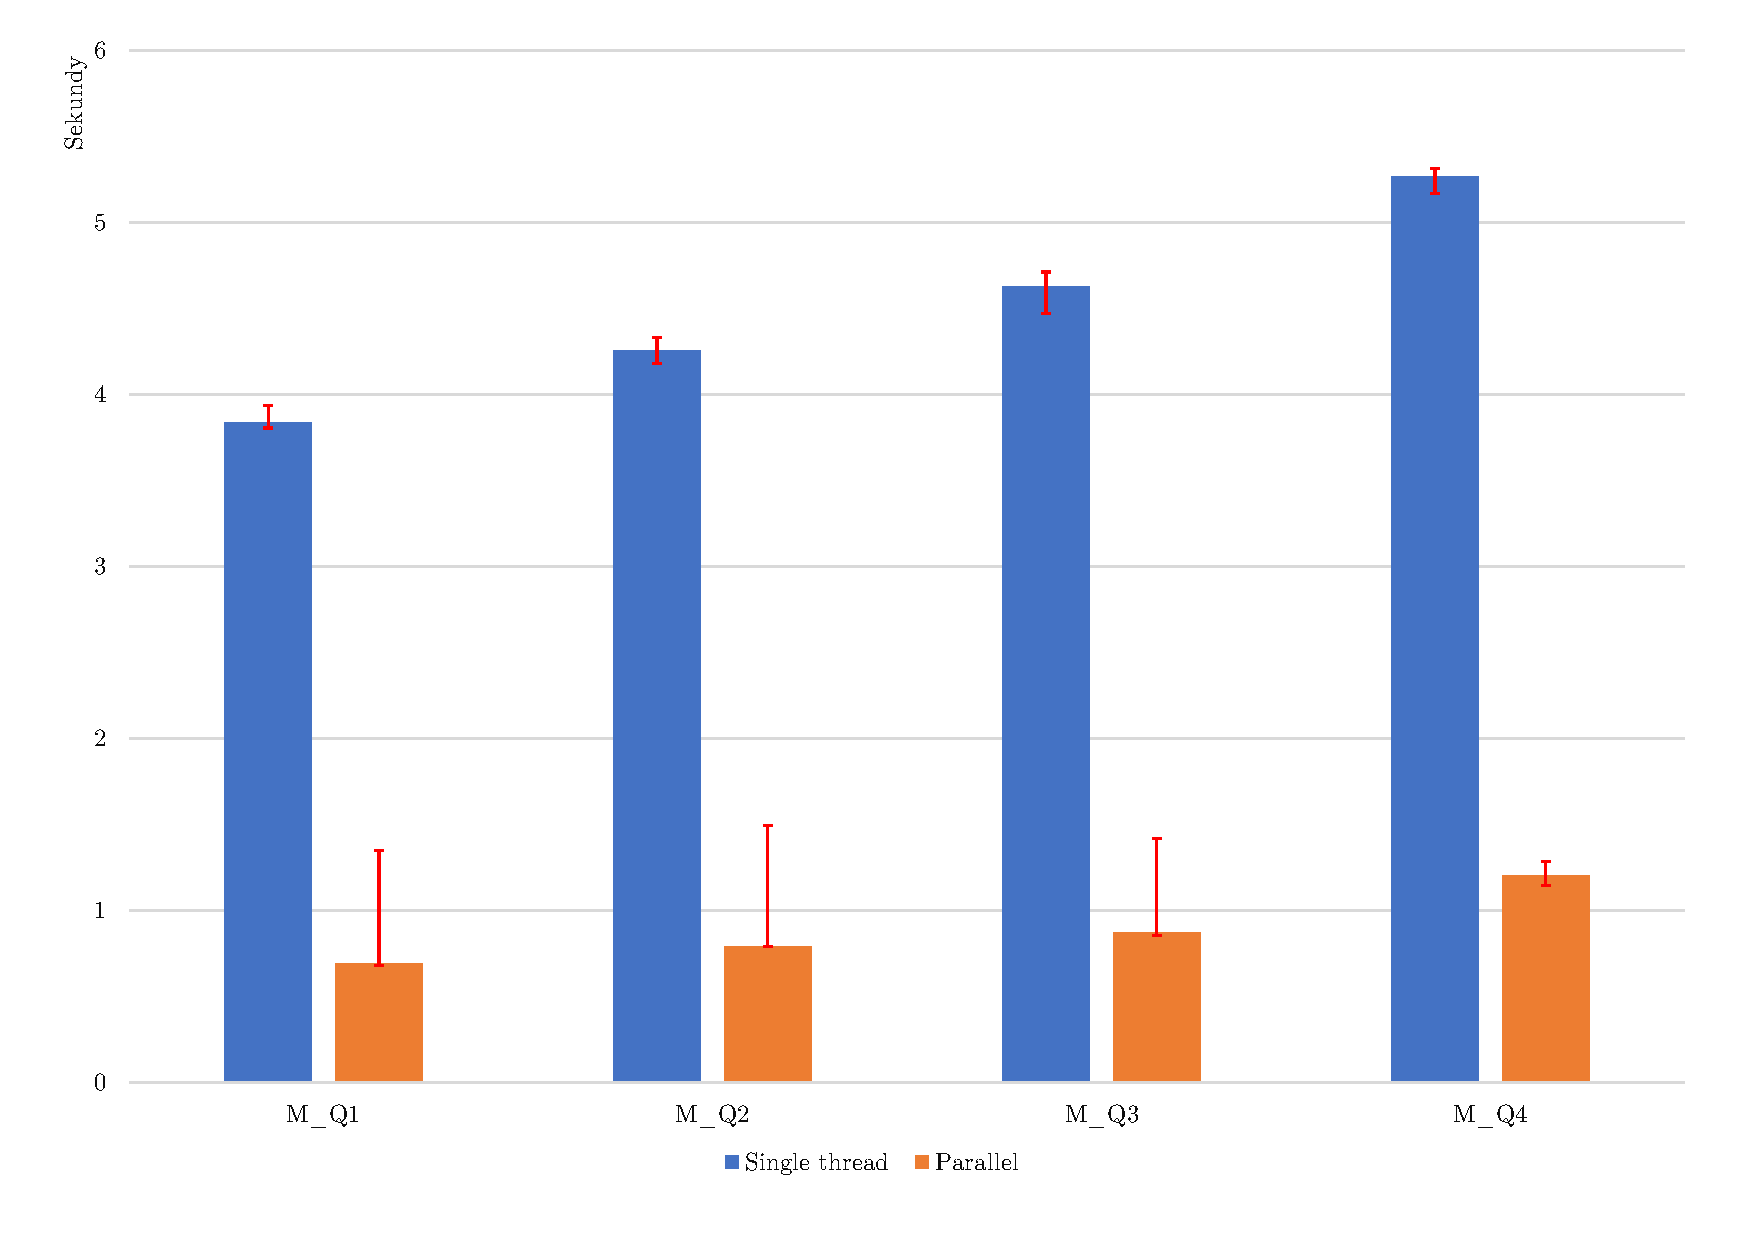
\includegraphics[width=\linewidth]{../img/amazonMatch.pdf}\centering
\caption{Doba vykonání dotazů \textit{Match} pro graf Amazon0601 (sekce \ref{tab.grafBase}). Jedno vlákno vůči osmi vláknům.}
\label{figure.amazonMatch}
\end{figure}

\begin{figure}[!htp]
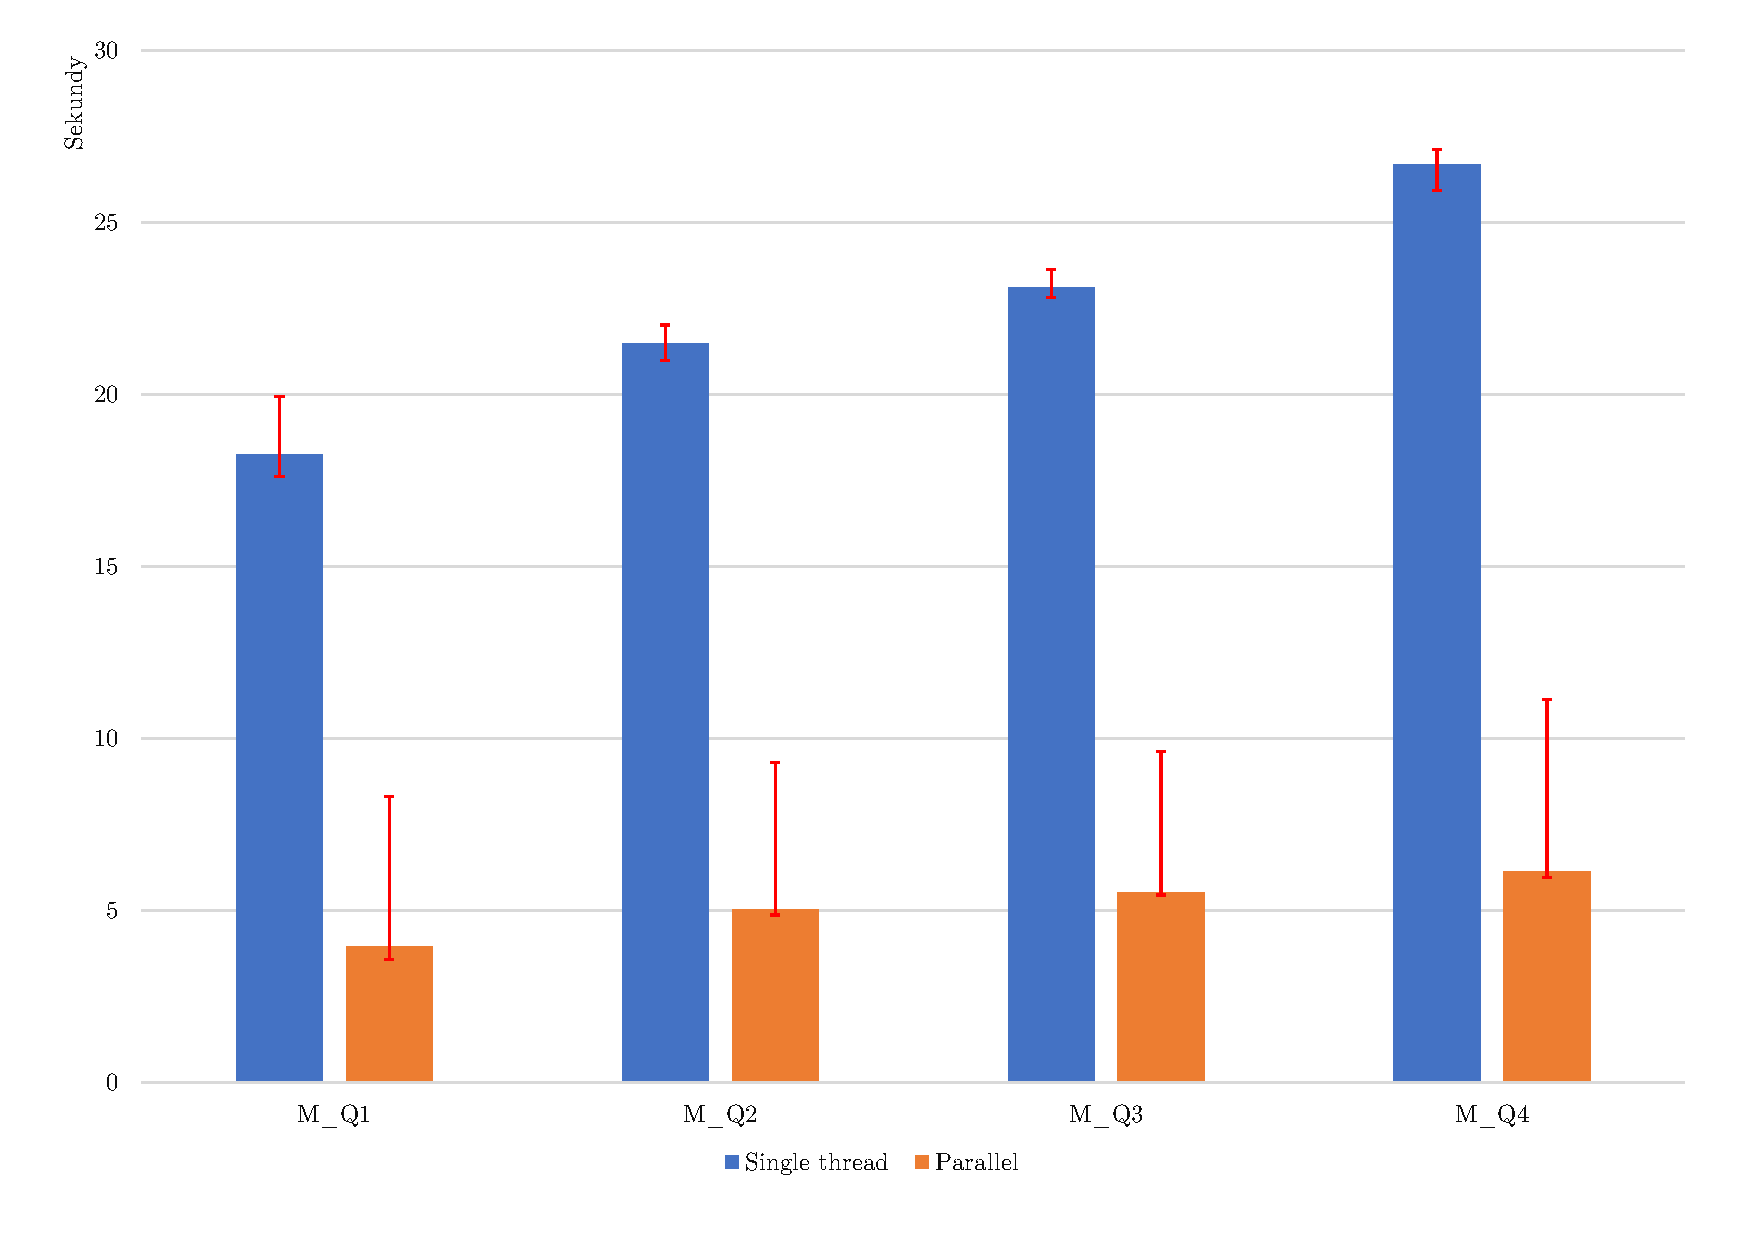
\includegraphics[width=\linewidth]{../img/webberkstanMatch.pdf}\centering
\caption{Doba vykonání dotazů \textit{Match} pro graf WebBerkStan (sekce \ref{tab.grafBase}). Jedno vlákno vůči osmi vláknům}
\label{figure.webberkstanMatch}
\end{figure}

\begin{figure}[!htp]
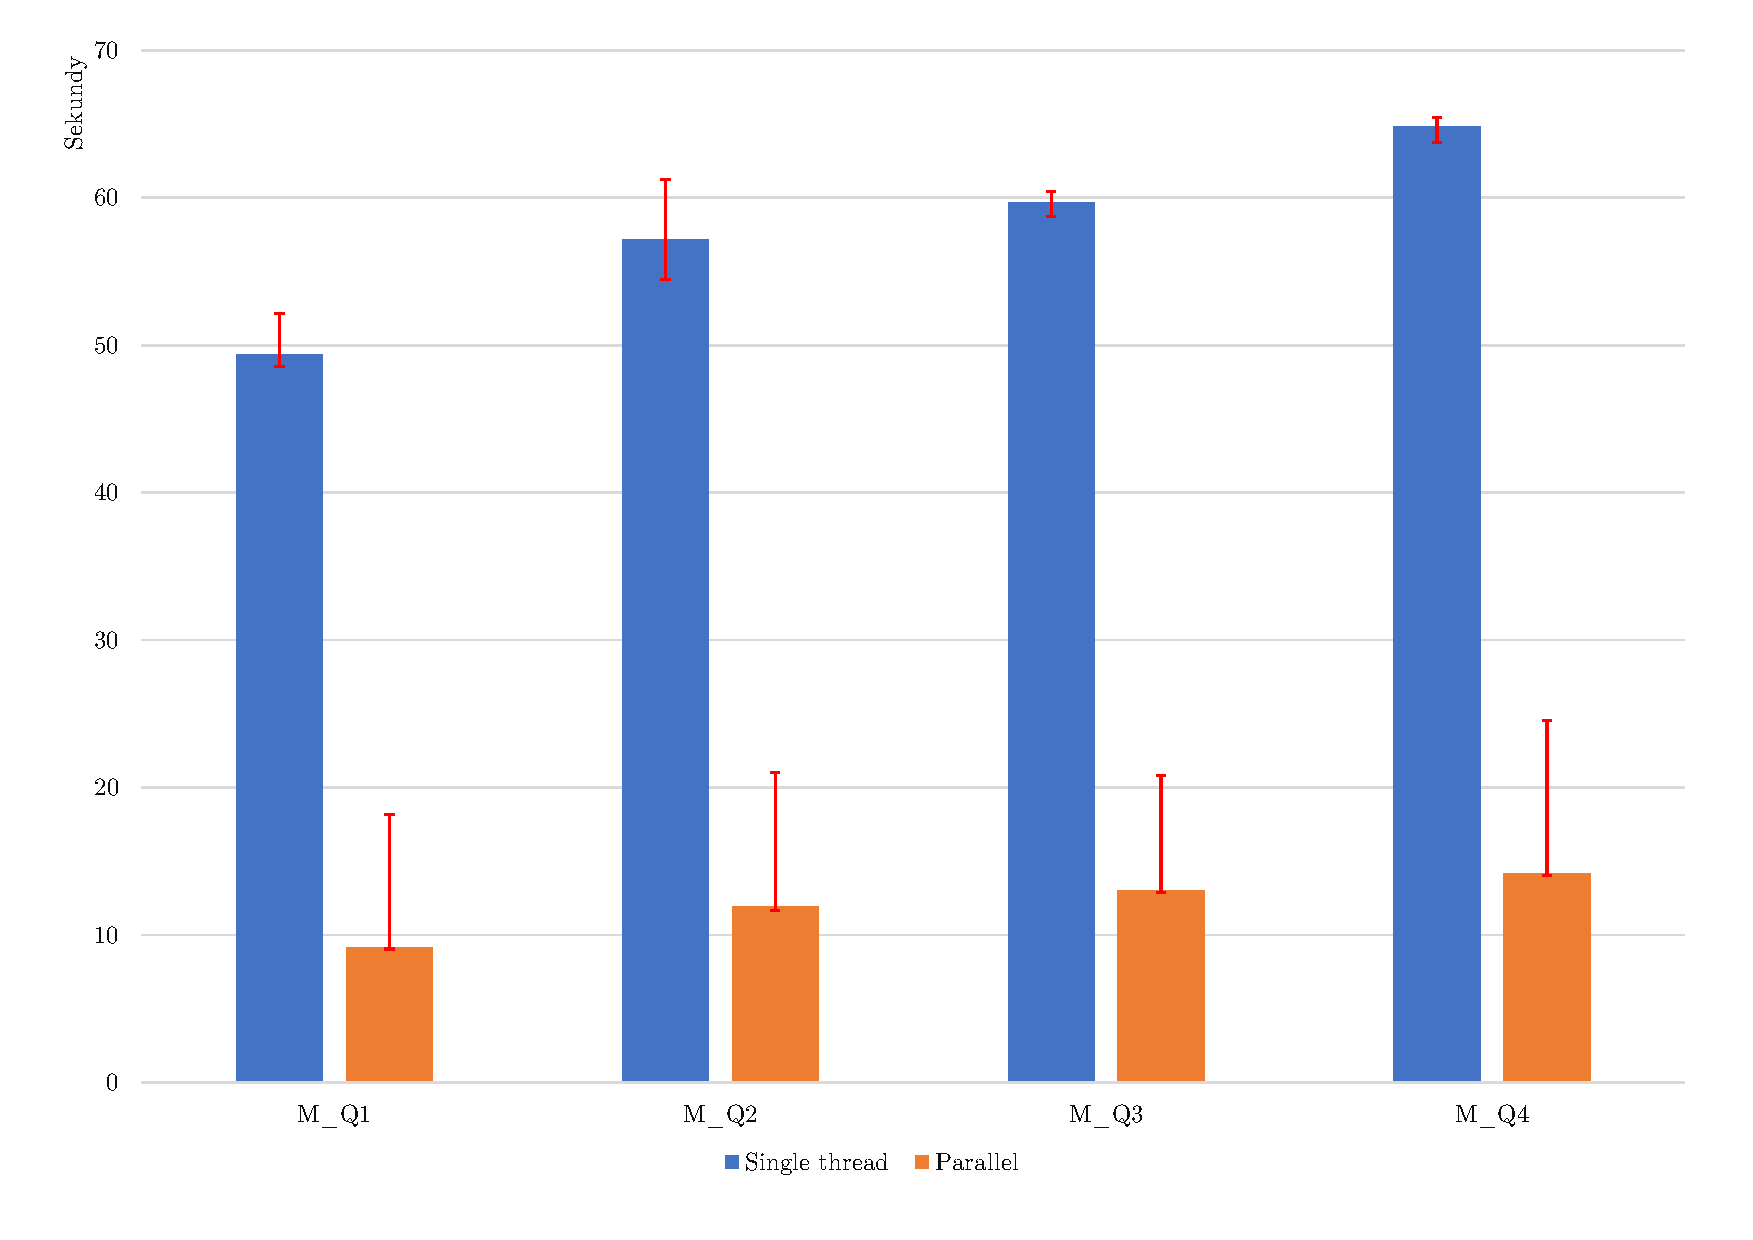
\includegraphics[width=\linewidth]{../img/skitterMatch.pdf}\centering
\caption{Doba vykonání dotazů \textit{Match} pro graf As-Skitter (sekce \ref{tab.grafBase}). Jedno vlákno vůči osmi vláknům.}
\label{figure.skitterMatch}
\end{figure}


\subsection{Order by}

Z důvodu časové a prostorové složitosti třídění na grafu As-Skitter jsme se rozhodli jej vynechat pro \textit{Order by} dotazy.
Všechny výsledky měření třídění jsou zobrazeny na grafech na konci této sekce.

\subsubsection{Obecné shrnutí jednovláknových řešení}

Nejprve shrneme základní koncepty použitých řešení.
Každé řešení pracuje s tabulkou výsledků, kterou musí setřídit.
Nikdy netřídíme samotné řádky tabulky, ale pouze indexy řádků.
Výsledek třídění je indexační struktura nad tabulkou.
Při porovnávání je nutné mít na paměti, že jednovláknově běžící části používají optimalizace popsané v sekcích \ref{anal.orderby.opt1}, \ref{anal.orderby.opt2} a \ref{impl.orderby.opts}.  

Mód \textbf{Normal} využívá k třídění algoritmus Merge sort.
Algoritmus je implementován v knihovně HPCsharp \citep{hpcsharp}.
Třídění probíhá po dokončení prohledávání grafu a třídí celou tabulku výsledků pomocí pole indexů.

Vylepšená řešení zpracovávají vyhledané výsledky v moment jejich nalezení.
Nalezený prvek se nejdříve vloží do tabulky na nový řádek. 
Následně se index daného řádku vloží do indexační struktury. 
Jako indexační strukturu nad tabulkou používáme $(a, b)$-strom \citep[str. 190]{labyrint}, u kterého jsme upravili definici na $b=2a$.
V našem případě $b=256$.
V řešení \textbf{ABTree} se jedná o obecný $(a, b)$-strom, zatímco řešení \textbf{ABTreeValueAccumulator} výsledky (indexy) mající stejnou hodnotu klíčů třídění jako již vložené prvky uloží do \verb+List<int>+.
Tedy místo vytvoření nového záznamu ve stromě dojde pouze k vložení do patřičného pole.

\subsubsection{Výsledky jednovláknového zpracování}

Začneme řešením běžícím v jednom vlákně, tj. grafy \ref{figure.amazonOrderST} a \ref{figure.webberkstanOrderST}.
Můžeme si všimnout, že výsledky vypadají v rámci daných grafů konzistentně pro každý dotaz.
Ani jedno z vylepšených řešení nedokázalo porazit mód \textbf{Normal}. 
Je to způsobeno značnou režií za metodu vložení (\verb+Insert+) do stromu, ve které dochází k častému alokování nových vrcholů a překopírovávání prvků.
Nejproblematičtější část je množství tříděných výsledků, kdy počet samotných hodnot klíčů třídění je omezen počtem vrcholů v grafu (tabulka \ref{tab.grafBase}). 
Daná situace vede k opakovanému zatřiďování výsledků se stejnou hodnotou a tím navyšování velikosti stromu společně s počtem vykonaných porovnání v metodě \verb+Insert+.
Celý problém jsme vyřešili v řešení \textbf{ABTreeValueAccumulator}, ve kterém se duplicitní hodnoty ukládají do zmíněného pole a tím omezujeme velikost výsledného stromu. 
Jak vidíme na grafech, řešení se přibližuje rychlosti řešení \textbf{Normal}.
Problém by nastal v případě, pokud by množství hodnot odpovídalo počtu nalezených výsledků. 
V tomto případě bychom zbytečně navyšovali režii za vzniklá pole, která se nevyužijí.

\subsubsection{Třídění pomocí vlastnosti vůči \texttt{ID}}

Dle našich předpokladů se ukázalo, že třídění pomocí vlastnosti (O\_Q3 a O\_Q4) vůči \verb+ID+ (O\_Q1 a O\_Q2) vede ke znatelnému zpomalení.
Je to způsobeno nutným přístupem k databázi, při kterém se ověřuje, jestli daná vlastnost existuje na daném elementu a následném čtení hodnoty ze struktury obsahující ji.

\subsubsection{Obecné shrnutí paralelních řešení}

Opět zde platí, že tabulka výsledků je tříděna pomocí indexů.
Mód \textbf{Normal} používá paralelní Merge sort \citep{hpcsharp}.
Vylepšená paralelní zpracování aplikují použité verze $(a, b)$-stromů ze zpracování pro jedno vlákno. 
Každé běžící vlákno v \textbf{Half-Streamed} řešení obsahuje lokální tabulku a indexační strom. 
Po dokončení vyhledávání se obsahy stromů překopírují do pole a dojde k paralelnímu dvoucestnému slévání používající stejnou funkci jako paralelní Merge sort. 
U \textbf{Streamed} řešení jsme navrhli sdílenou strukturu pro zatřiďování výsledků.
Struktura rozdělí rozsah hodnot prvního klíče třídění na rovnoměrné části (konkrétněji v sekci \ref{anal.improvement.orderby.streamed})
Počet částí je heuristicky zvolen jako $m=t^2$, kde $t=\#vláken$. 
Pro každou část rozsahu vytvoříme přihrádku obsahující zámek, tabulku a indexační strom.
Při příchozím výsledku se získá hodnota prvního klíče třídění a určí se jeho patřičná přihrádka. 
Do přihrádky vlákno přistoupí pomocí přiloženého zámku.
Následně výsledek vloží do tabulky a index nového řádku tabulky do stromu.
Rozdíl v řešeních je pak jen využitá stromová struktura.
Při porovnávání je nutné mít na paměti, že lokálně běžící části používají optimalizace popsané v sekcích \ref{anal.orderby.opt1}, \ref{anal.orderby.opt2} a \ref{impl.orderby.opts}.  

\subsubsection{Výsledky paralelního zpracování}

Nyní budeme prezentovat výsledky paralelizace (grafy \ref{figure.amazonOrderPar} a \ref{figure.webberkstanOrderPar}).
Na první pohled jsme si všimli mnohonásobného zpomalení \textbf{Streamed} řešení pro dotazy O\_Q1 a O\_Q2.
Výše jsme zmínili základní princip \textbf{Streamed} řešení.
Rozsah hodnot prvního klíče třídění se rozdělí na rovnoměrné části a pro každý takový rozsah existuje přihrádka přístupná pomocí zámku.
Vlákno v moment nalezení výsledku přistupuje k přihrádce pomocí zámku a vloží do ní daný výsledek.
Při implementaci řešení jsme se omezili pouze na celý rozsah hodnot typů vlastností v jazyce C\# pro .NET Framework 4.8.
To znamená, že pokud vlastnost má typ \texttt{integer} (v C\# \texttt{Int32}), ačkoliv hodnoty vlastnosti v grafu mohou být v rozsahu $[0; 100]$, tak rozdělení přihrádek se vytvářejí z celého rozsahu C\# typu.
Tedy přihrádky se vytvářejí rozdělením rozsahu $[$\verb+Int32.MinValue+; \verb+Int32.MaxValue+$]$ a nikoliv $[0; 100]$.
To má za následek při třídění pomocí vlastnosti s rozsahem hodnot v grafu $[0; 100]$, že vlákna budou přistupovat v nejhorším případě k pouze jedné přihrádce.
Vlákna pak budou vždy čekat na uvolnění jednoho zámku.
Přesně tato situace nastala u \textbf{Streamed} řešení pro dotazy O\_Q1 a O\_Q2.
V nich třídíme pomocí vlastnosti \texttt{ID}. 
\texttt{ID} je typu \texttt{integer}.
Vlastnost typu \texttt{integer} je v C\# typ \texttt{Int32}.
Vytvoří se přihrádky rozdělením rozsahu $[$\verb+Int32.MinValue+; \verb+Int32.MaxValue+$]$.
Rozsah se rozdělí na 64 dílů, protože jsme určili počet přihrádek jako $m=t^2$, kde $t=\#vláken$ a všechny testy běží v osmi vláknech.
Ale problém je, že hodnoty \texttt{ID} vrcholů jsou z omezeného rozsahu $[0; \#$vrcholů v grafu$]$, zatímco pouze jedna přihrádka obsahuje posloupnost 67 108 863 hodnot.
A vždy platí, že 67 108 863 $> \# $vrcholů v grafu (z tabulky \ref{tab.grafBase}).
Čili vlákna vždy přistupují pouze k přihrádce, kde se synchronizují pomocí zámku. 
Výsledná doba zpracování pak odpovídá jednovláknovému zpracování s přidanou režií za přístup k zámku.

Naopak u dotazů O\_Q3 a O\_Q4 je tříděno pomocí hodnot vygenerovaných náhodně spadající do celého rozsahu typu klíče a zde \textbf{Streamed} řešení předčilo všechna ostatní. 
Jsme si vědomi, že rozdělení na základě celého rozsahu není ideální, ale chtěli jsme vyzkoušet, jestli daný přístup bude využitelný.
Pro budoucí rozšíření by bylo nutné zvážit vytvoření statistik rozsahů jednotlivých vlastností, aby bylo možné lépe vytvořit rozdělení přihrádek.

\subsubsection{Zrychlení paralelních řešení pro O\_Q3 a O\_Q4 }

\textbf{Half-Streamed} řešení se přibližuje \textbf{Normal} řešení v prvních dvou dotazech a překonává jej ve třetím i čtvrtém dotazu pro řešení  \textbf{ABTreeValueAccumulator}.
U třetího a čtvrtého dotazu se porovnává pomocí vlastností. V jednovláknovém zpracovávání jsme viděli režii za dané porovnání.
V druhém kroku u daného \textbf{Half-Streamed} řešení dochází k slévání pouze akumulovaných skupin, což rapidně sníží počet porovnávání při slévání a odtud výhoda oproti \textbf{Normal: Merge sort} řešení. 
To samé platí u \textbf{Streamed} řešení, protože použití přihrádek způsobí vkládání do mnohonásobně menší skupiny výsledků. 
Celá situace je navíc umocněna zmíněnými optimalizacemi. 

\subsubsection{Rozsah zrychlení paralelních řešení}

Zajímavý výsledek testování je rozsah zrychlení vylepšených módů, tj. tabulky \ref{tab.OrderByZrychleniAmazon} a \ref{tab.OrderByZrychleniWebBerkStan}. 
Zrychlení Merge sortu zaostává. 
Maximální zrychlení u ostatních řešení je až pětinásobné. 
Danou situaci si vysvětlujeme následovně.
Implementace paralelního algoritmu Merge sort funguje na principu postupného rekurzivního rozdělování, při kterém se vytváří nové \verb+Tasks+ pro \verb+ThreadPool+.
U vylepšených řešení běží jedna metoda pro každé vlákno po dobu celého zpracování. 


\begin{figure}[!htp]
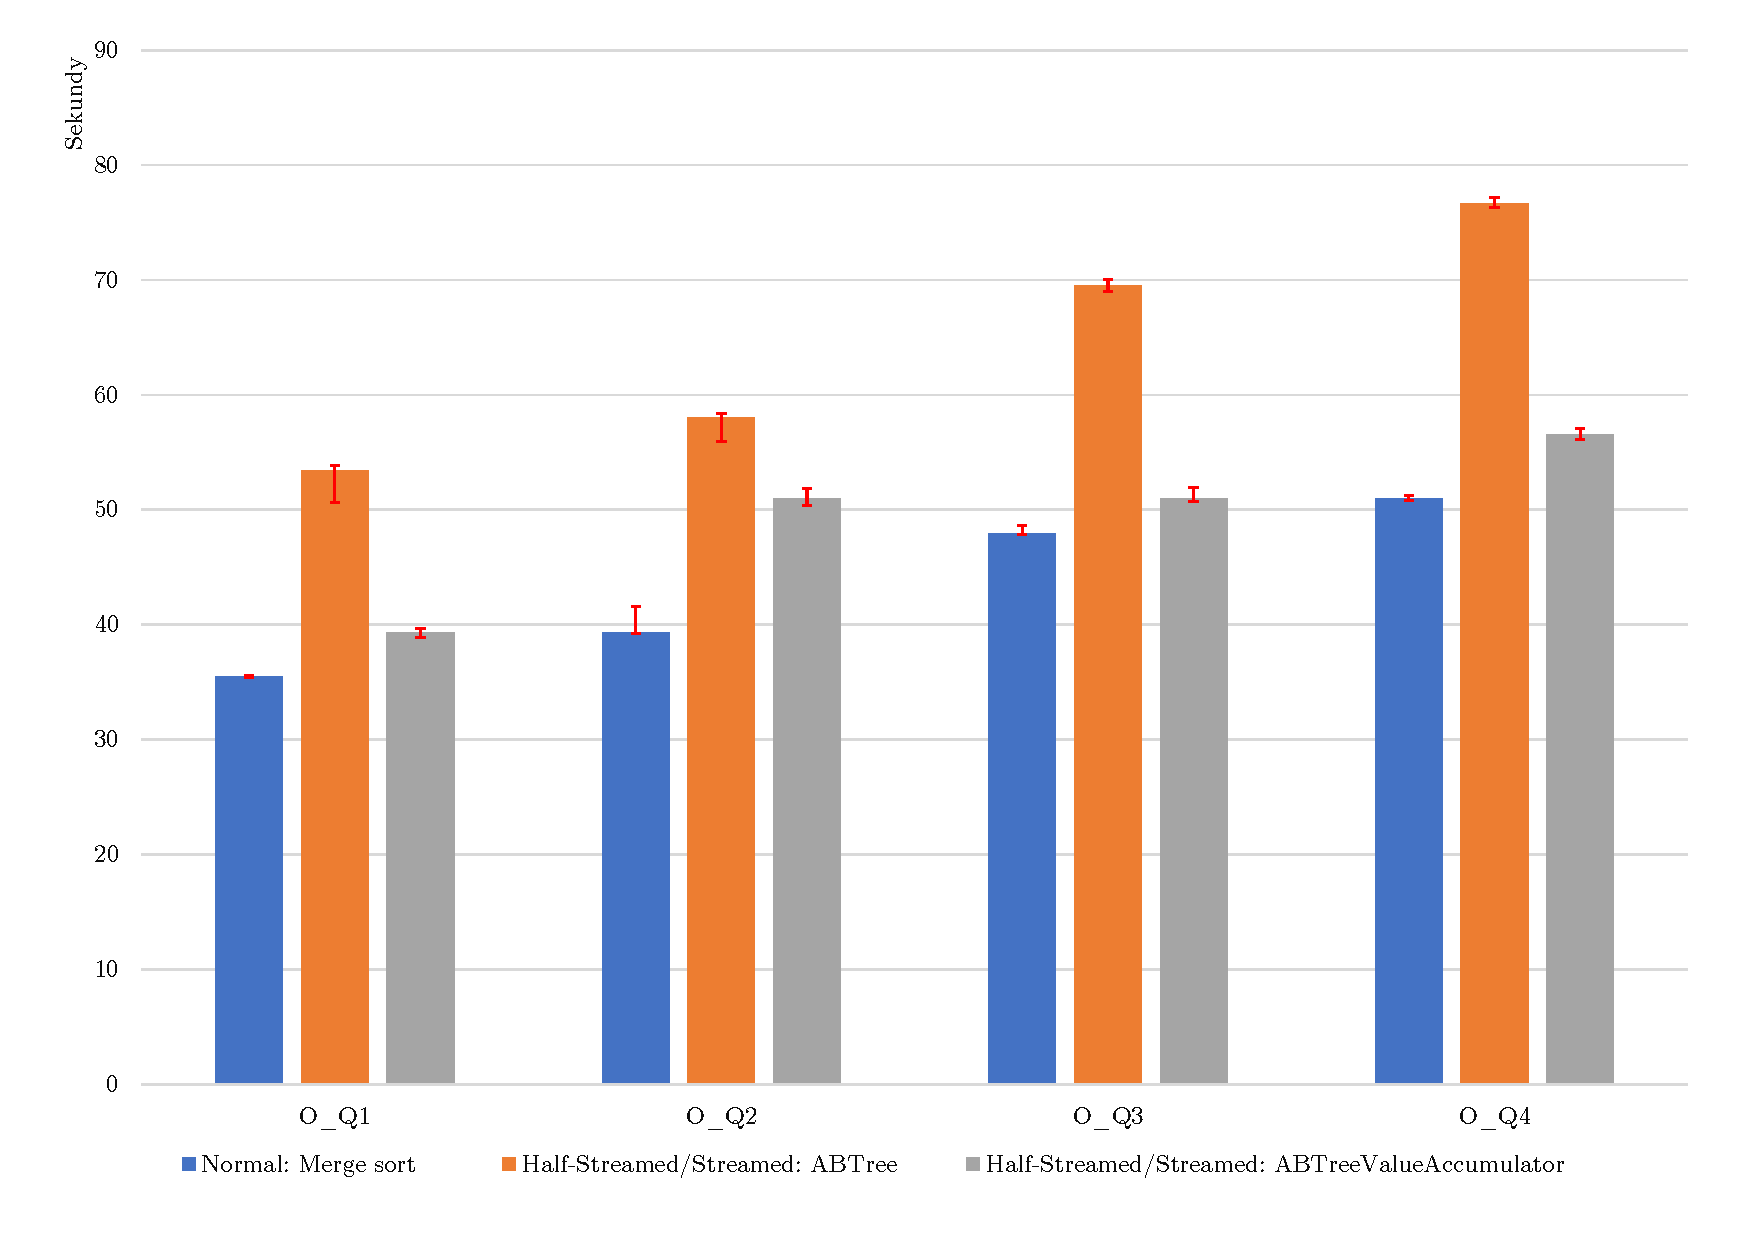
\includegraphics[width=\linewidth]{../img/amazonOrderByST.pdf}\centering
\caption{Doba vykonání dotazů \textit{Order by} pro graf Amazon0601 (sekce \ref{tab.grafBase}). Běh v jednom vláknu.}
\label{figure.amazonOrderST}
\end{figure}
\begin{figure}[!htp]
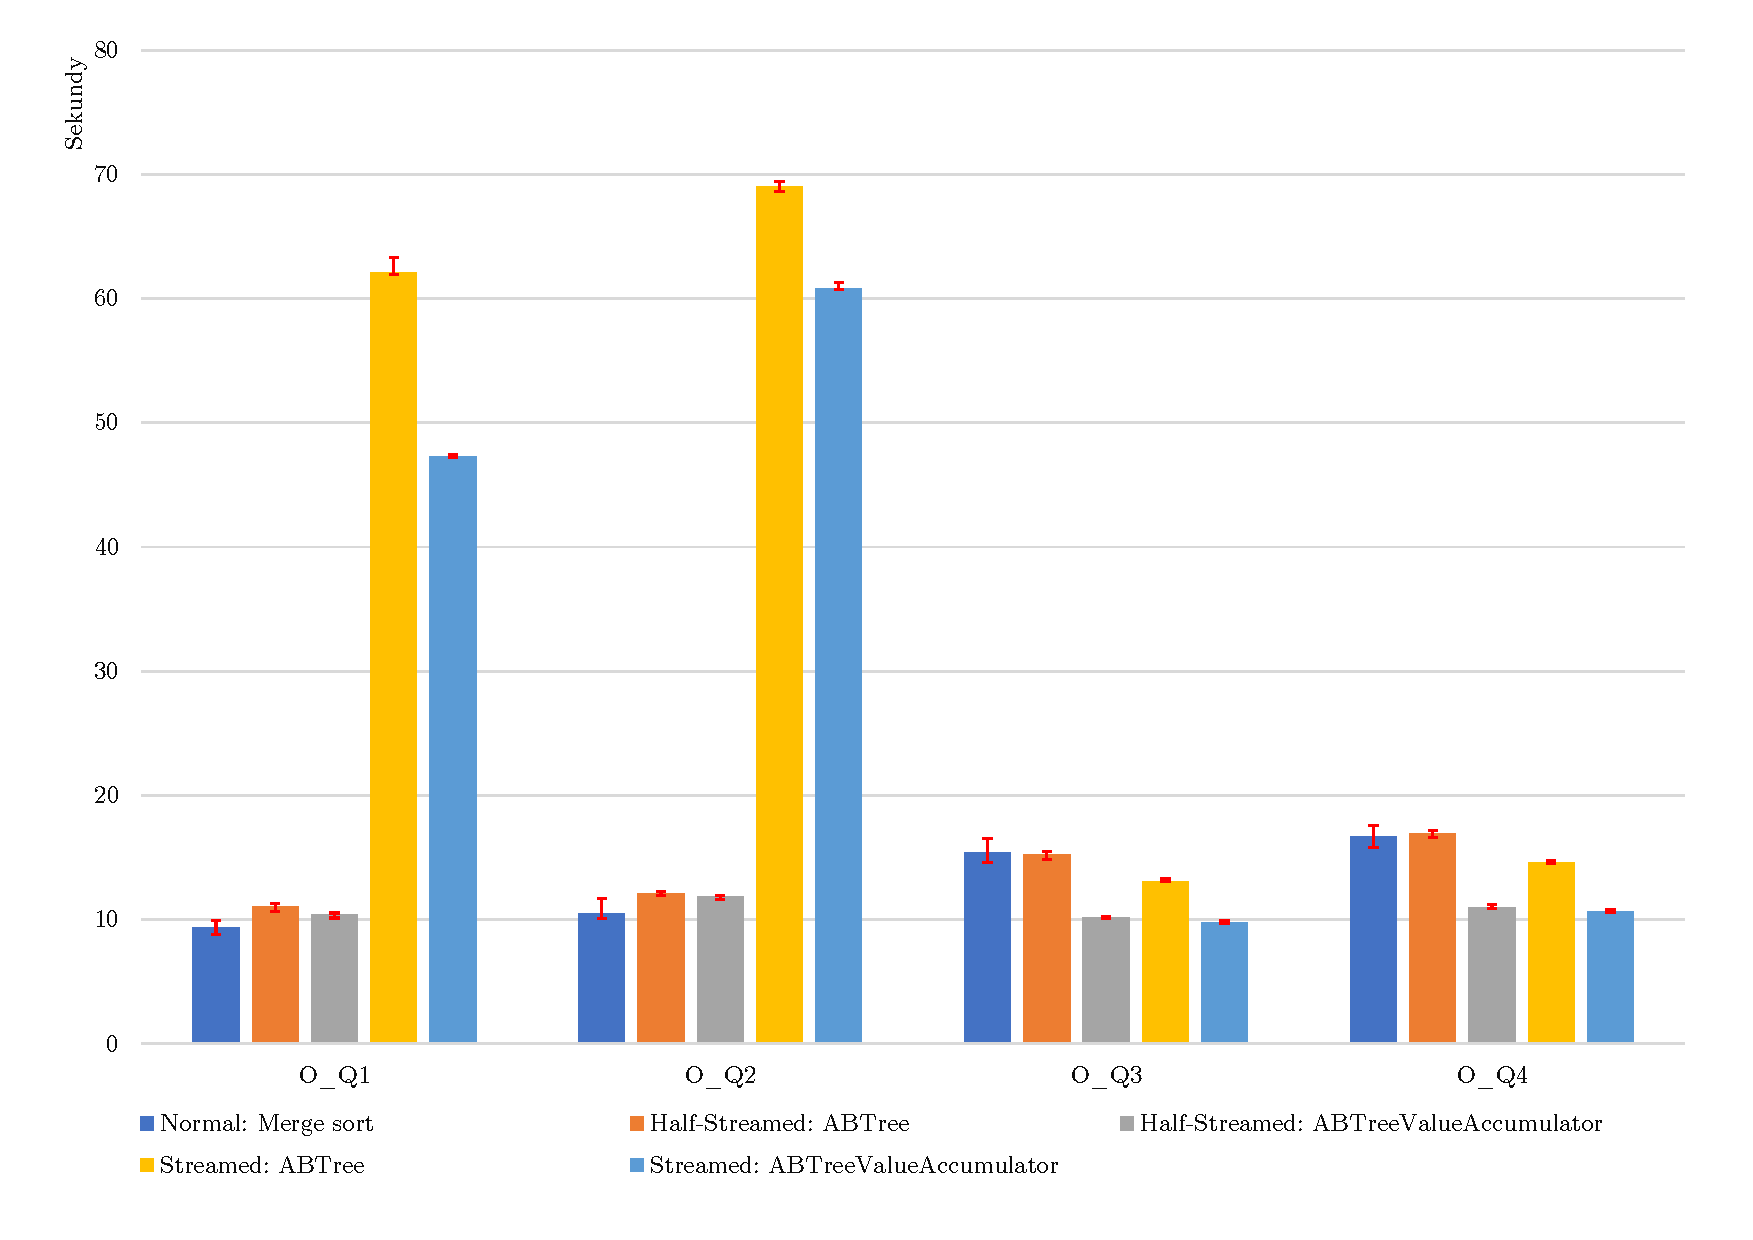
\includegraphics[width=\linewidth]{../img/amazonOrderByPar.pdf}\centering
\caption{Doba vykonání dotazů \textit{Order by} pro graf Amazon0601 (sekce \ref{tab.grafBase}).  Běh osmi vláken.}
\label{figure.amazonOrderPar}
\end{figure}

\begin{figure}[!htp]
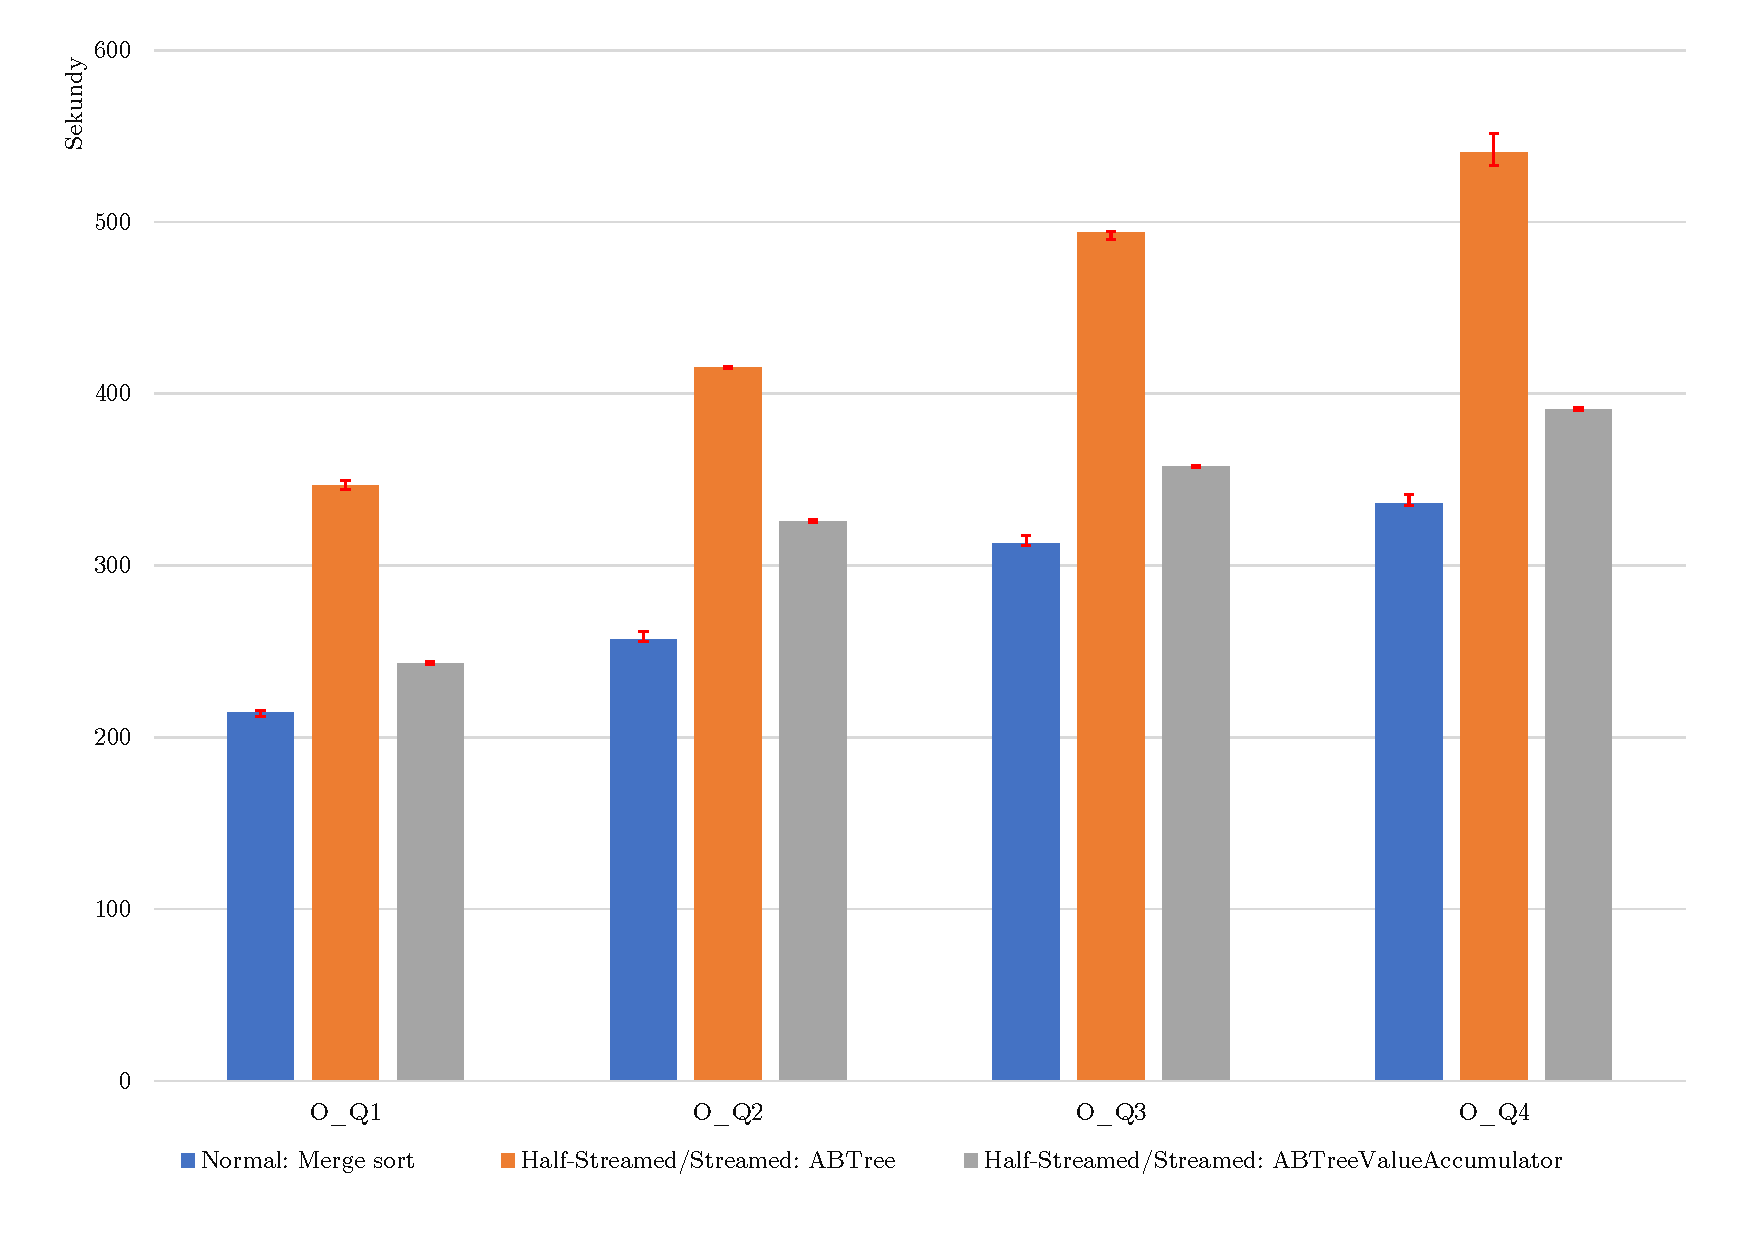
\includegraphics[width=\linewidth]{../img/webberkstanOrderByST.pdf}\centering
\caption{Doba vykonání dotazů \textit{Order by} pro graf WebBerkStan (sekce \ref{tab.grafBase}). Běh v jednom vláknu.}
\label{figure.webberkstanOrderST}
\end{figure}
\begin{figure}[!htp]
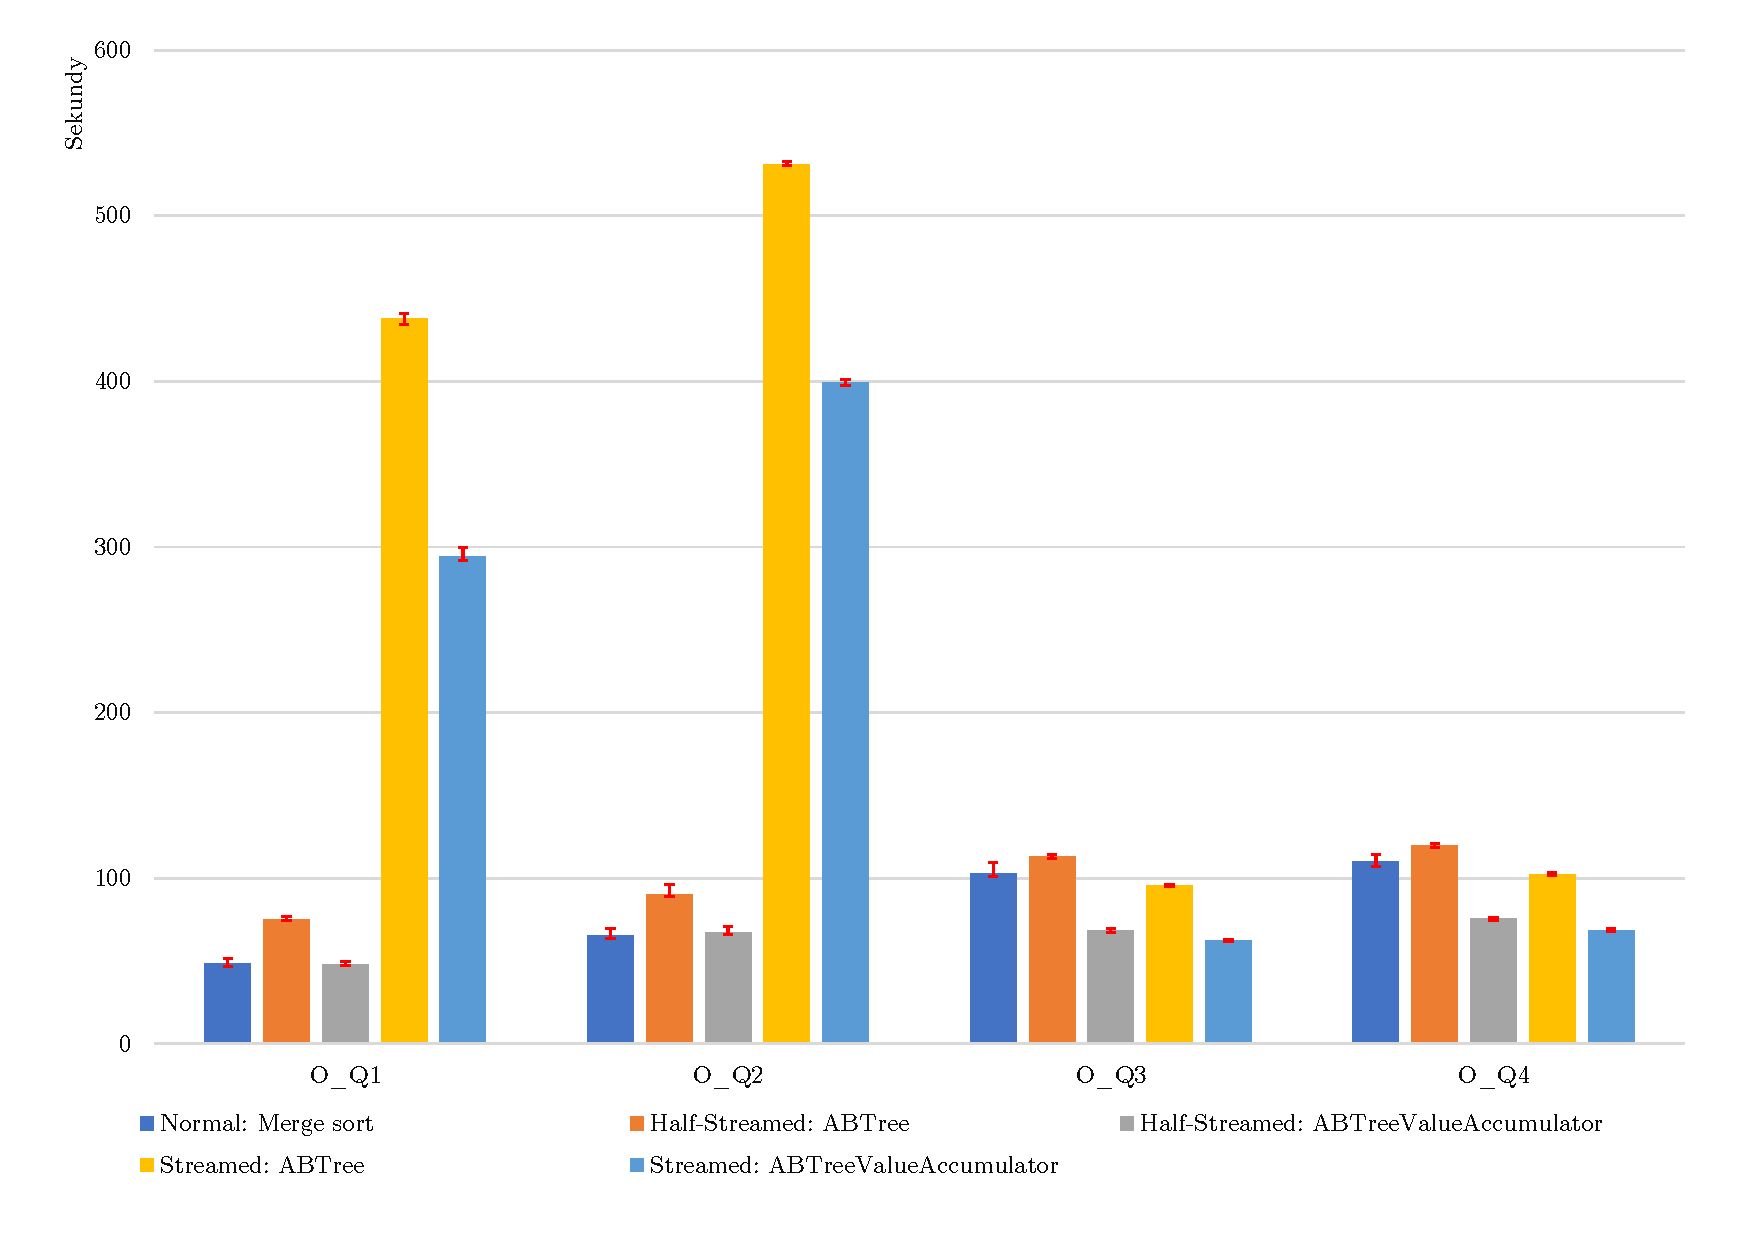
\includegraphics[width=\linewidth]{../img/webberkstanOrderByPar.pdf}\centering
\caption{Doba vykonání dotazů \textit{Order by} pro graf WebBerkStan (sekce \ref{tab.grafBase}).  Běh osmi vláken.}
\label{figure.webberkstanOrderPar}
\end{figure}

\clearpage

\begin{table}[!htb]
\centering
\begin{tabular}{lrrrr}
\toprule
\mc{} & \mc{O\_Q1} & \mc{O\_Q2} & \mc{O\_Q3} & \mc{O\_Q4} \\
\midrule
Normal: Merge sort                              & 3,79	& 3,75 &	3,12 &	3,05 \\
Half-Streamed: ABTree                   & 4,81	& 4,78 &	4,56 &	4,54 \\
Half-Streamed: ABTreeValueAccumulator   & 3,76	& 4,31 &	5,03 &	5,14 \\
Streamed: ABTree                        & 0,83	& 0,84 &	5,23 &	5,33 \\
Streamed: ABTreeValueAccumulator        & 0,86	& 0,84 &	5,30 &	5,25 \\ 
\bottomrule
\end{tabular}

\caption{Rozsah zrychlení paralelizovaných řešení pomocí osmi vláken pro dotazy \textit{Order by} nad grafem Amazon0601 (sekce \ref{tab.grafBase}). Tabulka zobrazuje podíl jednovláknového vůči paralelnímu zpracování.}
\label{tab.OrderByZrychleniAmazon}
\end{table}

\begin{table}[!htb]
\centering
\begin{tabular}{lrrrr}
\toprule
\mc{} & \mc{O\_Q1} & \mc{O\_Q2} & \mc{O\_Q3} & \mc{O\_Q4} \\
\midrule
Normal: Merge sort                              & 4,43	& 3,94	& 3,03 &	3,05 \\
Half-Streamed: ABTree                   & 4,59	& 4,61	& 4,36 &	4,51 \\
Half-Streamed: ABTreeValueAccumulator   & 5,05	& 4,83	& 5,21 &	5,18 \\
Streamed: ABTree                        & 0,83	& 0,82	& 5,72 &	5,72 \\
Streamed: ABTreeValueAccumulator        & 0,79	& 0,78	& 5,15 &	5,29 \\ 
\bottomrule
\end{tabular}

\caption{Rozsah zrychlení paralelizovaných řešení pomocí osmi vláken pro dotazy \textit{Order by} nad grafem WebBerkStan (sekce \ref{tab.grafBase}). Tabulka zobrazuje podíl jednovláknového vůči paralelnímu zpracování.}
\label{tab.OrderByZrychleniWebBerkStan}
\end{table}


Jako důsledek testování můžeme konstatovat, že třídění během prohledávání grafu v našich vybraných případech nepřináší zrychlení vykonávání.
Zrychlení nastává pouze u paralelizace řešení při dostatečně náhodném rozložení dat třídění, pokud je porovnáváno pomocí vlastností.
Zmínili jsme, že pro stromy nastává zpomalení kvůli režii za metodu \texttt{Insert}.
V našich vylepšeních jsme neimplementovali předalokování vrcholů stromu.
Jestli by pomocí předalokování nastalo zrychlení, které by předčilo řešení \textbf{Normal}, ponecháme jako budoucí rozšíření. 

\subsection{Group by}

\subsubsection{Obecné shrnutí jednovláknových řešení}

Než postoupíme dál, připomeneme hlavní rozdíly řešení a značení u zobrazených grafů. 
Každé řešení používá k \textit{Group by} mapu (\verb+Dictionary<key, value>+).
\textbf{Normal} řešení ukládá všechny výsledky vyhledávání vzoru do tabulky a po dokončení vykoná \textit{Group by}. 
\textbf{Half-Streamed} řešení vykonává \textit{Group by} v průběhu prohledávání a ukládá do tabulky pouze výsledky, pro které ještě neexistuje skupina v použité mapě.
Pro zmíněná řešení se jako \verb+key+ používá index do tabulky a skrze něj se následně vypočtou hodnoty klíče.
\textbf{Streamed} řešení nepoužívá tabulku, ale hodnoty klíče ukládá rovnou do mapy. 
Objevující se značení Bucket a List určuje způsob ukládání výsledků agregačních funkcí (\verb+min+, \verb+avg+...) jako \verb+value+ záznam v mapě.
Podrobnější vysvětlení je v kapitole Analýzy \ref{anal.groupby.uloziste}.
Výsledky jednovláknového seskupování jsou zobrazeny na grafech před shrnutím paralelních výsledků seskupování v sekci \ref{expr.results.groupby.par}.

\subsubsection{Výsledky jednovláknového zpracování}

Na grafech \ref{figure.amazonGroupByST}, \ref{figure.webberkstanGroupByST} a \ref{figure.skitterGroupByST} vidíme výsledky \textit{Group by} pro běh v jednom vlákně.
Výsledky na grafech \ref{figure.amazonGroupBySTNoAgg}, \ref{figure.webberkstanGroupBySTNoAgg} a \ref{figure.skitterGroupBySTNoAgg} představují dotazy bez agregačních funkcí v části \textit{Select}.
Dvě dvojice dotazů G\_Q4/G\_Q5, G\_Q2/G\_Q3 a trojice dotazů G\_Q6/G\_Q7/G\_Q8 jsou pouze mírně odlišné a můžeme u nich vidět konzistenci výsledků pro použité grafy.
Řešení vykonávající \textit{Group by} v průběhu vyhledávání překonávají \textbf{Normal} řešení.
S růstem počtu výsledku se rozdíly mezi módy prohlubují. 
Například zrychlení \textbf{Streamed} řešení je znatelnější u grafu As-Skitter než u grafu Amazon0601. 
Obecně nejznačnější zrychlení nastává u \textbf{Streamed} řešení, kdy není použita tabulka výsledků.

\subsubsection{Zpomalení jednovláknového Half-Streamed řešení}

Velice mírné zrychlení můžeme vidět u \textbf{Half-Streamed} řešení, které ukládá jen reprezentanty skupiny.
U všech dotazů bez agregačních funkcí, kromě dvojice G\_Q4$'$/G\_Q5$'$, nastávají situace, kdy \textbf{Half-Streamed} řešení je pomalejší než \textbf{Normal}.
U grafu Amazon0601 nastává stejná situace pro G\_Q3, G\_Q6 a pro každý graf pro G\_Q8.
Situaci jsme neočekávali a vysvětlujeme si ji následovně.
\textbf{Half-Streamed} řešení používá při zpracování výsledku položku tabulky \verb+temporaryRow+, do které přesouvá ukazatel na pole výsledků.
Skrze danou položku pak následně přistupuje k výsledku při vkládání do mapy. 
Na dané přesouvání se můžeme dívat jako na kopírování jedné proměnné do tabulky.
Při úspěšném vložení nastane navíc překopírování výsledků do pravé tabulky.
Což odpovídá větší režii na zpracování výsledku než u \textbf{Normal} řešení.
Proto vidíme pokles rychlosti a celkově jen mírné zrychlení u \textbf{Half-Streamed} řešení v jiných případech.
Největší skok pak právě nastává v dotazech G\_Q4/G\_Q4$'$ a G\_Q5/G\_Q5$'$, kdy se ukládají dvě proměnné.
Tedy samotná režie \textbf{Normal} řešení je značně pomalejší, protože musí ukládat vždy dvě proměnné, zatímco \textbf{Half-Streamed} jen přesouvá ukazatel.
Zajímavé je, že dané situace nastávají u dotazů bez agregačních funkcí, přestože všechna řešení pro jejich reprezentaci používají stejné funkce a struktury (List/Bucket).
Předpokládali bychom tedy stejnou situaci i na ostatních (větších) grafech.
Absenci jevu neumíme plně objasnit.

\subsubsection{Porovnání výsledků úložišť List/Bucket jednovláknového zpracování}

Na největším grafu platí, že použité ukládání List je pomalejší než Bucket, kvůli indirekci navíc.
Na menších grafech rozdíly ustupují, a dokonce nastávají situace, kdy je List rychlejší. 
Přesněji u dotazů G\_Q4 a G\_Q5.
Přehození rolí si u nich vysvětlujeme režií za množství vytvářených polí (tj. hodně alokací, málo přístupů), které se vyrovná použité indirekci.
Na grafu Amazon0601 u G\_Q4 a G\_Q5 dotazů je \textbf{Streamed} řešení pomalejší než \textbf{Half-Streamed} s úložištěm List, protože také vytváří pole jako Bucket řešení (viz implementace \ref{impl.improvement.groupby.streamed}).
U dalších grafů je pak počet vytvářených polí mnohonásobně menší než počet přístupů k nim.

\bigskip
Z výsledků můžeme vyvodit, že vylepšená jednovláknová \textbf{Streamed} řešení \textit{Group by} jsou výhodnější z hlediska rychlosti vykonávání než řešení \textbf{Normal}. 

\begin{figure}[!htp]
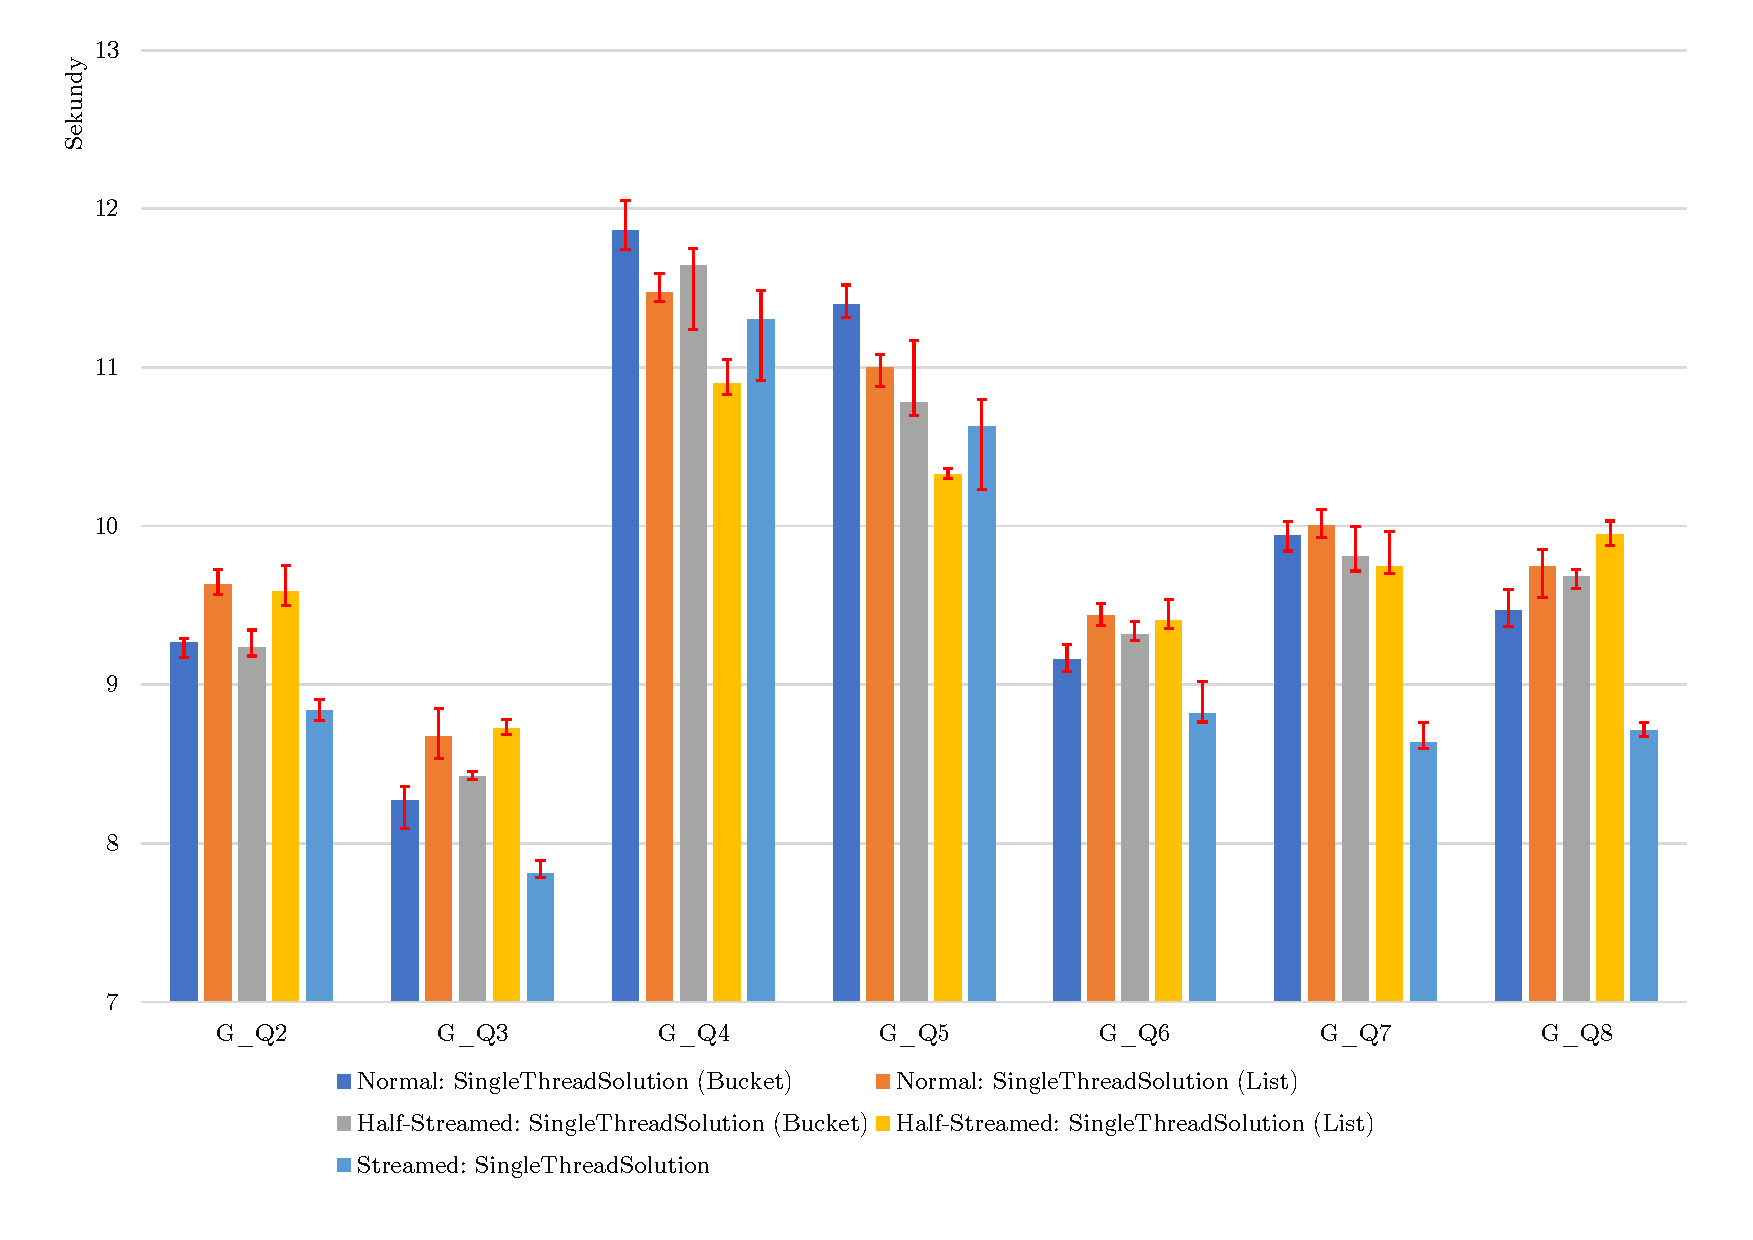
\includegraphics[width=\linewidth]{../img/amazonGroupByST.pdf}\centering
\caption{Doba vykonání dotazů \textit{Group by} pro graf Amazon0601 (sekce \ref{tab.grafBase}). Běh v jednom vláknu.}
\label{figure.amazonGroupByST}
\end{figure}
\begin{figure}[!htp]
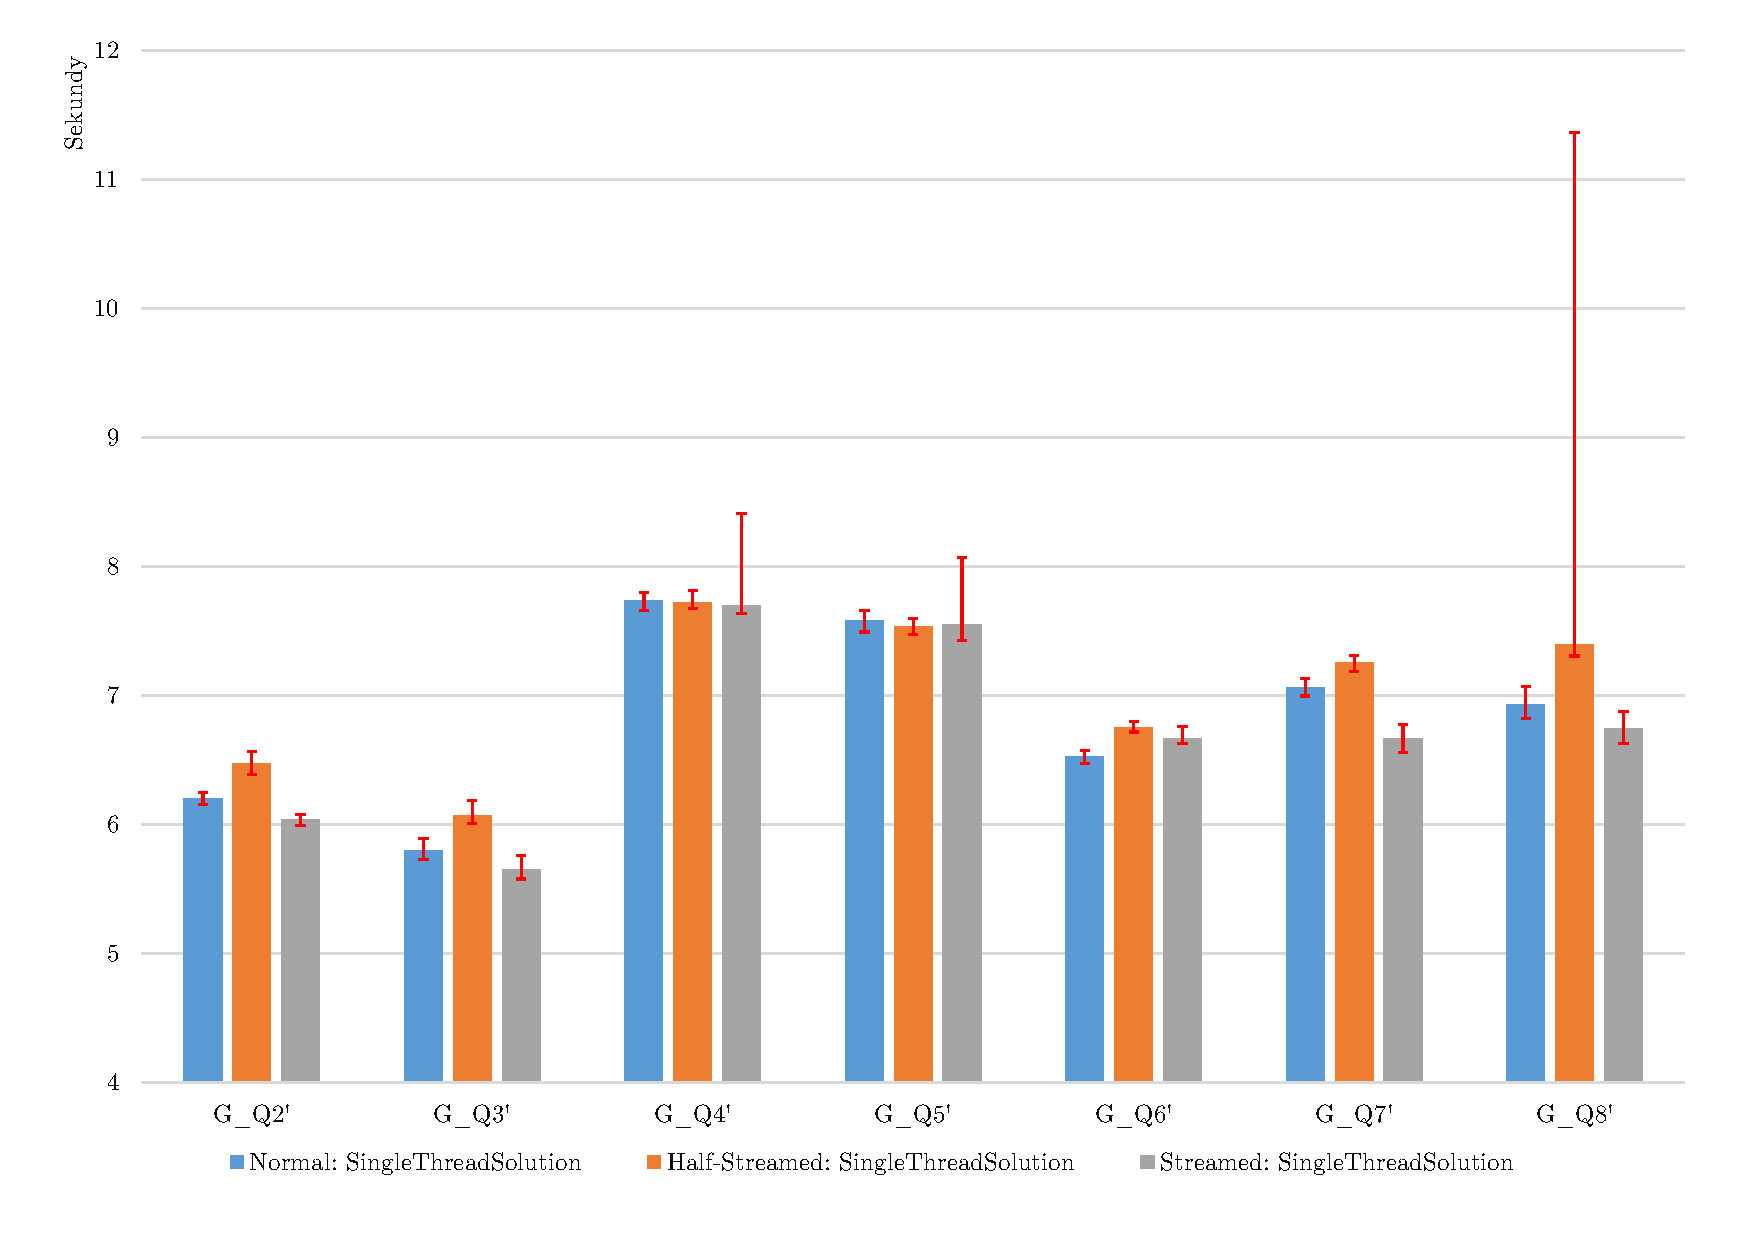
\includegraphics[width=\linewidth]{../img/amazonGroupBySTNoAgg.pdf}\centering
\caption{Doba vykonání dotazů \textit{Group by} pro graf Amazon0601 (sekce \ref{tab.grafBase})  bez agregačních funkcí. Běh v jednom vláknu.}
\label{figure.amazonGroupBySTNoAgg}
\end{figure}

\begin{figure}[!htp]
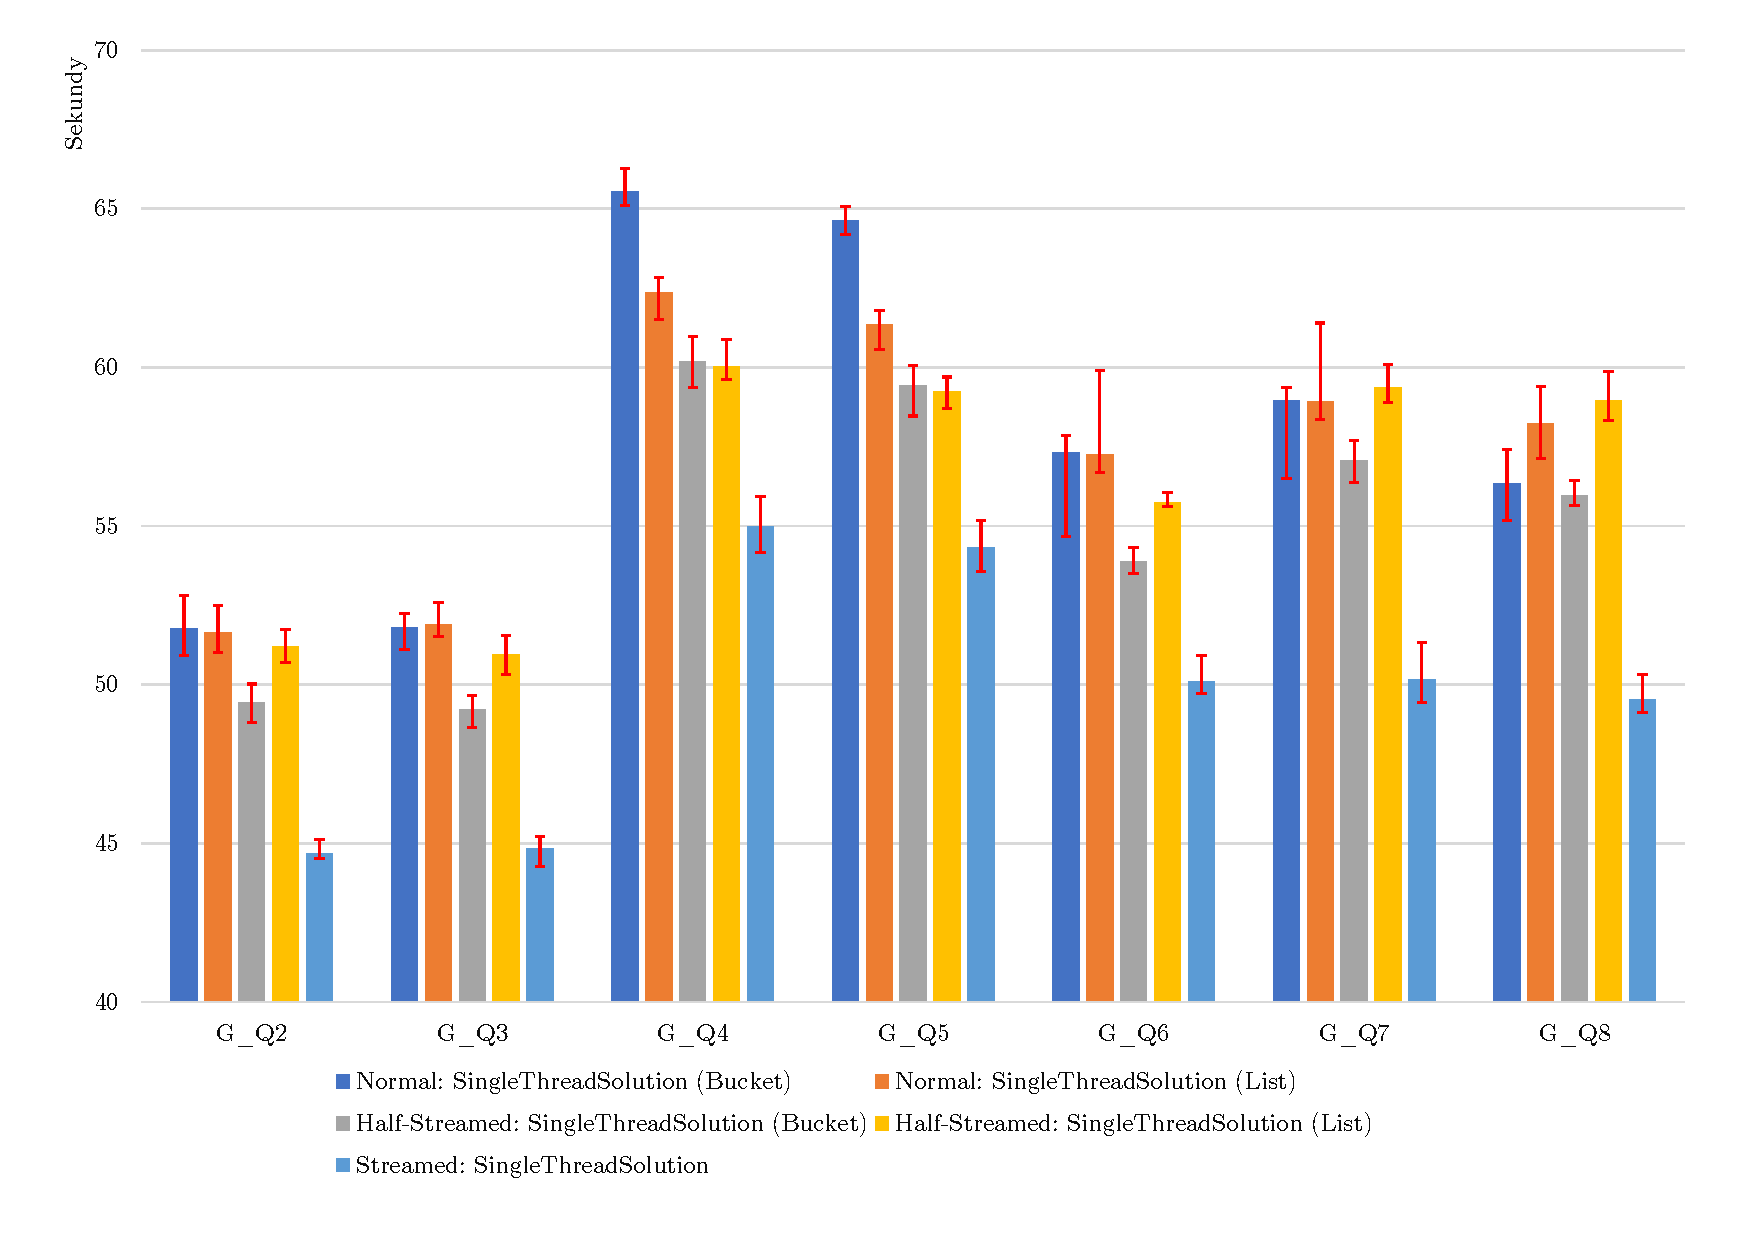
\includegraphics[width=\linewidth]{../img/webberkstanGroupByST.pdf}\centering
\caption{Doba vykonání dotazů \textit{Group by} pro graf WebBerkStan (sekce \ref{tab.grafBase}). Běh v jednom vláknu.}
\label{figure.webberkstanGroupByST}
\end{figure}
\begin{figure}[!htp]
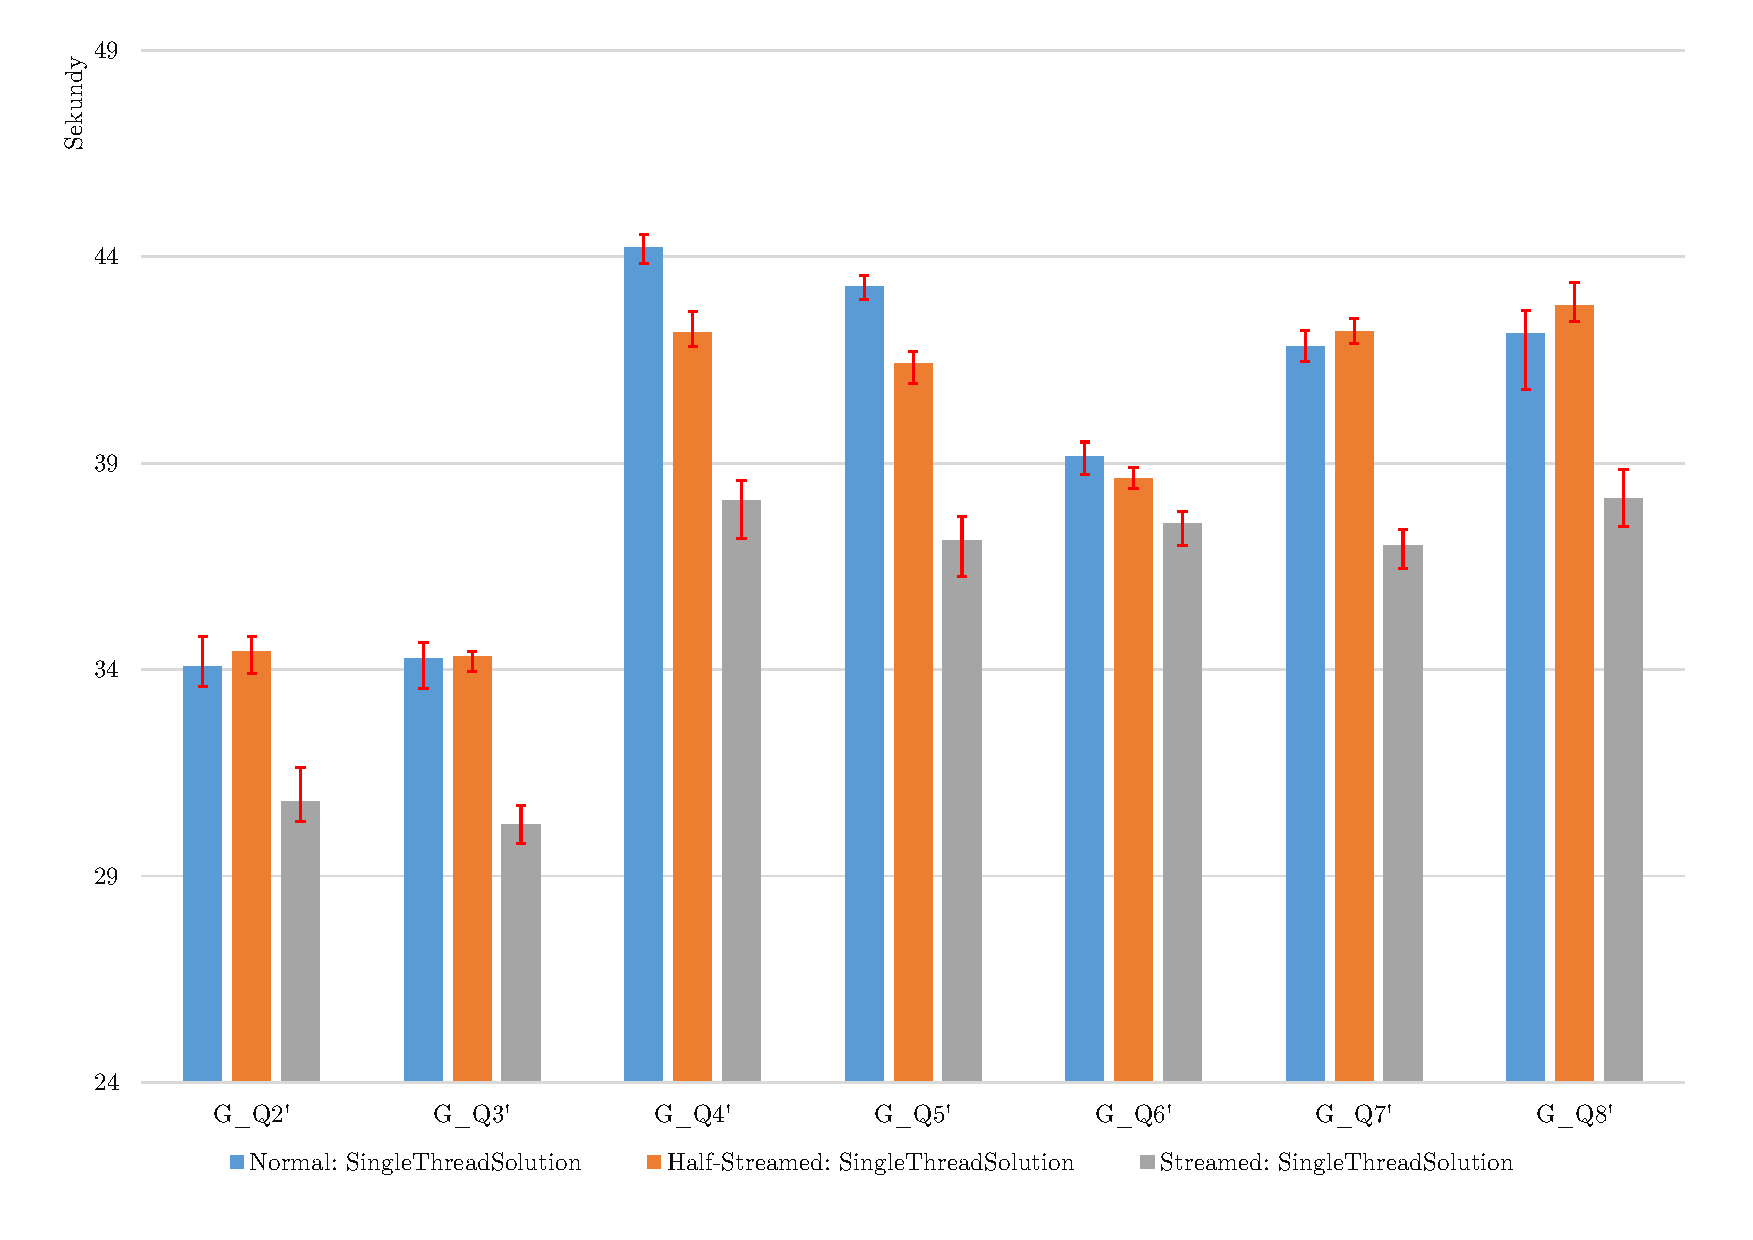
\includegraphics[width=\linewidth]{../img/webberkstanGroupBySTNoAgg.pdf}\centering
\caption{Doba vykonání dotazů \textit{Group by} pro graf WebBerkStan (sekce \ref{tab.grafBase}) bez agregačních funkcí. Běh v jednom vláknu.}
\label{figure.webberkstanGroupBySTNoAgg}
\end{figure}

\begin{figure}[!htp]
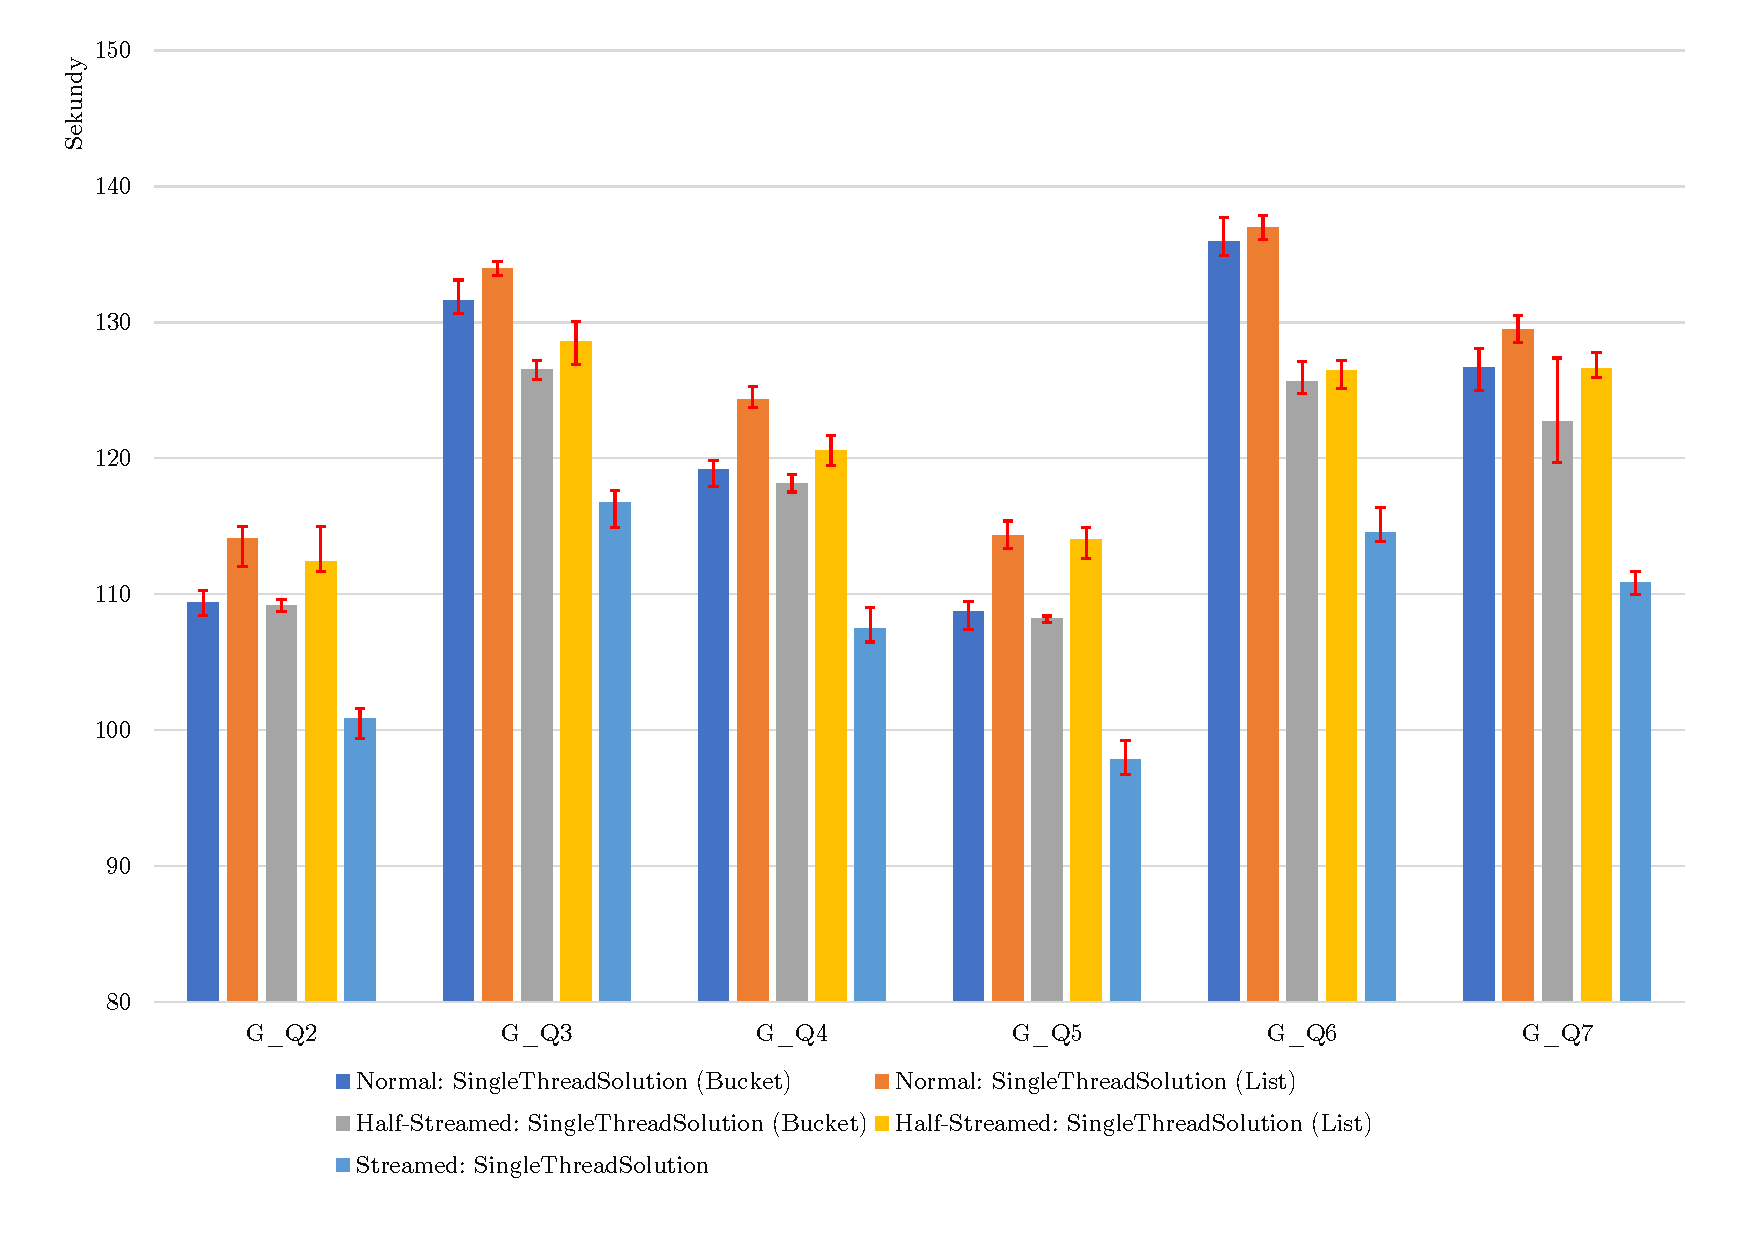
\includegraphics[width=\linewidth]{../img/skitterGroupByST.pdf}\centering
\caption{Doba vykonání dotazů \textit{Group by} pro graf As-Skitter (sekce \ref{tab.grafBase}). Běh v jednom vláknu.}
\label{figure.skitterGroupByST}
\end{figure}
\begin{figure}[!htp]
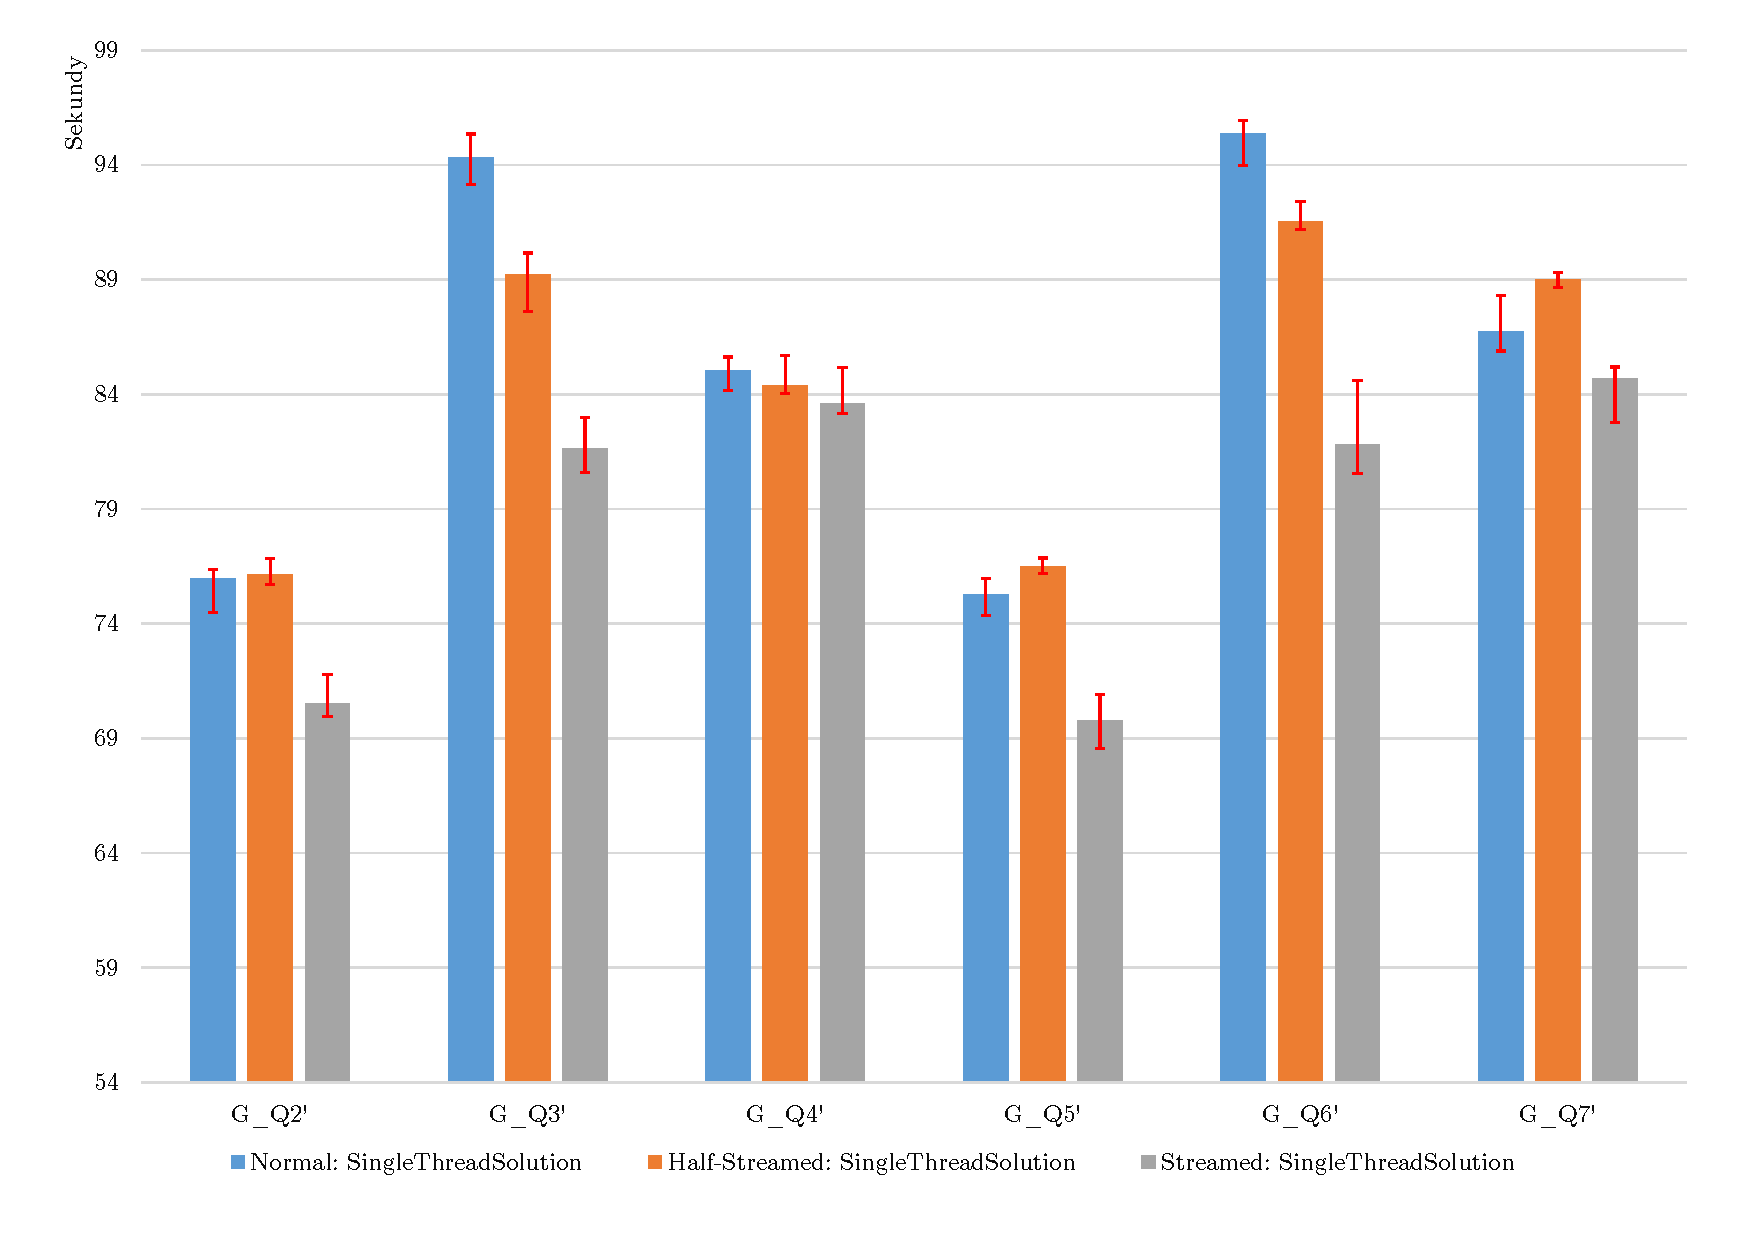
\includegraphics[width=\linewidth]{../img/skitterGroupBySTNoAgg.pdf}\centering
\caption{Doba vykonání dotazů \textit{Group by} pro graf As-Skitter (sekce \ref{tab.grafBase}) bez agregačních funkcí. Běh v jednom vláknu.}
\label{figure.skitterGroupBySTNoAgg}
\end{figure}


%%%%%%%%%%%%%%%%%%%%%%%%%%%%

\clearpage

\subsubsection{Obecné shrnutí paralelních řešení} \label{expr.results.groupby.par}

Paralelní řešení používají doposud zmíněná značení.
\textbf{Global} řešení seskupuje výsledky globálně pomocí paralelní mapy (\verb+ConcurrentDictionary+).
\textbf{Two-Step} řešení seskupuje výsledky nejdříve lokálně pomocí mapy a následném sléváním do paralelní mapy.
\textbf{LocalGroupByLocalTwoWayMerge} řešení seskupuje lokálně a následně slévá výsledky vláken po dvojicích. 
Toto slévání si můžeme představit jako binární strom. 
Listy jsou výsledky vláken a vnitřní vrcholy jsou akce slévány.
Výsledky paralelního seskupování jsou zobrazeny na grafech před shrnutím výsledků \textit{Single group Group by} v sekci \ref{expr.results.groupby.sinleGroup}.

\subsubsection{Výsledky paralelního zpracování}

Byli jsme překvapeni, že vylepšená řešení se mnohdy nevyrovnala původním řešením.
\textbf{Streamed} řešení, ačkoliv bylo nejrychlejší v jednovláknovém běhu, tak zde se pouze vyrovnalo \textbf{Normal} řešením a nebo bylo pomalejší.
Danou situaci si vysvětlujeme synchronizací. 
První vrstva synchronizace nastává u přístupu k paralelní mapě a čtení/vložení záznamu.
Po získání \verb+value+ z mapy následuje druhá vrstva, která obsahuje volání thread-safe funkcí pro výpočet agregovaných hodnot pro danou skupinu.
Z grafů \ref{figure.amazonGQ1Par}, \ref{figure.webberkstanGQ1Par} a \ref{figure.skitterGQ1Par} (paralelní \textbf{Streamed} řešení) v sekci \ref{expr.results.groupby.sinleGroup} je pak vidět značnou režii za synchronizaci za thread-safe agregační funkce při přístupu osmi vláken.

\subsubsection{Test režie paralelní mapy (jedno vlákno)}

Pro představu pouhé režie paralelní mapy jsme otestovali režii zvlášť čtení a vložení \verb+ConcurrentDictionary+ vůči \verb+Dictionary+ pro jedno vlákno.

Následuje příklad kódu použitého při testu (označíme jej \textit{I/Rcode}):
\begin{code}
Random ran = new Random(100100);
Dictionary<int, int> map = new Dictionary<int, int>();
ConcurrentDictionary<int, int> parMap = 
    new ConcurrentDictionary<int, int>();
...
// Insert test. Slovník je prázdný.
for (int i = 0; i < 1_000_000; i++)
{
    var val = ran.Next();
    // Na základě použité mapy vyber (1) nebo (2).
    (1) if (!map.TryGetValue(val, out int value)) map.Add(val, i);
    (2) var tmp = parMap.GetOrAdd(val, i);
}
...
// Read test. Slovník obsahuje hodnoty od 0 do 1_000_000.
for (int i = 0; i < 100_000_000; i++)
{
    var val = ran.Next(0, 1_000_000);
    // Na základě použité mapy vyber (1) nebo (2).
    (1) if (!map.TryGetValue(val, out int value));
    (2) var tmp = parMap.GetOrAdd(val, val);
}
\end{code}

\subsubsection{Výsledek testu režie paralelní mapy (jedno vlákno)}

\begin{table}[!htb]
\centering
\begin{tabular}{lrrr}
\toprule
\mc{Test} & \mc{\textbf{Dict}} & \mc{\textbf{ConDict}} & \mc{\textbf{ConDict/Dict}} \\
\midrule
\textit{Insert} $10^6$ & 165 & 667 & 4,04  \\
\textit{Insert} $10^7$  & 2476 & 11 272 & 4,55 \\
\textit{Read} $10^8$  & 19 002 & 21 516 & 1,13  \\
\bottomrule
\end{tabular}

\caption{Výsledky testování map v milisekundách.}
\label{tab.mapsInsert}
\end{table}

Měření dle kódu \textit{I/Rcode} výše.
Zkratka \textbf{Dict} označuje \texttt{Dictionary} a zkratka \textbf{ConDict} označuje \texttt{ConcurrentDictionary}.
Běh v jednom vlákně. 
Generování prvků pomocí třídy \texttt{Random} s inicializační hodnotou 100100. 
Měřeno pomocí třídy \texttt{Stopwatch}. 
Výsledek byl zvolen jako průměr pěti měření. 
Test \textit{Insert} $n$ provádí vkládání $n$ náhodně vygenerovaných prvků do prázdné mapy. 
Test \textit{Read} $n$ provádí $n$ čtení z rozsahu 0 až 1 000 000. Poměr je roven podílu času paralelní mapy a mapy.

Tabulka naměřených hodnot testování (\ref{tab.mapsInsert}) ukazuje, že pouhé vkládání náhodně generovaných prvků do paralelní mapy trvá průměrně 4x déle.
Samostatné čtení náhodně generovaných hodnot, které existují v mapě, je průměrně o 13\% pomalejší.

\subsubsection{Test režie paralelní mapy (osm vláken)}

Provedli jsme další test. 
Test bude simulovat vkládání náhodných prvků do paralelní mapy osmi vlákny.
Daná situace je velmi podobná naší situaci v \textit{Group by}.
Výsledek porovnáme s výsledky režie normální mapy z tabulky \ref{tab.mapsInsert}.

Následuje příklad kódu použitého při testu (označíme jej \textit{ParIcode}):
\begin{code}
ConcurrentDictionary<int, int> parMap = 
    new ConcurrentDictionary<int, int>();
// Insert test. Slovníky jsou prázdné. (příklad testu Insert 10^6)
Parallel.Invoke(
() => Insert(parMap, 0, 125_000, new Random(100100)),
() => Insert(parMap, 125_000, 250_000, new Random(100100)),
...
public static void Insert(ConcurrentDictionary<int, int> dict, 
                          int start, int end, Random ran) {
    for (int i = 0; i < (end - start); i++)
        var v = dict.GetOrAdd(ran.Next(start, end), i); }
\end{code}

%\clearpage

\subsubsection{Výsledek testu režie paralelní mapy (osm vláken)}

\begin{table}[!htb]
\centering
\begin{tabular}{lrrr}
\toprule
\mc{Test} & \mc{\textbf{Dict (1 vlákno)}} & \mc{\textbf{ConDict (8 vláken)}} & \mc{\textbf{ConDict/Dict}} \\
\midrule
\textit{Insert} $10^6$ & 165 & 406 & 2,601  \\
\textit{Insert} $10^7$  & 2476 & 4714 & 1,903 \\
\bottomrule
\end{tabular}

\caption{Výsledky testování map v milisekundách.}
\label{tab.mapsInsertParMap}
\end{table}

Měřeno dle kódu \textit{ParIcode} výše. 
Zkratka \textbf{Dict} označuje \texttt{Dictionary} a zkratka \textbf{ConDict} označuje \texttt{ConcurrentDictionary}. 
\texttt{Dictionary} vykoná práci v jednom vlákně. 
\texttt{ConcurrentDictionary} běží paralelně v osmi vláknech. 
Generování prvků pomocí třídy \texttt{Random} s inicializační hodnotou 100100. 
Měřeno pomocí třídy \texttt{Stopwatch}. 
Výsledek zvolen jako průměr pěti měření. 
Test \textit{Insert} $n$ provádí vkládání $n$ náhodně vygenerovaných prvků do prázdné mapy. 
Poměr je roven podílu času paralelní mapy a mapy. Každé vlákno vkládá stejný počet náhodně generovaných prvků z určitého rozsahu.

Z tabulky porovnání vkládání \ref{tab.mapsInsertParMap} vidíme, že samotná paralelizace je pro náš počet vkládání prvků pomalejší. 
Tedy obecné zpomalení je zřetelné u řešení používající paralelní mapu.

\subsubsection{Paralelní Streamed řešení vs paralelní Normal: Global řešení}

\textbf{Streamed} řešení vůči jeho protějšku \textbf{Normal: Global} je místy pomalejší. 
Děje se tak ve dvou grafech.
První je graf As-Skitter u dotazů  G\_3/G\_3$'$ a  G\_6/G\_6$'$.
Druhý graf je Amazon0601 na dotazech G\_4/G\_4$'$ a  G\_5/G\_5$'$.
Myslíme si, že se jedná o specifické situace pro dané grafy a nedokážeme je plně zodpovědět, jelikož navzájem a pro graf WebBerkStan nenastávají.
Obecně pro dotazy G\_6/G\_6$'$ až G\_8/G\_8$'$ vidíme mírné zrychlení \textbf{Streamed} řešení, protože šetří drahou režii za vytváření nových skupin.
Pro \textbf{Normal: Global} nastává zpomalení, jelikož se při vkládání do mapy častěji vyvolá drahé porovnání klíčů pomocí vlastností skrze tabulku výsledků. 

\subsubsection{Aplikace poznatků jednovláknového zpracování při paralelním zpracování}

Můžeme zde aplikovat poznatky z výsledků jednovláknových řešení pro \textbf{Normal: Two-Step} proti \textbf{Half-Streamed: Two-Step}.
\textbf{Half-Streamed} řešení je zde opět pomalejší než \textbf{Normal} řešení nebo jsou vyrovnané.
Dále zde opět vidíme zpomalení implementace List vůči Bucket, které jsme viděli u jednovláknových řešení.
Situace při které je List rychlejší nastávala pro dotazy G\_Q4 a G\_Q5 na grafu Amazon0601 a WebBerkStan.
Nyní nastává pouze pro graf Amazon0601 s řešením \textbf{Normal: LocalGroupByLocalTwoWayMerge}.
\textbf{Two-step (List)} řešení při slévání překopírovává větší množství dat, proto u něj daný jev už nenastává. 

\subsubsection{Nejrychlejší paralelní řešení}

Všem řešením dominuje\textbf{Normal: LocalGroupByLocalTwoWayMerge},\\* které provádí vše lokálně a ujišťuje nás v předpokladu, že hlavní důvod zpomalení je synchronizace.
Například dané řešení vůči \textbf{Normal: Two-Step}. 
Je zde vidět režie za použití paralelní mapy vůči lokálnímu slévání po dvojicích, jelikož samotný první krok je totožný pro obě řešení.
Zpomalení \textbf{Normal: Two-Step} je ještě znatelnější pro dotazy G\_Q4/G\_Q4$'$ a G\_Q5/G\_Q5$'$, kdy se vkládá množství skupin do paralelní mapy.

\bigskip
Z výsledků usuzujeme, že vylepšená řešení pro náš případ paralelizace neposkytují z hlediska rychlosti vykonání znatelné výhody oproti stávajícím řešením.

\begin{figure}[!htp]
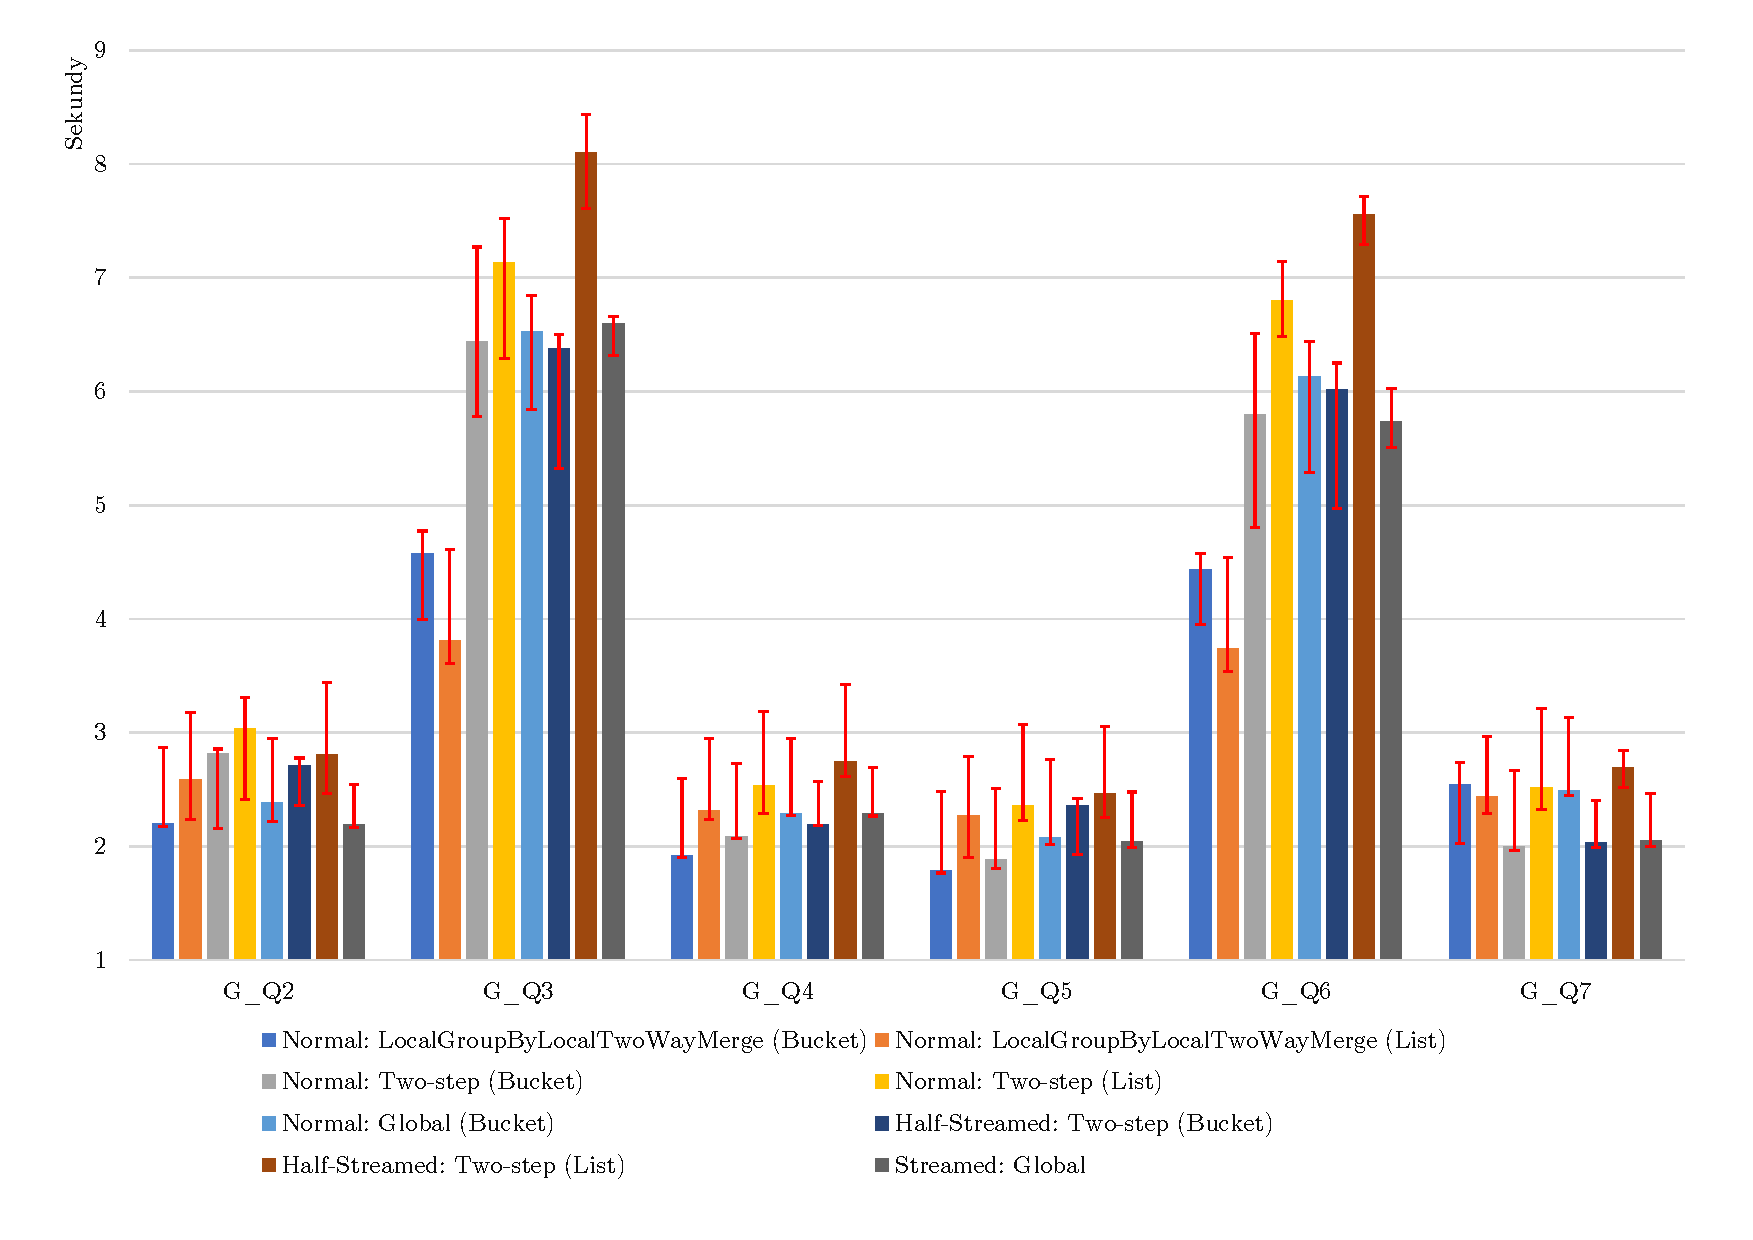
\includegraphics[width=\linewidth]{../img/amazonGroupByPar.pdf}\centering
\caption{Doba vykonání dotazů \textit{Group by} pro graf Amazon0601 (sekce \ref{tab.grafBase}). Běh osmi vláken.}
\label{figure.amazonGroupByPar}
\end{figure}
\begin{figure}[!htp]
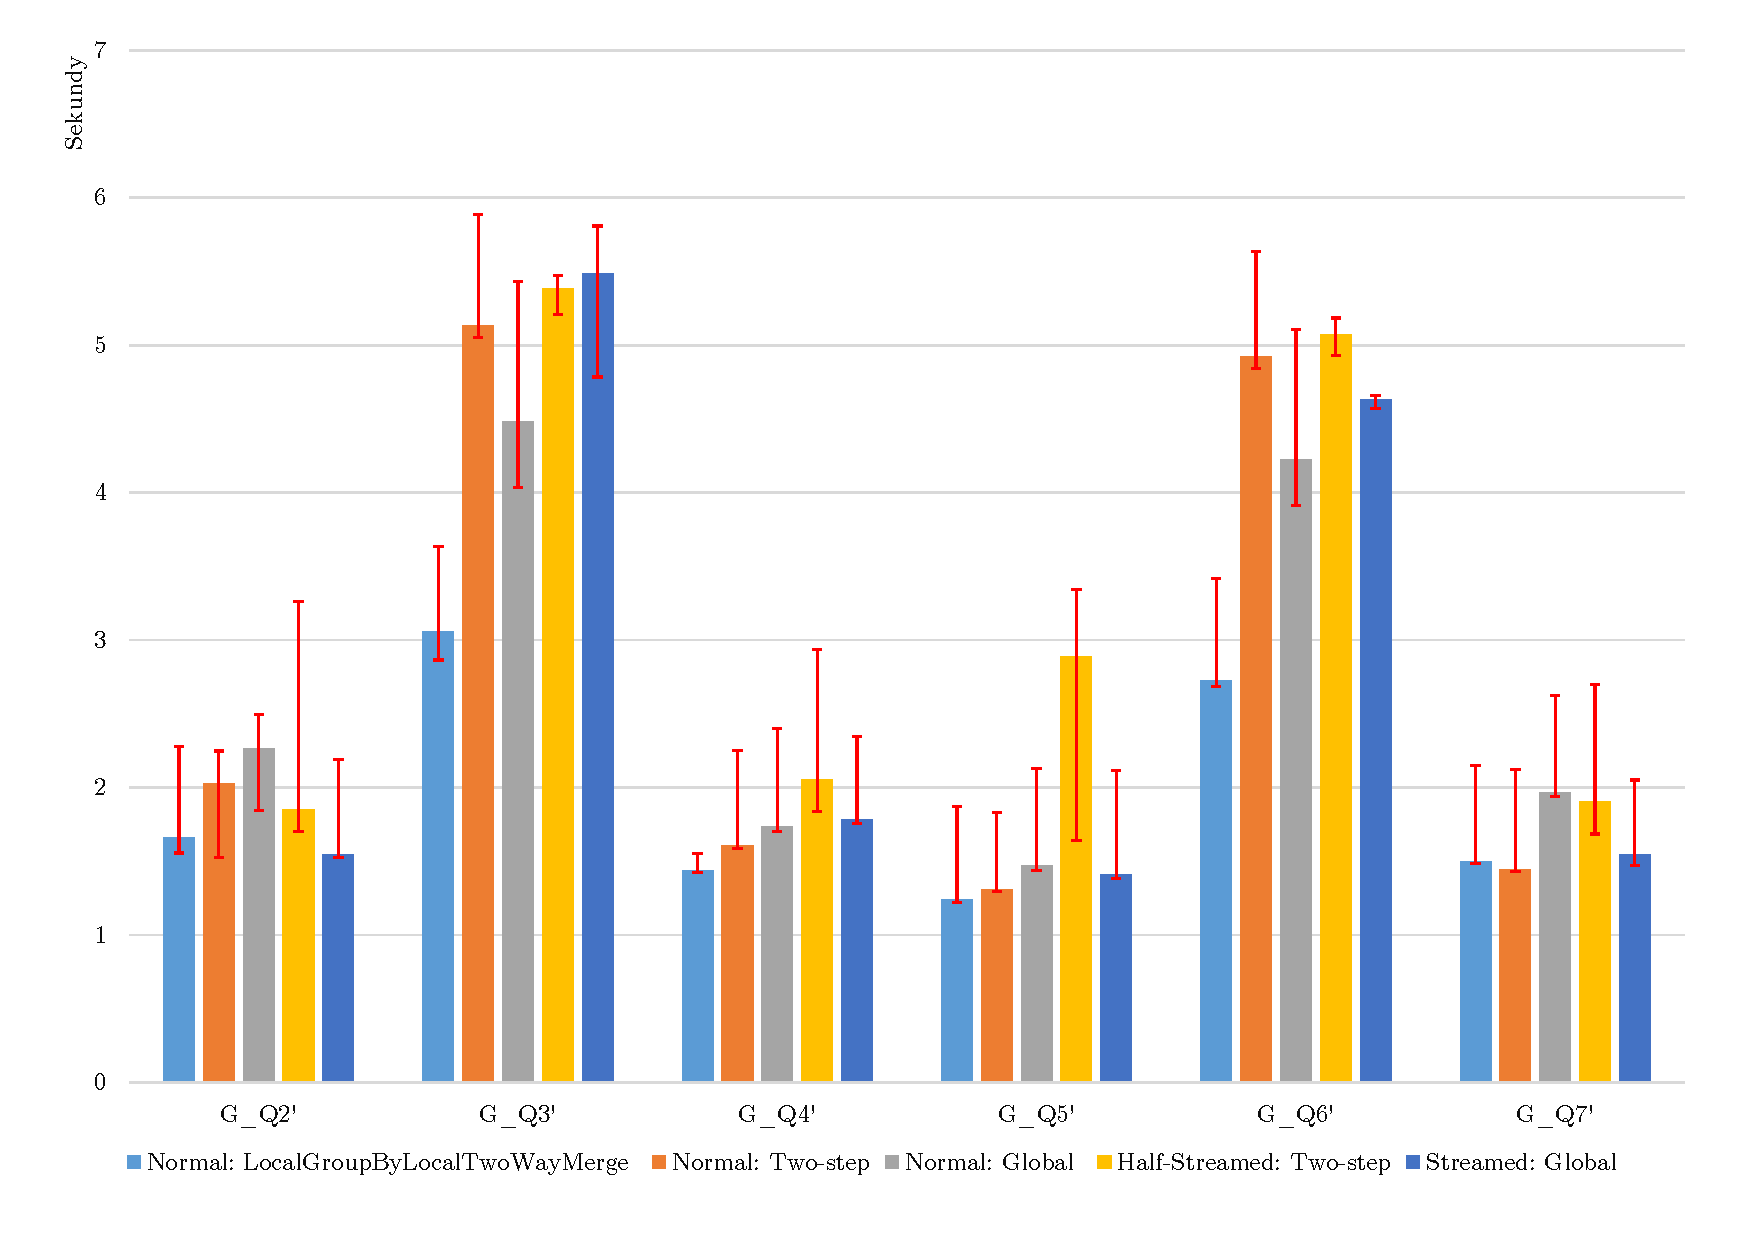
\includegraphics[width=\linewidth]{../img/amazonGroupByParNoAgg.pdf}\centering
\caption{Doba vykonání dotazů \textit{Group by} pro graf Amazon0601 (sekce \ref{tab.grafBase}) bez agregačních funkcí. Běh osmi vláken.}
\label{figure.amazonGroupByParNoAgg}
\end{figure}

\begin{figure}[!htp]
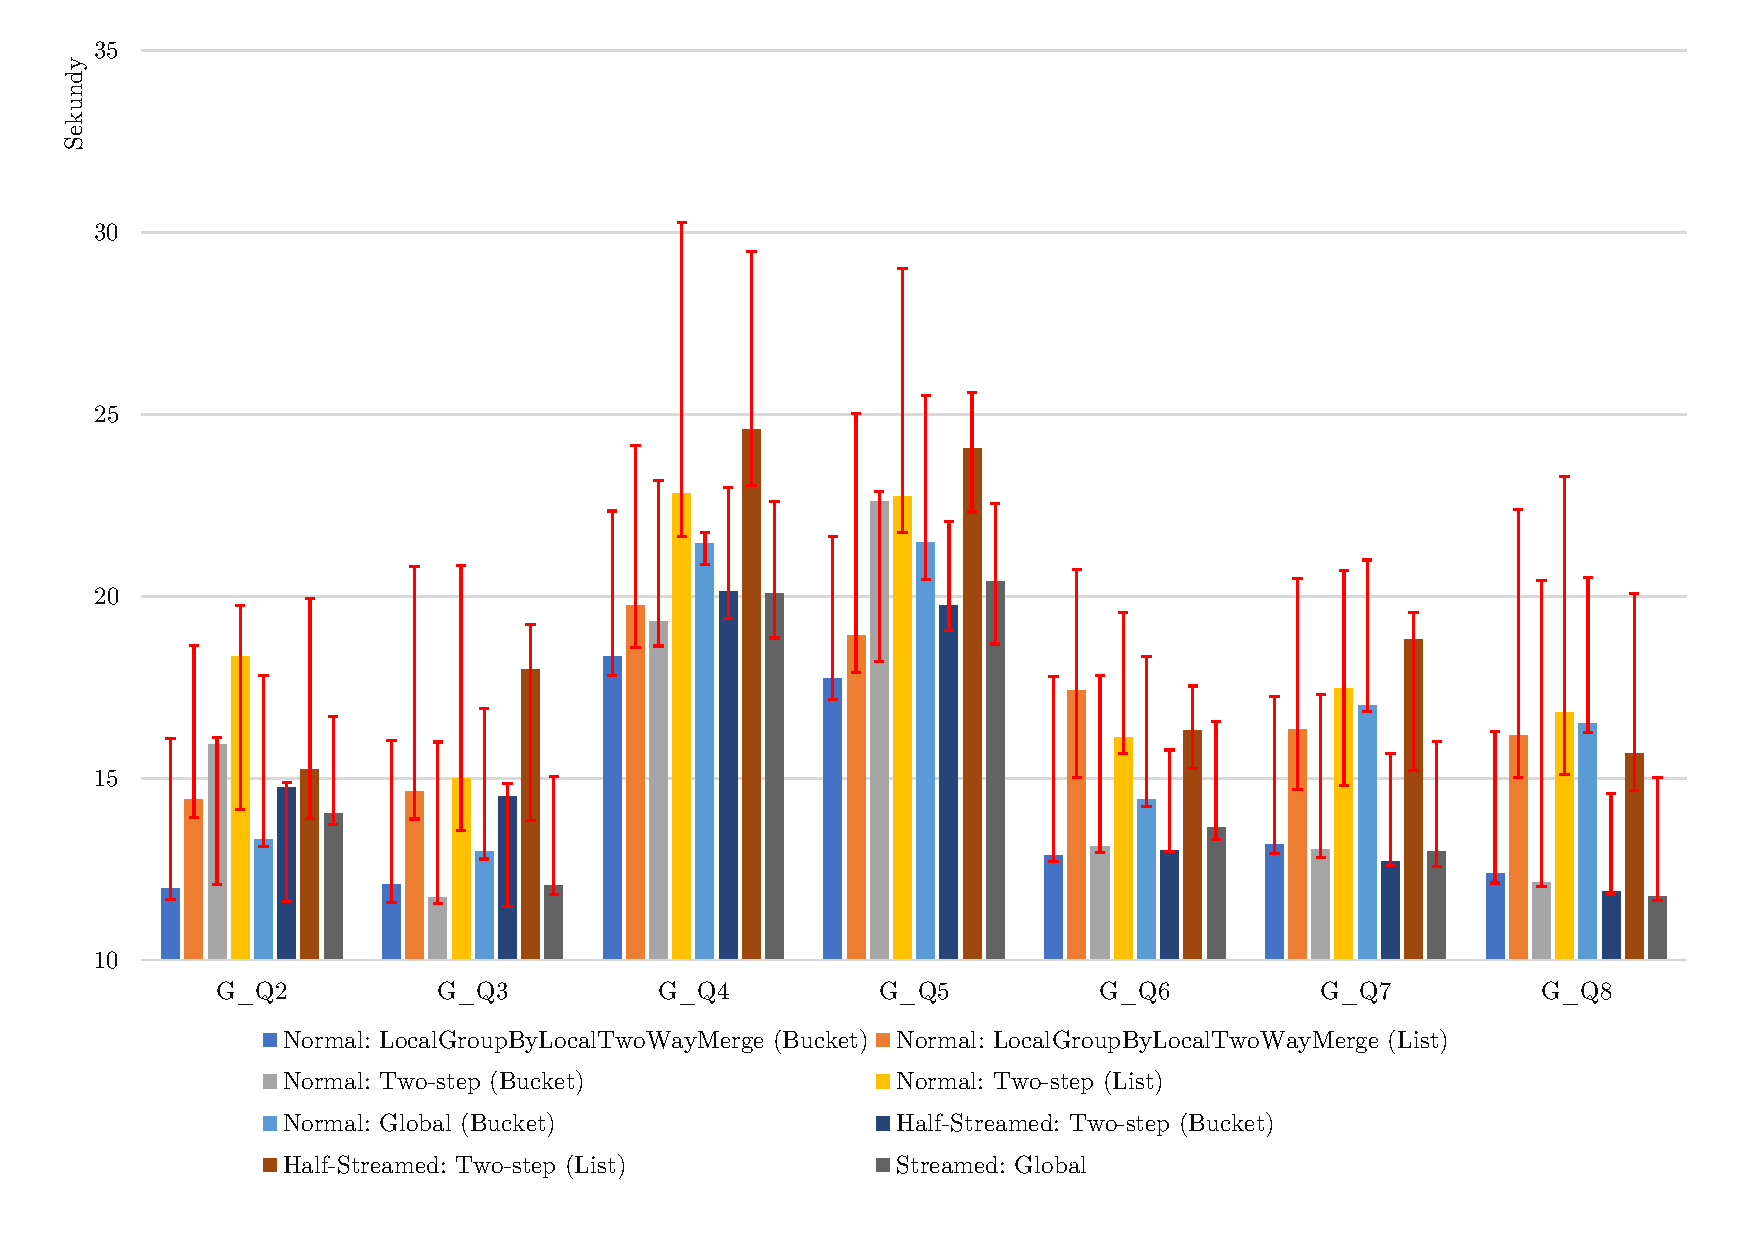
\includegraphics[width=\linewidth]{../img/webberkstanGroupByPar.pdf}\centering
\caption{Doba vykonání dotazů \textit{Group by} pro graf WebBerkStan (sekce \ref{tab.grafBase}). Běh osmi vláken.}
\label{figure.webberkstanGroupByPar}
\end{figure}
\begin{figure}[!htp]
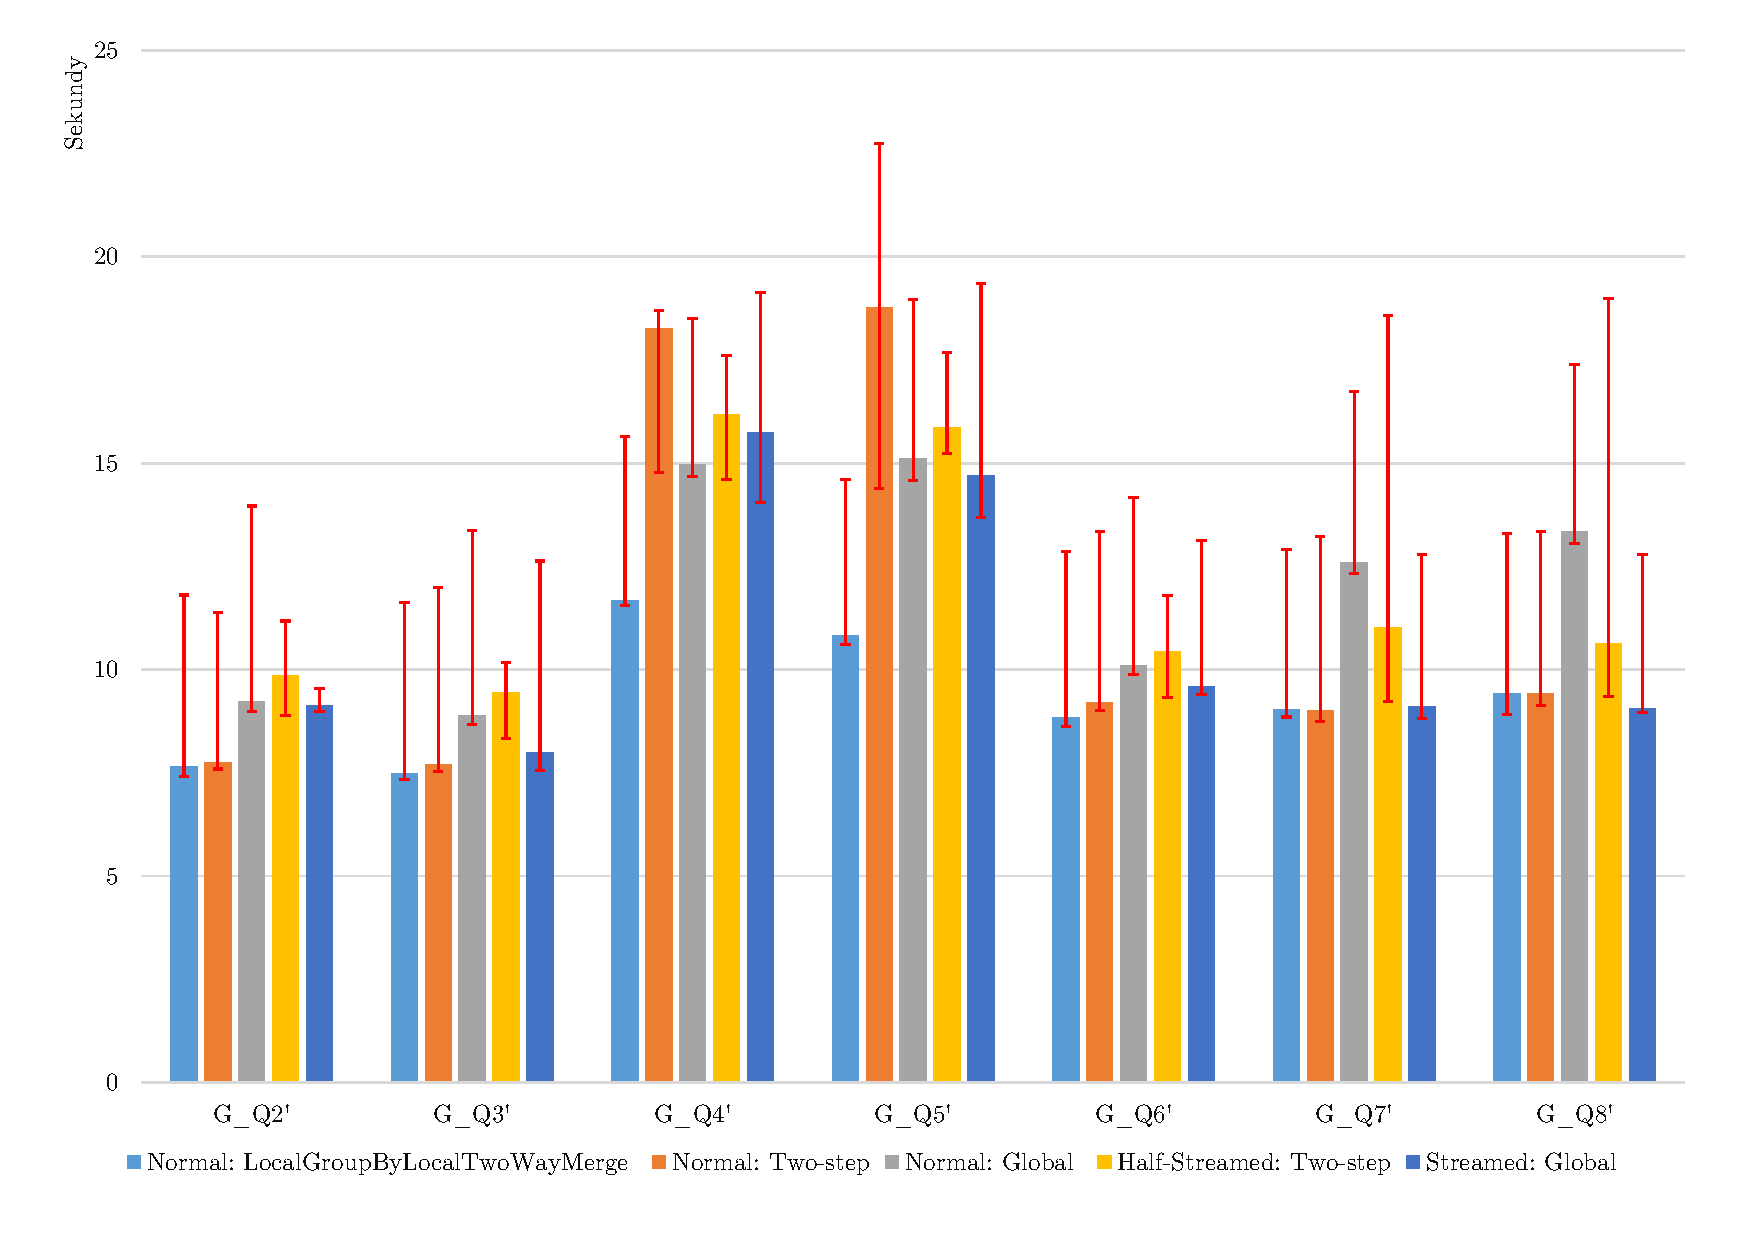
\includegraphics[width=\linewidth]{../img/webberkstanGroupByParNoAgg.pdf}\centering
\caption{Doba vykonání dotazů \textit{Group by} pro graf WebBerkStan (sekce \ref{tab.grafBase}) bez agregačních funkcí. Běh osmi vláken.}
\label{figure.webberkstanGroupByParNoAgg}
\end{figure}

\begin{figure}[!htp]
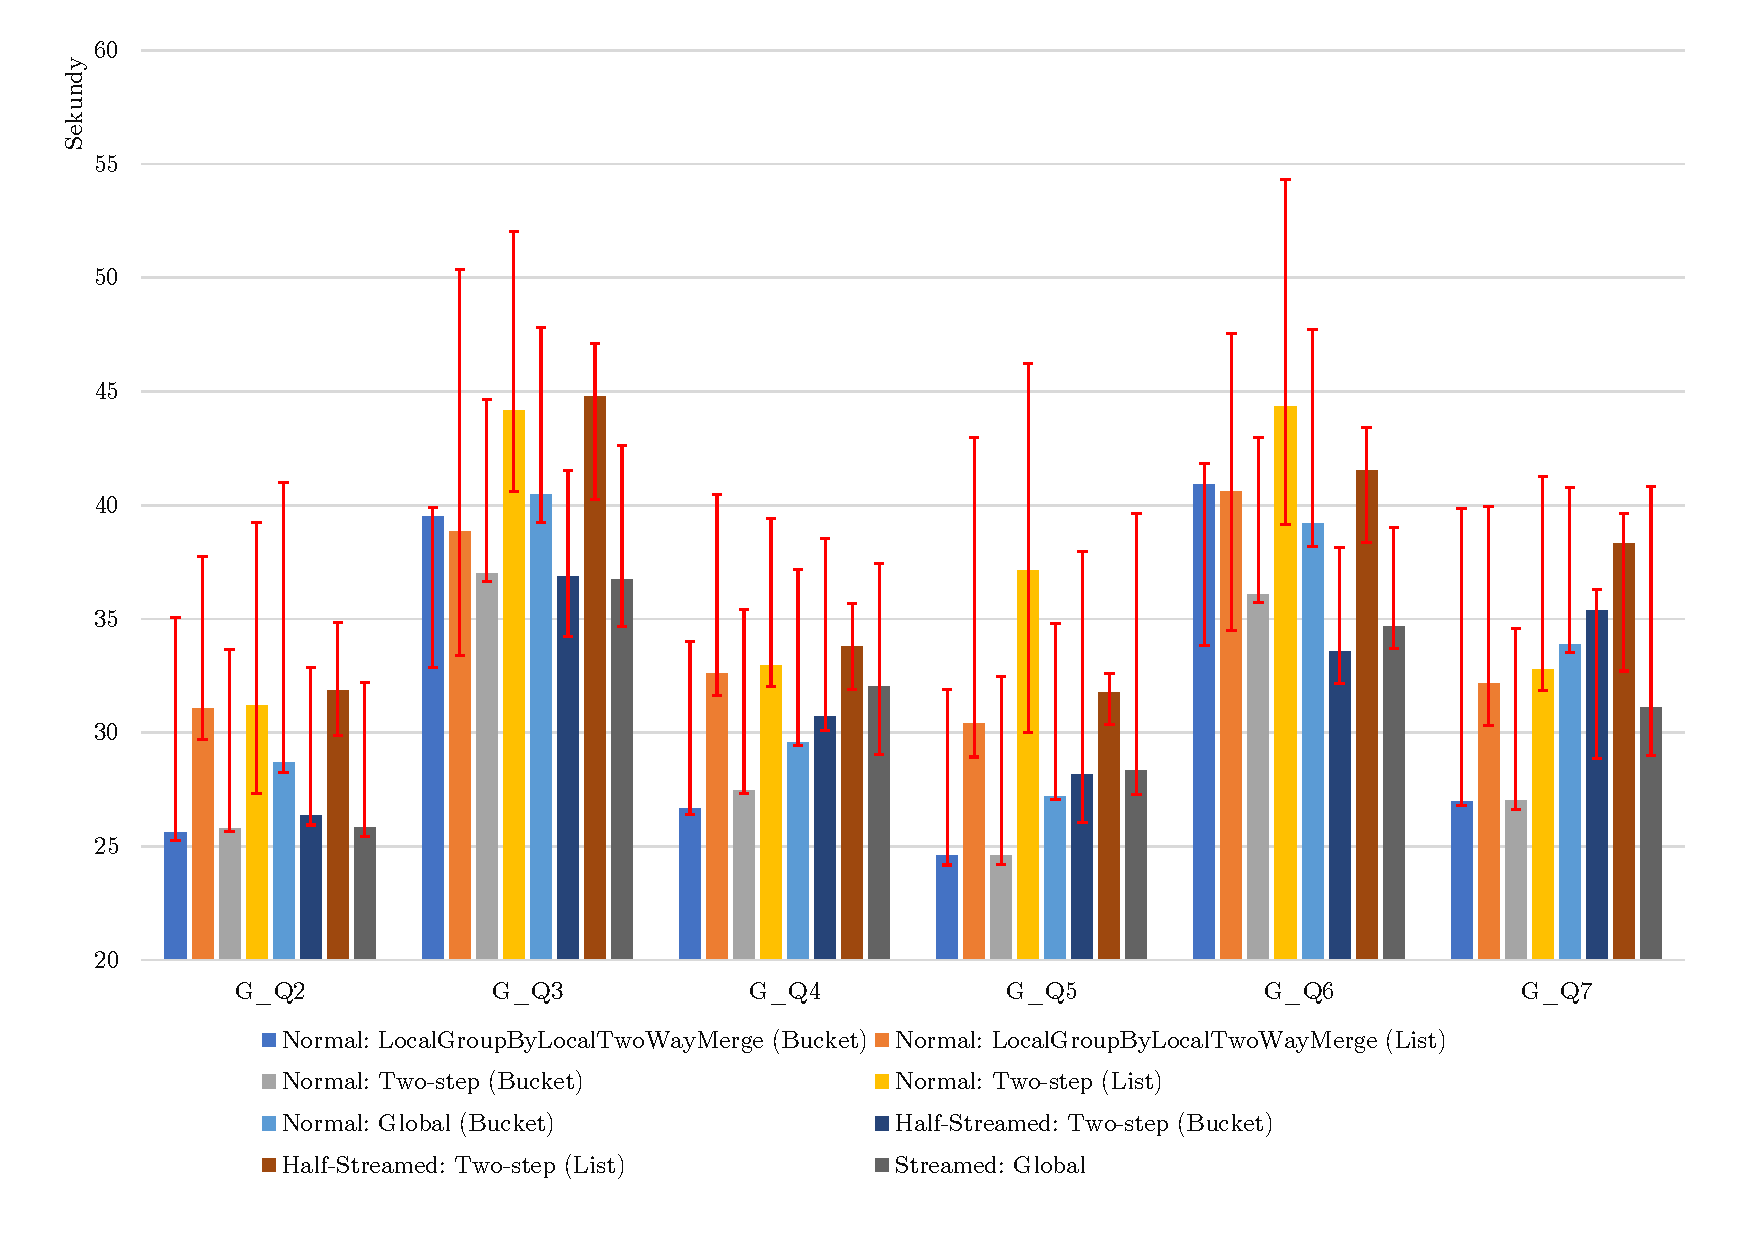
\includegraphics[width=\linewidth]{../img/skitterGroupByPar.pdf}\centering
\caption{Doba vykonání dotazů \textit{Group by} pro graf As-Skitter (sekce \ref{tab.grafBase}). Běh osmi vláken.}
\label{figure.skitterGroupByPar}
\end{figure}
\begin{figure}[!htp]
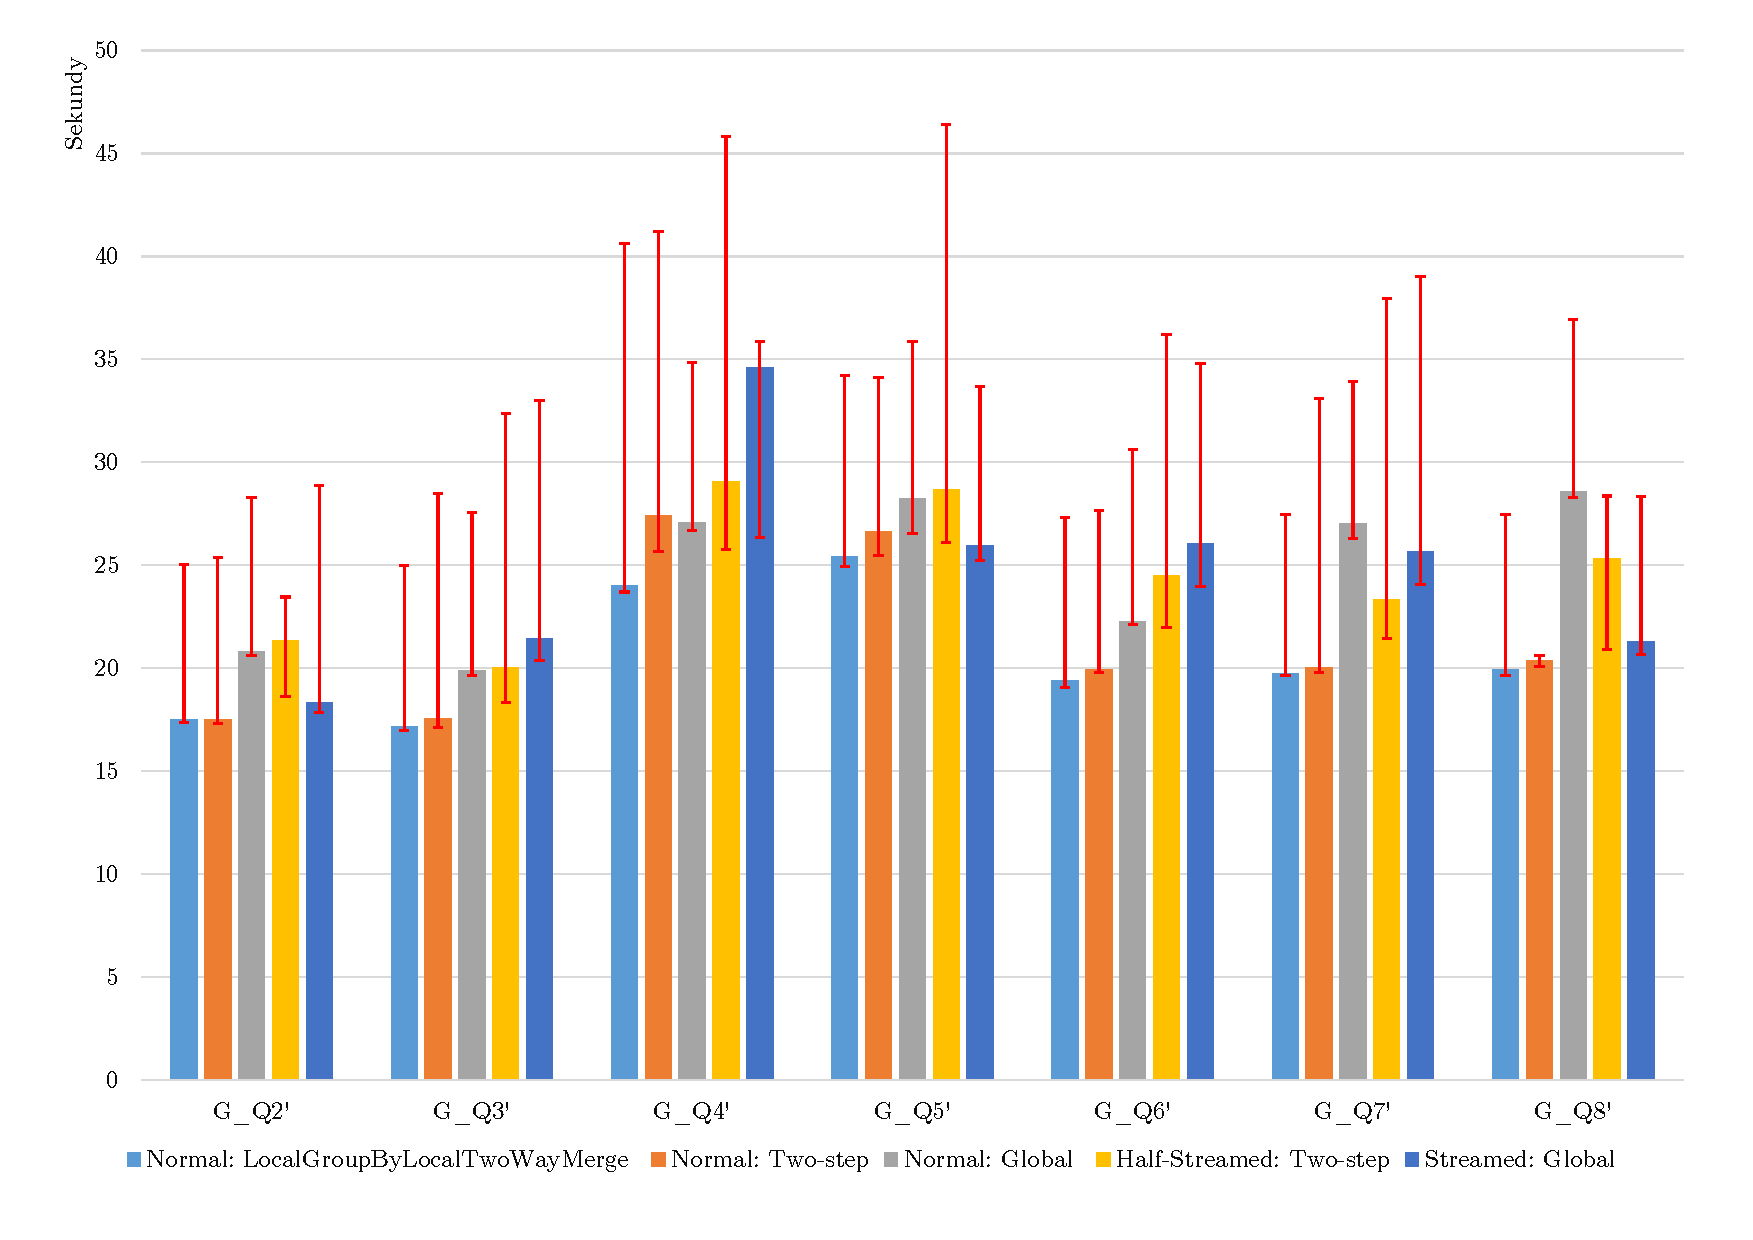
\includegraphics[width=\linewidth]{../img/skitterGroupByParNoAgg.pdf}\centering
\caption{Doba vykonání dotazů \textit{Group by} pro graf As-Skitter (sekce \ref{tab.grafBase}) bez agregačních funkcí. Běh osmi vláken.}
\label{figure.skitterGroupByParNoAgg}
\end{figure}
\bigskip

\subsubsection{Obecné shrnutí Single group Group by řešení} \label{expr.results.groupby.sinleGroup}

Analýzu výsledků dotazu G\_Q1 uvádíme samostatně, protože testuje pouze agregační funkce a nikoliv seskupování.
Daný mód \textit{Group by} předpokládá, že všechny výsledky patří do stejné skupiny a tedy nedochází k seskupování ale pouze k výpočtu agregačních funkcí.
Jednovláknové \textbf{Normal} řešeni iteruje skrze všechny výsledky po dokončení vyhledávání a vypočte agregační funkce.
Jednovláknové \textbf{Half-Streamed} a \textbf{Streamed} řešení jsou totožná.
V průběhu prohledávání aktualizují hodnotu agregační funkce a výsledek zahodí. 
Paralelní \textbf{Normal} řešení všem vláknům přidělí stejný počet výsledků prohledávání a každé lokálně spočte hodnoty agregačních funkcí.
Po ukončení práce všech vláken jedno vybrané vlákno sloučí výsledky všech ostatních vláken. 
Řešení \textbf{Half-Streamed} provádí stejnou práci jako v jednovláknovém zpracování.
Po dokončení prohledávání dojde ke sloučení všech lokálních výsledků.
\textbf{Streamed} řešení pracuje se sdíleným úložištěm výsledků a používá thread-safe funkce k aktualizaci výsledků.
Obě řešení výsledky neukládají.

\begin{figure}[!htp]
    \centering
    \begin{minipage}{0.45\textwidth}
        \centering
        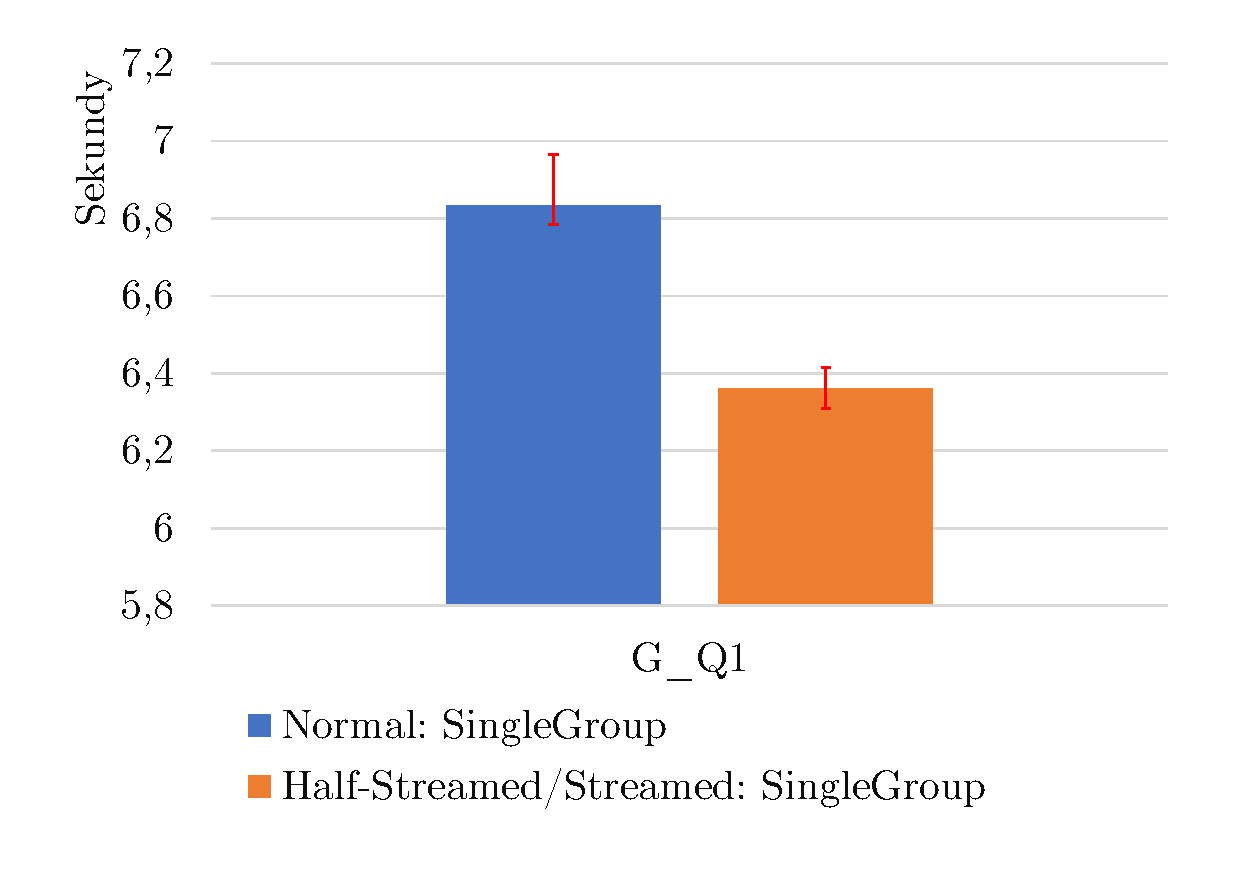
\includegraphics[width=0.9\textwidth]{../img/amazonGroupByQ1ST.pdf} % first figure itself
        \caption{Doba vykonání dotazu G\_Q1 pro graf Amazon0601 (sekce \ref{tab.grafBase}). Běh v jednom vláknu.}
        \label{figure.amazonGQ1ST}
    \end{minipage}\hfill
    \begin{minipage}{0.45\textwidth}
        \centering
        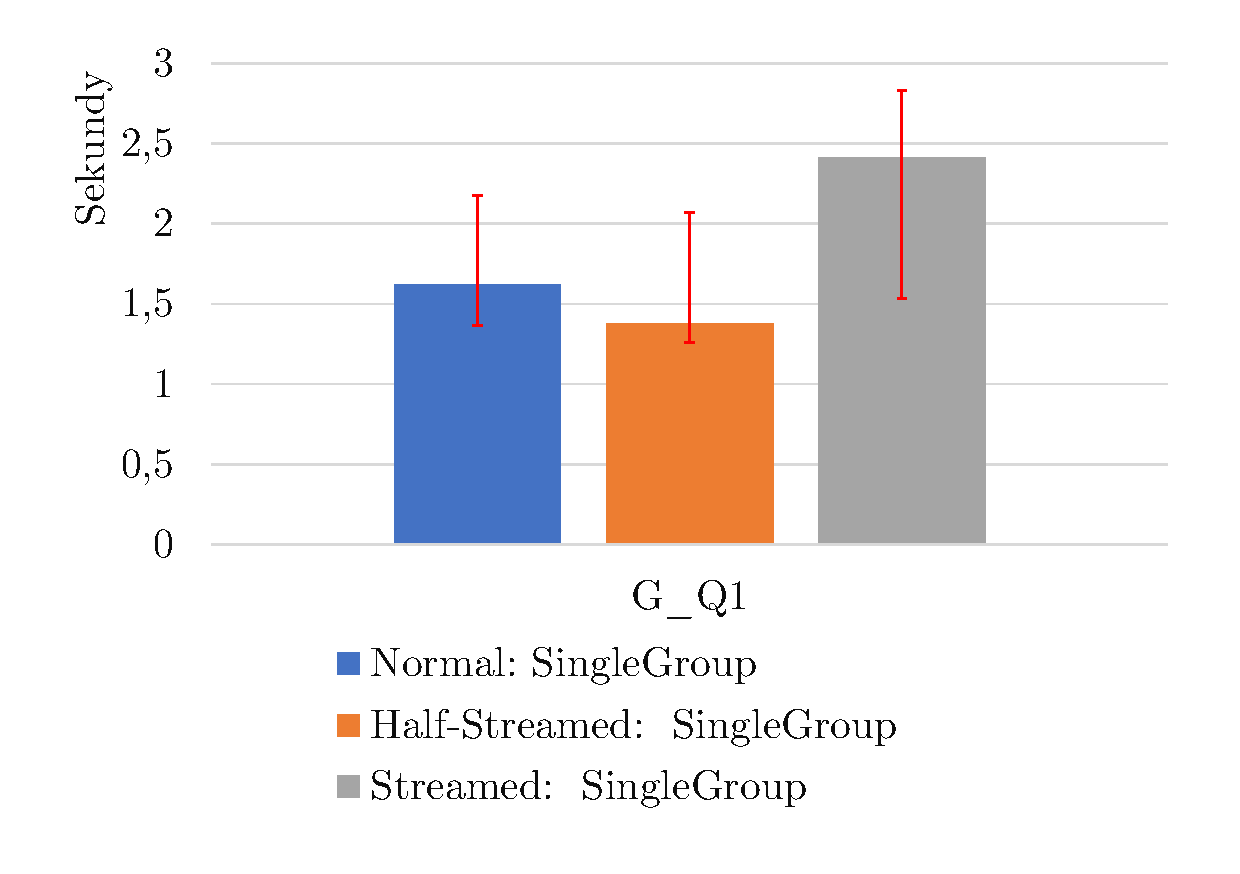
\includegraphics[width=0.9\textwidth]{../img/amazonGroupByQ1Par.pdf} % second figure itself
        \caption{Doba vykonání dotazu G\_Q1 pro graf Amazon0601 (sekce \ref{tab.grafBase}). Běh osmi vláken.}
        \label{figure.amazonGQ1Par}
    \end{minipage}
\end{figure}

\begin{figure}[!htp]
    \centering
    \begin{minipage}{0.45\textwidth}
        \centering
        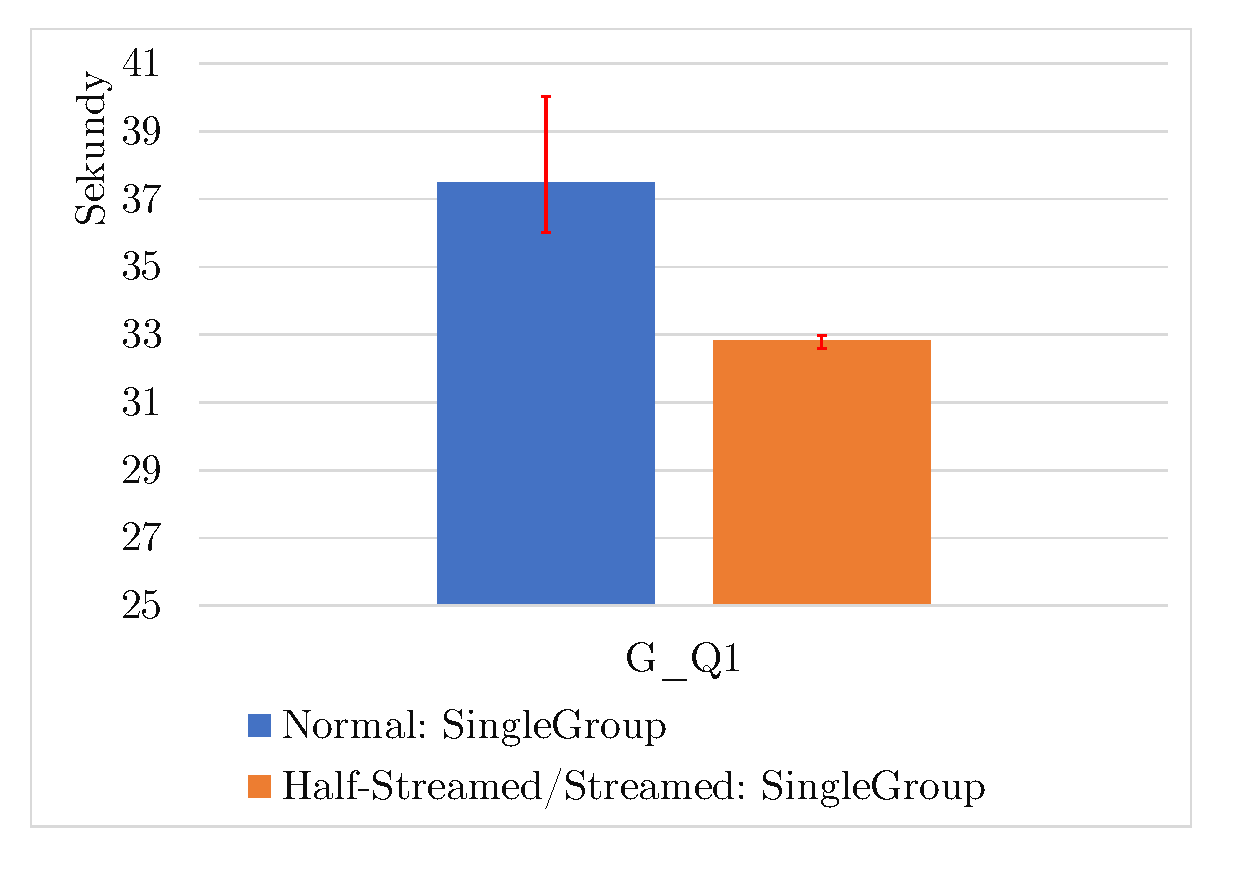
\includegraphics[width=0.9\textwidth]{../img/webberkstanGroupByQ1ST.pdf} % first figure itself
        \caption{Doba vykonání dotazu G\_Q1 pro graf WebBerkStan (sekce \ref{tab.grafBase}). Běh v jednom vláknu.}
        \label{figure.webberkstanGQ1ST}
    \end{minipage}\hfill
    \begin{minipage}{0.45\textwidth}
        \centering
        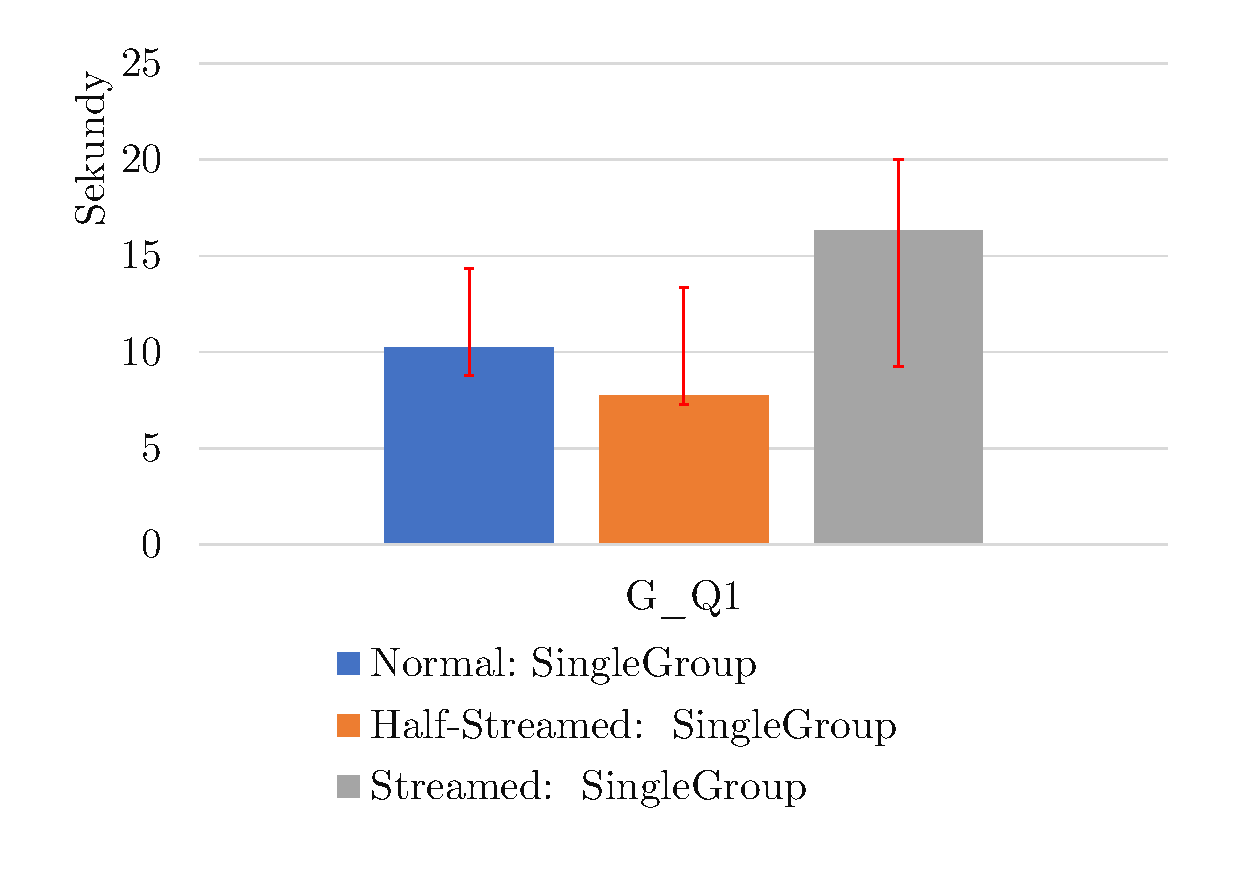
\includegraphics[width=0.9\textwidth]{../img/webberkstanGroupByQ1Par.pdf} % second figure itself
        \caption{Doba vykonání dotazu G\_Q1 pro graf WebBerkStan (sekce \ref{tab.grafBase}). Běh osmi vláken.}
        \label{figure.webberkstanGQ1Par}
    \end{minipage}
\end{figure}
\clearpage
\begin{figure}[!htp]
    \centering
    \begin{minipage}{0.45\textwidth}
        \centering
        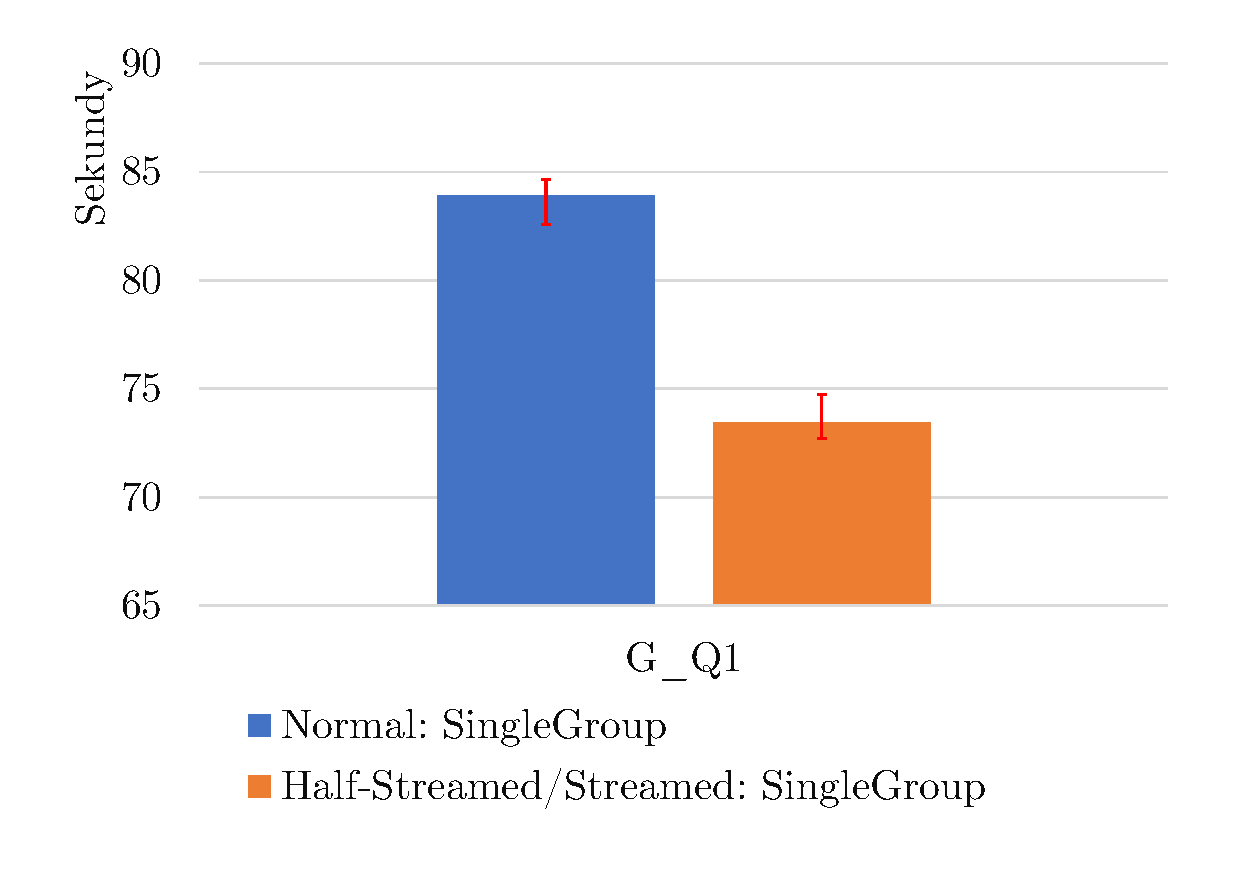
\includegraphics[width=0.9\textwidth]{../img/skitterGroupByQ1ST.pdf} % first figure itself
        \caption{Doba vykonání dotazu G\_Q1 pro graf As-Skitter (sekce \ref{tab.grafBase}). Běh v jednom vláknu.}
        \label{figure.skitterGQ1ST}
    \end{minipage}\hfill
    \begin{minipage}{0.45\textwidth}
        \centering
        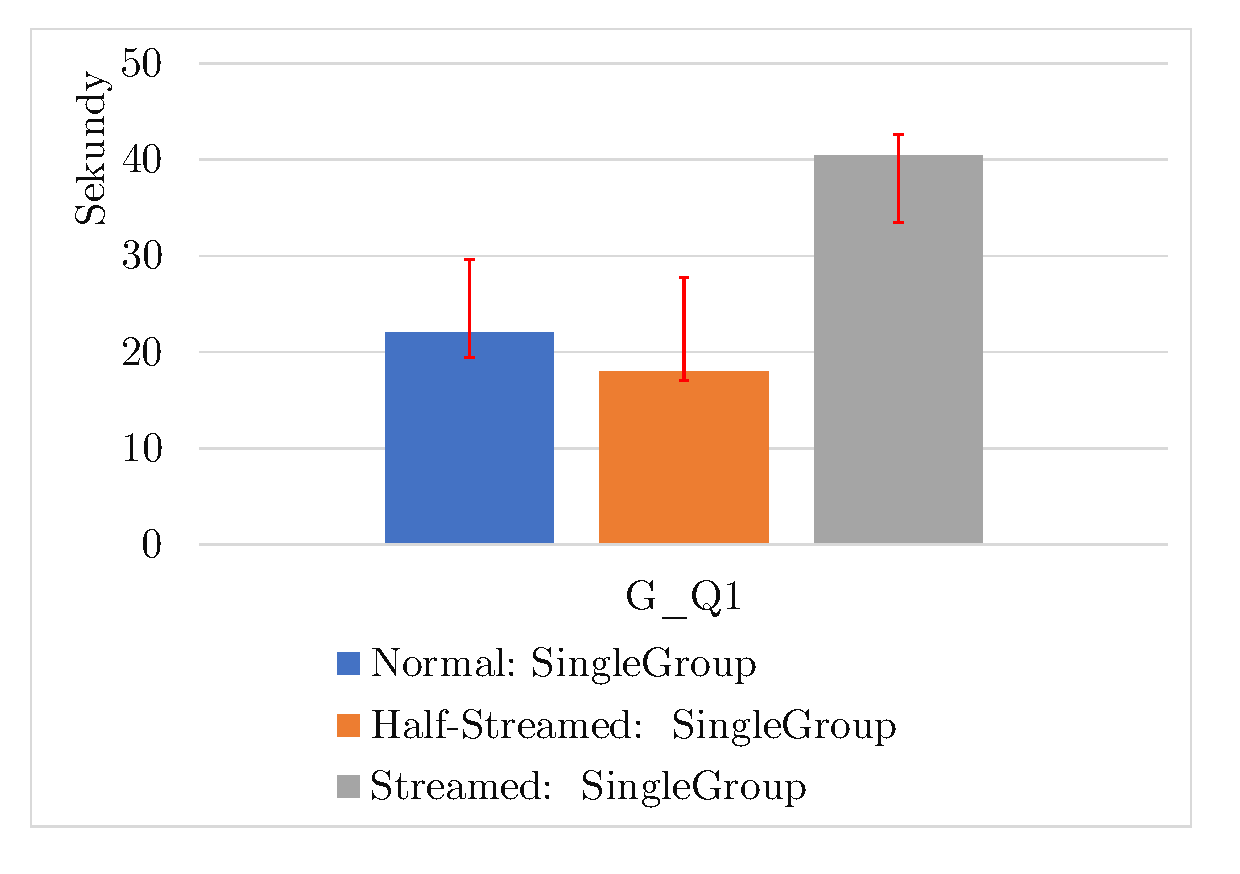
\includegraphics[width=0.9\textwidth]{../img/skitterGroupByQ1Par.pdf} % second figure itself
        \caption{Doba vykonání dotazu G\_Q1 pro graf As-Skitter (sekce \ref{tab.grafBase}). Běh osmi vláken.}
        \label{figure.skitterGQ1Par}
    \end{minipage}
\end{figure}

\subsubsection{Výsledky Single group Group by zpracování}

Na grafech \ref{figure.amazonGQ1ST} až \ref{figure.skitterGQ1Par} lze vidět značnou konzistenci mezi výsledky testování při nárůstu počtu výsledků vyhledávání.
\textbf{Half-Streamed} a \textbf{Streamed} řešení zde neukládá výsledky vyhledávání do tabulky, ale pouze na aktuální výsledek aplikuje agregační funkce a následně jej zahodí.
To způsobuje značnou výhodu oproti \textbf{Normal} řešení, které drží všechny výsledky v paměti.
Použijeme-li poznatky z sekce \ref{matchResults} o zpomalení způsobeném ukládáním výsledků do tabulky zjistíme (v našem případě jedné proměnné), že rozdíl mezi \textbf{Normal} a \textbf{Half-Streamed} řešením se pohybuje právě v rozsahu onoho zpomalení.
To platí pro běh jednoho vlákna i běhu osmi vláken. 
Problém představuje paralelní \textbf{Streamed} řešení, jelikož k jednomu výsledku přistupuje osm vláken najednou, což způsobuje značné zpomalení kvůli nutné synchronizaci při výpočtu funkcí \verb+min+ a \verb+avg+. 
Zrychlení je zde pouze v rozsahu $[1,81; 2,64]$-krát, zatímco u zbylých řešení je $[3,67; 4,61]$-krát.

Tímto jsme zakončili prezentaci výsledků. 
Všechna nasbíraná data použitá k tvorbě grafů je možné nalézt v příloze výsledků benchmarku (\ref{prilohy.grafyVysledky}). 



\chapter{Závěr}
%\addcontentsline{toc}{chapter}{Závěr}

Tady ma byt text

\section{Budoucí výzkum}


\begin{enumerate}


\item Rozšíření enginu o možnost zadat Order by a Group by společně.
Agregování v průběhu hledání se dá rozdělit na dvě hlavní části.
V první části lze navrhnout řešení pro dotazy, které obsahují třídění pouze podle klíčů skupin.
V druhé části je nutné vyřešit problém třídění pomocí výsledků agregačních funkcí.
Zde je největší problém fakt, že výsledky agregačních funkcí jsou známy pouze po dokončení Group by.

\item Testování daných řešení na grafech s reálnými Properties.
V našem testování jsme sice volili reálne grafy, ale jejich Properties jsme uměle vygenerovali.

\item Sledování obecného problému rozdělení dat při paralelizaci vylepšených řešení. 
Normal přistup má vždy všechna data připravená v paměti a při zpracování je rovnoměrně rozděluje mezi vlákny.
Vlákna tedy mají vždy stejný počet výsledků pro zpracování.
Navíc díky kompletnosti dat lze data optimálněji zpracovávat a použít větší množství obecných algoritmů.
Například při třídění jsme použili základní algoritmu Merge sort, který není možný aplikovat při třídění v průběhu vyhledávání.  
Rozdělení práce vylepšených řešení závísí na počtu vyhledaných výsledků v každém vlákně.
Mohou nastávát případy, kdy jedno vlákno má více výsledků ke zpracování než ostatní. 
Daný problém jsme se v našem řešení prohledávání snažili vyřešit pomocí přidělování malých skupin vrcholů vláknum.
Vlákno po prohledání daných vrcholů zažádalo o další.
Nicméně, dané řešení nemůže zaručit stoprocentně rovnoměrné rozdělení práce.
Bylo by vhodné prozkoumat, jak daná situace ovlivňuje naše řešení.

\item U Order by řešení jsme viděli značné zrychlení při třídění pomocí Properties v paralelizovaných řešeních.
Bylo by vhodné prozkoumat možnosti vytvoření globálních statistik pro každou Property a podrobněji zjistit možnosti rozdělení rozsahů přihrádek.
Samotné rozdělení přihrádek jsme pro řetězce zpracovali pouze s předpokladem, že se jedná o ASCII znaky.
V budoucí práci je možné zkoumat rozdělování i pro složitější znakové sady.

\item V paralelních Group by řešeních by bylo vhodné prozkoumat podrobněji skalabilitu daných řešení pro rozličné počty vláken.
Pokud možno, také možnosti jiných paralelních map.
 
\end{enumerate}

%%% Seznam použité literatury
\nocite{microsoft}
%%% Seznam použité literatury (bibliografie)
%%%
%%% Pro vytváření bibliografie používáme bibTeX. Ten zpracovává
%%% citace v textu (např. makro \cite{...}) a vyhledává k nim literaturu
%%% v souboru literatura.bib.
%%%
%%% Příkaz \bibliographystyle určuje, jakým stylem budou citovány odkazy
%%% v textu. V závorce je název zvoleného souboru .bst. Styly plainnat
%%% a unsrt jsou standardní součástí latexových distribucí. Styl czplainnat
%%% je dodáván s touto šablonou a bibTeX ho hledá v aktuálním adresáři.

\bibliographystyle{czplainnat}    %% Autor (rok) s českými spojkami
% \bibliographystyle{plainnat}    %% Autor (rok) s anglickými spojkami
% \bibliographystyle{unsrt}       %% [číslo]

\renewcommand{\bibname}{Seznam použité literatury}

%%% Vytvoření seznamu literatury. Pozor, pokud jste necitovali ani jednu
%%% položku, seznam se automaticky vynechá.

\bibliography{literatura}

%%% Kdybyste chtěli bibliografii vytvářet ručně (bez bibTeXu), lze to udělat
%%% následovně. V takovém případě se řiďte normou ISO 690 a zvyklostmi v oboru.

% \begin{thebibliography}{99}
%
% \bibitem{lamport94}
%   {\sc Lamport,} Leslie.
%   \emph{\LaTeX: A Document Preparation System}.
%   2. vydání.
%   Massachusetts: Addison Wesley, 1994.
%   ISBN 0-201-52983-1.
%
% \end{thebibliography}


%%% Obrázky v bakalářské práci
%%% (pokud jich je malé množství, obvykle není třeba seznam uvádět)
\listoffigures

%%% Tabulky v bakalářské práci (opět nemusí být nutné uvádět)
%%% U matematických prací může být lepší přemístit seznam tabulek na začátek práce.
\listoftables

%%% Použité zkratky v bakalářské práci (opět nemusí být nutné uvádět)
%%% U matematických prací může být lepší přemístit seznam zkratek na začátek práce.
%%%\chapwithtoc{Seznam použitých zkratek}

%%% Přílohy k bakalářské práci, existují-li. Každá příloha musí být alespoň jednou
%%% odkazována z vlastního textu práce. Přílohy se číslují.
%%%
%%% Do tištěné verze se spíše hodí přílohy, které lze číst a prohlížet (dodatečné
%%% tabulky a grafy, různé textové doplňky, ukázky výstupů z počítačových programů,
%%% apod.). Do elektronické verze se hodí přílohy, které budou spíše používány
%%% v elektronické podobě než čteny (zdrojové kódy programů, datové soubory,
%%% interaktivní grafy apod.). Elektronické přílohy se nahrávají do SISu a lze
%%% je také do práce vložit na CD/DVD. Povolené formáty souborů specifikuje
%%% opatření rektora č. 72/2017.
\appendix
\chapter{Přílohy}

\section{Benchmark stromy vůči polím}
\label{prilohy.benchtreevsarray}

Součástí této přílohy jsou zdrojové kódy benchmarku použitého k testování vybraných indexačních struktur.
Benchmark je použit v sekci \ref{anal.ordeby.single}.

\section{Online Git repozitář}
\label{prilohy.repo}

V době vydání tohoto textu probíhal vývoj dotazovacího enginu na GitHubu.

\begin{center}
\url{https://github.com/goramartin/QueryEngine}
\end{center}

\section{Zdrojové kódy}
\label{prilohy.kod}

Přílohou této bakalářské práce jsou zdrojové kódy dotazovacího enginu, benchmarku a použité knihovny HPCsharp (sekce \ref{impl.appsolution}).
Vše zmíněné je přiloženo v rámci jednoho projektu Visual Studia 2019, kromě souborů Gitu. 


\section{Kód pro transformaci grafů}
\label{prilohy.codetransform}

Součástí této přílohy jsou zdrojové kódy programů na generování vstupních grafů pro experiment (kapitola \ref{expr}). 
Jedná se o soubory \textit{GraphDataBuilder.cs} a \textit{PropertyGenerator.cs}.

\section{Použité grafy při experimentu}
\label{prilohy.grafy}

Grafy použité při experimentu (kapitola \ref{expr}) jsou vloženy do odpovídajících složek dle jejich názvů. 

\section{Výsledky benchmarku pro jednotlivé grafy}
\label{prilohy.grafyVysledky}

Součástí této přílohy je výstup benchmarku při vykonaném experimentu (kapitola \ref{expr}).
Soubory jsou rozděleny do složek podle názvů grafů.
Samotné výstupy nejsou nijak setříděny.



%%\section{druha priloha}

Priloha po prvni strance priloh


\openright
\end{document}
